%%%%%%%%%%%%%%%%%%%%%%%%%%%%%%%%%%%%%%%%%
% kaobook
% LaTeX Class
% Version 0.9.8 (2021/08/23)
%
% For the latest template development version and to make contributions:
% https://github.com/fmarotta/kaobook
%
% Authors:
% Federico Marotta (federicomarotta@mail.com)
% Based on the doctoral thesis of Ken Arroyo Ohori (https://3d.bk.tudelft.nl/ken/en)
% and on the Tufte-LaTeX class.
%
% License:
% LPPL (see included MANIFEST.md file)
%%%%%%%%%%%%%%%%%%%%%%%%%%%%%%%%%%%%%%%%%

\documentclass[
    a4paper, % page size
    fontsize=10pt, % font size
    twoside=true, % layouts for even and odd pages (in particular, if twoside=true, the margin column will be always on the outside)
	numbers=noenddot, % dots after chapter numbers (option are: enddot, noenddot and auto)
	fontmethod=tex, % "modern" with XeLaTeX or LuaTex; "tex" is the default for PdfLaTex
]{kaobook}

% clean start

% Choose the language
\ifxetexorluatex
	\usepackage{polyglossia}
	\setmainlanguage{english}
\else
	\usepackage[ngerman, english]{babel} % Load characters and hyphenation
\fi
\usepackage[english=american]{csquotes}	% English quotes

\usepackage{enumitem}

\usepackage{longtable}
\usepackage{booktabs}
\usepackage{tabularx}
\usepackage{siunitx}
\sisetup{
   separate-uncertainty
}
\usepackage{physics}


% Load the bibliography package
\usepackage[giveninits=true]{kaobiblio}
\addbibresource{references.bib} % Bibliography file

\ifdefined\rm
\renewcommand{\rm}{\mathrm}
\else
\newcommand{\rm}{\mathrm}
\fi

\ifdefined\gev
\renewcommand{\gev}{\giga\electronvolt}
\else
\newcommand{\gev}{\giga\electronvolt}
\fi

\ifdefined\mev
\renewcommand{\mev}{\mega\electronvolt}
\else
\newcommand{\mev}{\mega\electronvolt}
\fi

% define HNL mixing abbreviations
\def\ue4{$|U_{e4}|^2$}
\def\um4{$|U_{\mu4}|^2$}
\def\ut4{$|U_{\tau4}|^2$}


% Load mathematical packages for theorems and related environments
\usepackage[framed=true]{kaotheorems}
\usepackage{amsmath}

% Load the package for hyperreferences
\usepackage{kaorefs}

\usepackage{caption}
\usepackage{subcaption}

\graphicspath{{./}{figures/}} % Paths in which to look for images

% \makeindex[columns=3, title=Alphabetical Index, intoc] % Make LaTeX produce the files required to compile the index


% for Alex' crazy tikz stuff...
\usepackage{pgfplots}
\usepackage{pgfplotstable}
\usepgfplotslibrary{fillbetween}

\ifxetexorluatex
    % do nothing
\else
    \DeclareUnicodeCharacter{2212}{−}
\fi

\usepgfplotslibrary{groupplots,dateplot}
\usetikzlibrary{patterns,shapes,arrows}
\usetikzlibrary{fadings}
\pgfplotsset{compat=newest}

\usepackage{feynmp-auto}
\usepackage[compat=1.1.0]{tikz-feynman}

% global color definitions
\definecolor{black}{RGB}{0,0,0}
\definecolor{orange}{RGB}{230, 159, 0}
\definecolor{skyblue}{RGB}{86, 180, 233}
\definecolor{bluishgreen}{RGB}{0, 158, 115}
\definecolor{yellow}{RGB}{240, 228, 66}
\definecolor{blue}{RGB}{0, 114, 178}
\definecolor{vermilion}{RGB}{213, 94, 0}
\definecolor{reddishpurple}{RGB}{204, 121, 167}

\definecolor{tab_orange}{RGB}{255, 128, 14}
\definecolor{tab_blue}{RGB}{0, 107, 164}

\definecolor{lightgray204}{RGB}{204,204,204}

\tikzstyle{nue_color}=[orange]
\tikzstyle{numu_color}=[bluishgreen]
\tikzstyle{nutau_color}=[skyblue]
% color for any "all NC" plots
\tikzstyle{nc_color}=[reddishpurple]
\tikzstyle{noise_color}=[blue]
\tikzstyle{muon_color}=[vermilion]
% color for all combined nu flavors
\tikzstyle{nu_color}=[bluishgreen]

% plot an error band assuming that a table has been loaded.
% Syntax: \ploterrorband[style]{column_name}{scale_factor}
% The column name and the column "column_name__err" must exist. The
% scale factor scales the entire error band at once.
\newcommand{\ploterrorband}[3][black]{
	\addplot[const plot, #1, thick] table [x=bin_edges, y expr=\thisrow{#2} * #3] from \table;
    \addplot[const plot, #1, thin, name path=err_lo, forget plot] table[x=bin_edges, y expr=(\thisrow{#2}-\thisrow{#2__err}) * #3] from \table;
    \addplot[const plot, #1, thin, name path=err_hi, forget plot] table[x=bin_edges, y expr=(\thisrow{#2}+\thisrow{#2__err}) * #3] from \table;
    \addplot[#1, opacity=0.5, forget plot] fill between[of = err_lo and err_hi];
}

\newcommand{\plotratioerrorband}[3][black]{
	\addplot[const plot, #1, thick] table [x=bin_edges, y expr=\thisrow{#2} / \thisrow{#3}] from \table;

    \addplot[const plot, #1, thin, name path=err_lo, forget plot] table[x=bin_edges,
    y expr=
    	\thisrow{#2} / \thisrow{#3}
		-
		sqrt(
            (\thisrow{#2} * \thisrow{#3__err})^2 + (\thisrow{#3} * \thisrow{#2__err})^2 - (2 * \thisrow{#2} * \thisrow{#3} * \thisrow{#2__err}^2)
		) / \thisrow{#3}^2
	] from \table;

	\addplot[const plot, #1, thin, name path=err_hi, forget plot] table[x=bin_edges,
    y expr=
    	\thisrow{#2} / \thisrow{#3}
		+
		sqrt(
            (\thisrow{#2} * \thisrow{#3__err})^2 + (\thisrow{#3} * \thisrow{#2__err})^2 - (2 * \thisrow{#2} * \thisrow{#3} * \thisrow{#2__err}^2)
		) / \thisrow{#3}^2
	] from \table;

    \addplot[#1, opacity=0.5, forget plot] fill between[of = err_lo and err_hi];
}


\pgfplotsset{error bar legend/.style={%
    /pgfplots/legend image code/.prefix code={%
      \pgfkeysgetvalue{/pgfplots/error bars/error mark}{\pgfplotserrorbarsmark}%
      \draw[%
        /pgfplots/every error bar,
        mark=\pgfplotserrorbarsmark,
        /pgfplots/error bars/error mark options,
        sharp plot,
        ##1
      ] plot coordinates {(0.3cm, -0.1cm) (0.3cm, 0.1cm)};%
    }
  }
}

\newcommand{\ploterrorbar}[2][black]{
    \addplot[
        mark=*,
        mark options={scale=0.5, fill=black},
        #1,
        only marks,
        error bar legend,
        error bars/.cd,
        x dir=none,
        y dir=both,
        y explicit
    ] table [x=bin_midpoints, y=#2, y error=#2__err]  from \table;
}

% This package changes the font to serif when compiling with Lualatex (and doesn't)
% work correctly without Lualatex.
%\usepackage{helvet}
\usepackage[eulergreek]{sansmath}
\pgfplotsset{
    tick label style = {font=\footnotesize\sansmath\sffamily},
    every axis label = {font=\footnotesize\sansmath\sffamily},
    % the eulergreek style for math looks oddly different from the
    % rest of the document, so we omit \sansmath here
    label style = {font=\footnotesize\sffamily},
    % global legend style applied to all plots (set per plot to override)
    legend style = {
        font=\footnotesize\sffamily,
        fill opacity=0.8,
        draw opacity=1,
        text opacity=1,
        at={(0.5,0.95)},
        anchor=north,
        draw=lightgray204,
        % hack to get better legend spacing, see
        % https://tex.stackexchange.com/questions/18152/how-can-i-adjust-the-horizontal-spacing-between-legend-entries-in-pgfplots
        /tikz/every even column/.append style={column sep=0.1cm}
    },
    legend cell align={left}
}

\tikzstyle{plot annotation}=[
    font=\footnotesize\sffamily,
    fill opacity=0.8,
    draw opacity=1,
    text opacity=1,
    draw=lightgray204,
    fill=white
]

\begin{document} 

\frontmatter

\thispagestyle{plain}
\begin{center}
	\vspace*{1cm}

	\LARGE
	\textbf{Measurement of  Astrophysical Neutrino flavour composition with Twelve Years of IceCube Data}
	\large

	\vspace{0.8cm}

	\textbf{Dissertation}\\
	zur Erlangung des akademischen Grades\\
	doctor rerum naturalium \\
	(Dr. rer. nat.) \\

	\vspace{0.5cm}

	im Fach: Physik \\
	Spezialisierung: Experimentalphysik\\

	\vspace{0.5cm}

	eingereicht an der \\
	Mathematisch-Naturwissenschaftlichen Fakultät\\
	der Humboldt-Universität zu Berlin\\

	\vspace{0.5cm}

	von\\
	\textbf{Neha Lad M. Sc.}\\
	%	\vspace{0.8cm}
	geboren am 18. April 1995\\
	

	\vspace{0.5cm}

	Präsidentin der Humboldt-Universität zu Berlin \\
	Prof. Dr. Julia von Blumenthal \\

	\vspace{0.5cm}

	Dekanin der Mathematisch-Naturwissenschaftlichen Fakultät \\
	Prof. Dr. Caren Tischendorf \\

	\vspace{0.5cm}

	% % uncomment for publication
	% Gutachter:innen:
	% Prof. Dr. Marek Kowalski, Humboldt-Universität zu Berlin \\
	% Prof. Dr. Joachim Kopp, Johannes Gutenberg-Universität Mainz \\
	% Dr. Priscilla Pani, DESY Zeuthen \\

	% \vspace{0.5cm}

	% Tag der mündlichen Prüfung: xx.xx.2024

\end{center}

\newpage
\thispagestyle{plain}

\begin{flushleft}	
	\vspace*{8cm}
	
	\textbf{Copyright Notice} \\
	This book is released into the public domain using the CC-BY-4.0 code.

	To view a copy of the CC-BY-4.0 code, visit: \\\url{https://creativecommons.org/licenses/by/4.0/}

	\medskip
	
	\textbf{Colophon} \\
	This document was typeset with the help of \href{https://sourceforge.net/projects/koma-script/}{\KOMAScript} and \href{https://www.latex-project.org/}{\LaTeX} using the open-source \href{https://github.com/fmarotta/kaobook/}{kaobook} template class. \\
	
	\medskip
	
	The source code of this thesis is available  at: \\\url{https://github.com/NehaLad9/thesis.git}

	\medskip

	\textbf{Publisher} \\
	First printed in Nov 2024 by Humboldt Universität zu Berlin
	% \todo[inline, noinlinepar]{add when first printed and by whom}
\end{flushleft}
	

% \newpage
% \thispagestyle{plain}

% \vspace*{5.0cm}

% \flushright \textit{Dada, this one is for you}\\
% \flushright \textit{Thank you for teaching me to always be curious, I miss you.}

\cleardoublepage


\cleardoublepage
\phantomsection

\chapter{Abstract}
Cosmic rays and high-energy neutrinos share a fundamental connection, as both are produced in extreme astrophysical environments where cosmic rays interact with matter or photons near their acceleration sites to produce neutrinos. The observable flavor composition of neutrinos on Earth offers critical insights into potential production mechanisms at these cosmic sources. Due to neutrino oscillations over cosmic baselines, tau neutrinos—which are not directly produced at the sources—are expected to appear by the time neutrinos reach Earth, making their detection essential for studies of astrophysical neutrino sources and flavor evolution. 

This thesis aims to measure the flavor composition of high-energy astrophysical neutrinos, with a particular focus on detecting tau neutrino events within a high-energy starting event sample collected by the IceCube Neutrino Observatory in Twelve years of its livetime. Using a ternary classifier, high energy starting events are reconstructed into three distinct morphologies—single cascade, double cascade, and track—primarily associated with the three neutrino flavors (\( \nu_e \), \( \nu_\tau \), and \( \nu_\mu \)). Five events were identified as double cascades, including four previously unobserved, along with 64 single cascades and 28 starting tracks, consistent with expectations from a single power-law spectrum of neutrino. Significant improvements were implemented in both simulations and reconstruction methods compared to prior analyses, including corrections for cross-sections, tau lepton polarization, and updated neutrino weights. Additional updates incorporated the latest South Pole ice models to better account for anisotropic light propagation, that affects the purity of the double-cascade sample.

The fit results, based on these three event morphologies, yielded a flavor composition measurement of \( f_{\nu_e} : f_{\nu_{\mu}} : f_{\nu_{\tau}} = 0.19_{-0.15}^{+0.26} : 0.43_{-0.17}^{+0.27} : 0.38_{-0.24}^{+0.37} \) with 68\% uncertainties. The findings slightly favor a muon-damped flavor production scenario (0:1:0) at the sources, though alternative scenarios cannot be excluded with more than 1-sigma significance. While these results did not provide high-significance exclusion of specific source scenarios, the advancements in reconstruction and simulation methods highlighted important limitations in current techniques, particularly regarding double-cascade classifications. The work presented in this thesis, therefore, lays the groundwork for improving double-cascade reconstruction methods in future studies in IceCube. 

In addition, the thesis work also involved producing sensitivity projection for the proposed extension of the current IceCube detector, The IceCube-Gen2, to detect the high energy tau neutrinos and measure flavour composition of the neutrino spectrum. The work involved producing simulations to adapt the aforementioned ternary classifier to incorporate almost 8 times larger detector volume of the IceCube-Gen2 and multi-PMT modules that were approximated as a isotropic spherical sensor. The results indicate not only an excellent potential to exclude various source scenarios at the production sites, but also a possibilty to be able to resolve an energy dependent flavour composition, to study the evolution of source population across the diffuse neutrino spectrum.

\chapter{zusammenfassung}
Im IceCube haben wir viele Neutrinos, von denen wir einige mit sehr hoher Energie auswählen, 
verbringen 1 Jahr mit ihnen, um sie in drei Geschmackskategorien einzuteilen. Ich vermute, dass wir auf diese Weise etwas darüber erfahren, woher sie kommen.
Ziemlich normales Zeug, ganz und gar nicht rassistisch.
\cleardoublepage

\tableofcontents

\mainmatter
% \chapter{Introduction}
\labch{intro}
The study of high-energy cosmic phenomena has long been driven by the quest to understand the processes that produce extreme energies in the universe. High-energy astrophysical events provide insights into the
most energetic processes, from the cores of active galaxies to supernova explosions. Early observations of cosmic rays marked humanity's first detection of high-energy particles from beyond Earth, but interpreting
these signals remained a challenge due to the charged nature of cosmic rays, which makes their path susceptible to magnetic fields, masking their origins. This challenge initiated the search for alternative messengers (that were not just photons), giving rise to the field of \textbf{astroparticle physics}—a field that blends astronomy, particle physics, and astrophysics to probe the high-energy

The history of our exploration into high-energy astrophysics is marked by a series of pivotal moments and discoveries. In the early 20th century, the first hints of cosmic rays were detected by Victor Hess, who observed the elevation of radiation levels at high altitudes, indicating an extraterrestrial origin for cosmic rays \sidecite{HESS_Balloon}. As the field matured, the concept of astroparticle physics emerged, characterized by its multidisciplinary approach that blends astrophysics, particle physics, and cosmology. The pioneering experiment conducted by Ray Davis and his team at the Homestake Mine successfully detected neutrinos produced by nuclear fusion in the solar core, an achievement that not only confirmed theories of solar energy production but also initiated a new era in neutrino astronomy \sidecite{homestake}. This was further exemplified by the detection of neutrinos from the supernova SN1987A, which provided a direct observation of a stellar explosion and highlighted the importance of neutrinos as messengers of cosmic events \sidecite{SN1987A_superK,SN1987A_Baksan,SN1987A_IMB}. 

The historical narrative of neutrinos is fascinating, tracing back to their theoretical postulation by Wolfgang Pauli in 1930, who sought to resolve the apparent violation of conservation laws in beta decay \sidecite{Pauli}. Following their prediction, neutrinos remained elusive until their experimental detection in the 1950s by Clyde Cowan and Frederick Reines \sidecite{nu_discovery}. Over the subsequent decades, significant strides were made in understanding neutrino properties, including the revelation of their oscillation phenomena \sidecite{Pontecorvo}, which indicated that neutrinos have mass—a groundbreaking finding that necessitated a revision of the Standard Model of particle physics. The detection of solar neutrinos not only validated the models of nuclear fusion in stars \sidecite{Bahcall} but also introduced the concept of flavor oscillations, shedding light on the relationships between different neutrino types and their behavior as they propagate through space \sidecite{Ahmad_2001}.

The emergence of multi-messenger astronomy has transformed our understanding of the universe, allowing us to draw connections between cosmic rays, gamma rays, neutrinos, and gravitational waves. This holistic approach is particularly significant in light of monumental observations such as the detection of gravitational waves from binary black hole mergers by LIGO \sidecite{LIGO_mergerpaper} and the identification of high-energy neutrinos from astrophysical sources by the IceCube Neutrino Observatory \sidecite{txspaper}. Each messenger complements the others, providing a more nuanced picture of high-energy phenomena. For instance, the detection of neutrinos from astrophysical sources, such as blazars and starbust galaxy, has underscored the potential for neutrino astronomy to elucidate the processes that generate cosmic rays and gamma rays. In this context, the contributions of neutrino astronomy are invaluable, as they allow us to probe the inner workings of some of the most energetic events in the universe.

The evolution of our understanding of neutrinos parallels significant advancements in detector technology, reflecting the challenges and triumphs of the field. Neutrinos are unique messengers due to their weak interactions with matter, making them exceedingly difficult to detect. However, this very property also makes them powerful tools for studying fundamental physics, as they can escape dense astrophysical environments that would otherwise obscure other forms of radiation. Over the years, innovative detection methods have emerged, such as the development of large-scale neutrino telescopes that utilize the Cherenkov radiation produced when neutrinos interact with matter. The conceptual introduction of neutrino telescopes began with early experiments like DUMAND \sidecite[-7cm]{PhysRevD.42.3613} and AMANDA \sidecite[-6cm]{ANDRES20001}, leading to the realization of the IceCube Neutrino Observatory at the South Pole \sidecite[-5cm]{Halzen:2010yj}. As a result of these advancements, the capabilities for neutrino detection have increased dramatically, allowing for the exploration of a broader range of astrophysical phenomena.

\textbf{The IceCube Neutrino Observatory} has achieved remarkable milestones since it started to operate fully since 2011, establishing itself as one of the most remarkable neutrino telescopes in the field of neutrino astronomy. Among its significant accomplishments is the discovery of astrophysical neutrinos, which marked a turning point in the field, confirming that high-energy neutrinos originate from cosmic sources rather than being solely produced in Earth's atmosphere \sidecite[-6cm]{Evidence_paper}. The observation of a correlation between high-energy neutrinos from the TXS 0506+056 blazar and its gamma-ray emission demonstrated the connection between different messenger particles \cite{txspaper}. Additionally, IceCube has made important contributions to the study of neutrinos from various sources, such as the sayfert galaxy NGC 1068 \sidecite[-7cm]{ngc1068} and also neutrinos from our own galaxy, Milky Way \sidecite[-6cm]{milkyway}. In addition to these sources, and discovery of the diffuse neutrino flux, IceCube has also been able to measure the features of the neutrino flux with striking accuracies via different event samples, that target various neutirno flavours \sidecite[-6cm]{cscd_6yr,diffusenumu,HESE7_sample, ESTES}. The most recent results, combining some of these data samples and another independent sample revealed a spectral break in the diffuse neutrino spectrum with >$4\sigma$ confidence \sidecite[-1.5cm]{globalfit_icrc, MESE_ICRC}. Such features in the spectrum, can help recognising what are the dominant sources at different energy ranges. Furthermore, IceCube has placed tight constraints on neutrino oscillation parameters by measuring atmospheric tau neutrino appearance \sidecite{IceCube_atm_numixing,IceCube:2024xjj} contributing to our understanding of fundamental particle interactions.  

In addition to IceCube, there also exists a water-based neutrino telescope in Mediterranean sea at present \textbf{the Astronomy With A Neutrino Telescope And Abyss Environmental Research experiment (ANTARES)} \sidecite{AGERON201111} (now decomissioned) and its sucessor (under construction) \textbf{A kilometercube Neutrino telescope (KM3NeT)} \sidecite{MARGIOTTA201483}. The IceCube detector has also proposed for its successor, called \textbf{The IceCube Gen2}, which will be about 8 times bigger than its current volume and will also host a radio detector array, to measure very high energy cosmic neutrinos via \emph{radio detection methods} \sidecite{Gen2_TDR}. These radio techniques to detect high energy neutrino has been used in experiments like \textbf{The Radio Neutrino Observatory Greenland (RNO-G)} \sidecite{rnog}, which benefitted greatly from other radio neutrino experments such as \textbf{the Askaryan Radio Array (ARA)} \sidecite{ARA} and \textbf{the Antarctic Ross Ice Shelf Antenna Neutrino Array (ARIANNA)} \sidecite{ARIANNA} experiments. These experiments utilize the Askaryan effect as detection principle, \sidecite{Askaryan}, that will significantly expand the energy range of neutrino observatories, unlocking new insights into the world of high energy astroparticle physics.

While the achievements of IceCube are commendable, the study of tau neutrinos—one of the three flavors of neutrinos—has garnered particular attention due to their limited appearances at high energies. Tau neutrinos were postulated as a theoretical necessity with the discovery of the tau lepton in 1975 \sidecite{PhysRevLett.35.1489,PERL1977487}, yet they remained undetected for decades, until 2001 by DONUT collaboration \sidecite{DONUT}. Their only recent observations raise significant questions about the sources of neutrinos. Unlike their electron and muon counterparts, tau neutrinos do not get produced in high energy sources or in atmospheric interactions of cosmic rays or terrestrial sources\footnote{aside from those produced from charmed mesons in cosmic ray interactions.}. Although neutrino oscillations guarantees a non-zero tau neutrino fluxes. Depending on matter and magnetic field environments at the particle accelerator sites, the neutrino production may happen with different fractions \sidecite{cite170,cite168}, meaning the most straightforward scenario where due to decays of pions and subsequent decays of produced muons and electrons can produce neutrinos with flavour ratios 1:2:0 (or $\frac{1}{3}:\frac{2}{3}:0$), which due to oscillations gets converted into $\frac{1}{3}:\frac{1}{3}:\frac{1}{3}$ on earth\footnote{assuming three flavour of neutrinos}. The ability to detect tau neutrinos is hence critical for measuring both the flavor composition of astrophysical neutrinos at high energies and the oscillation parameters at lower energies. Understanding tau neutrinos opens new avenues in exploring the fundamental properties of neutrinos and the dynamics of high-energy astrophysical processes.

A unique detection methods to identify tau neutrinos have been proposed, focusing on identifying the distinctive signatures, such as \emph{double bang} events that they possess—where a tau neutrino interaction produces a tau lepton that subsequently decays, generating additional light deposition \sidecite{double_bang}, generating two \emph{cascades} of energy depositions. IceCube has pioneered reconstruction techniques to search for such double cascade events, which have yielded the first non-zero measurements of tau neutrinos \sidecite{Juliana_paper}, alongside the development of a double pulse method utilizing convolutional neural networks that has recently identified 7 astrophysical tau neutrino candidates in IceCube \sidecite{CNN_tau}. 

The work presented in this thesis builds from the work done for some earlier studies \sidecite{marcel_thesis, Juliana_paper} but with more number of data. With more years of data, there has been a better understanding of the detector, particularly of the South Pole ice that affects the reconstruction of double cascade events, this was tested vigourously and adapted in the analysis presented in this thesis. The analysis identified five double cascade events within 12 years of IceCube data. With this higher number of double cascade events, a tighter constraint on the $\nu_{\tau}$ fraction was expected, though this was not achieved. While the measured fraction is non-zero for all flavours ($\nu_e:\nu_{\mu}:\nu_{\tau}=0.19:0.43:0.38$), the best-fit value is compatible with all the known source scenario.  A detailed investigation uncovered various issues related to the robustness of the reconstruction method, specifically with the ternary particle classifier used to categorize events, being highly sensitive to even minor changes in reconstruction settings (ice models, exclusion of the optical modules etc). While the limits could potentially be improved by combining this sample with other high-statistics datasets that could constrain the other two flavor fractions, the lack of robustness suggests that further examination is needed to enhance classification before conducting a second analysis. The thesis work also included the production of simulations and a sensitivity study for the planned IceCube extension, the IceCube Gen2. Due to its larger size and higher detection threshold, the detector will be able to detect more tau neutrinos, making it sensitive to measure the flavour fraction more significantly.


The thesis is structured as follows: \refch{nu_theory} and \refch{nu_theory_sources} provide an introduction to neutrino physics from both particle physics and high-energy neutrino physics perspectives. \refch{nu_icecube} introduces the IceCube Neutrino Observatory, detailing its detection principles and the medium used to detect neutrinos, along with descriptions of what these events look like in the detector. \refch{nu_samples} focuses on the sample of high-energy neutrinos used for analysis, detailing simulation production, reconstruction methods, and the ternary classifier utilized to classify events into three morphologies for flavor measurements. \refch{analysis} presents the statistical methods employed in the analysis, discussing various components and parameters used in the fit, along with observable distributions and sensitivity assessments. \refch{HESE12} shall discuss the results of the analysis in chronological order, detailing the various stages and tests conducted to understand the results. Finally, \refch{gen2} explores the envisioned extension of IceCube through the IceCube-Gen2 detector and presents sensitivity analyses performed for tau neutrino searches and flavor measurements with this instrument. The thesis concludes with \refch{summary}, summarizing key findings and offering an outlook on future research directions.



% % \setchapterpreamble[u]{\margintoc}
\chapter{Phenomenology of TeV Neutrinos}
\labch{nu_theory}
% \begin{figure}[h]
%     \caption{Measured and predicted neutrino fluxes of neutrinos from various natural sources. Solar neutrinos are neutrinos, while geo-neutrinos and nuclear reactors (terrestrial) are antineutrinos. Other sources produce roughly equal numbers of neutrinos and antineutrinos. Neutrinos from the Big Bang, diffuse supernova neutrinos, and high-energy cosmogenic neutrinos remain undetected. Figure from \cite{KATZ2012651}}
%     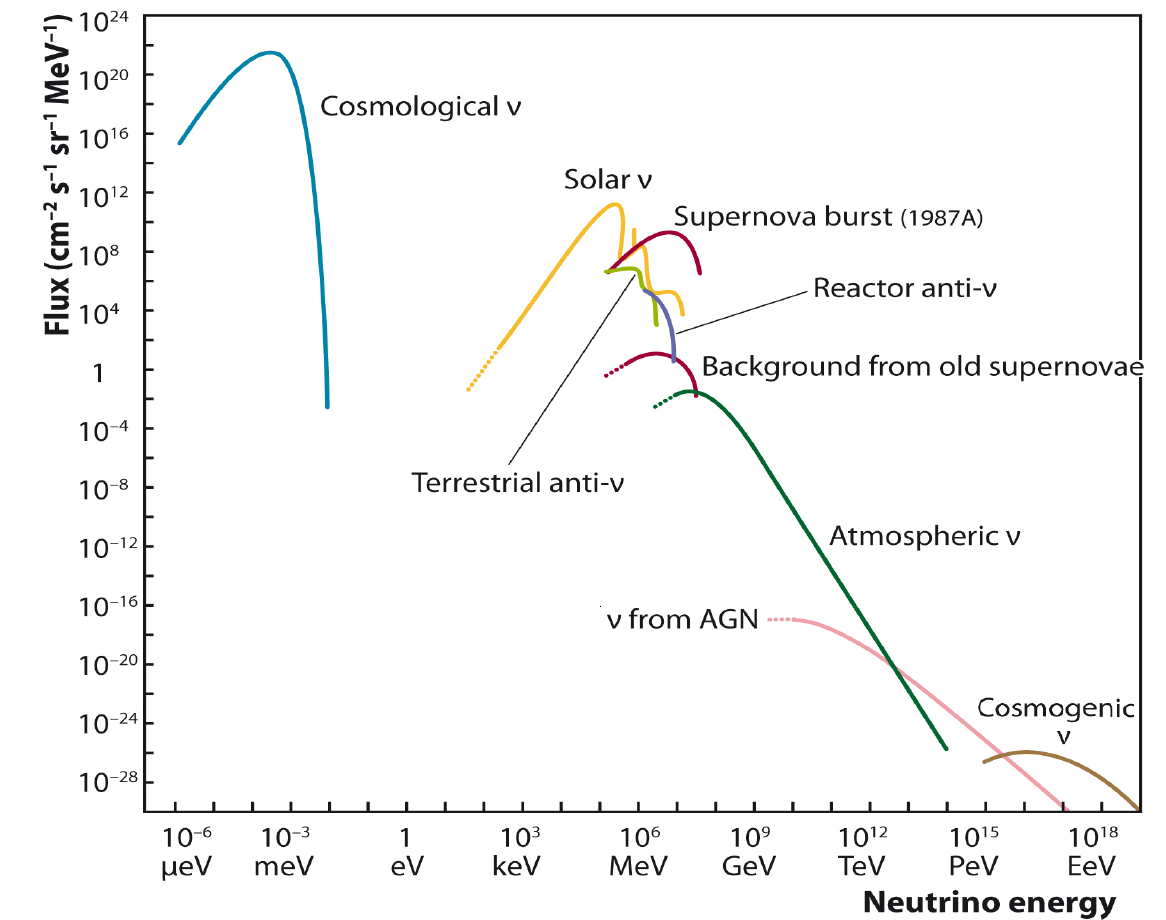
\includegraphics{./figures/nu_phenomenology/all-nu-spectrum-mod.png}
%     \labfig{nu_spectrum}
% \end{figure}
The concept of the neutrino, initially called the "neutron," was first proposed by Pauli in 1930 \sidecite{Pauli} to explain the observed continuous energy spectrum in the beta decay process. Even 60 years after the first direct detection of neutrinos from nuclear reactors by Cowan and Reines \sidecite{nu_discovery}, neutrinos are still the subject of intense experimental investigation, and many of their fundamental properties remain to be measured. This chapter details fundamental properties of Neutrinos in standard model, their interactions and other properties. Last section shall highlight properties and interactions assuming theories \emph{Beyond Standard Model}.
% Neutrinos are produced by various sources across a very large energy range (see \reffig{nu_spectrum}), including particle accelerators, nuclear reactors, and several natural processes. The largest flux of neutrinos comes from nuclear fusion in the Sun \sidecite{Bahcall} and naturally occurring $\beta$-decay on Earth (the so-called \emph{GeoNeutrinos} or \emph{terrestrial neutrinos}) \sidecite{Krauss}. Historically, a similar flux was briefly observed during the supernova SN1987a in the Large Magellanic Cloud, though it only lasted a few seconds \sidecite{SN1987A_superK,SN1987A_Baksan,SN1987A_IMB}. A more constant, but significantly lower, flux is thought to arise from numerous supernovae throughout the universe \sidecite{Vissani}. High-energy neutrinos, above 1 TeV, originate from either atmospheric or astrophysical sources and are of particular interest for the work presented in this thesis. 
\section{Neutrinos in Standard Model}
\label{sec:sm_nu}
In the Standard Model (SM) of particle physics, neutrinos are fundamental particles characterized as massless, chargeless, and colorless fermions that come in three distinct flavors: electron neutrinos ($\nu_e$), muon neutrinos ($\nu_\mu$), and tau neutrinos ($\nu_\tau$). Neutrinos interact solely via the weak force, which is mediated by the exchange of $W^\pm$ and $Z^0$ bosons, making them highly elusive and difficult to detect in experiments. This weak interaction is responsible for the rare instances where neutrinos can interact with other particles, allowing them to traverse vast distances across the universe almost unhindered. The Standard Model is built upon the conservation of charge, parity, and time reversal symmetry (\emph{CPT symmetry}). Under CPT symmetry, for every left-handed fermion, there exists a corresponding right-handed antiparticle with an opposite charge. However, this symmetry does not necessitate the existence of a right-handed particle state. In the case of neutrinos, the SM originally postulated them as Weyl fermions—particles that have no mass and possess only left-handed components. Consequently, the left-handed neutrino was considered the particle, and the right-handed antineutrino its antiparticle. 


\subsection{Mass and Oscillations}
\label{sec:nu_mass_osc}
The Standard model neutrinos were initially thought to be massless, but when the Homestake experiment measured the flux of solar neutrinos (electron anti-neutrinos ($\bar{\nu}_e$)) \sidecite{homestake}, which was one third of what the solar models predicted \sidecite{Bethe39}, many theories of neutrino oscillations\footnote{Technically, this in itself hints towards Physics beyond standard model as in order for neutrinos to oscillate between flavours, at least two of the three flavours must have non-zero mass.} were put forward to explain why the deficit was observed. The Sudbury Neutrino Observatory later confirmed neutrino oscillations by detecting all neutrino flavors through neutral-current interactions \sidecite{Ahmad_2001}, aligning with solar models. Additional confirmation came from the Super-Kamiokande detector measurement, which observed the disappearance of atmospheric muon neutrinos after passing through the Earth \sidecite{SuperK_osc}, further substantiating neutrino oscillations. 

The weak interactions violate parity symmetry, as shown by Chien-Shiung Wu in 1956 through her study of the beta decay of cobalt-60 nuclei \sidecite{Wu}. This discovery revealed that only left-handed particles and right-handed antiparticles take part in weak interactions, violating CPT symmetry. This finding also raised the possibility that neutrinos might have right-handed particles and left-handed antiparticles, but they are not observed due to the weak interaction's non-preference. In the Standard Model, fermions acquire mass through interactions with the Higgs field, which requires both left-handed and right-handed states. However, no right-handed neutrinos have been observed, leading to speculation about how neutrinos obtain their mass. One possible explanation is the introduction of a right-handed neutrino that interacts with the Higgs field, resulting in \textbf{Dirac neutrinos}, which maintain lepton number conservation. Alternatively, the right-handed state could be identified as the antiparticle of the left-handed state, leading to \textbf{Majorana neutrinos}, where the neutrino is its own antiparticle, without imposing lepton number conservation.

Although oscillations have confirmed that neutrinos are not massless, the precise values are still uncertain, with only upper limits currently known. Direct measurements derived from the beta decay energy spectrum indicate that the effective electron neutrino mass is likely less than 0.8eV \sidecite{katrin}. Indirect astrophysical and cosmological observations provide an even more stringent constraint, suggesting that the sum of all neutrino masses ($\sum{{m}_{\nu}})$ is below 0.12 eV \sidecite{cosmologymass}. 

\subsubsection*{Neutrino Oscillations in Vacuum}
\label{sec:nu_osc_vacuum}
It was first suggested by Bruno Pontecorvo that neutrino oscillations would be possible if neutrinos had mass \sidecite{Pontecorvo}. In accordance with this theory, when a neutrino is produced in a weak interaction, it is in a flavor eigenstate denoted as $\nu_{\alpha}$. However, this flavor eigenstate is actually a superposition of the neutrino mass eigenstates $\nu_{i}$, which are the true eigenstates of the Hamiltonian governing neutrino propagation. Mathematically, the flavor eigenstate $\nu_{\alpha}$ can be expressed as:
\begin{equation}\label{eq:flav_to_mass}
        |\nu_{\alpha}\rangle = \sum_{j=1}^{N_{\nu}} U_{\alpha j}^* |\nu_j\rangle
\end{equation}
\marginnote{
        \begin{kaobox}
        The number of active neutrinos, denoted as $N_{\nu}$, is determined to be 3 based on experimental observations. This was done by measuring the decay width of the $Z^0$ boson at LEP using electron-positron collisions at the resonance energy of the $Z^0$ particle \cite{Z_decay}. The result, $N_{\nu} = 2.984\pm  0.008$, is consistent with the existing understanding of 3 active neutrino flavors. 
        \end{kaobox}}
where, where $N_{\nu}$  represents the number of neutrino species, here assumed to be 3 \sidecite{Z_decay}, and $U$ is the Pontecorvo-Maki-Nakagawa-Sakata (PMNS) mixing matrix (analogous to CKM Matrix in quark sector). This matrix encapsulates the probabilities of different mass eigenstates contributing to a particular flavor eigenstate. 
The PMNS mixing matrix $U^*$ can be written as a product of rotation matrices and phase factors:

\begin{equation*}\label{eq:pmns}
U^{*} = \begin{pmatrix}
1 & 0 & 0 \\
0 & c_{23} & s_{23} \\
0 & -s_{23} & c_{23} 
\end{pmatrix}
\begin{pmatrix}
c_{13} & 0 & s_{13} e^{i\delta} \\
0 & 1 & 0 \\
-s_{13} e^{i\delta} & 0 & c_{13} 
\end{pmatrix}
\begin{pmatrix}
c_{12} & s_{12} & 0 \\
-s_{12} & c_{12} & 0 \\
0 & 0 & 1
\end{pmatrix}
\begin{pmatrix}
e^{i\alpha_1} & 0 & 0 \\
0 & e^{i\alpha_2} & 0 \\
0 & 0 & 1
\end{pmatrix},
\end{equation*}

where $c_{ij} = \cos\theta_{ij}$ and $s_{ij} = \sin\theta_{ij}$ represent the mixing angles between different neutrino flavors, $\delta$ is the Dirac CP-violating phase, and $\alpha_1$ and $\alpha_2$ are the Majorana phases. These parameters control the extent and nature of neutrino mixing, ultimately determining how likely a neutrino produced as one flavor is to be detected as another after propagating a certain distance. The mixing parameters of the matrix have been extensively measured through various experiments, including studies of atmospheric neutrinos in IceCube \sidecite{IceCube_atm_numixing}. The latest fit-results of a global fit (NuFIT 5.3) \sidecite{Esteban:2020cvm} using data of many experiments is shown in \reftab{mixing_parameters}. While the values of $\Delta m^2_{ij}$ are well determined, the sign of the mass-squared difference is only known for $\Delta m^2_{12}$, resulting in two possible mass orderings. In the normal ordering (NO), the masses follow $m_1 < m_2 < m_3$, while in the inverted ordering (IO), the hierarchy is $m_3 < m_1 < m_2$. The data indicate that the strongest mixing occurs between $\nu_1$ and $\nu_2$, as well as between $\nu_2$ and $\nu_3$. The mass ordering and the CP-violating phase $\delta_{\text{CP}}$ remain largely unconstrained, but recent global fits suggest a preference for $\delta_{\text{CP}} \neq 0$ and indicate that the normal ordering is favored over the inverted ordering.

\begin{table}[h!]
        \caption{The oscillation parameters determined from the NuFIT 5.3 (2024) global analysis \cite{Esteban:2020cvm}. Results are presented for the assumption of a normal mass hierarchy and an inverted mass hierarchy. Here $\Delta m^2_{3l}$ represents $\Delta m^2_{31}$ for the normal hierarchy or $\Delta m^2_{32}$ for the inverted hierarchy. The parameters are shown for globalfit values without SuperKamiokande's atmospheric data, for more details see \url{http://www.nu-fit.org}}
        \labtab{mixing_parameters}
        {\renewcommand{\arraystretch}{1.4}
        \begin{tabular}{LLL}
            \hline
            \hline
             & \mathrm{Normal \, Ordering} & \mathrm{Inverted \, Ordering}\\
            \hline
            \theta_{12} [^{\circ}] &33.66_{-0.70}^{+0.73}&33.67_{-0.71}^{+0.73}\\
            \theta_{23} [^{\circ}] &49.1_{-1.3}^{+1}&49.5_{-1.2}^{+0.9}\\
            \theta_{13} [^{\circ}] &8.54_{-0.11}^{+0.11}&8.57_{-0.11}^{+0.11}\\
            \delta_{\mathrm{CP}} [^{\circ}] &197_{-25}^{+41}&286_{-32}^{+27}\\
            \Delta m^2_{21}[10^{-5}\mathrm{eV}^2]&7.41_{-0.20}^{+0.21}&7.41_{-0.20}^{+0.21}\\
            \Delta m^2_{3l}[10^{-5}\mathrm{eV}^2]&+2.51_{-0.027}^{+0.027}&-2.498_{-0.024}^{+0.032}\\
            \hline
            \hline
\end{tabular}}
\end{table}
In addition to the assumed three neutrino species, throughout the remainder of this discussion (as derived in \sidecite{Osc_derivation}) of neutrino oscillation, neutrinos are assumed to be Dirac particles and hence the fourth matrix in Equation \ref{eq:pmns}, containing Majorana Phases is dropped\sidenote{Additionally, throughout the derivation, Natural units are used, i.e $\hbar=c=1$. Hence, mass is in units of energy and time is given in the units of distance.} 

After traveling a distance \(L\) (or, equivalently for relativistic neutrinos, time \(t\)), a neutrino originally produced with a flavor \(\alpha\) evolves as follows:

\begin{equation}\labeq{}
|\nu_\alpha(t)\rangle = \sum_{j=1}^{n} U_{\alpha j}^* |\nu_j(t)\rangle,
\end{equation}

Using an approximation that the neutrino state is a plane wave $|\nu_j(t)\rangle = e^{-iE_j t} |\nu_j(0)\rangle$, and assuming neutrinos are relativistic, The transition probability of a neutrino initially produced with flavour $\nu_{\alpha}$ to $\nu_{\beta}$ after time $t$ can be given as,
\marginnote{
        \begin{kaobox}
        In Equation~\ref{eq:main_probability}, the term $\frac{\Delta m_{jk}^2 L}{2E}$ is a replacement for $(E_j-E_k)t$. In ultra-relativistic limits, if all mass eigenstates have the same momentum, one can approximately express the energy in terms of the mass of each state as,
        \begin{equation}\label{eq:mass_limit}
                E_j = \sqrt{p_j^2 + m_j^2} \approx E + \frac{m_j^2}{2E}.
                \end{equation}
         Also, by assuming all neutrinos are travelling approximately at the speed of light $c$, time $t$ can be expressed in terms of propagation length $L$.
        \end{kaobox}}
\begin{equation}\label{eq:oscillation}
        \begin{split}
                P(\nu_\alpha \rightarrow \nu_\beta) &= |\langle \nu_\beta | \nu_\alpha(t) \rangle|^2 \\
                &=  \sum_{j,k} U_{\alpha j}^* U_{\beta j} U_{\alpha k} U_{\beta k}^* e^{-i(E_{j}-E_{k})t} 
        \end{split}
\end{equation}
            

Using the orthogonality relation $\langle \nu_i(0) | \nu_j(0) \rangle = \delta_{ij}$ of the mass eigenstates, the transition probability becomes:

\begin{equation}\label{eq:main_probability}
P(\nu_\alpha \rightarrow \nu_\beta) \approx \sum_{j,k} U_{\alpha j}^* U_{\beta j} U_{\alpha k} U_{\beta k}^* e^{-i \frac{\Delta m_{jk}^2 L}{2E}},
\end{equation}

The mass-squared difference between the mass eigenstates j and k, denoted as $\Delta m_{jk}^2 = m_j^2 - m_k^2$, is calculated as the difference between $m_j^2$ and $m_k^2$. The probability of flavor transition is a periodic function of the distance L between the source and the detector and is influenced by the mass-squared differences and the neutrino energy. 

\marginnote{\begin{kaobox}
        The transition probability derived in Equation~\ref{eq:twoflavour_transition} has a period with the oscillation length ($L_{\mathrm{osc}}$) determined by the neutrino energy ($E_{\nu}$) and mass difference ($\Delta m^2$) as,
        \begin{equation}\label{eq:twoflav}
                L_{\mathrm{osc}} = \frac{4 \pi E_{\nu}}{\Delta m^2}
        \end{equation}
        and the amplitude is proportional to the mixing angle. From Equation ~\ref{eq:twoflav} for an experiment to be sensitive to a specific value of $\Delta m^2$, it must be configured so that $E/L \approx \Delta m^2$. For example, to measure the parameters $\theta_{23}$ and $\Delta m^2_{32}$, an $L/E$ value of approximately 500 km/GeV is required, which is typical for atmospheric neutrino studies. To probe the parameters $\theta_{12}$ and $\Delta m^2_{12}$, the appropriate $L/E$ would be around 15,000 km/GeV, as seen in solar neutrino experiments. The distance between the neutrino sources and detector, is usually reffered to as \emph{baseline} of the experiment
\end{kaobox}}

In most scenarios, neutrino oscillations can be approximated by two-flavor mixing due to the suppression of three-flavor mixing effects by the small value of $\theta_{13}$ and the large hierarchy between the two mass-squared splittings, where $\Delta m_{21}^2 \ll \Delta m_{32}^2$. As a result, the problem is often simplified to two-flavor oscillations. The transition probability exhibits an oscillatory behavior, hence the name. If $L \gg L_{\mathrm{osc}}$, the oscillating phase completes many cycles before detection and is averaged to 1/2., \emph{Neutrino Oscillations}.

In the simplest case of two-flavor mixing, the mixing matrix depends on just one mixing angle, and there is only one relevant mass-squared difference. The probability\footnote{The probability is the same for neutrinos and antineutrinos.} that a neutrino $\nu_{\alpha}$ with energy $E_{\nu}$ oscillates into a neutrino $\nu_{\beta}$ after traveling a distance L (the so-called \emph{transition probability}) is given by:

\begin{equation}\label{eq:twoflavour_transition}
P(\nu_\alpha \rightarrow \nu_\beta) = \sin^2(2\theta) \sin^2\left(\frac{\Delta m^2 L}{4 E_\nu}\right), \quad \alpha \neq \beta.
\end{equation}

As opposed to the case where the probability that a neutrino $\nu_{\alpha}$ with energy $E_{\nu}$ after traveling a distance L is still measured in state of $\nu_{\alpha}$ (the so-called \emph{survival probability}) is given by:

\begin{equation}\label{eq:twoflavour_survival}
        P(\nu_\alpha \rightarrow \nu_\alpha) = 1-\sin^2(2\theta) \sin^2\left(\frac{\Delta m^2 L}{4 E_\nu}\right), \quad \alpha = \beta.
\end{equation}

\subsubsection*{Neutrino Oscillations in Matter}
\label{sec:nu_osc_matter}
The discussion so far has assumed that neutrinos travel through a vacuum. However, when neutrinos travel through matter, their interactions with the medium alter their properties. This happens because of coherent forward scattering on electrons and nucleons, which modifies the amplitude of their propagation. Initially the idea that the oscillation parameters of neutrinos are altered in matter was coined by Lincoln Wolfenstein's \sidecite{MSW1,MSW2}. In 1985, Stanislav Mikheyev and Alexei Smirnov predicted that a gradual decrease in the density of matter can resonantly enhance neutrino mixing \sidecite{MSW3}. 

In the presence of matter, the Hamiltonian of the system changes by experiencing an \emph{Effective Potential} ($V_{\mathrm{eff}}$). As a result, the mass eigenstates and eigenvalues of  this effective hamiltonian changes, meaning that neutrinos in matter now have a different effective mass than they did in a vacuum. Since neutrino oscillations depend on the squared mass difference of the neutrinos, neutrino oscillations experience different dynamics than they did in a vacuum. This theory formed basis to solve the solar neutrino puzzle, where observed deficit of neutrino fluxes could only be explained by not only neutrino oscillations but also the matter effects that the produced neutrinos in the sun core goes through while reaching the surface, and later crossing the threshold of higher matter density to vacuum \sidecite{MSW4,MSW5}. 

\subsection{Interactions}
\label{sec:nu_interactions}
In the Standard Model, neutrinos only interact through the weak interaction, which is mediated by the exchange of the $W^{\pm}$ and $Z^0$ bosons. These bosons have masses of $M_{W^{\pm}}=80$ GeV  and $M_{Z^0}=91$ GeV \sidecite{PDG_2024}. The massiveness of these bosons contribute to the weakness of the interaction in normal conditions. Processes involving the W-boson are referred to as charged-current (CC) processes, while those involving the Z-boson are called neutral-current (NC) processes Neutrinos interact with charged leptons ($e^{\pm}$, $\mu^{\pm}$, $\tau^{\pm}$) through scattering processes and are produced in the decays of unstable charged leptons such as $\mu^{\pm}$ and $\tau^{\pm}$. They also interact with quarks, both in bound states (e.g., neutrons, protons, pions) through neutrino-nucleon scattering, and as individual quarks (partons) through deep inelastic scattering

This section will cover the general properties of neutrino interactions, focusing on their cross-sections across various energy scales. Later subsections will explore high-energy interaction processes, which are important for understanding neutrino behavior in extreme environments and are relevant to the analysis presented in this thesis.

\subsubsection*{Interaction Cross-Sections}
\label{sec:xsec}
Neutrino interactions can exhibit a wide range of behaviors \sidecite{xsec_overview} depending on the energy at which they occur and whether the interaction involves a neutrino or an antineutrino, as shown in \reffig{total_xsec}. 

\begin{figure*}[h!]
        \begin{subfigure}[h]{0.7\textwidth}
            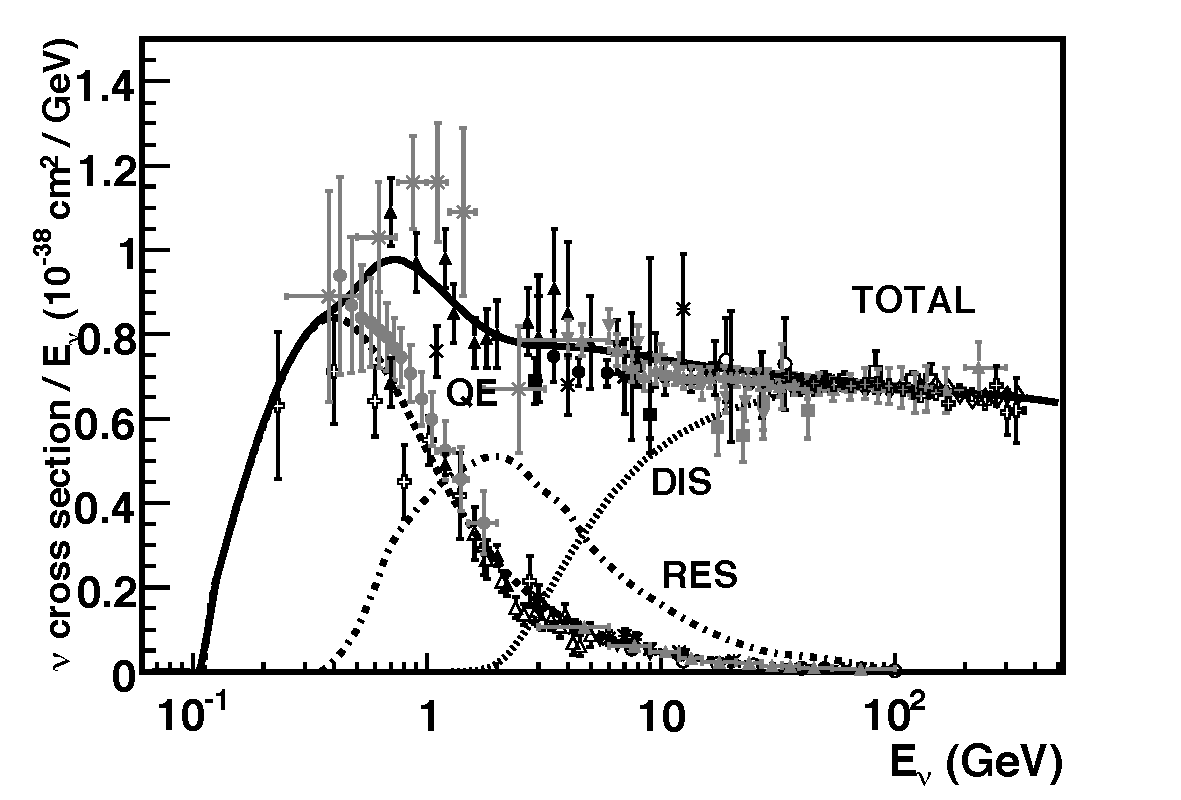
\includegraphics{./figures/nu_phenomenology/cc_inclusive_nu.pdf}
        \end{subfigure}
        \hfill
        \begin{subfigure}[h]{0.7\textwidth}
            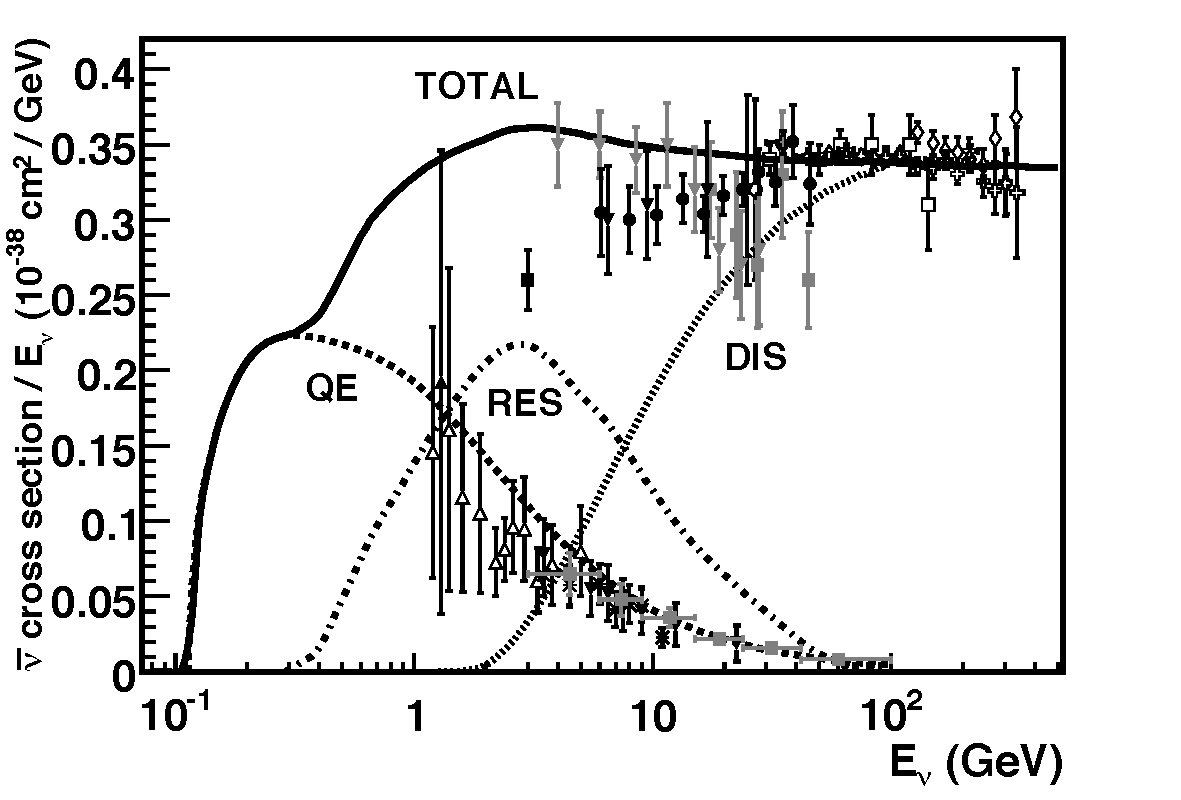
\includegraphics{./figures/nu_phenomenology/cc_inclusive_nubar.pdf}
        \end{subfigure}
        
        \caption{Total cross-sections for neutrinos (left) and antineutrinos (right) per nucleon in charged-current interactions (for an isoscalar target) divided by neutrino energy as a function of neutrino energy. Figure taken from \cite{xsec_overview} }
        \labfig{total_xsec}
\end{figure*}

\marginnote{\begin{kaobox}[title=\textbf{Inverse Beta Decay (IBD)}]
       In IBD, $\bar{\nu_{e}}$ interacts with a proton, producing a $e^+$ and a neutron. The $\bar{\nu_{e}}$ must have a minimum kinetic energy of 1.806 MeV to initiate the reaction. This is due to the mass difference between the reactants and products. The positron receives most of the antineutrino's energy due to its smaller mass compared to the neutron.
        \begin{equation}\label{eq:IBD}
                 \bar{\nu}_e + p \rightarrow e^+ + n 
        \end{equation}
\end{kaobox}
}
At low energies, typically up to around 1 MeV, neutrino interactions are dominated by scattering off leptons and nuclei, both in charged and neutral forms. Two notable processes in this energy range are \textbf{coherent scattering} and \textbf{Neutrino Capture on Radioactive Nuclei}. These low-energy interactions can be described through electroweak theory, where the neutrino engages in two-body scattering processes. As the neutrino energy increases, it becomes possible to probe the target nucleus at progressively smaller length scales. While coherent scattering treats the nucleus as a unified structure, higher-energy neutrinos can resolve individual nucleons. One significant low-energy process is the Inverse Beta Decay (IBD). This process has been extensively studied in several experiments such as KamLAND \sidecite{KamLAND_osc} and Daya Bay \sidecite{DayaBay}, which measures neutrino oscillations using  anti-neutrinos produced in fission nuclear reactors, typically probing energies up to around 10 MeV.

As the energy increases to the GeV range, neutrinos primarily interact through \textbf{quasi-elastic scattering} and \textbf{resonance production}. In quasi-elastic scattering, neutrinos interact with nucleons, producing charged leptons without breaking apart the nucleon. At slightly higher energies, resonance production becomes a crucial interaction mode. In this case, neutrinos excite the target nucleon into resonance states, such as $\Delta$ or $N^*$, which subsequently decay into various final states, yielding combinations of nucleons and mesons. The energy range of around 10 GeV is often called \emph{the transition region} because it separates quasi-elastic scattering, where the target is a nucleon, from \textbf{ the deep inelastic scattering (DIS)}, where the target is a quark (or \emph{parton}) within the nucleon. As shown in \reffig{total_xsec}, above this transition region ($> 100$ GeV), the total cross-section exhibits an almost linear relationship with neutrino energy and DIS becomes the dominant process of all neutrino interactions. This scaling behavior, as predicted by the quark-parton model \sidecite{parton}, assumes point-like scattering off quarks. However, these assumptions are not valid at lower neutrino energies, where lower momentum transfers have a greater impact on the interaction dynamics \sidecite{xsec_overview}. Since this energy range is critical for high-energy neutrino interactions in IceCube, especially for the analysis presented in this thesis, only DIS (and other relavnt processes at this energy, see Section \ref{sec:glashow}) process shall be discussed in more detail. 

\subsubsection*{Neutrino-Nucleon Deep Inelastic Scattering}
\label{sec:DIS}
\begin{marginfigure}
\centering
\begin{tikzpicture}
\begin{feynman}
        \def\flen{1.5}
        \def\boslen{1.4}
        \def\fangle{45}

        
        

        \vertex (v1)  at (0, \boslen);
        \vertex (i1) at ($(v1) + (180-\fangle:\flen)$) {$\barp{\nu_{l}}$};
        \vertex (f1) at ($(v1) + (\fangle:\flen)$) {$\mathcal{l}^{\pm}$};

        \vertex (v2)  at (0, 0) ;
        \vertex (i2) at ($(v2) + (\fangle-180:\flen)$) {$N$};
        \vertex (f2) at ($(v2) + (-\fangle:\flen)$) {$X$};

        \diagram* {
        (i1) -- [fermion] (v1) -- [fermion] (f1),
        (v1) -- [boson, edge label=$W^{\mp}$] (v2),
        (i2) -- [fermion] (v2) -- [fermion] (f2)
        };
\end{feynman}
\end{tikzpicture}
\caption{Feynman diagram of Neutrino-Nucleon DIS via CC interaction.}
\labfig{DIS_CC}
\end{marginfigure}
\begin{marginfigure}
\centering
\begin{tikzpicture}
\begin{feynman}
        \def\flen{1.5}
        \def\boslen{1.4}
        \def\fangle{45}

        % in order to get the [dot] to work, we need to add the empty braces
        

        \vertex (v1) at (0, \boslen);
        \vertex (i1) at ($(v1) + (180-\fangle:\flen)$) {$\barp{\nu_{l}}$};
        \vertex (f1) at ($(v1) + (\fangle:\flen)$) {$N$};

        \vertex (v2) at (0, 0);
        \vertex (i2) at ($(v2) + (\fangle-180:\flen)$) {$\barp{\nu_{l}}$};
        \vertex (f2) at ($(v2) + (-\fangle:\flen)$) {$N'$};

        \diagram* {
        (i1) -- [fermion] (v1) -- [fermion] (f1),
        (v1) -- [boson, edge label=$Z^{0}$] (v2),
        (i2) -- [fermion] (v2) -- [fermion] (f2)
        };
\end{feynman}
\end{tikzpicture}
\caption{Feynman diagram of Neutrino-Nucleon DIS via NC interaction.}
\labfig{DIS_NC}
\end{marginfigure}
In Deep Inelastic Scattering (DIS), neutrinos interact with quarks inside nucleons, breaking them apart and producing a cascade of particles. In this high-energy regime, the neutrino can be seen as scattering off individual partons, but a scattered parton cannot remain free for long. It quickly creates a jet of hadrons through pair production, a process known as hadronization or fragmentation. Both charged-current (CC) and neutral-current (NC) interactions can occur this way, resulting in either an outgoing charged lepton or neutrino. Feynman diagrams of CC and NC interactions for neutrinos are shown in \reffig{DIS_CC} and \reffig{DIS_NC} respectively, with their corresponding reactions in Equation~\ref{eq:CC} and Equation~\ref{eq:NC}. The most general form of the differential neutrino-nucleon cross section for a CC interaction, involving an incoming neutrino with initial four momentum $k_1$, scattering with a target nucleon with four-momentum $p$, resulting in an outgoing lepton with four-momentum $k_2$, and a virtual gauge boson with four-momentum transfer q=$k_1-k_2$, can be expressed as:

\begin{equation}\label{eq:DIS_xsec_formula}
        \frac{d^2\sigma}{dx,dy} = \frac{G_F^2m_N E_\nu}{\pi} \left(\frac{{M_W^2}^2}{{Q^2}+{M_W^2}^2}\right)^2 \left[ q(x,Q^2) + (1-y)^2 \bar{q}(x,Q^2) \right] 
\end{equation}

\marginnote{
        %\begin{kaobox}[title=\textbf{Deep Inelastic Scattering of Neutrino-Nucleon}]
        \textbf{Charged Current Interaction}\\ (see feynman diagram \reffig{DIS_CC})
        \begin{equation}\label{eq:CC}
                \barp{\nu_{l}} + N \rightarrow \mathcal{l}^{\pm} + X
        \end{equation}
        \textbf{Neutral Current Interaction}\\ (see feynman diagram \reffig{DIS_NC})
        \begin{equation}\label{eq:NC}
                \barp{\nu_{l}} + N \rightarrow \barp{\nu_{l}} + X
       \end{equation}
       Here, $N$ is a nucleon, $\barp{\nu_{l}}$ is the $\nu$/$\bar{\nu}$ of flavour $l$ and X is hadronic particle shower.
        %\end{kaobox}
        }

where, $G_F$ represents the Fermi constant, $m_N$ is the nucleon mass, $E_{\nu}$ is the energy of the incoming neutrino, and $M_W$ represents the W-boson mass. The invariant momentum transfer of the scattering process is $Q^2 = -q^2$. \textbf{The Bjorken scaling variable}, 
\begin{equation}\label{eq:bjorkenx}
        x = \frac{Q^2}{p.q}
\end{equation}
represents the fraction of the nucleon's momentum carried by the scattered quark, while \textbf{the inelasticity variable}, 
\begin{equation}\label{eq:inelasticity}
        y = \frac{p.q}{p.k_1}=\frac{E_{hadron}}{E_{\nu}}
\end{equation}
measures the amount of energy transferred to the hadronic system X. The parton distribution functions (PDFs), $q(x, Q^2)$ and $\bar{q}(x, Q^2)$, represent the probability density of a quark or antiquark, respectively, to have a momentum fraction $x$ of the nucleon at the energy scale $Q^2$ of the interaction. 

\begin{figure}[h!]
        \caption{The deep inelastic scattering cross-sections for neutrino and antineutrinos are shown for both CC and NC interactions on an isoscalar target. Glashow resonance peak of $\bar{\nu_e}$ interacting with $e$ is also visible at 6.3 PeV. Figure taken from \cite{DIS_xsec_plot}}
        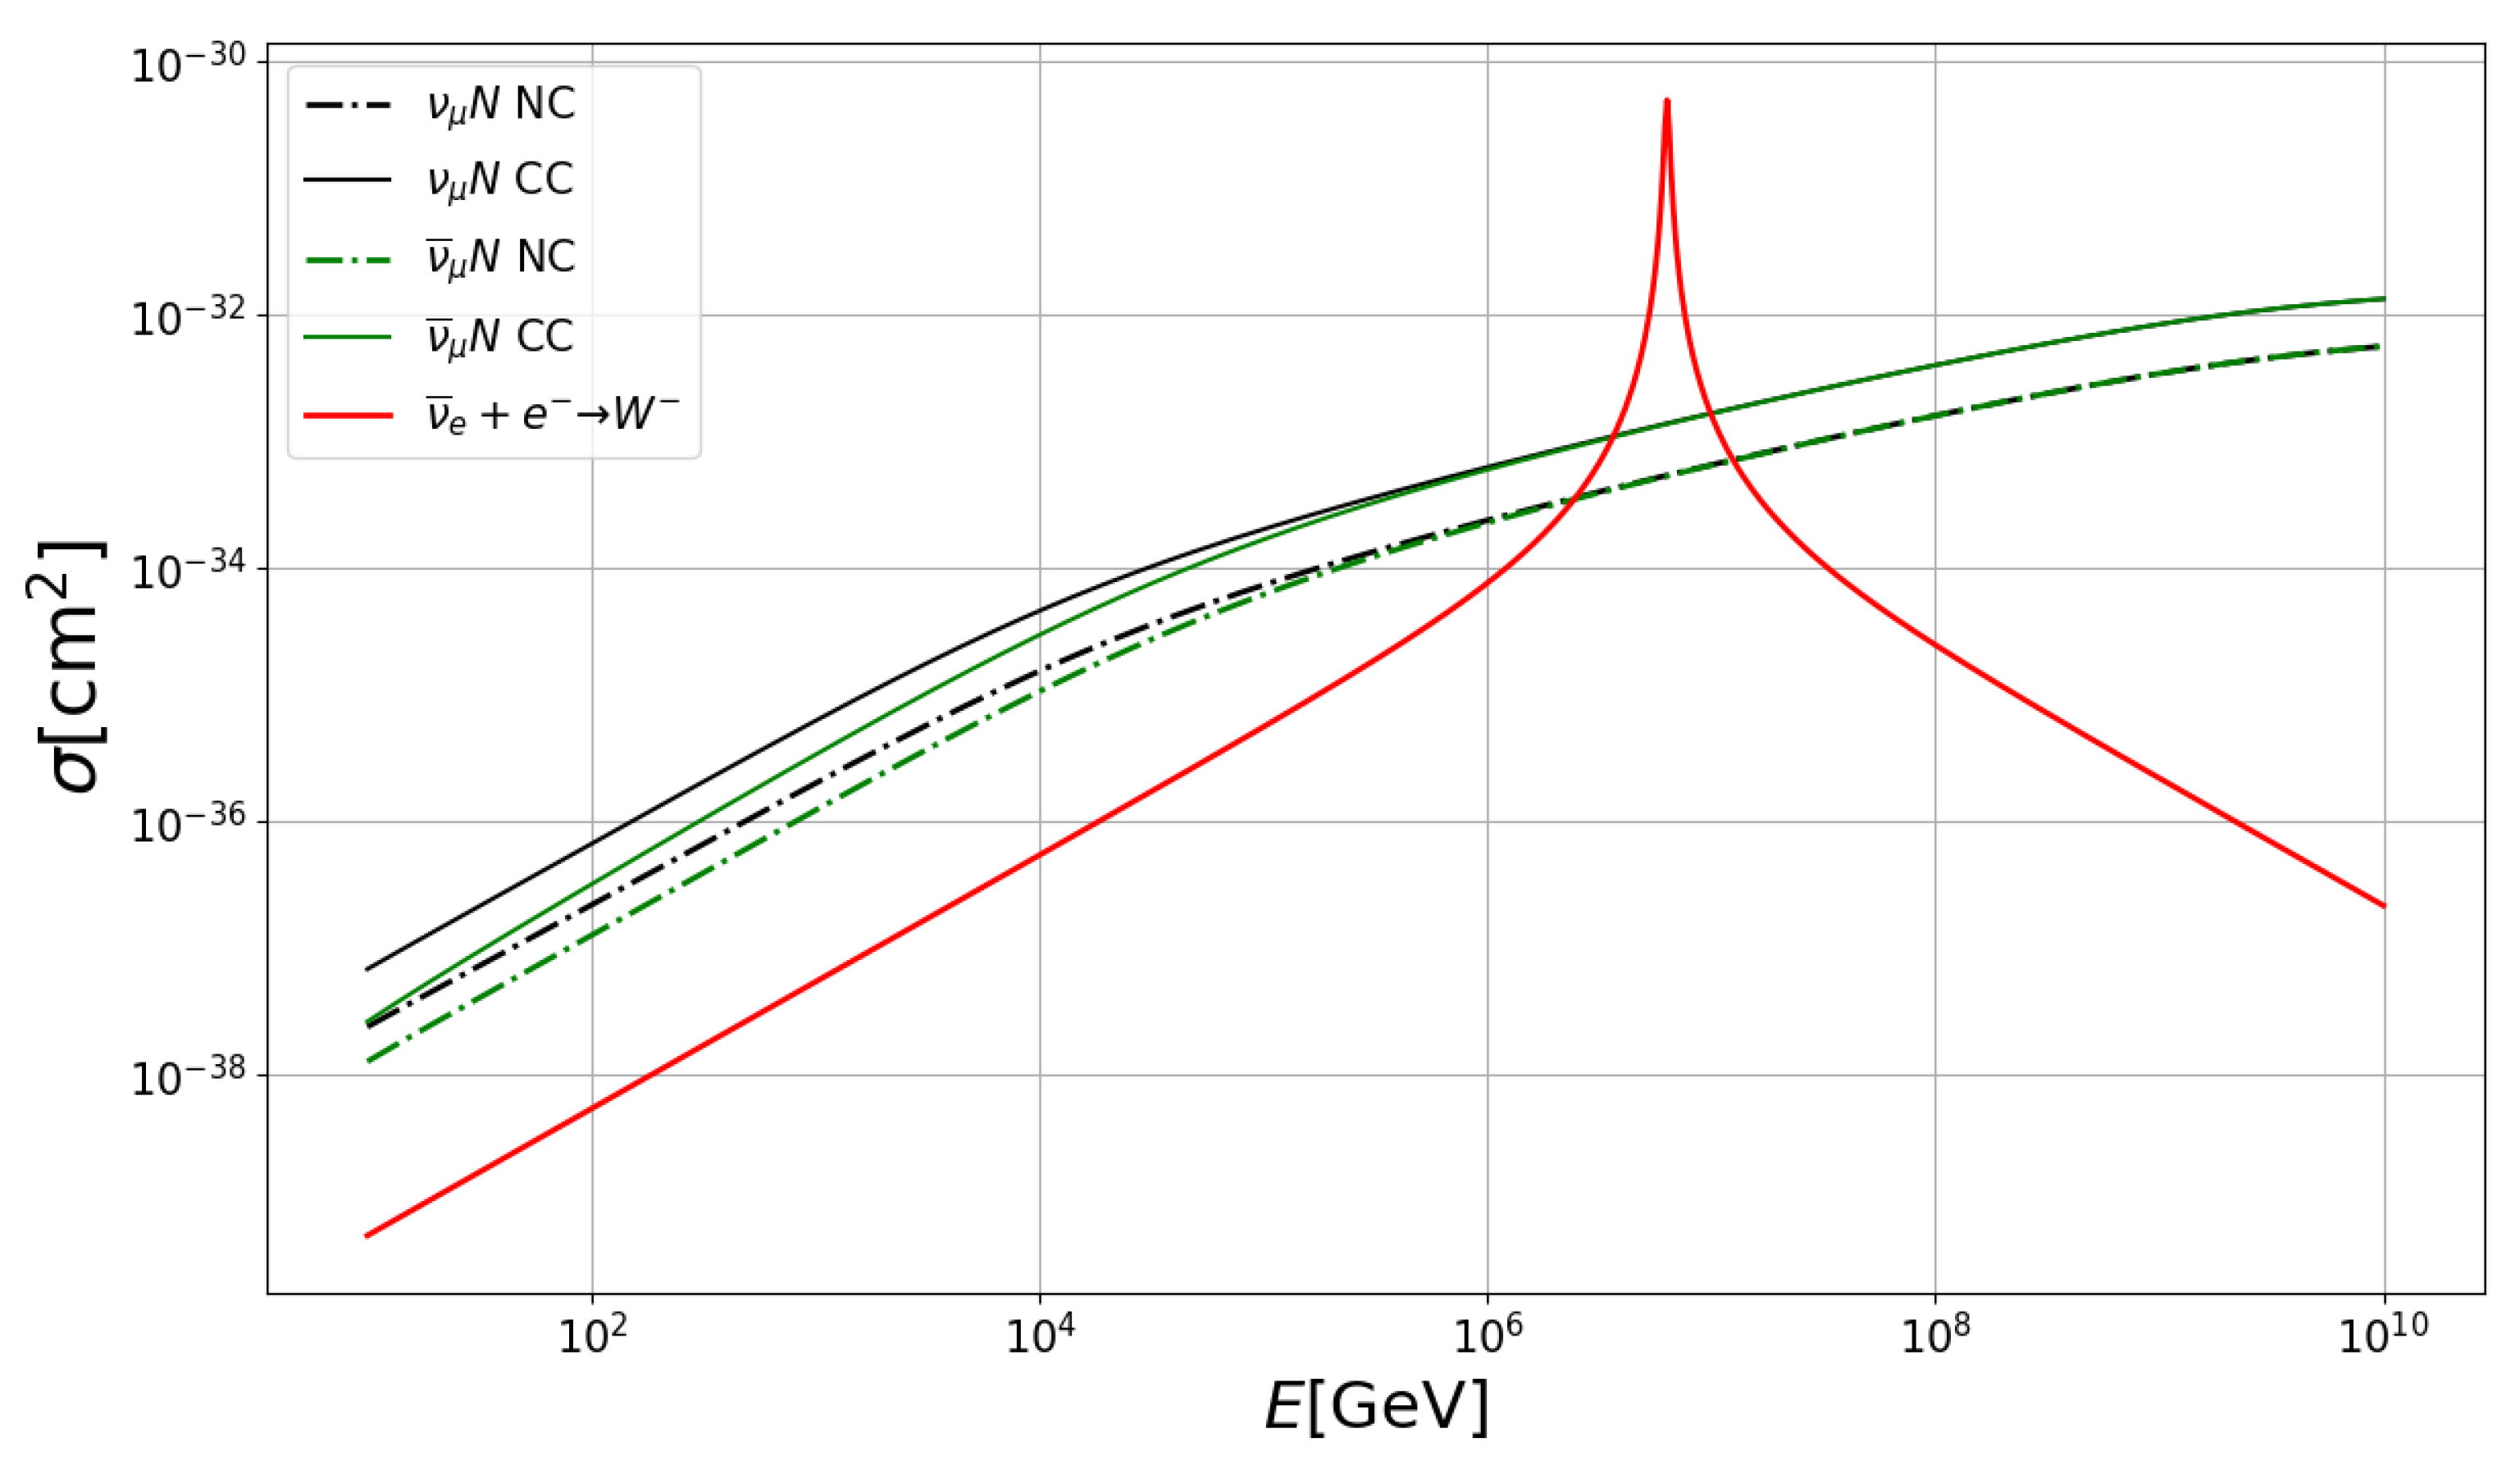
\includegraphics{./figures/nu_phenomenology/xsec_DIS.png}
        \labfig{xsec_DIS}
\end{figure}
A key feature of all structure functions is that they become nearly independent of $Q^2$ in the limit $Q^2 \rightarrow \infty$, meaning cross-section starts to scale linearly with neutrino energy $E_{\nu}$ for up-to $\sim 1$ PeV as shown in \reffig{xsec_DIS}. This property, known as Bjorken scaling, was crucial in developing the parton model for deep inelastic scattering \sidecite{Bjorken_scaling}.  The \reffig{xsec_DIS} illustrates the contributions of CC and NC interactions for both neutrinos and antineutrinos separately. It is evident that the CC cross-section is generally larger than the NC cross-section due to the stronger coupling of the W-boson compared to the Z-boson. At higher energies (> few PeVs), the propagation term from the interaction vertex is no longer dominated by the $W$-$Z$ boson mass. As a result, the cross-section no longer grows linearly with neutrino energy. Moreover, the $(1 - y)^2$ (see second term in bracket of Equation~\ref{eq:DIS_xsec_formula}) suppression that typically allows distinction between neutrino and anti-neutrino interactions is much less pronounced, making the two cross-sections nearly identical \sidecite{Gandhi_1998}.

The calculation of neutrino DIS in the energy range of interest for IceCube has been carried out by Cooper-Sarkar, Mertsch, and Sarkar (CSMS) in 2011 and is the standard that will be used throughout this work to produce neutrino simulation (see Section \ref{sec:mc_sim}) and also to include inelasticity parameter in the forward folding fit (see Section \ref{sec:params}) \sidecite{CSMS}. However, updated cross-section calculations now exists, that takes into account final state radiations (FSR) \cite{xsec_alfonso} and  uses updated parton distribution functions \cite{CT18}. In particular, corrections in visible energy of Glashow events due to FSR were taken into account by introducing a correction in simulation event weight (see Section \ref{sec:glashow_correction} for details). In the last decade, several studies have used different event samples at higher energies to measure the total\footnote{total cross-sections are inclusive of CC and NC interactions.} DIS cross-section in the multi-TeV energy range at IceCube \sidecite{xsec_Sandy, xsec_HESE7}.

\subsubsection*{Glashow Resonance}
\label{sec:glashow}
Neutrinos typically interact with atomic electrons in a detector medium less frequently than with nucleons due to the smaller mass of the electron \sidecite{xsec_overview}. However, an exception occurs during the resonant enhancement of the $\bar{\nu}_e e^-$ scattering cross- section, known as \textbf{the Glashow resonance}. This happens when the center-of-mass energy matches the mass of the $W$-boson. The resonance occurs at an antineutrino energy of $E_{\bar{\nu}} = \frac{M_W^2}{2m_e} \approx 6.3$ PeV, where $m_e$ is the electron mass (see \reffig{xsec_DIS}). Produced W boson, deacays into hadrons/lepton creating a particle shower at around 6 PeV energy. Sheldon Glashow first proposed this phenomenon in 1960 as a method to detect the $W$-boson \sidecite{glashow}. Due to experimental limitations, such high-energy events were not observed for many years. However, the IceCube Neutrino Observatory recently reported detecting a Glashow resonance event, providing the first confirmation of this process \sidecite{glashowic}.

\begin{figure}[h!]
        % \vspace*{4.5cm}
        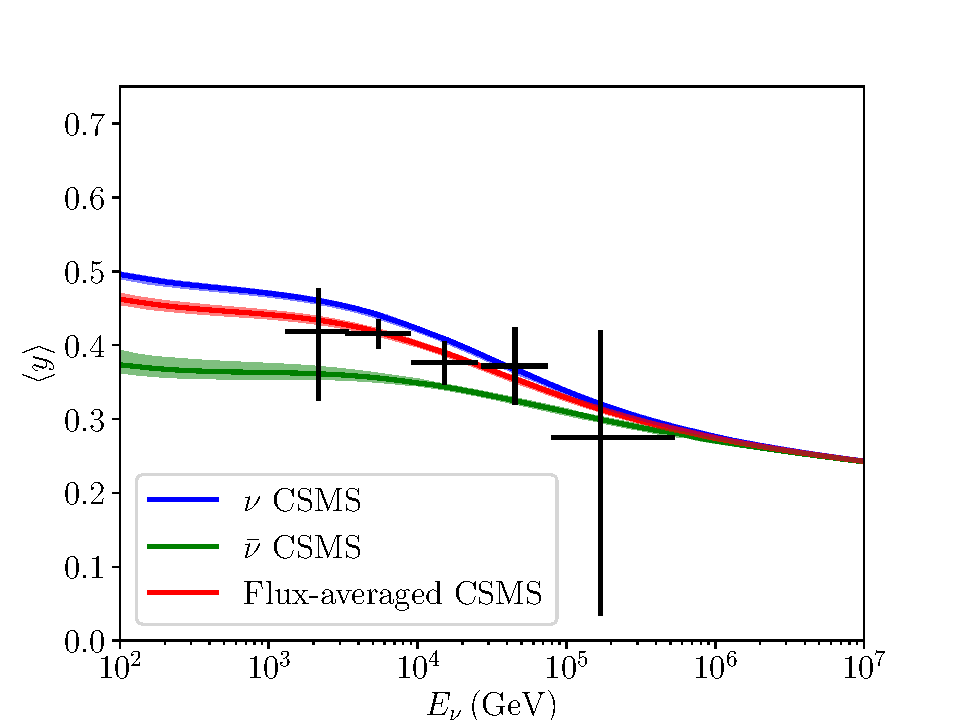
\includegraphics{./figures/nu_phenomenology/split_fit_inel.pdf}
        \caption{The measured mean inelasticity, with error bars indicating 68\% confidence intervals. Predictions from the CSMS model are indicated in blue for $\nu$ and green for $\bar{\nu}$, with theoretical uncertainties shown by the colored bands, along with atmospheric flux-averaged inelasticity in red. Figure taken from \cite{gary_paper}.}
        \labfig{inel_paper}
    \end{figure}

\subsubsection*{Inelasticty}
\label{sec:inelasticity}

Inelasticity, denoted by $y$ as described in Equation \ref{eq:inelasticity}, represents the fraction of the incoming neutrino's energy that is transferred to the hadronic system during deep inelastic scattering (DIS). In neutrino-nucleon DIS, a higher inelasticity corresponds to a larger energy transfer, leading to greater energy deposition in the detector through hadronic showers. Inelasticity can be determined from the kinematics of both the outgoing lepton and the hadronic system. Such a technique was expxloited in an IceCube analysis, to measure inelasticity in TeV range, by using $\nu_{\mu}$-CC events where both interaction vertex (hadronic cascade) and outgoing lepton (\emph{muon track} \sidenote{depending on energy, entire track may or may not be contained within the detector volume, as muon usually deposits some energy along its path and can travel larger distance, possibly leaving the detector, see Section\ref{sec:leptons_inice} for details}) are within the detector \sidecite{gary_paper}. The distinction in inelasticity distribution between $\nu$ and $\bar{\nu}$ (see \reffig{inel_paper}) allows for differentiation between neutrinos and antineutrinos in an event sample. Understanding such an energy dependent inelasticity distribution is crucial for analyzing high-energy neutrino interactions, such as those explored in this thesis, where both hadronic and leptonic energy signatures are used to reconstruct neutrino properties.  


\section{Beyond Standard Model Neutrinos}
\label{sec:bsm}
While the minimum extension used in \ref{sec:nu_mass_osc} provides a framework for describing neutrino oscillations, it also predicts the existence of right-handed neutrinos (or left-handed anti-neutrinos) that do not participate in weak interactions. These non-interacting neutrinos are known as \textbf{\emph{sterile neutrinos}}. Unlike the three active flavors, sterile neutrinos do not contribute to weak interaction processes like $Z^0$ boson decay. Experimental measurements of the $Z^0$ decay width constrain the number of light, active neutrino species (those lighter than the $Z^0$ boson) to 3 \sidecite{Z_decay}. 

Although the three-flavor model is consistent with many observations, anomalies have been observed in several experiments. Radiochemical neutrino experiments \sidecite{radio_chem}, as well as experiments using neutrinos from particle accelerators \sidecite{LSND,MiniBooNE} and anti-neutrinos from nuclear reactors \sidecite{reactor_nu_anamoly}, have reported discrepancies that could be explained by the existence of sterile neutrinos. The simplest theoretical extension to account for these anomalies is the so-called 3+1 model, where one additional sterile neutrino is added to the three active neutrinos. In this model, the PMNS mixing matrix (which describes the mixing between neutrino flavors) is expanded from a $ 3 \times 3$ matrix to a $4 \times 4$ matrix \sidecite{Abazajian:2012ys}. This expanded matrix introduces three new mixing angles ($\theta_{14}, \theta_{24}, \theta_{34} $) and additional CP-violating phases. These additional parameters allow for the mixing of sterile neutrinos with the active ones, potentially explaining the observed experimental anomalies, though further investigation is required to confirm their existence.

Cosmological evidence also provides hints for the existence of sterile neutrinos \sidecite{Abazajian:2017tcc}. The presence of sterile neutrinos could have observable consequences on the evolution of the early universe and on large-scale structure formation. Observations of the cosmic microwave background (CMB) and precise measurements by missions such as WMAP indicate that the number of relativistic species during the early universe, typically expressed as the effective number of neutrino species  $N_{\text{eff}}$, is slightly higher than the expected value of 3 for the three active neutrinos \sidecite{Komatsu_2011}.  This could suggest the presence of additional light particles, such as sterile neutrinos, that contributed to the radiation density in the early universe. Although, another measurement by planck survey is in close agreement with $N_{\text{eff}}=3$ \sidecite{Planck_cosmo}, making the puzzle of such neutrino species even more intriguing.  Moreover, sterile neutrinos could contribute to the dark matter problem \sidecite{kev_dm}. While they are unlikely to account for all dark matter, keV-mass sterile neutrinos are a candidate for \emph{warm dark matter}, a type of dark matter that could impact the formation of structure in the universe on small scales. These cosmological observations, when combined with the experimental anomalies in neutrino oscillation data, make sterile neutrinos an intriguing possibility for both particle physics and cosmology. However, further precision measurements, both in the laboratory and from astrophysical observations, are needed to confirm their existence and determine their exact role in the universe.

In addition to Sterile neutrinos, other exotic phenomena, which are not included in standard model can affect neutrino interaction cross-sections or other fundamental properties assumeed in SM. Such scenarios include interaction of neutrinos with dark matter \sidecite{DarkMatter}, CPT violation \sidecite{CPT_violence} etc. A number of analysis have been made in IceCube to look for sterile neutrinos \sidecite{Trettin2024Search}, other exotic neutral leptons \sidecite{Fischer2024First} and also to look for dark matter signatures \sidecite{IceCube:2023ies} have been made. Although, as it will be discussed in the next chapter, for the analysis presneted in this thesis, as none of these scenraios, when probed to measure flavour fraction of astrophysical neutrinos on earth allows for non-zero tau neutrino fraction \sidecite{overview_bsm_flavour}, hence they are not discussed further in detail, and for the remainder of this thesis, 3 flavour of neutrinos shall be assumed. 
% \setchapterpreamble[u]{\margintoc}
\chapter{Neutrinos in High Energy Universe}
\labch{nu_theory_sources}




\section{Cosmic Rays}

\label{sec:cosmic_rays}

\subsection{Sources}

\subsection{Air Showers}


\section{Cosmic Neutrinos}
\label{sec:cosmic_nu}

\subsection{Sources and Production Mechanisms}

\subsection{Diffuse Fluxes}

\subsection{Flavour Composition}
% \setchapterpreamble[u]{\margintoc}
\chapter{Neutrinos in IceCube} 
\labch{nu_icecube}



The theoretical discussions from the previous chapters showed how neutrinos are essential for comprehending the origin of cosmic rays, as they serve as clear evidence of particle acceleration and hadronic interactions. However, detecting astrophysical neutrinos is highly challenging due to their small interaction cross-sections and the low fluxes expected from astrophysical objects at Earth. In short, a large detection volume is necessary. In this chapter, the entire process of neutrino detection will be described from the secondary particles produced in neutrino interactions to the propagation of their Cherenkov light in ice to the recording of this light with IceCube’s optical sensors.


\section{IceCube Neutrino Observatory}
\label{sec:IC_detector}
As described in \ref{sec:nu_interactions},the detection of high-energy neutrinos requires a large detector due to their small interaction cross-section. When these neutrinos interact, the secondaries produce Cherenkov photons (see \ref{sec:cherenkov}), therefore, the detector must be transparent to these photons. Such a large detector volume can be acquired by using natural resources such as large bodies of water or ice; by deploying photosensors underneath to create a sufficiently sized detector.\par
This concept was first introduced in 1960 \sidecite{Markov:1960vja}. The groundwork for implementing such a detector began with water-based experiments like DUMAND \sidecite{PhysRevD.42.3613}, which was planned to be deployed in the sea near the main island of Hawaii and another detector with a similar design Lake Baikal \sidecite{BELOLAPTIKOV1997263}. First ever large-scale neutrino telescope built was predecessor of IceCube experiment called AMANDA \sidecite{ANDRES20001} at the geographic South Pole. A few hundred optical modules were dropped under the ice sheet of this dry continent between the depth of 1.5 to 2 km. Needless to say, the IceCube detector, the largest neutrino telescope in the world today, benefitted greatly in terms of design and performance from all the research and development work that was done with AMANDA. 
There also exists a large volume water-based neutrino telescope in the Northern Hemisphere called ANTARES\sidecite{AGERON201111}, and its successor KM3NeT\sidecite{MARGIOTTA201483}, located in the Mediterranean Sea.\par
The following subsections will discuss various detector and hardware components of the IceCube detector. Additionally, the last section will cover the optical properties of the South Pole ice, as these properties strongly affect the analysis observable and therefore influence the flavor measurements presented in this thesis.\par


\subsection{Detector}
\label{sec:IC_coordinate}
\begin{figure}
	\centering 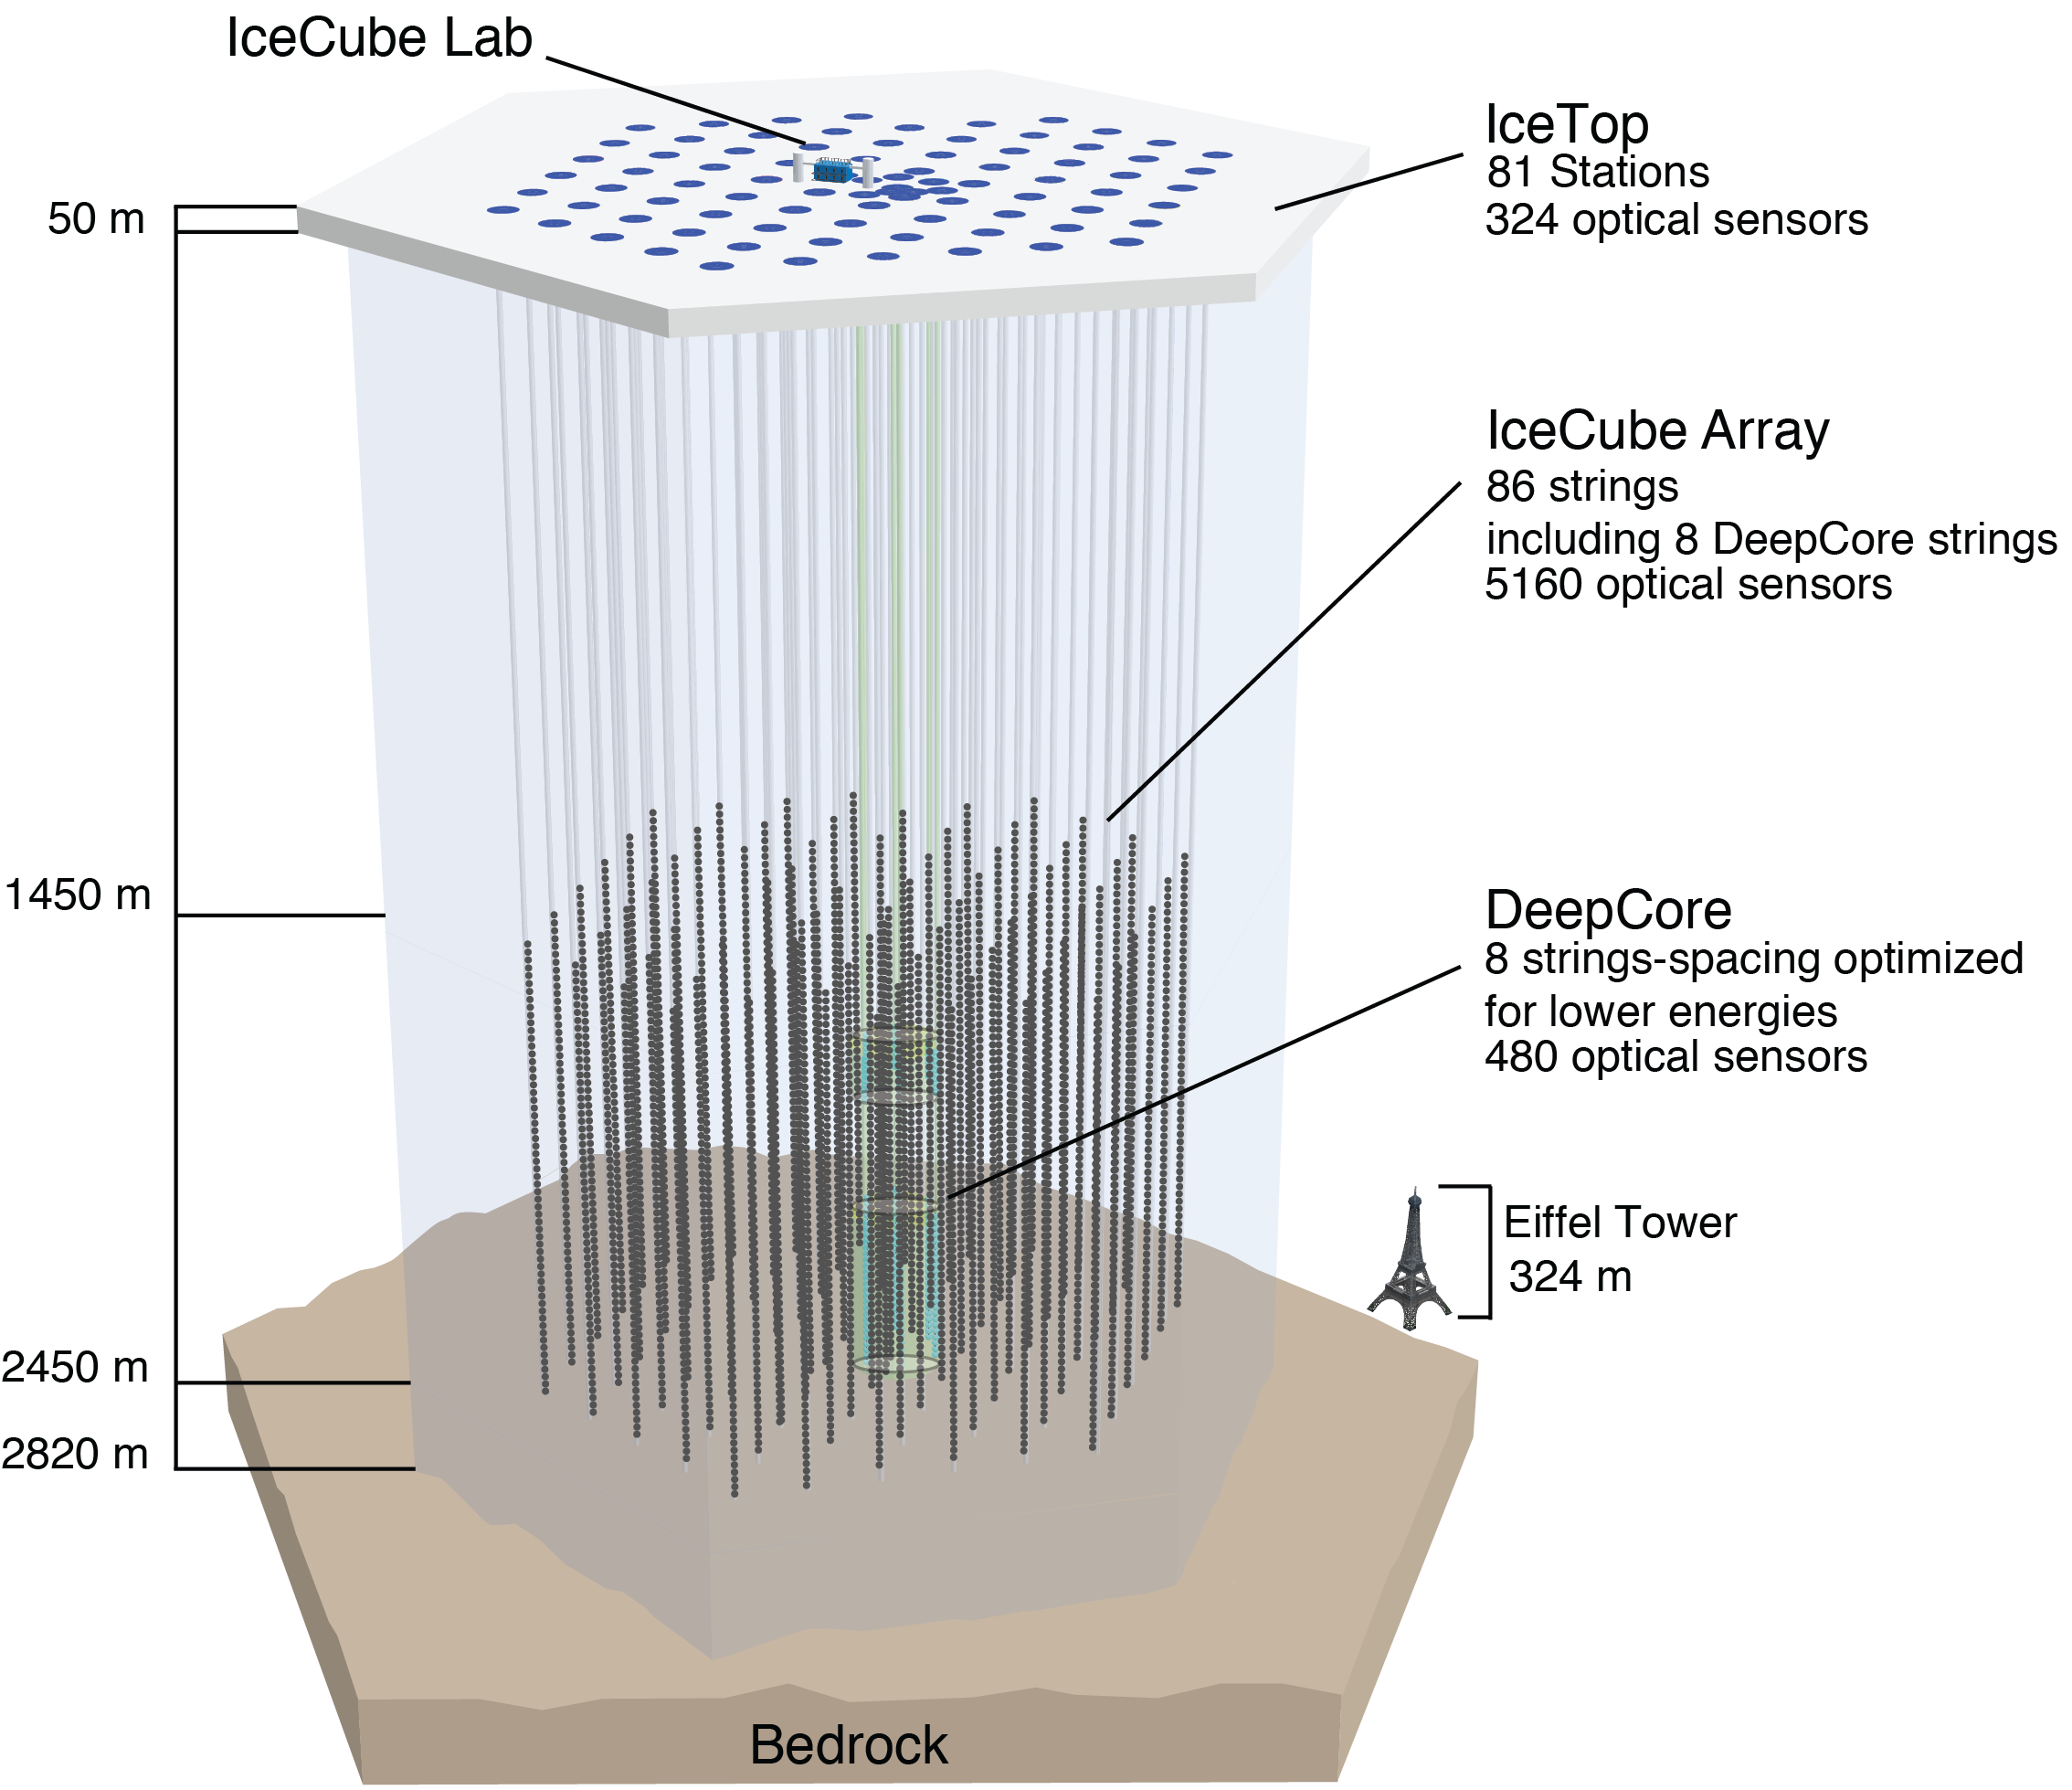
\includegraphics{./figures/nu_in_icecube/IceCubeArray_slim.png}
	\caption{A schematic overview of the IceCube detector and its components \cite{Aartsen_2017}}
    \labfig{ic_detector}
\end{figure}
    
\begin{marginfigure}
	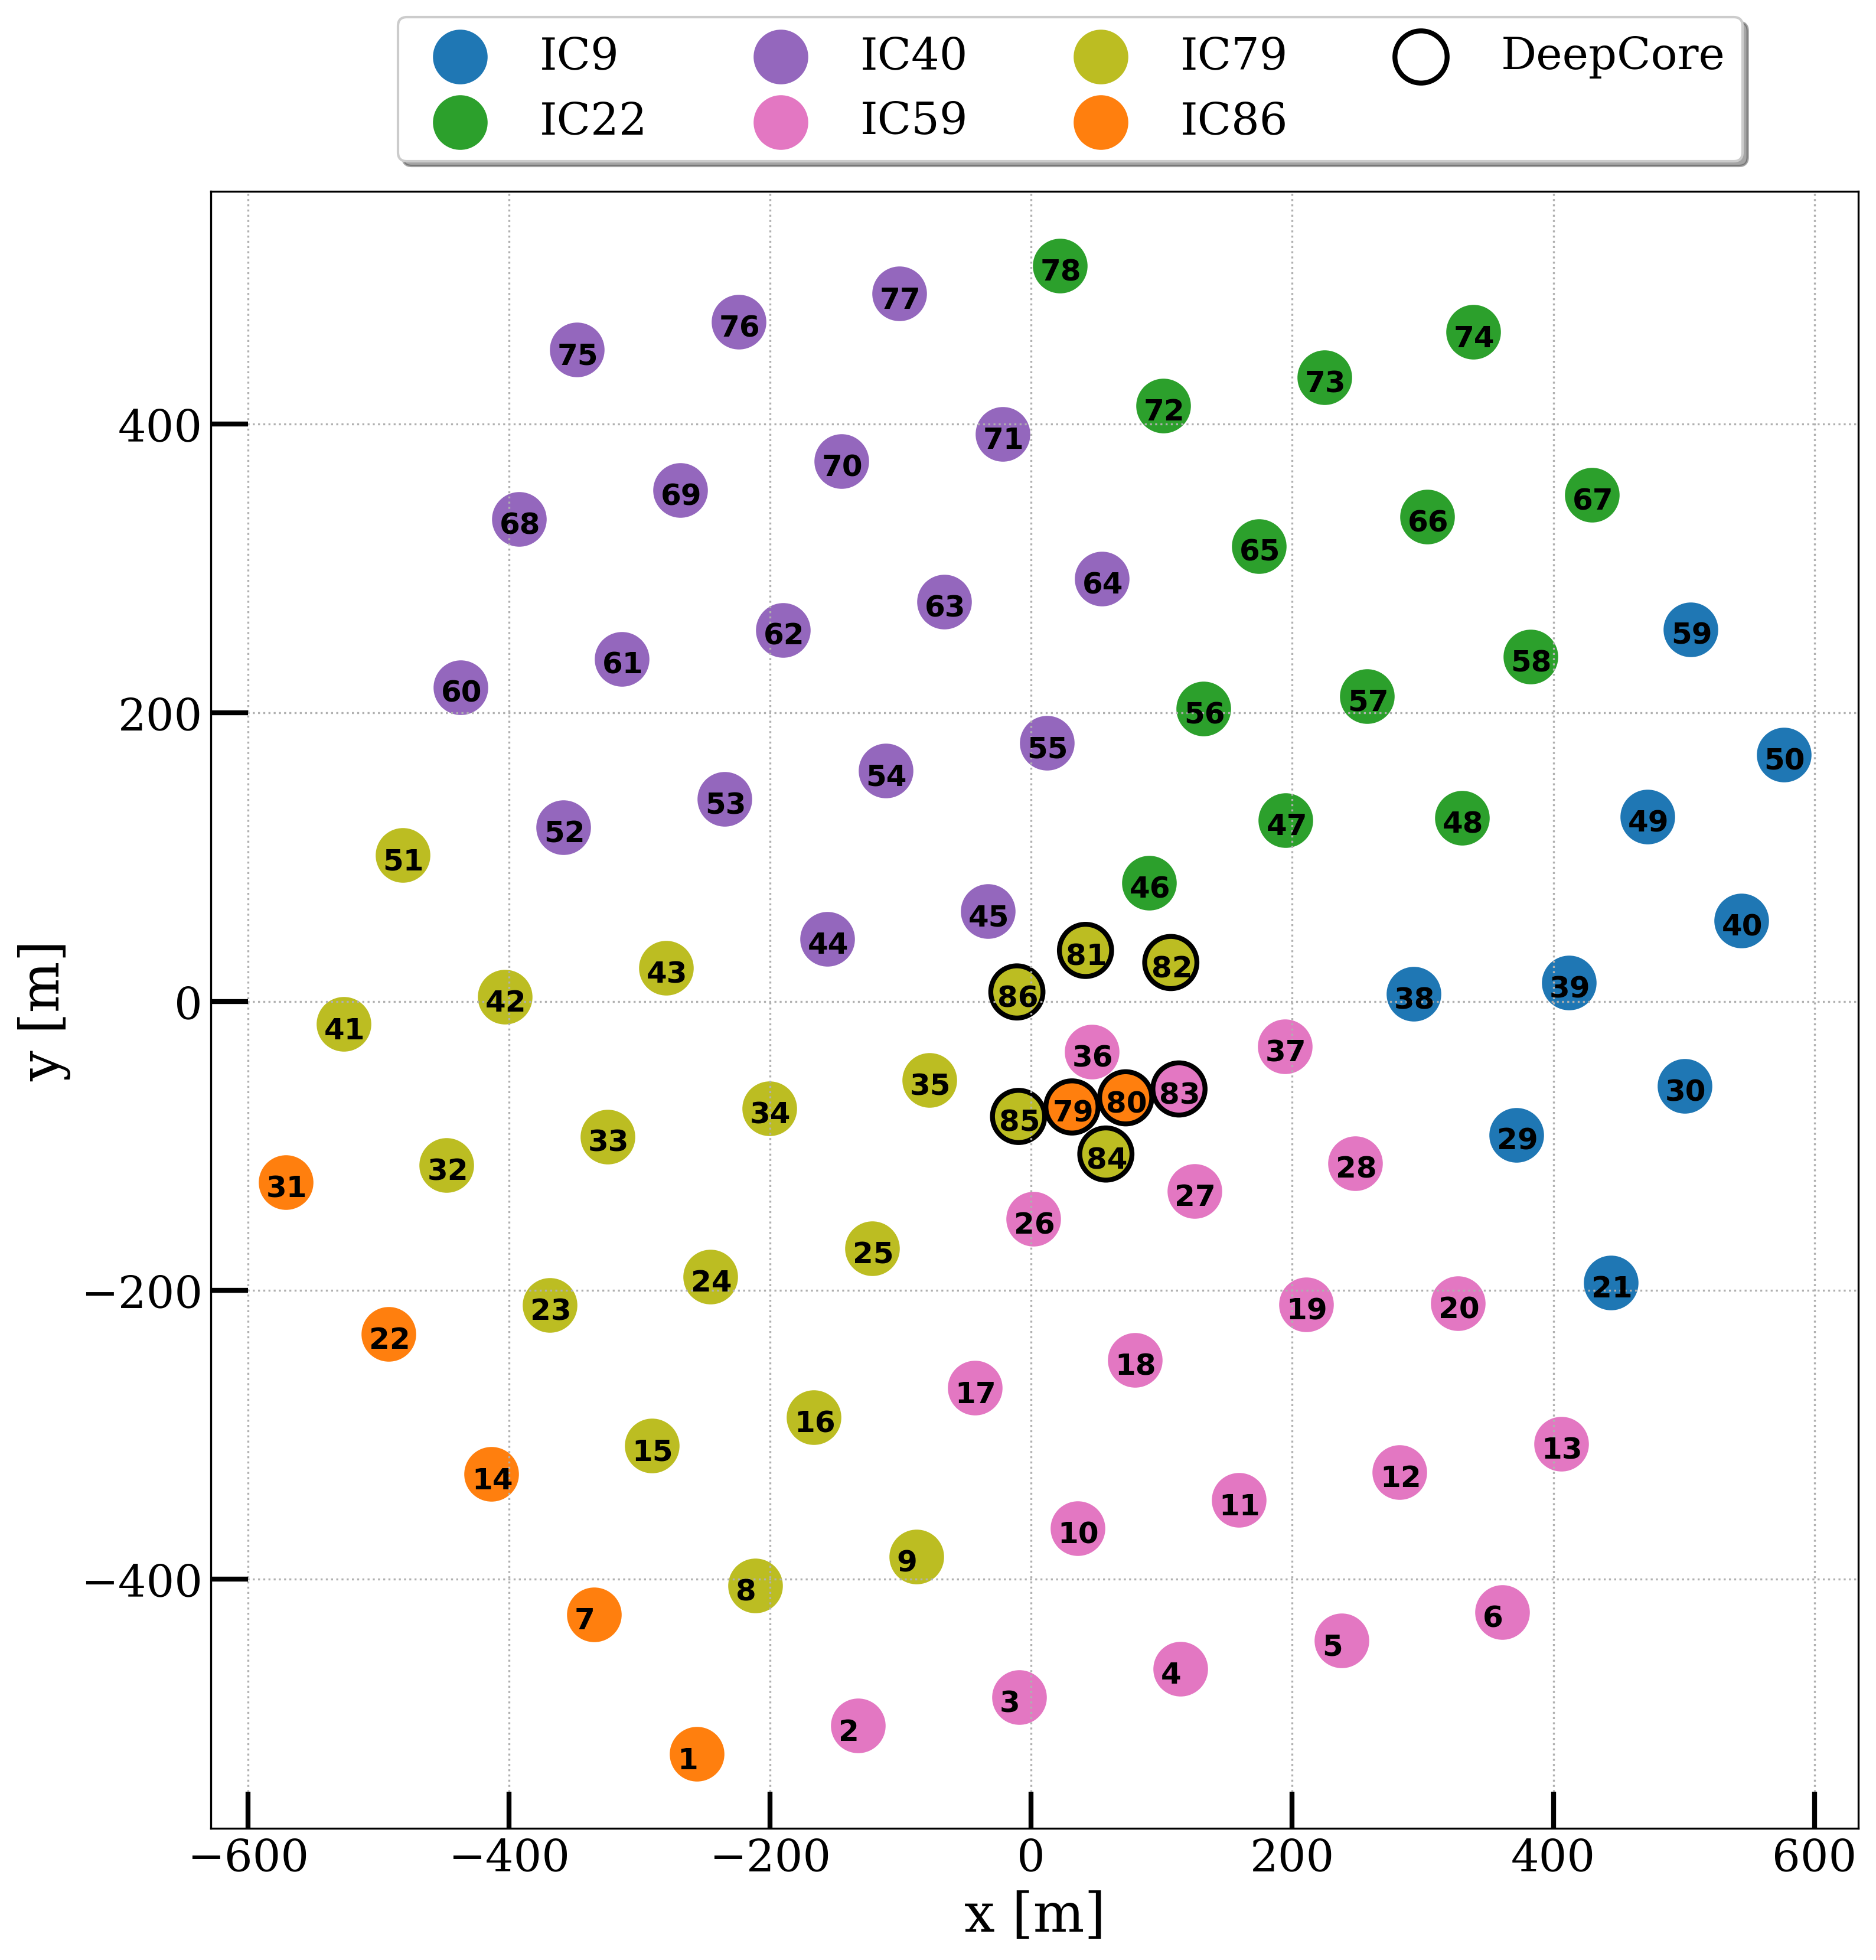
\includegraphics{./figures/nu_in_icecube/IC_Phase_Array.png}
	\caption{Top view of the location of each \emph{in-ice} strings of IceCube. Colour represents set of strings deployed in each seasons as described in \reftab{deployment_phases}. Note: IceTop Stations are not shown here.}
	\labfig{ic_phase_array}
\end{marginfigure}

\textbf{The IceCube Neutrino Observatory} is located at Amundsen-Scott South Pole Station at the geographic South Pole. It comprises a cubic kilometer of instrumented ice, equipped with 5,160 digital optical modules reffered as \emph{DOMs} from here-on (see \ref{sec:dom}), buried deep in the ice and 81 IceTop Stations on the surface of the ice, making itself the largest Neutrino Observatory in the world \sidecite{Aartsen_2017}. A schematic of the detector layout is shown in \reffig{ic_detector}. Four main components of the detector are \emph{in-ice array,DeepCore (inner extension of in-ice array),IceTop and IceCube Lab}. \par

\begin{description}
	\item[The Main \emph{in-ice} array] consists of 78 strings,\marginnote
    {\begin{kaobox}[title=\textbf{\emph{string} in IceCube}]
        An arrangement of DOMs attached on a twisted copper wire cable makes the so-called \emph{string} in IceCube.
    \end{kaobox}}
    each consisting of 60 DOMs, spaced vertically at a distance of 17 m between the depth of 1450 m to 2450 m under the ice sheet of Antarctica. Horizontal spacing between each of these strings is 125 m.  
	\item[\emph{DeepCore}] comprises inner 8 strings (see \reffig{ic_phase_array}) of the main\emph{in-ice} array, placed more closely together with horizontal string distance of 70 m and vertical DOM distance of 7 m \sidecite{deepcoredesign} between 1750 m to 2450 m depth. There's a region between depth of 1850 m to 2100 m, with no DOMs attached to the string as this region is the so-called \emph{dust layer} (see section \ref{sec:icemodel}), where optical scattering and absorprion is quite high and thus is not efficient to make reliable physics measurements. The Photomultipliers used in DOMs attached on these 7 strings also have higher Quantum Efficiency, which reduces the energy threshold to ~10 GeV. Although, IceCube's main goal is to detect astrophysical neutrinos, current topics of research spans much broader range (e.g fundamental properties of the neutrinos, such as oscillations \sidecite{Aartsen_2019_oscillations}, Physics beyond Standard Model searches such as Dark Matter \sidecite{Abbasi_2022} etc). 
	\item[\emph{IceTop}] is the surface detector array of the IceCube detector, primarily designed to detect Cosmic-ray airshowers and to be used as a veto layer for downgoing muons produced in these airshowers \sidecite{ABBASI2013188}. It consists of 81 \emph{stations} each having 2 tanks filled with clear ice (162 tanks in total). Each of these 162 tanks have 2 DOMs, similar to the ones deployed in \emph{in-ice} array, which makes it easier for both arrays to have a similar trigger and data acquistion system.
	\item[\emph{IceCube Lab}(ICL)] serves as the central operations' hub for the experiment, providing a crucial support for data acquisition and filtering. All the string cables connected to the aforementioned detcetor components are routed up to the ICL, from where triggered data is sent back to the northern hemispher via a satellite. Various other operations such as mainting the detector operations etc are also maintained from this building. 
	\end{description}

For the work presented in this thesis, neither \emph{deepcore} nor \emph{IceTop} data is used.
\begin{table}
    \caption{IceCube detector components deployed in each season (cumulative). Each configuration is represented as \emph{ICXX} where \emph{IC} stands for IceCube and \emph{XX} stands for number of total \emph{in-ice} strings at the end of that season}
    \labtab{deployment_phases}
    \begin{tabular}{cccc}
        \hline
        \hline
        Season & Configuration & Strings & IceTop Stations\\
        \hline
        2004-05 & IC1 & 1 & 4\\ 
        2005-06 & IC9 & 9 & 16\\ 
        2006-07 & IC22 & 22 & 26\\ 
        2007-08 & IC40 & 40 & 40\\ 
        2008-09 & IC59 & 59 & 59\\ 
        2009-10 & IC79 & 79 & 73\\ 
        2010-11 & IC86 & 86 & 81\\  
        \hline
        \hline
    \end{tabular}
    \end{table}


\marginnote{
    \begin{kaobox}[title=IceCube coordinates system]
        The IceCube coordinate system's origin is at 46500'E, 52200'N, 883.9 m elevation, which is quite close to centre of the \emph{in-ice} array. The y-axis points Grid North (toward Greenwich, UK), the x-axis points Grid East (90 degrees clockwise from North), and the z-axis points "up", forming a right-handed coordinate system.
     \end{kaobox}
    } 
The construction of the detector started taking place in 2005 and lasted for 7 Antarctic summer seasons till 2011 December. In each season, parts of the current day Hexagonal detector were deployed, as shown in \reffig{ic_phase_array} and numbers detailed in \reftab{deployment_phases}. A hot water drill was used to unfreeze the ice upto 2.5 km depth and 60 cm diameter into which these strings were then deployed (see \reffig{DOM_assembly}). The geometry of the detcetor, i.e The \emph{xy}-coordinates of the string were calculated from the drill tower position, surveyed during the deployment. Assuming the string was vertical, these coordinates were applied at all depths, with deviations of less than 1 m (later validated using the flasher data, see \ref{sec:DAQ}). Depths of the lowest DOM were determined from pressure readings, corrected for water compressibility and ambient air pressure, with vertical DOM spacings measured via laser ranger. All depths were converted to z-coordinates in the IceCube coordinate system \todo{Maybe draw a small schematic of coordinate system here next to the side note?}.\par  


\subsection{The Digital Optical Module (DOM)}
\label{sec:dom}
\textbf{The Digital Optical Module} (DOM) is a crucial component of the IceCube Neutrino Observatory, functioning as the heart of the detector. Each DOM is responsible for collecting the faint light signals produced by neutrino interactions in the Antarctic ice, amplifying these signals, and transmitting the data to the IceCube Lab \cite{Aartsen_2017}. From there, the data is relayed to the Northern Hemisphere via a satellite for further analysis. 

Inside each DOM, a 10-inch Photo Multiplier Tube (PMT) is positioned at the bottom, accompanied by essential circuitry for power conversion, data acquisition, calibration, control, and data transfer. Individual components of a DOM are as shown in \reffig{DOM_schematic}, functions of each of which is explained briefly below.

\begin{description}

    \item[Glass Vessel Properties :] The glass vessel of the DOM is engineered to withstand the extreme pressures found in the deep Antarctic ice. This includes the constant long-term pressure of about 250 bar and the temporary pressure spikes of up to 690 bar experienced during the refreezing process after deployment using a hot water drill. The vessel is composed of two 0.5-inch thick hollow glass hemispheres, which are joined together with optical glue. This design not only provides a robust and hermetic seal to protect the internal electronics but also maintains the optical clarity necessary for the PMT to function effectively. The glass material is chosen for its strength, transparency, and resistance to the harsh conditions in the ice.

    \begin{marginfigure}
        % \vspace*{4.5cm}
        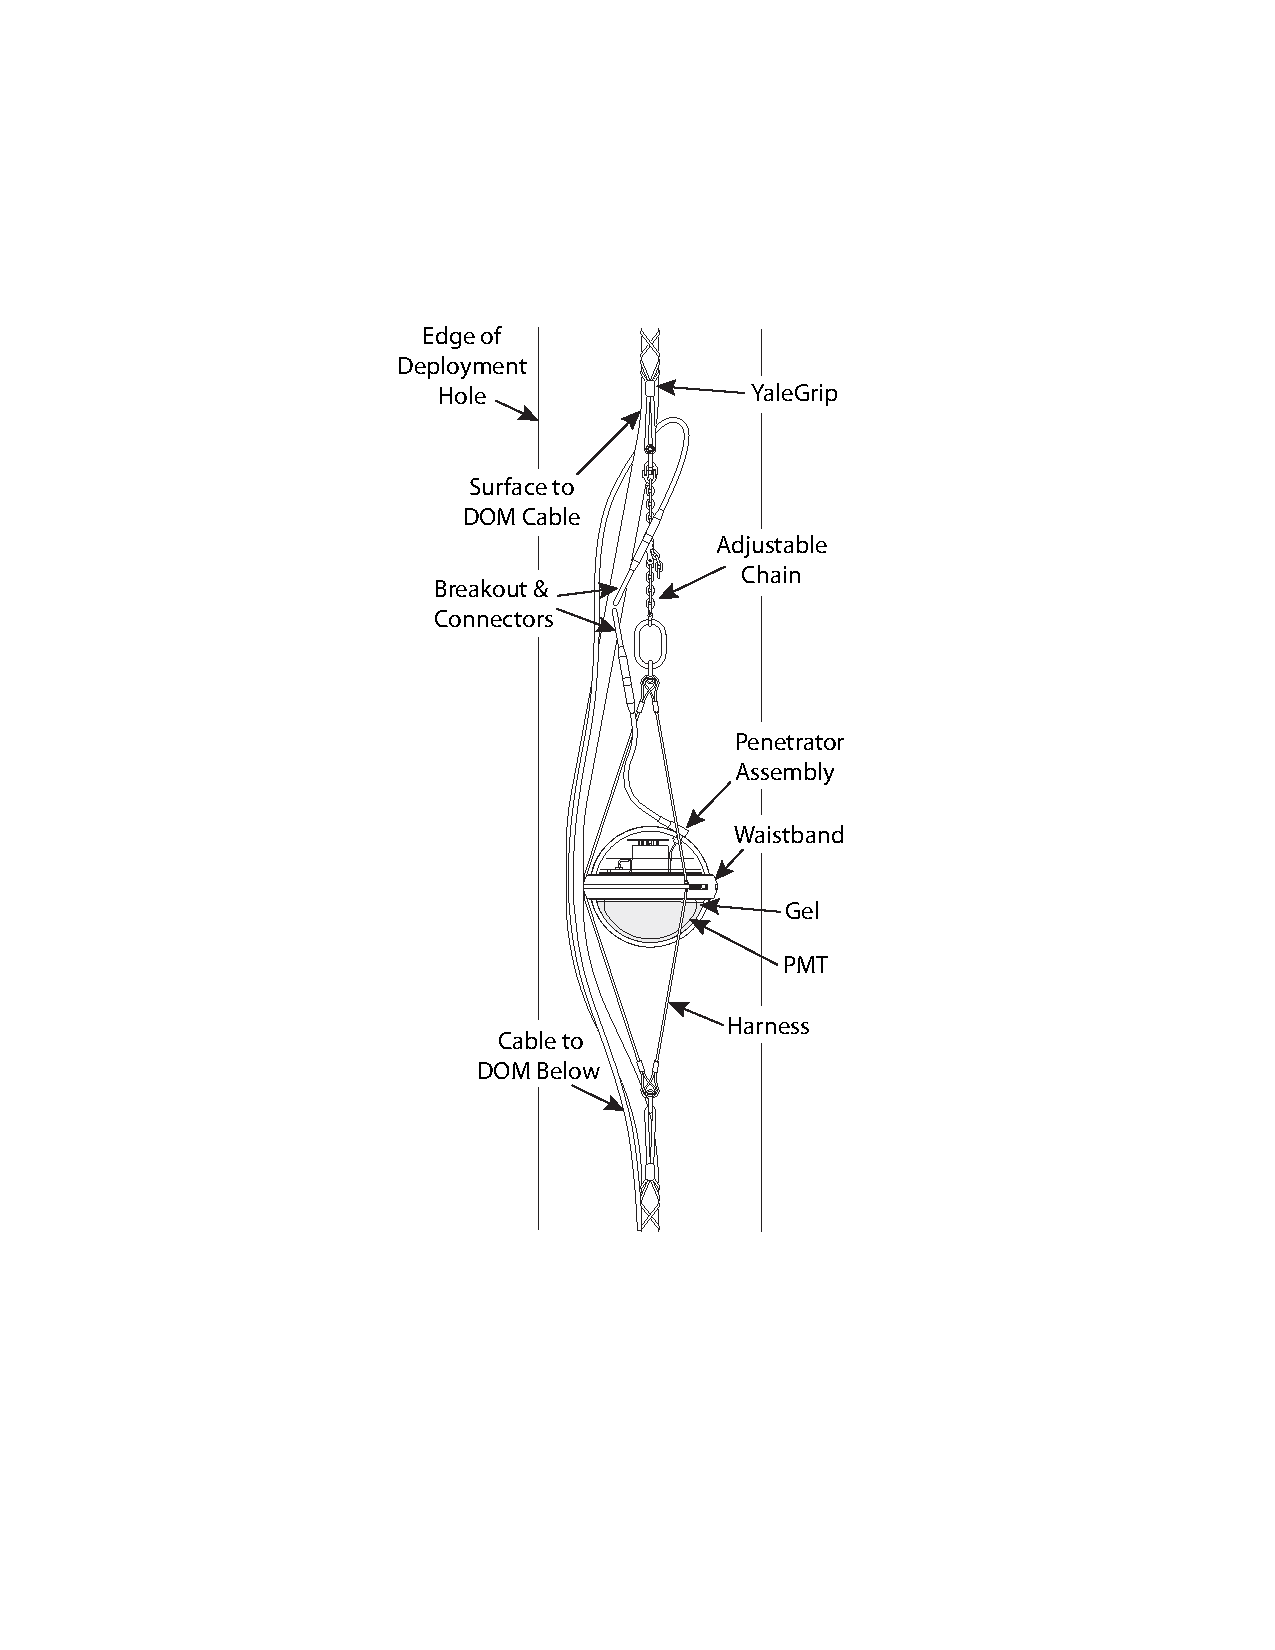
\includegraphics{./figures/nu_in_icecube/domfig2a-CableAssembly.pdf}
        \caption{A schematic of DOM CableAssembly being deployed in a water hole, created by hot water drill \cite{Aartsen_2017}.}
        \labfig{DOM_assembly}
    \end{marginfigure}
    
    \begin{marginfigure}
        % \vspace*{4.5cm}
        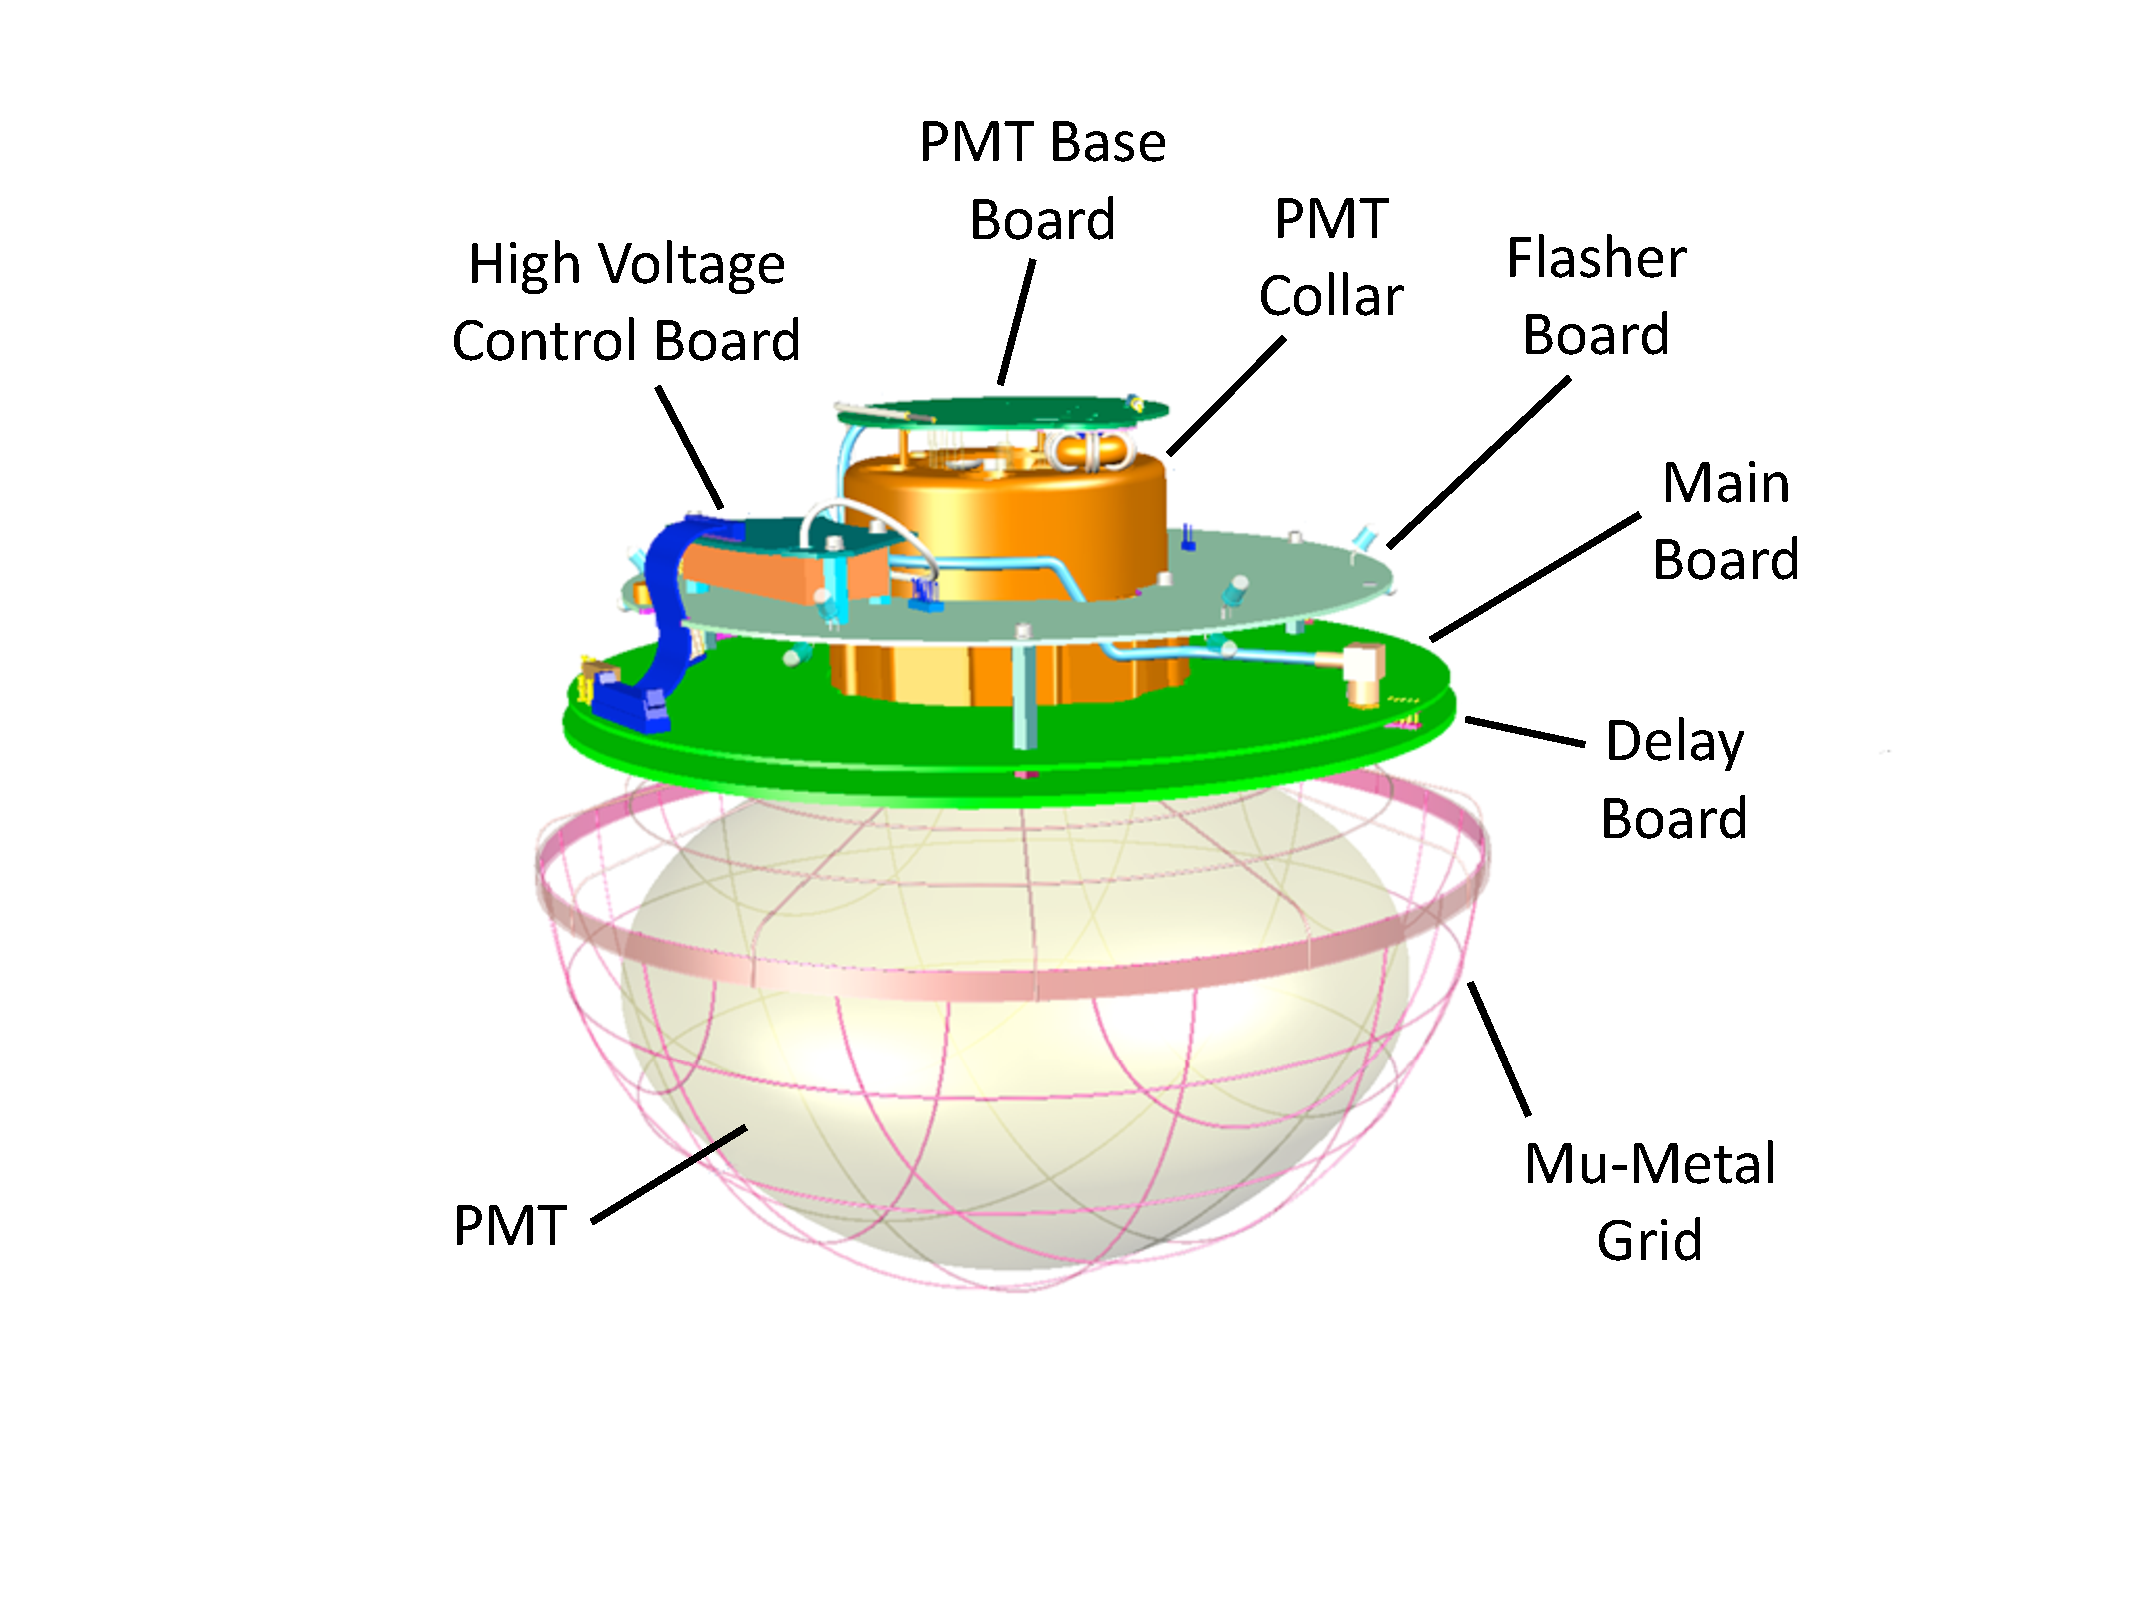
\includegraphics{./figures/nu_in_icecube/domfig1a-DOM3DModel.pdf}
        \caption{A schematic of the DOM, showing its main components \cite{Aartsen_2017}.}
        \labfig{DOM_schematic}
    \end{marginfigure}

    \item[PMT :] The PMT within the DOM is a 10-inch diameter tube that utilizes a box-and-line dynode chain with 10 stages to amplify the faint light signals detected in the ice. The PMTs used in standard in-ice DOMs have a quantum efficiency peaking at 25\% whereas, DeepCore DOMs, designed to detect lower energy neutrinos, feature PMTs with a higher peak quantum efficiency of 34\% near the 390 nm wavelength. These PMTs are operated at a gain of $10^7$.

    \item[Gel :] A high strength, silicon gel is used between the photocathode area and the glass vessel to provide optical coupling and strong mechanical support to the DOM system. This gel has a high optical clarity, with 97\% transmission at 400 nm. It shows no signs of deterioration even after a decade, ensuring reliable performance.

    \item[Magnetic Shield :] The ambient magnetic field at the South Pole, measuring around 550 milligauss (mG), angled 17 degrees from vertical, can significantly affect the performance of the PMT. This includes reducing collection efficiency by 5-10\% and causing gain variations of up to 20\%, depending on the PMT's azimuthal orientation. To mitigate these effects, a mu-metal cage is installed around the PMT bulb, extending up to its neck. This cage is constructed from a mesh of 1 mm diameter wires with a spacing of 66 mm. Although this mesh blocks about 4\% of the incident light, it substantially reduces the adverse impacts of the magnetic field, ensuring more consistent and reliable performance of the PMT.

    \item[PMT Base and High Voltage Boards :] The high voltage board includes a Digital to Analog Converter (DAC) and an Analog to Digital Converter (ADC) for precise control and monitoring of the voltages supplied to the PMT. The high voltage generator on this board provides the necessary power, which is then regulated and distributed by the voltage divider circuits on the PMT base board. These circuits are specifically designed for low power consumption, ensuring efficient and stable operation of the PMT.
    
    \item[Main Board :] The main board serves as the central processing unit (CPU) of the DOM, managing and coordinating all other electronic components. It digitizes the waveforms detected by the PMT, providing a digital representation of the light signals for further analysis. The main board also temporarily stores data, calibrates the internal clock, and exchanges local coincidence information with neighboring DOMs (see \ref{sec:DAQ}). It communicates directly with the Data Acquisition (DAQ) system, ensuring the seamless transfer of data to the IceCube Lab. Additionally, the main board hosts an adjustable low-intensity optical source, which is used to calibrate the PMT's gain and timing, ensuring consistent and accurate performance.
    
    \item[Flasher Board :] Flasher board contains 12 LEDs each having specified output wavelength of $405\pm5 \mathrm{nm}$,
    %  \marginnote{
    %     \begin{kaobox}[title="color DOMs" or CDOMs]
    %         16 of the 5160 \emph{in-ice} DOMs have multi-wavelength LEDs on their Flasher boards. 8 of these DOMs are on string 79 (quite at the centre of the detector, one of the DeepCore strings) and the other 8 on string 14 on the edge of the detector. 
    %     \end{kaobox}}
        which generates lights \emph{in situ} to make various caliberation related measurements. In addition, this board can verify timing responses (useful for many, including analysis presented in this thesis, reconstruction processes). Additionaly, to measure \emph{the optical properties} of the South Pole Ice (see section \ref{sec:icemodel}) and locations of the DOMs in ice.
    
\end{description}

\subsection{Trigger and Data Acquisition}
\label{sec:DAQ}
Ever Since the initial deployment of the first string, the detector has been consistently gathering data, maintaining an average uptime of nearly 99\% \sidecite{Abbasi_2009}. \emph{The photocathode} of the PMT of a DOM, \emph{captures} a photon which then generates \emph{photoelectrons} which are accelerated through the series of 10 dynodes to generate measurable \emph{photocurrent}. This current is integrated over a time to obtain collected charge in units of \emph{photoelectrons or PEs}, through which \emph{photovoltage} is produced at the mainboard, over time, known as \emph{waveform}. These waveforms are then digitized to acquire and relay the data to the Northern Hemisphere.

Depending on how many photons hit the PMT, these waveforms can have different amplitudes ranging from 1mV upto the linearity limit of the PMT (~2 V) in time range of 12-1500 ns. The In Order to access this rather broad dynamic range, the digitiser used, Analog Transient Waveform Digitiser (ATWD) have three channels to amplify the waveform by factor of 0.25, 2 and 16. Moreover, 2 sets of ATWD are used that can operate alternatively in order to reduce the deadtime. ATWD can digitize voltage withinn duration of 427 ns, a window sufficient to reconstruct light produced within 10s of m around a given DOM. Naturally, some photons produced in energetic interactions may travel larger distances, producing faint but detectable waveforms. To amplify and digitize these waveforms, a fast Analog to Digital Converter (fADC) is also used, together ATWD+fADC is reffered as a \emph{DOMLaunch}.

The aforementioned digitization only happens if the voltage threshold of the onboard discriminator is met, which is kept at voltage equivalent to a PE of 0.25, or in other words, a DOM is \emph{hit}. If at least two neighbouring DOMs, on the same string produces individual \emph{hits} within 1 $\mu\mathrm{s}$ called \emph{Hard Local Coincidence(HLC)}, the full \emph{DOMLaunch} is transmitted to the surface. Otherwise, only the timestamp and minimal amplitude/charge information is sent known as \emph{Soft Local Coincidence(SLC)}. The HLC condition helps reduce false triggers from PMT dark noise, which is independent across DOMs. \emph{The Data Acquisition System (DAQ)} processes further uses these HLC hits to look for temporal coincidences. Most commonly used trigger in IceCube is the so-called \emph{The Single Multiplicity Trigger (SMT-8)}, that requires eight or more HLC hits within 5 $\mu\mathrm{s}$ timewindow. If and when SMT8 trigger conditions are met, all launches (HLC and SLC) are combined into what is called an \emph{event}. 

Various algorithms are used to make an estimate of event properties such as direction, deposited energy, morphology etc. The South Pole has limited computational resources, so only simple first guess algorithms can be used there called \emph{online filters}. Processed data is transmitted to the Northern Hemisphere. After this, more sophisticated reconstruction algorithms are applied to reduce and tailor the data as per Physics analysis goal. \todo{cite simulation/reco chapter here}


\section{Optical Properties of the South Pole ice}
\label{sec:icemodel}
\begin{marginfigure}
	\centering 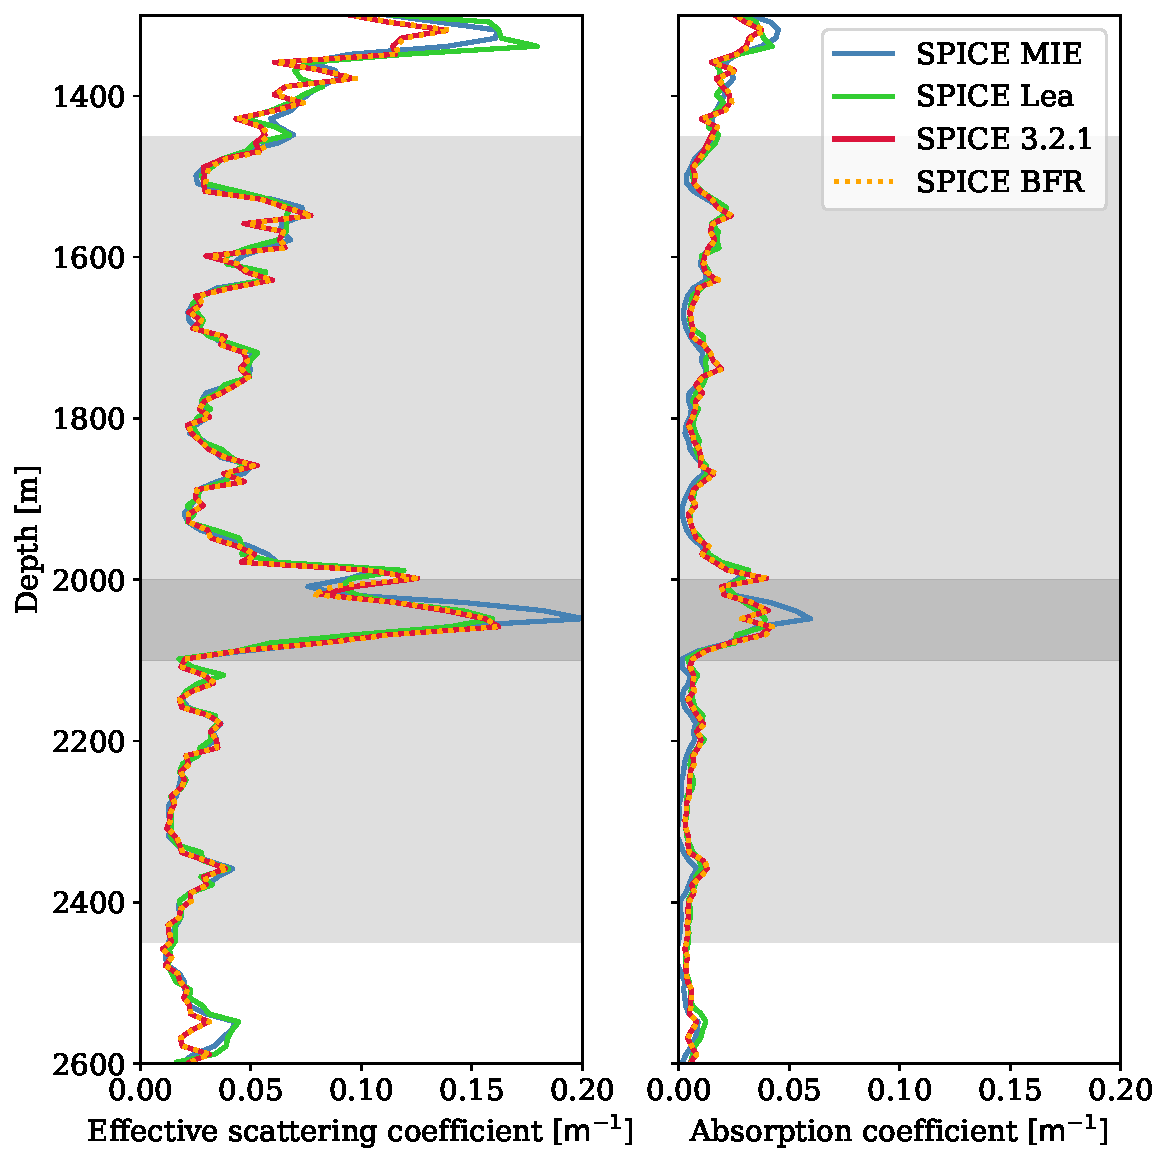
\includegraphics{./figures/nu_in_icecube/abs_scat.pdf}
	\caption{Values of effective scattering (left) and absorption (right) coefficents of 400nm photons in South Pole Ice as a function of depth, for four icemodels described in the text. Light grey area shows in-ice array and dark grey region shows the high absorption and scattering region called \emph{the dust layer}.}
    \labfig{abs_scat}
\end{marginfigure}
The ice at the South Pole is a crucial part of the IceCube detector. It acts as both the detection target and the medium through which light propagates. Unlike the DOM hardware, which has been extensively studied in the laboratory, the glacial ice can only be measured in its actual environment, making it more challenging to describe. Understanding and calibrating this medium well is essential for accurate physics measurements as photons produced from particle interactions can get absorbed or scattered from their path, making the inference of the particle interaction points challanging.

In context of Neutrino Detection, The ice at the deep South Pole was initially measured using pulsed in situ light sources (LEDs) at different wavelengths, embedded in the AMANDA array below ~1000 m depth\sidecite{optical_properties_amanda}. Later, during the construction of IceCube, direct measurements of dust concentration in the glacial ice were obtained using a dust logger deployed into some drill holes \sidecite{dust_logger}. Additionally, the LEDs on the Flasher Board of DOMs are still actively used to calibrate the detector and understand the ice properties \sidecite{spicemie}. 

\textbf{The scattering length ($\mathrm{l}_s$)} is the average distance a photon will travel before scattering off of its orignal directory. In practice, only the effective scattering length ($\mathrm{l}_\mathrm{eff}$ = $\frac{\mathrm{l}_s}{1 - \langle\cos\theta\rangle}$) can be measured, where $\langle\cos\theta\rangle$ is the average deflection angle at each scatter. \textbf{The absorption length ($\mathrm{l}_a$)} is the distance after which a photon's survival probability decreases to 1/e, indicating how far the information from an event can travel. In the case of absorption, the photon is lost, while for scattering, its direction changes, affecting both the energy and direction reconstruction of the event. Scattering and absorption parameters in \emph{ice models} are averaged over 10-meter-thick layers of ice and are calculated for a wavelength of 400 nm \cite{spicemie}. Light scattering below a depth of about $\sim$1300 m is mainly due to residual air bubbles. As depth increases, dust becomes the main source of scattering, with concentration varying due to climate and volcanic activity. At around 2000 meters, scattering and absorption significantly increase due to high dust concentration, possibly from a major volcanic eruption in the past, known in IceCube as \textbf{the dust layer} \sidecite{dustlayer} (see \reffig{abs_scat}). This layer is either ommitted or treated more carefully in most analyses as information carried by photons coming and going throught this layer is difficult to traceback due to higher scattering coeeficient.
\begin{figure}
	\centering 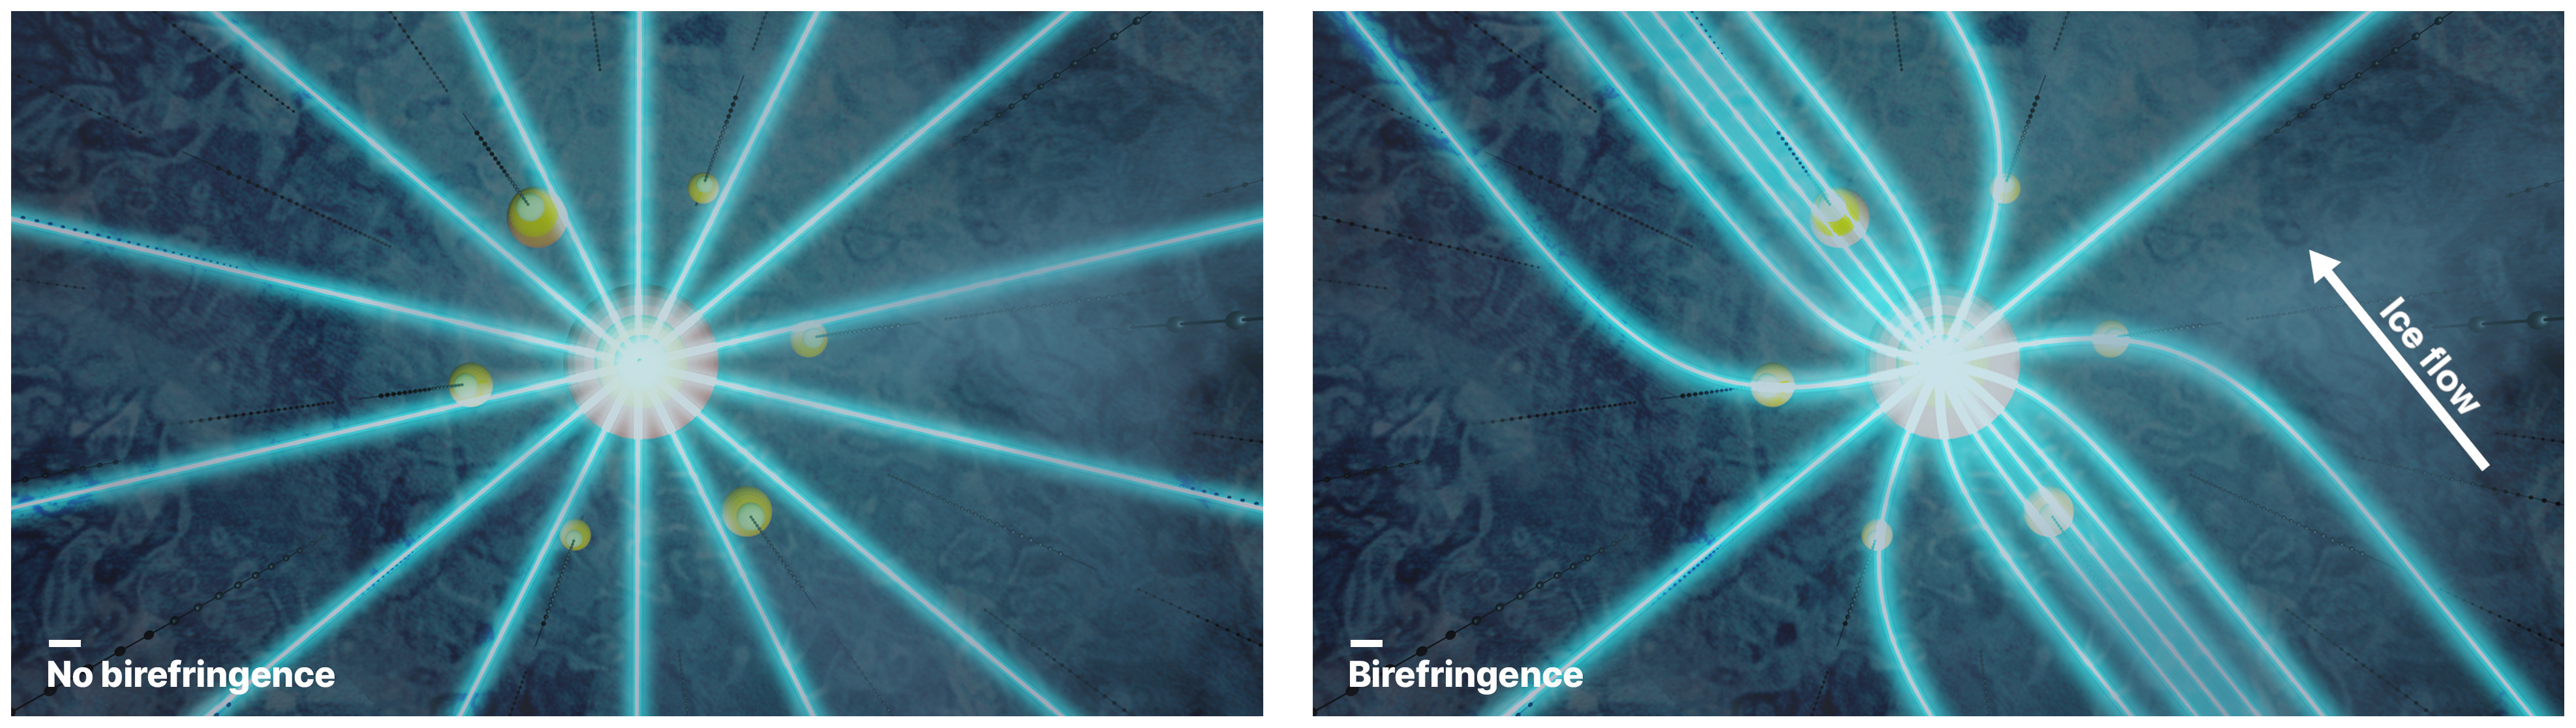
\includegraphics{./figures/nu_in_icecube/bfr_illustration.png}
	\caption{The visualisation of deflection due to birefringence. Without it (left panel), light streams out radially from an isotropic source. With this effect however (right panel), rays get deflected towards the flow axis, appearing as though photons are scattered "more" along this axis. The IceCube array around the light source can be seen as well. (Figure taken from \cite{BFR_paper})}
    \labfig{bfr_effect}
\end{figure}

The data from the dust logger also revealed that the ice layers are not perfectly horizontal; they are tilted due to the uneven surface of the bedrock \cite{dust_logger}, the so-called \textbf{ice tilt}. Initially, the effect was symmetrically parameterized along an axis (reffered to as \emph{the tilt axis}) that is approximately perpendicular to the glacial flow and also dependent on depth (same as the layers used to characterise absorption and scatetring lengths described before)\cite{spicemie}. As a result, the scattering and absorption coefficients became dependent on the full three-dimensional position in the ice rather than just the depth. A recently developed fully volumetric tilt model now includes a newly discovered tilt component along the flow \sidecite{tilt_icrc}.


Another unique property that the South Pole ice exhibits is optical \textbf{anisotropy}, a phenomenon affecting photon propagation depending on their direction relative to the "axis of anisotropy," which coincides within $\sim 1^\circ$ with the direction of the ice flow \cite{spicemie}. This effect was initially implemented as a modification to the scattering function, the only remaining Mie scattering parameter \sidecite{miescattering}, thereby changing the scattering length \sidecite{bfr_icrc2013,marcel_thesis}.  However, recent detailed studies suggest that this behavior results from diffusion within the polycrystalline ice microstructure, a previously unknown optical effect, now known as Birefringence \sidecite{bfr_icrc2019,BFR_paper}. This effect causes the ice crystals to slowly but continuously deflect towards the normal vector of the girdle plane of the crystal orientation fabric (the ice flow axis), as can be seen in \reffig{bfr_effect}.



In the context of the IceCube Detector, South Pole ice can be divided into two types: bulk ice and hole ice. Bulk ice is the undisturbed part of the ice, consisting of sheets that have formed over hundreds of thousands of years, properties of which are described above. \textbf{Hole ice}, on the other hand, is the refrozen column of ice that was melted during the deployment of the DOMs \sidecite{holeice_dima_icrc21}. This effect generally affects the forward acceptance of the IceCube DOMs. If not taken care of, it can lead to errors in directional information, therby affecting measurements involving zenith angle reconstructions of the incoming neutrino. Over the years, many efforts have been made to understand various optical properties of the South Pole ice, by fitting the LED data in terms of absorption and scattering lengths of a cherenkov photon in ice, the so-called \textbf{\emph{South Pole ICE model (SPICE model)}}. These icemodels are used in both simulation and reconstruction of the events, where particles produced in neutrino interactions are propagated (see \ref{sec:particle_propgation}) based scattering and absorption lengths described by the model. While the base model for the scattering of the photons in-ice is Mie Scattering theory \cite{miescattering} (SPICE MIE), with more dust loggers data, evolved more complex models to include, aniostropy (SPICELea), addition of tilt (SPICELea, SPICE 3.2.1), birefringence to explain anisotropy (SPICEBfr) and the latest, SPICE FTP, which includes a 2D tilt corretion in addition to birefringence. \reffig{abs_scat} shows absorption and scattering coefficients for different ice models at various depths in the detector. The corresponding scattering and absorption lengths are simply the inverse of the coefficients. It can be seen that the ice below the depth of $\sim$ 1400 m is so clear that light can travel for hundreds of meters before being absorbed. However, the light diffuses quickly, making a point-like source appear nearly isotropic at a distance of around 100 m. Effect of different icemodel corrections (specifically that of anisotropy related corrections) becomes quite relevant to reconstruct tau-neutrino events in IceCube (see Section~\ref{sec:icemodel_checks}), which is heart of the analysis presented in this thesis.


\section{Detection of Neutrinos in IceCube}
\label{sec:nu_detcetion_ic}
As described in \ref{sec:DIS}, regardless of the type of neutrino interaction (NC or CC), a variety of secondary particles are generated. In the case of a CC interaction, an accompanying charged lepton absorbs some energy, which can then undergo further decay or interact within the ice volume, leading to the production of more particles. Moreover, secondary particles, regardless of the interaction type, may also include hadrons, which are not always charged. This can, in turn, reduce the amount of \emph{visible} light in the detector. In this section, propagation of these leptons and hadrons in ice shall be explained in brief, followed by Cherenkov effect, a phenomenon by which IceCube DOMs observes these photons from the neutrino interactions. Lastly, various morphologies of these interactions will be discussed in the context of IceCube and similar detectors.

\subsection{Particle propgation in-ice}
\label{sec:particle_propgation}
When a charged particle moves through a medium like ice, it loses energy due to interactions with the medium's particles. This energy loss is characterized by the quantity $ \frac{dE}{dx} $, where $ dE $ represents the energy lost and $ dx $ the area of the medium traversed, typically measured in $\text{g/cm}^2$. Four primary processes contribute to the energy loss profile of a particle in such a medium: continuous ionization losses and radiative losses due to bremsstrahlung, pair production, and photonuclear interactions. \emph{Ionization} occurs when the particle collides with shell electrons of the atoms in the medium, causing a continuous energy loss that scales logarithmically with the particle's energy \sidecite{PDG_2024}. Additionally, if the particle is unstable, it may decay. In the context of IceCube, secondary leptons travel at nearly the speed of light, simplifying $ \beta $ to approximately 1. Thus, the decay length can be rewritten as $ \lambda_{\text{dec}} = \frac{E\tau}{mc} $, where $ E $ is the lepton's energy and $ m $ its mass. The decay length indicates the distance at which the lepton's survival probability drops to $ \frac{1}{e} \approx 36.8\% $, following the exponential decay law $ p(L) = \exp(-L/\lambda_{\text{dec}}) $.

Radiative losses, such as \emph{bremsstrahlung}, occur when the charged particle is deflected through Coulomb scattering off a target atom, while \emph{pair production} involves the creation of an electron-positron pair by an emitted photon. \emph{Photonuclear interactions} occur when a photon emitted by the particle disintegrates an atomic nucleus. These radiative losses are stochastic and scale roughly linearly with the particle's energy, with the radiation length $ X_0 $ defining the distance over which the particle’s energy decreases to $ \frac{1}{e} $ of its initial value \cite{PDG_2024}. The overall energy loss can be expressed as, 
\begin{equation}\label{eq:1}
    -\frac{dE}{dx} = a(E) + b(E)E 
\end{equation}
where $a(E)$ represents ionization losses and $b(E)$ encompasses all radiative losses.

\subsubsection{Leptons}
\label{sec:leptons_inice}
To determine a neutrino's flavor, it's important to understand the energy losses of the charged lepton created in a CC-interaction. The radiation length varies depending on the lepton's mass, influencing emitted radiation and aiding in lepton identification. For leptons with $ \beta\gamma \gg 1 $, this ionization loss can be approximated as constant, with a value of $\langle \frac{dE}{dx} \rangle_{\text{ion}} \approx 2 \, \text{MeV/(g/cm}^2)$ \sidecite{Perkins}. In ice, this corresponds to a continuous energy loss of approximately 180 MeV per meter. However, at energies exceeding \emph{critical energy ($\mathrm{E}_\mathrm{c}$)}, radiative losses become dominant, and ionization losses become negligible, as shown in the \reffig{e_loss} \sidecite{MMC_paper}. 

For \textbf{electrons}, we mainly consider radiative losses (mainly bremsstrahlung see \reffig{e_loss}) as they are stable and do not decay. Photons from bremsstrahlung then create additional $e^+e^-$ pairs which can create more photons and so on, resulting in a cascade of particles until the energies of electrons and positrons fall below the critical level. This behavior can be described by a gamma distribution, regardless of what the initiating particle is ($e^+ \, e^- \mathrm{or} \, \gamma$) \cite{PDG_2024}. The rate of energy loss over distance can be calculated using the equation:

\begin{equation}\label{eq:2}
    \frac{dE}{dt} = E_0 b \left( \frac{(bt)^{a-1} e^{-bt}}{\Gamma(a)} \right)
\end{equation}

\begin{figure}
	\centering 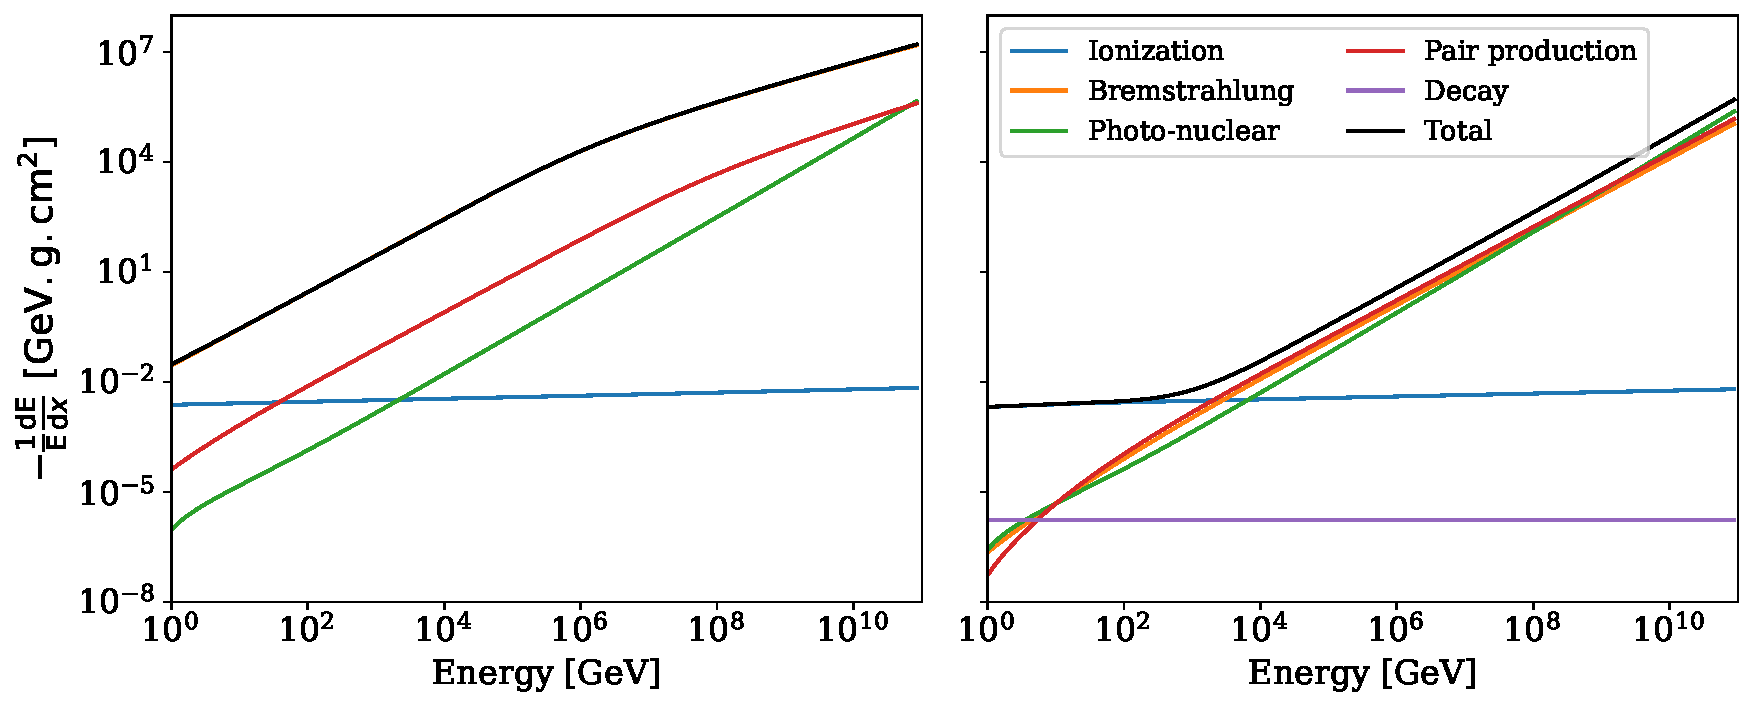
\includegraphics{./figures/nu_in_icecube/energylosses.pdf}
	\caption{The average energy loss rate per energy, for electrons (left) and muons (right) in
    ice showing the contributions from ionization, bremsstrahlung, photonuclear interactions, and pair production. Note that decay is only shown for Muons as electrons are stable particles that do not decay. Figure reproduced from \cite{MMC_paper}}
    \labfig{e_loss}
\end{figure}


Where $t$ represents the distance along the cascade in units of radiation length, and $E_0$ is the initial energy of the injected particle and $a$ and $b$ are dimensionless shower parameters. For an electromagnetic cascade induced by an electron, the parameters are $a = 2.02 + 0.63 \log(E_0/\text{GeV})$ and $b = 0.63$ (determined using \texttt{GEANT4} simulations \sidecite{shower_profile} ). The distance to the shower maximum, $t_{\text{max}}$, which is given as $t_{\text{max}}=\frac{a-1}{b}$ characterizes the size of electromagnetic cascades, indicating that they grow logarithmically in size with energy and have a characteristic size of several meters. This justifies the common approximation that light is emitted from a single point, a useful assumption for simulation and event reconstruction purposes (see Section~\ref{sec:reco} of \refch{nu_samples} for details).

At very high energies ($>10$ PeV), \emph{the Landau-Pomeranchuk-Migdal (LPM) effect} becomes significant, causing suppression of bremsstrahlung and pair production cross sections \sidecite{LPM1,LPM2,LPM3}. This suppression occurs due to destructive interference between multiple scattering centers, leading to elongated and irregular shower profiles.

\textbf{Muons} experience similar ionization and radiative losses as described in \ref{sec:particle_propagation}, but due to their larger mass, the radiation length ($\mathrm{X}_0 \sim 15 \mathrm{km}$) is much longer than that of an electron (($\mathrm{X}_0 \sim 36 \mathrm{cm}$)) of the same energy. This results in a higher critical energy ($\mathrm{E}_\mathrm{c}$) of 1 TeV in ice, allowing muons to penetrate more deeply than electrons ($\mathrm{E}_\mathrm{c}$ = 79 MeV) \cite{MMC_paper}, as can be seen in the right panel of \reffig{e_loss}. The average energy loss rate can be approximately parameterized using \ref{eq:1}, with $a = 0.00268 \mathrm{GeV}\, \mathrm{cm}^2/\mathrm{g}$ and $b = 0.47 \times 10^{-5} \, \mathrm{cm}^2/\mathrm{g}$ in ice \cite{PDG_2024}, allowing the calculation of the average range of a 1 TeV muon, which is 2 km in ice \sidenote{If one neglects these radiative losses, due to its longer lifetime ($\tau_{\mu} = 2.2\times10^{-5}$) and small mass ($m_{\mu} = 105.67$), the same energy muon will travel $\sim 6000 \mathrm{km}$ distance}.

The \textbf{tau} lepton has an even larger radiation length than a muon, $X_0 \sim 4754$ km, but its decay length is much shorter, $L_{\tau} (E_{\tau} = 1 \, \text{TeV}) = 4.9 \mathrm cm$ \cite{PDG_2024}. Thus, most taus created in IceCube will decay very promptly. $\tau^{-}$ can decay mainly via the following three modes (with the branching rations specified next to each):


\begin{equation}\label{eq:tau_decay}
    \begin{array}{rcl}
        \tau^{-} &\rightarrow& \nu_{\tau} + \text{Hadrons} \quad (64.79\%) \\
        \tau^{-} &\rightarrow& \mu^{-} + \bar{\nu}_{\mu} + \nu_{\tau} \quad (17.39\%) \\
        \tau^{-} &\rightarrow& e^{-} + \bar{\nu}_{e} + \nu_{\tau} \quad (17.82\%)
    \end{array}
\end{equation}
    
where the most commonly produced hadrons are pions and kaons \cite{PDG_2024}. Similar decay modes are observed for  $\tau^{+}$ too, by keeping in mind Lepton number conservation. Since each mode produces at least one neutrino, part of the tau lepton's energy is not "visible"\sidenote{Although these neutrinos can regenerate to interact or decay further, the probability of both neutrinos interacting within the 1 km$^3$ volume is rare}. In addition, the large radiation length will create much less light during propagation through the ice than a muon of the same energy. As will become clear in the next chapter, a 1 TeV tau cannot be distinguished from an electron due to its short decay length and the large sensor spacing of IceCube. Taus from $\nu_{\tau}$ charged-current interactions are polarized \sidecite{Carlos_Taupolarisation}, and due to the small decay length and large radiation length, the decay products' energy spectrum gets affected. This becomes important in the analysis presented in this thesis, where one of the observables is an estimate of deposited energy in the detector, see Section~\ref{sec:tau_polarisation} for details.


\subsubsection{Hadrons}
\label{sec:hadrons_inice}
\textbf{Hadrons} are produced in all flavour NC interactions, or when a tau lepton decays (see \ref{eq:tau_decay}). Hadronic cascades are more complex than electromagnetic cascades because they involve a wider variety of secondary particles and have larger uncertainties in the relevant cross-sections. Unlike electromagnetic cascades that consist solely of electrons, positrons, and photons, hadronic cascades involve numerous neutral particles that do not emit "\emph{visible}" light in the detector, resulting in a lower light yield (see \ref{sec:cherenkov}). Additionally, the production threshold for hadrons is higher compared to that for electrons, positrons, and photons \sidecite{MMC_paper}. Despite these differences, a significant portion of the cascade’s total energy can still be carried by electrons, positrons, and photons, which are produced by electromagnetic sub-cascades initiated by the decay of neutral pions ($\pi^0 \rightarrow \gamma\gamma$). 

The longitudinal profile of hadronic showers can be parameterized using \ref{eq:2}, although the specific values for the shower parameters are $a = 1.81 + 0.39 \log(E_0/\text{GeV})$ and $b = 0.34$ (assuming cascade is induced by a charged pion). It is important to note that the electromagnetic radiation length used in these equations applies to both types of cascades; however, it does not account for the generally larger nuclear interaction length characteristic of hadronic showers, adding another layer of complexity and resulting in greater fluctuations in the overall development of the particle cascade. This makes modeling hadronic cascades more challenging compared to their electromagnetic counterparts.

\subsection{Cherenkov effect}
\label{sec:cherenkov}

\begin{marginfigure}
    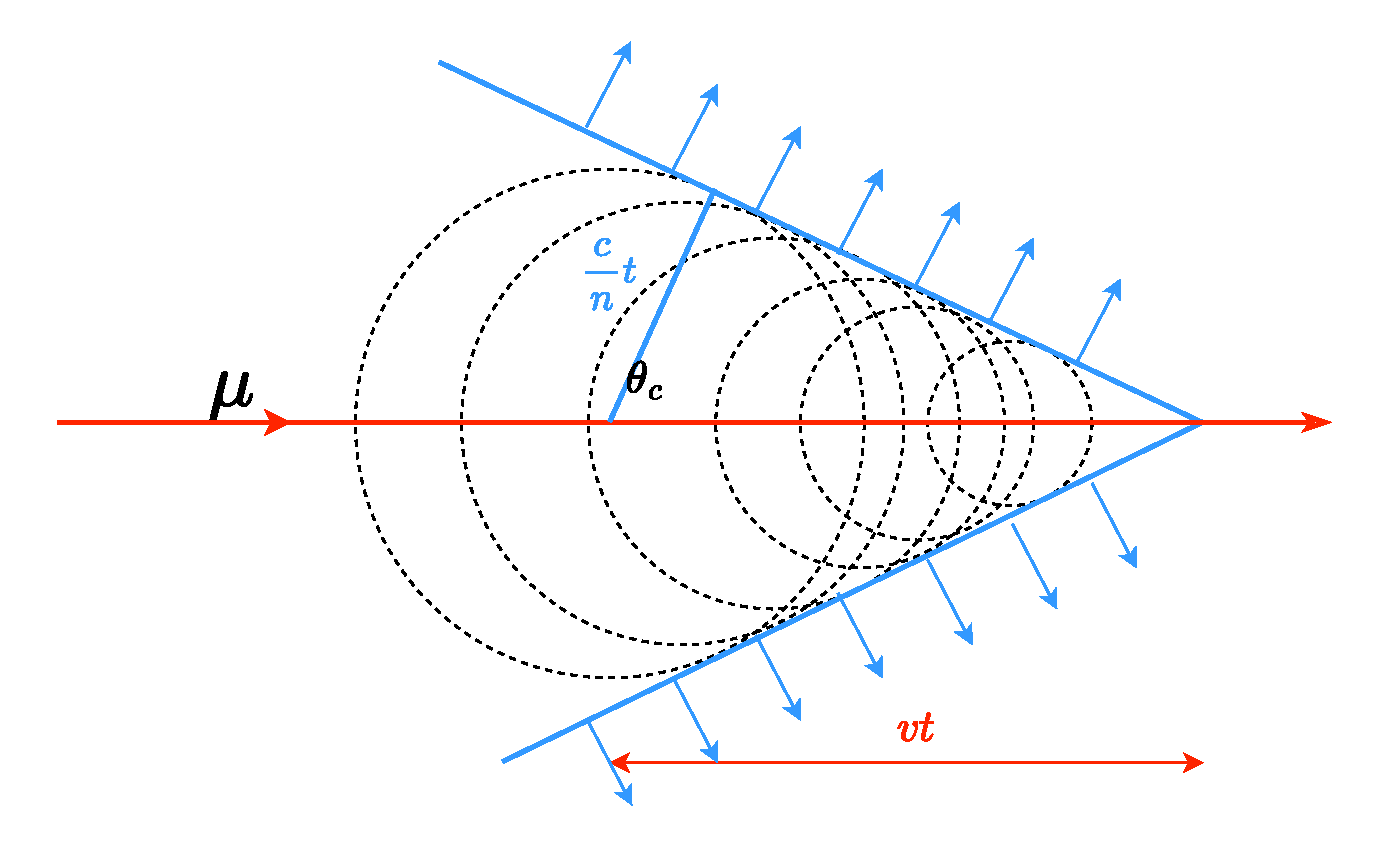
\includegraphics{./figures/nu_in_icecube/Cherenkov.pdf}
    \caption{The sketch shows the Cherenkov effect for a muon traveling through a dielectric medium with a velocity $v = \beta c$ (in red). The medium has a refractive index $n$, and the phase velocity of light $v_\mathrm{phase} = \frac{c}{n} $(in blue). The circles in the sketch represent wavefronts with equal phase shifts and illustrate isotropic and coherent emission (blue arrows) at an angle $\theta_c$ , for $v>v_\mathrm{phase}$.}
    \labfig{cherenkov}
\end{marginfigure}

When a charged particle moves through a medium at speed exceeding the phase velocity of light in that medium, it emits \emph{Cherenkov radiation} \sidecite{Cherenkov}, much like the shock wave generated by a supersonic jet. This radiation is emitted in a cone at an angle $\theta_C = \cos^{-1}\left(\frac{1}{\beta n}\right)$ relative to the particle's direction of travel, where $n$ is the refractive index of the medium and $\beta = \frac{v}{c}$ represents the ratio of the particle's velocity to the speed of light in a vacuum (see \reffig{cherenkov}). In ice, with a refractive index of $n = 1.31$ at a wavelength of 400 nm, which corresponds to the peak sensitivity of IceCube's optical modules (see, \ref{sec:dom}), the emission threshold for Cherenkov radiation is $\beta_\text{Ch} \gtrsim 0.76$. This corresponds to a minimum energy of 0.28 MeV for electrons and 58.09 MeV for muons, both of which are below IceCube's detection threshold of around 200 GeV. For high-energy particles in IceCube, where $\beta \simeq 1$, the Cherenkov cone's opening angle is $\theta_\text{Ch} \simeq 40.2^\circ$ at the peak sensitivity wavelength. The number of Cherenkov photons emitted within a waveband $d\lambda$ by a particle with charge $ze$ within the propagation length $dx$ is given by the Frank-Tamm formula \sidecite{Frank_Tamm}:

\begin{equation}\label{eq:cherenkov_ph}
    \frac{d^2N}{dxd\lambda} = \frac{2\pi \alpha z^2}{\lambda^2} \left( 1 - \frac{1}{\beta^2 n(\lambda)^2} \right)
\end{equation}
where, $\alpha$ is fine structure constant \sidecite{PDG_2024}. Using this formula, one can calculate that for a high-energy particle with $\beta \simeq 1$ passing through ice, approximately 250 photons/cm are emitted in the wavelength range of 300 nm to 500 nm, which is within IceCube's optimal detection range \sidecite{shower_profile}. 

Neutrino interactions in IceCube are detected indirectly through Cherenkov radiation from secondary charged particles (leptons, hadrons and electromagnetic showers, see \ref{sec:particle_propgation}) , reffered to as \emph{visible light} in IceCube. At energies above 1 TeV, the Cherenkov light from a muon itself becomes negligible, and detection primarily depends on light emitted by secondary particle showers along the muon's path. 

\subsection{Event Signatures}
\label{sec:morphologies}
The previous sections described the detector and its various components, along with the interactions and passage of neutrinos and the secondary particles they produce. In IceCube, events are visualized with the detector shown as an array of strings, with each colored sphere representing a triggered DOM. The sphere's size scales with the detected cherenkov light amount (charge accumulated), and its color indicates the arrival time. Section \ref{sec:DIS}, discussed how all-flavor neutral current (NC) interactions result in the transfer of a fraction of the neutrino's energy to the nucleus, initiating a hadronic shower. On the other hand, charged current (CC) interactions are accompanied by a charged lepton, whose propagation patterns were detailed in \ref{sec:leptons_inice}. The involvement of specific neutrino flavors in CC events leads to a distinct energy deposition patterns (\emph{morphology}), which can be used to identify the neutrino flavor. Additionally, when a neutrino interaction occurs within the volume of the detector, it is classified as a \emph{starting} event, and if the energy deposition is entirely within the detector volume, it is termed a \emph{contained} event.
Hadrons and electrons produce showers, which are known in IceCube as \textbf{cascades}. Due to the low radiation lengths of electrons and the short shower maximum caused by various secondary particles, cascades are contained within a few meters. This causes Cherenkov light emission to appear as a point-like source relative to the kilometer-scale detector. However, due to a higher scattering coefficient \ref{sec:icemodel} the light pattern appears almost spherical for cascades see \reffig{topologies}, due to which, the angular information is lost (or becomes less reliable) upon reaching the DOMs, leading to a poor angular resolution. In electromagnetic cascades, most of the interaction energy is contained within the cascade, making $\nu_{e}$ - CC events excellent candidates for energy estimation \sidecite{energy_reco}.
\begin{figure}
	\centering 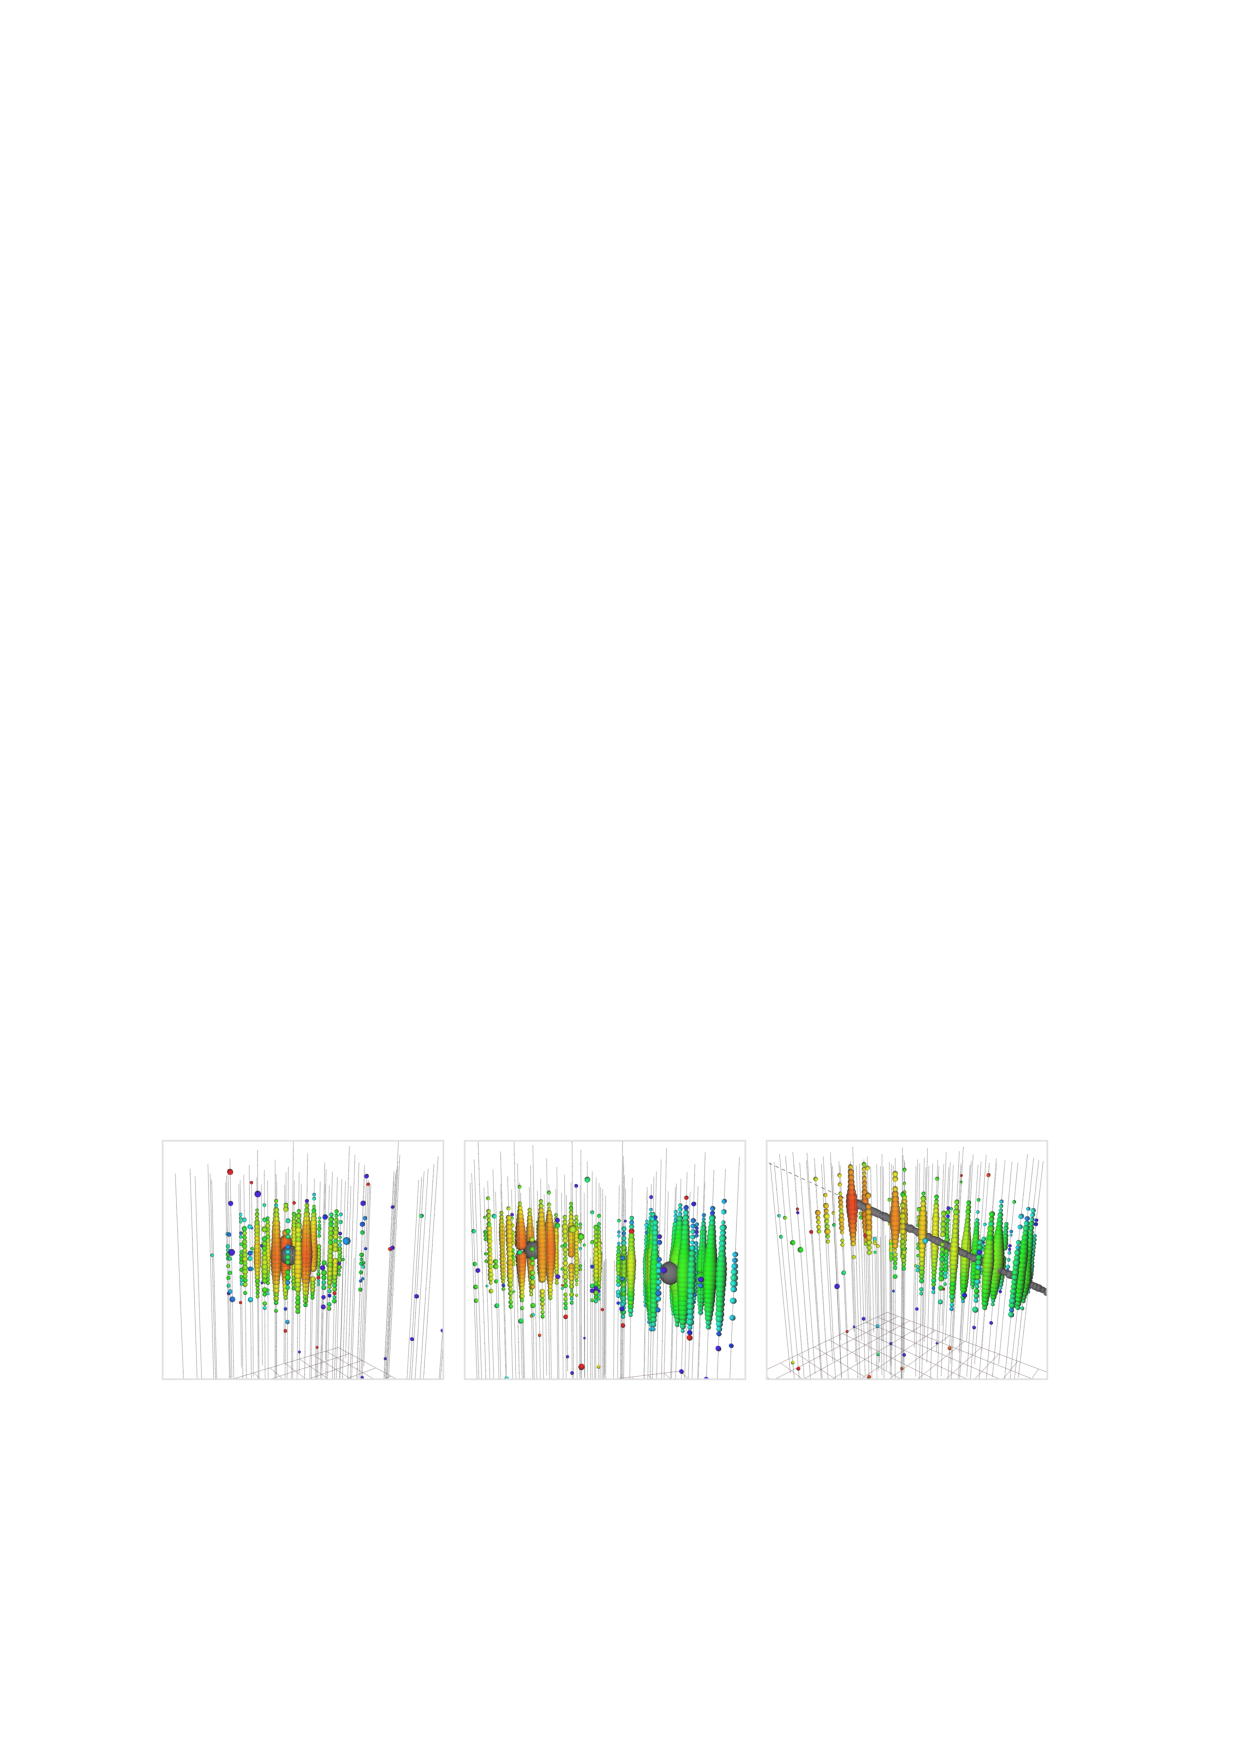
\includegraphics{./figures/nu_in_icecube/topologies.pdf}
	\caption{Simulated event signatures of single cascade (left), double cascade (middle), and track (right). Sizes of the spheres represent the amount of detected light, and colors show the photon arrival times. Single cascades are caused by electromagnetic and hadronic showers, double cascades by the production and decay of a tau lepton, and tracks by muons traversing the detector.}
    \labfig{topologies}
\end{figure}

\textbf{Tracks} are observed when highly energetic muons traverse the detector, most commonly from atmospheric muons produced by cosmic-ray-induced air showers. Tracks are also caused by CC interactions of $\nu_{\mu}$($\bar{\nu}_\mu$), which produce a hadronic cascade and a $\mu^-$ ($\mu^+$). When the neutrino interaction vertex is outside the detector volume, atmospheric muons and neutrino-induced muons are indistinguishable unless their energy and direction are considered\todo{is there any nu sources paper that can be cited for this claim?}, leading to \emph{a through-going track}. When the vertex is inside the detector volume, both the hadronic cascade and the emerging muon track are visible, resulting in \emph{a starting track}, which can only be caused by neutrino interactions. Although muons exhibit stochastic energy loss and are likely to exit the detector, resulting in poor energy resolution, the light deposition along an extended path (see \reffig{topologies}) provides good angular resolution (less than 1 degree), making tracks ideal for identifying high-energy astrophysical sources \cite{energy_reco}.

Tau neutrinos in IceCube exhibits variety of signatures, thanks to different tau decay modes (\ref{eq:tau_decay}). This leads to various event morphologies \sidecite{Tau_int_inice} based on factors like position of both, the neutrino interaction and tau decay verteces, decay channel and the decay length, as shown in \reffig{tau_morphologies}. The tau decay length ($\mathrm{L}_\tau$) is connected to Energy of tau lepton ($E_{\tau}$) via $\mathrm{L}_{\tau}\simeq\frac{50\mathrm{m}}{1\mathrm{PeV}}E_{\tau}$. $\nu_{\tau}$ CC events typically produce two energy depositions: an initial interaction cascade followed by a tau decay product, which can be a track or cascade, depending on the decay channel. The muonic decay channel results in a dim tau track followed by a brighter muon track.\footnote{The stochasticity of muon energy losses and the low branching ratio of the muonic decay channel (17.4\%) make it challenging to search for this signature. Therefore, this decay channel is excluded from the analysis presented in this thesis.} The other decay channels, involving hadrons or electrons, produce a cascade, leading to the so-called \textbf{double bang} events \sidecite{double_bang}. Around 59\% of tau-neutrino interactions are double bang events.\footnote{The muonic decay of the tau has a branching ratio of around 17\%, while all other decay channels of the tau produce another cascade with an inclusive branching ratio of approximately 83\%. When multiplied by the fraction of the charged-current cross-section over the total cross-section \cite{PDG_2024}, about 59\% of all tau-neutrino interactions are double bang events.}

\begin{figure}
	\centering 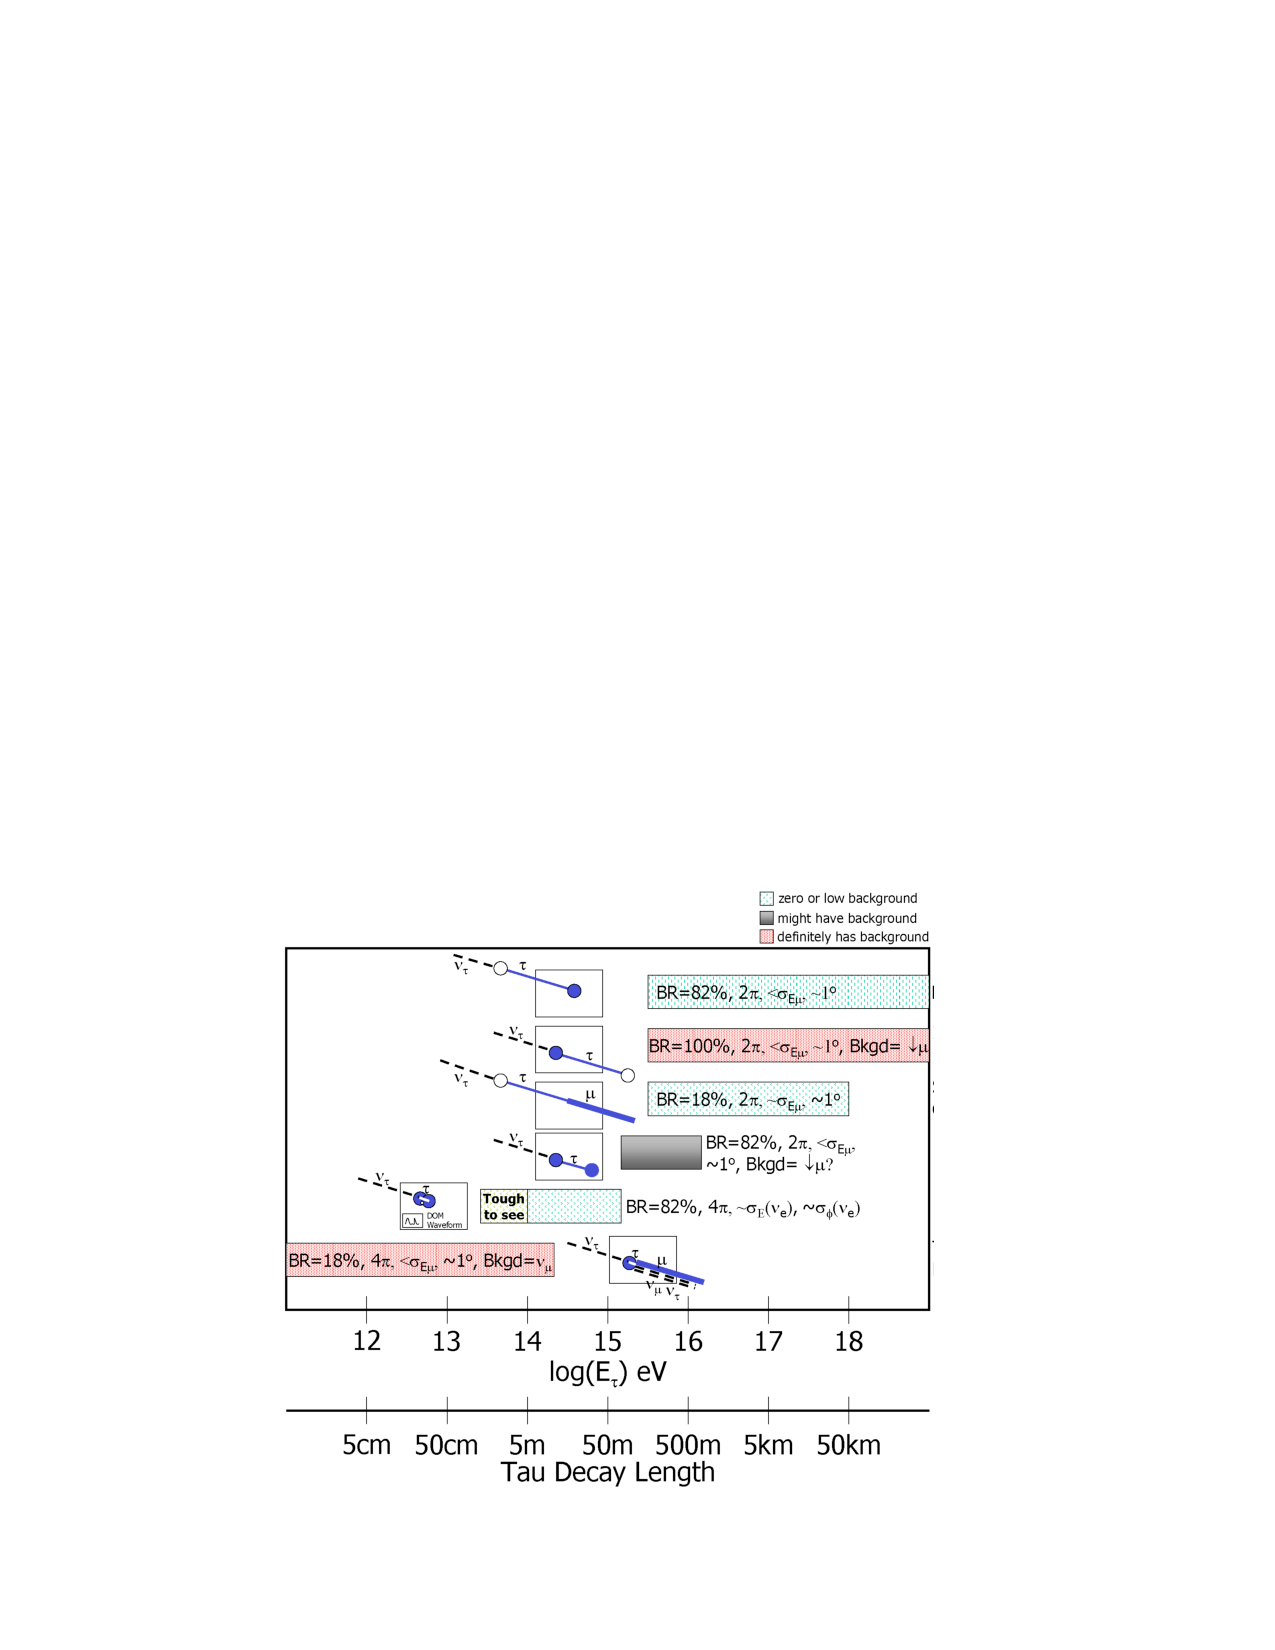
\includegraphics{./figures/nu_in_icecube/tau_interactions.pdf}
	\caption{Various morphologis of $\nu_{\tau}$ cc events in IceCube, as a function of $E_{\tau}$ and $\mathrm{L}_\tau$. Circle represent a cascade, dotted line represents primary $\nu_{\tau}$, thin line, Tau lepton track and thick line represent muon track.(Figure taken from \cite{Tau_int_inice})}
    \labfig{tau_morphologies}
\end{figure}

These double bang events are further classified based on whether both the interaction vertex and tau decay vertex are within the detector volume (see \reffig{tau_morphologies}). At lower energies (below $(\sim 100$) TeV), the separation between the two cascades is small, making them difficult to resolve. In some cases, if the event occurs close to a string or Digital Optical Module (DOM), two distinct time-connected pulses can be observed, known as the \textbf{double pulse} technique. However, identifying tau neutrino events in IceCube is challenging due to background muons and the difficulty in reconstructing such events. Recent developments using CNN classifiers have identified seven astrophysical tau neutrino candidates \sidecite{CNN_tau}. Lastly, if both of these caascades are contained in the active volume, and they are far enough to be reconstructed reliably, the morphology is called \textbf{double cascade}. This method has low and high tau energy threshold, since below certain energy ($\sim100$ TeV) the decay length is quite short, making them indistinugishable from a usual cascade event, and energies above 10 PeV, (where theoretically  the length should be  large enough to separate the two cascades) one of the cascades will always be outside the detector volume. In such case, a larger detector volume, such as in IceCube Gen2, could extend the energy range for identifiable double cascade events (see \refch{gen2}). 

The analysis performed in this thesis aims to measure neutrino flavour composiition where three of the morphologies explained above, starting tracks, double cascades and cascades (from hereon reffered to as single cascades, to differentiate from double) are used to identify flavour of the neutrino. Double cascades are not only challanging due to their tricky geometry but also because of involvement of both electromagnetic and hadronic particle showers involved. Lastly, as was discussed in \ref{sec:icemodel }the medium (ice) itself has many characteristic properties that affects the reconstruction of these events drastically. Details of sampling these high energy starting events and reconstructing them in to these three morphologies will be explained in the next chapter. 






% \begin{table*}[h!]
%     % \centering
%     \caption{Table showing the interaction types, flavors, morphologies, and containment types.}
%     \begin{tabular}
%     \hline
%     \textbf{Interaction Type} & \textbf{Flavor} & \textbf{Morphology} & \textbf{Containment Type} \\ \hline
%     \multirow{2}{*}{Neutral Current (NC)} & All & Hadronic Cascade & Starting, Contained \\  
%      &  &  &  \\ \hline
%     \multirow{10}{*}{Charged Current (CC)} & $\nu_e$ & Electromagnetic Cascade & Starting, Contained \\ \cline{2-4} 
     
%      & $\nu_\mu$ &  Track &  Starting\\ 
%      &  &  & Through-going \\ \cline{2-4} 
%      & $\nu_\tau$ & Tau Track & Starting, Contained \\ \cline{2-4} 
%      &  & Double Bang & Starting, Contained \\ \cline{2-4} 
%      &  & Dim Tau Track, Bright Muon Track & Starting, Contained \\ \cline{2-4} 
%      &  & Double Cascade & Starting, Contained \\ \cline{2-4} 
%      &  &  &  \\ \hline
%     \end{tabular}
    
% \end{table*}
    
\setchapterpreamble[u]{\margintoc}
\chapter{Event Sample and Reconstruction}
\labch{nu_samples}


\section{Detection of Neutrinos} 
\label{sec:nu_detection}
\setchapterpreamble[u]{\margintoc}
\chapter{Flavour Composition Analysis}
\labch{analysis}
Using the High Energy Starting Event (HESE) sample introduced in \refch{nu_samples}, that classifies high-energy neutrino events into one of three distinct morphologies (Single Cascades, Tracks and Double Cascades), a flavour measurement of the high energy diffuse neutrino spectrum can be performed. This chapter focuses on the methods and various ingredients used to make this flavour measurement. 

The chapter begins by detailing these statistical techniques, with a focus on forward folding likelihood fits, which plays a crucial role in distinguishing signal from background in measuring the flavour composition of the astrophysical neutrino flux. The modelling of signal and background events, enhanced for the iteration of this analysis performed in this thesis are explained subsequently. Finally, the chapter evaluates the sensitivity of the analysis, providing estimates of detection limits.
\section{Statistical Methods}
\label{sec:analysis}
This analysis utilizes a binned maximum likelihood estimation (MLE) approach to perform statistical inference based on the observed data. Binning the data offers computational efficiency as computing probability densities for an unbinned likelihood is not trivial in the case of finite MC statistics. One need to somehow parametrize them as a function of the signal and nuisance parameters. Forward-folding circumvents this by directly re-computing the distributions corresponding to a certain parameter set. Each analysis bin contains data points from a specific range of measured quantities, such as energy or angular distributions. To incorporate the complexities of detector response and model uncertainties, the concept of forward folding is employed. Forward folding integrates theoretical model predictions with the response of the detector, producing distributions of the expected event rate that can be directly compared to the binned observed data. This method allows for testing different flux models of arbitrary shape, along with the systematic uncertainties of these models as well as the detector responses, all folded into the predicted likelihood. 

\subsection{Binned Maximum-likelihood Fits}
\label{sec:MLE}
When fitting a data sample with a large size (large $N$), it is common practice to bin the data in order to enhance the computational efficiency of the likelihood function calculation. This binning procedure groups the data into discrete intervals, or \emph{bins}, based on one or more \emph{observables} (derived from reconstructed properties of the neutrino events), such as energy or zenith. This simplification is not harmful as long as the variation of the probability density function (PDF), $f(x|\theta)$, within each bin is insignificant compared to its variation across the neighbouring bins. In other words, the binning should not discard crucial information about the parameter vector $\theta$ that governs the underlying physical model. If a binning is applied appropriately, the fit retains the ability to accurately infer the parameters of interest while significantly speeding up the computational process, particularly in high-dimensional analyses where unbinned likelihood fits may be computationally prohibitive.

The binned likelihood method works by comparing the number of observed events in each bin to the expected number of events, which are typically predicted through Monte Carlo simulations. In the analysis, these Monte Carlo templates are created for various theoretical flux components, such as astrophysical, atmospheric etc. that constitute signal and background to the measurement. Each template provides a predicted event distribution based on specific values of the \emph{signal} parameters $\theta$ along with \emph{nuisance} parameters, $\xi$, which describe the physical processes being studied. These templates are obtained from forward folding, meaning they incorporate the effects of the detector response, before being compared to the observed data. By adjusting the model parameters, the predicted event counts in each bin can be varied to find the \emph{best fit} to the data. The number of observed events $n$, in each bin $i$ ($n_i$), is assumed to follow a Poisson distribution\sidenote{This is a good assumption because what we are doing here is essentially a counting experiment in every bin.} \sidecite{data_analysis_book}. The expected number of events in bin $i$, $\mu_i(\theta,\xi)$, represents the sum of contributions from all signal and background components. The Poisson likelihood for a given bin is defined as:

\begin{equation}\label{eq:Poisson}
    P(n_i|\mu_i(\theta,\xi)) = \frac{\mu_i(\theta,\xi)^{n_i} e^{-\mu_i(\theta,\xi)}}{n_i!}
\end{equation}

where $\mu_i(\theta,\xi)$ is the expected number of events in bin $i$ and $n_i$ is the observed number. The total likelihood for the entire dataset is then the product of the likelihoods for all bins:

\begin{equation}\label{eq:llh_noprior}
    \mathcal{L}(n|\mu_i(\theta,\xi)) = \prod_{i=1}^{N} P(n_i|\mu_i(\theta,\xi))
\end{equation}

Incorporating systematic uncertainties into the likelihood function is crucial for obtaining realistic results, as these uncertainties often arise from imperfect detector calibration or background estimations. Such systematic uncertainties are modeled as nuisance parameters in the likelihood fit. These parameters are typically constrained by prior knowledge and treated as additional variables in the fitting process. For each of the $k$ nuisance parameters, $\xi_j$, a Gaussian prior is introduced, penalizing deviations from the central value $\bar{\xi_j}$ by an amount proportional to the known uncertainty $\sigma_{\xi_j}$, extending the likelihood to:

\begin{equation}\label{eq:llh_withprior}
    \mathcal{L}(n|\mu_i(\theta,\xi)) = \prod_{i=1}^{N} P(n_i|\mu_i(\theta,\xi)) \prod_{j=1}^{k} \exp\left(-\frac{1}{2}\left(\frac{\xi_j - \bar{\xi_j}}{\sigma_{\xi_j}}\right)^2\right)
\end{equation}
By maximizing this likelihood, the best-fit parameters $\theta$ can be found. In practice, the fit is performed by minimizing $-\ln\mathcal{L}$, as it simplifies the computation (see \ref{eq:logllh}). 

\begin{equation}\label{eq:logllh}
    \ln(\mathcal{L}(n|\mu_i(\theta,\xi))) = \sum_{i=1}^{N} \left[ n_i \ln(\mu_i) - \ln(n_i!) - \mu_i \right] 
    - \sum_{j=1}^{k} \frac{1}{2} \left( \frac{\xi_j - \bar{\xi_j}}{\sigma_{\xi_j}} \right)^2
\end{equation}

Once the likelihood function is constructed, the next step is hypothesis testing. A specific model hypothesis can be tested by using a likelihood ratio test. The likelihood ratio compares two hypotheses: the test model (with parameters $\theta_t$) and the best-fit model (with parameters $\hat{\theta}$):

\begin{equation}\label{eq:llh_ratio_TS}
    -2 \Delta \ln \mathcal{L} = -2 \ln \left( \frac{\mathcal{L}(n|\mu(\theta_t, \xi_t))}{\mathcal{L}(n|\mu(\hat{\theta}, \hat{\xi}))} \right)
\end{equation}

The factor $-2$ is included for convenience, as the thus constructed test statistic follows a $\chi^2$ distribution under certain regularity conditions \sidecite{profile_llh}. Now, according to Wilks' theorem \sidecite{Wilks_thm}, this enables the calculation of confidence levels (CL) of the parameter of interest without the need for calculating the sampling distribution of $-2 \Delta \ln \mathcal{L}$ based on pseudo-experiments, which can be computationally expensive. However, Wilks’ theorem is only valid when the dataset is large and the model parameters are unbounded. If either condition is not met, the test statistic may deviate from a $\chi^2$-distribution, necessitating the use of Monte Carlo pseudo-experiments to determine the confidence intervals via the so-called \emph{Feldman Cousins} method \sidecite{feldman_cousin}, with an extension to incorporate nuisance parameters \sidecite{feldman_cousin_nuisance,asimov}.

The test statistic derived from the likelihood ratio, defined in Equation~\ref{eq:llh_ratio_TS} can be used to construct confidence regions for the parameters of interest, the process known as \textbf{a profile likelihood test}. For instance, in one-dimensional profile likelihood test, the confidence interval is obtained by comparing the test statistic to the cumulative distribution of a $\chi^2$-distribution with one degree of freedom. When scanning over two or more parameters, calculating the profile likelihood ratio on a multi-dimensional grid of parameter values is required, which significantly increases the computational complexity. In some cases, the Asimov dataset \cite{asimov}—a single dataset representing the median outcome of many pseudo experiments—can be used to estimate the median sensitivity of the analysis. This method provides an efficient way to estimate confidence intervals and test the sensitivity of the analysis without the need for exhaustive Monte Carlo pseudo-experiments. The Asimov dataset and Wilks' theorem are both used to derive the sensitivity of the analysis as presented in \ref{sec:sensitivty}. It is important to point out that the primary parameters of interest in this analysis are the astrophysical neutrino flavour fractions. 
The number of $\nu_{\tau}$ events, which provide the strongest constraint on astrophysical $\nu_{\tau}$ fraction in the flux, is small. Additionally, the flavour fractions in the likelihood fit are constrained to be non-negative always, therefore the applicability of Wilk's therom is evaluated as needed.

\subsection{SAY Likelihood}
\label{sec:SAY}

The likelihood construction described in section \ref{sec:MLE} relies on the Poisson likelihood, which assumes that the expectations for each bin, $\mu_i$, to be known exactly. This assumption holds when the Monte Carlo simulations used in generating the expected distributions have large statistics, so that the uncertainty on $\mu_i$ due to finite MC statistics is small compared to the uncertainty on the observed data counts. However, MC simulations inherently come with their own uncertainties due to finite statistics, particularly in highe energy bins where the difficulty to populate them becomes larger due to increase in computational costs.

In binned forward-folding fits, statistical inferences are made by comparing observed data counts in each bin to the expected counts derived from the simulations. As outlined in Equation~\ref{eq:Poisson}, the Poisson likelihood assumes that $\mu_i$, the expected value per bin, is well-determined. However, this is often not the case in analyses like the one performed in this thesis, where overall event rates are low, and individual bin expectations may fluctuate significantly due to limited MC statistics. This mismatch can lead to can lead to overconfident predictions if these fluctuations in $\mu_i$ are not correctly accounted for.

To address this issue, an extended form of the Poisson likelihood ($\mathcal{L}_{\mathrm{eff}}$), or the so-called \textbf{SAY likelihood}, is used in this analysis \sidecite{SAY}. This likelihood incorporates the uncertainty from the limited MC statistics and provides more appropriate coverage for parameter estimates based on this likelihood. Specifically, the distribution of MC event weights in each bin is modeled using a scaled Poisson distribution, which introduces an additional uncertainty term, $\sigma_j^2$, for each bin. This term depends on the weights $w_j$ of the simulated MC events $j$ in the $i$-th bin and is defined as:

\begin{equation}
\sigma_i^2 = \sum_{j} (w_j^i)^2
\end{equation}

This uncertainty term, $\sigma_i^2$, is larger in bins with low statistics, and smaller in bins with higher statistics, ensuring that fluctuations in low-stat bins are adequately covered. This formalism results in more conservative limits, with generally wider contours for the final result, as the additional statistical uncertainty is incorporated into the fit. One limitation of this approach is that the Asimov dataset \sidecite{asimov}, described in the previous section, cannot be constructed when using the SAY likelihood. This is because the $\sigma_j$ term can significantly skew the distribution $\mathcal{L}_{\text{eff}}(\mu_i | \sigma_i, d_i)$ so that the maximum is not at $\mu_i=d_i$, which is the defining property of the Asimov set. As a result, deviations from injected values may appear, especially in cases like the simulation produced for single atmospheric muons (\texttt{MuonGun}, explained in Section~\ref{sec:sim_ic}), which exhibits lack of high statsics due to high energy threshold of HESE sample, used in this work. Alternatively, the standard Poisson likelihood can be used, though the resulting limits may be overconfident.


\section{Components of the Likelihood Fit}
\label{sec:components}
The choice of the likelihood function and its subsequent requirements (the SAY likelihood)  was outlined in the previous section. In this section, the focus shall be on the essential components involved, and their modeling. The construction proceeds as follows:

\begin{enumerate}
    \item The parameters to be measured, known as \emph{signal parameters} (denoted by $\theta$), along with all \emph{nuisance parameters} ($\xi$), which may originate from uncertainties in the detector response or background modeling (such as atmospheric spectra), are identified and bounded where necessary.
    \marginnote{
        \begin{kaobox} 
        This is why a penalty term is introduced in the likelihood. A Gaussian prior prefers that the parameters remain within the $1\sigma$ prior region, penalizing the likelihood if the fit favors values outside this range. 
        \end{kaobox}}
    \item These parameters are applied in the form of the neutrino \emph{flux}, assigning each Monte Carlo event a specific \emph{weight} based on the individual fluxes.

    \item A set of observables that are most sensitive to the signal parameters, such as astrophysical neutrino fluxes, is selected and the simulated and experimentally observed events are accordingly binned for the analysis. The experiment is performed, and the observed data events $n$ are sorted into the predefined bins of the analysis histograms.
    \
    \item  A fit is conducted by varying each of the parameters (and, consequently, the fluxes) until the observed data events are optimally described. 
\end{enumerate}


\subsection{Model parameters}
\label{sec:params}
All the model parameters used in the fit, grouped by the flux component (astrophysical or atmopsheric) that they affect, are listed in \reftab{fit_params}. Moreover, several nuisance parameters describing uncertainty in the detector response are included in the fit. Baseline models and their corresponding values, wherever applicable, are specified for each parameter, along with the choice of priors. The astrophysical flux parameters represent the high-energy neutrino contributions from distant sources, while atmospheric flux models account for neutrinos originating from cosmic ray interactions within in atmosphere of Earth. 

\begin{table*}[h]
    \caption[The description of the parameters used in the likelihood fit, along with priors (if used)]{Parameters used in the likelihood desribed in Equation \ref{eq:llh_withprior}. The gaussian priors on the parameters (if applicable) in terms of the mean ($\mu$) and width ($\sigma$) are stated on the alongside.}
    \labtab{fit_params}
    
    \begin{tabular}{ |c |c|}
        \hline
        Parameter & Prior ($\mu,\sigma$)\\
        \hline
        \hline
        \multicolumn{2}{c}{\textbf{Astrophysical Flux (Signal) Parameters}}\\
        \hline
        astro. $\nu_{\mu}$ normalisation [$10^{-18} \mathrm{GeV}^{-1}\mathrm{cm}^{-2}\mathrm{sr}^{-1}\mathrm{s}^{-1}$]($\phi_{\nu_{\mu}}$) & - \\
        % \hline
        astro. spectral index ($\gamma_{\mathrm{astro}}$) & -\\
        % \hline
        scaling factor to modify total flux norm ($\Phi_{\nu+\bar\nu}^{\mathrm{astro}}$) relative to $\phi_{\nu_{\mu}}$ ($s_{\nu_e}$ astro. $\nu_{e}$)&- \\
        % \hline
        astro. $\nu_{\tau}$ scaling factor to modify total flux norm ($\Phi_{\nu+\bar\nu}^{\mathrm{astro}}$) relative to $\phi_{\nu_{\mu}}$ ($s_{\nu_{\tau}}$) & -\\
        \hline
        \multicolumn{2}{c}{\textbf{Atmospheric Flux Systematics}}\\
        \hline
        Conventional Flux normalisation ($\Phi_{\mathrm{conv}}$)  & (1.0,0.2)\\
        % \hline
        Prompt Flux Normalisation ($\Phi_{\mathrm{prompt}}$) &  - \\
        % \hline
        Interpolation between Cosmic Ray Models ($\xi_{\mathrm{CR}}$)  & (0,1)\\
        % \hline
        Cosmic Ray Spectral Index Shift ($\Delta\gamma_{\mathrm{CR}}$) &  (0,0.05)\\
        % \hline
        Barr-parameter modifying the pion-contribution ($H_{\mathrm{Barr}}$) & (0,0.15)\\
        % \hline
        Barr-parameter modifying the kaon-contribution ($W_{\mathrm{Barr}}$) & (0,0.40)\\
        % \hline
        Barr-parameter modifying the kaon-contribution ($Y_{\mathrm{Barr}}$)& (0,0.30)\\
        % \hline
        Barr-parameter modifying the kaon-contribution ($Z_{\mathrm{Barr}}$) & (0,0.12)\\
        % \hline
        Muon Flux Normalisation ($\Phi_{\mathrm{muongun}}$)  & (1,0.5)\\
        % \hline
        Scale factor for Neutrino Nucleon Inelasticity weight ($\mathrm{I}_{\mathrm{scale}}$) & (1,0.1)\\
        \hline
        
        \multicolumn{2}{c}{\textbf{Detector Systematics}}\\
        \hline
        Optical Efficiency of DOMs ($\eta_{\mathrm{domeff}}$) & (1.0,0.1)\\
        % \hline
        Ice Absorption Scaling ($\eta_{\mathrm{abs}}$)  & (1.0,0.05)\\
        % \hline
        Ice Scattering Scaling ($\eta_{\mathrm{scat}}$) & (1.0,0.05)\\
        % \hline
        Parametrization for refrozen icecolumn ($\eta_{\mathrm{h.ice-p0}}$)  & (-0.27,0.5)\\
        % \hline
        Parametrization for refrozen icecolumn ($\eta_{\mathrm{h.ice-p1}}$) & (-0.042,0.05)\\
        % \hline
        Ice Anisotropy Scaling ($\eta_{\mathrm{aniso}}$) &  -\\
        \hline
        \hline
    \end{tabular}
    
\end{table*}

\textbf{The flux of astrophysical neutrinos} is modeled as a single power law of the form
\begin{equation}\label{eq:SPL}
\Phi_{\nu + \bar{\nu}}^{\mathrm{astro}}(E_{\nu}) = \Phi_{\mathrm{0}}^{\mathrm{astro}} \times 
    (1 + s_{\nu_{e}} + s_{\nu_{\tau}}) \times
    \left( \frac{E_\nu}{\mathrm{100\,TeV}} \right)^{-\gamma_{\mathrm{astro}}}
\end{equation}
where $\gamma_{\mathrm{astro}}$ is the spectral index, $E_\nu$ is the neutrino energy, and $\Phi_{\nu + \bar{\nu}}^{\mathrm{astro}}$ is the all-flavour (including particle and anti-particle) normalization. Two scaling factors, $s_{\nu_{e}}$ and $s_{\nu_{\tau}}$, modify the flux of electron and tau neutrinos relative to the muon neutrino flux $\Phi_{\mathrm{0}}$. These scaling factors relate to the flavour ratio $f_{\nu_e}:f_{\nu_{\mu}}:f_{\nu_{\tau}}$ as:

\begin{equation}\label{eq:flav_frac}
    \begin{array}{rcl}
        f_{e} = \frac{s_{\nu_{e}}}{(1 + s_{\nu_{e}} + s_{\nu_{\tau}})}, \quad
        f_{\mu} = \frac{1}{(1 + s_{\nu_{e}} + s_{\nu_{\tau}})}, \quad
        f_{\tau} = \frac{s_{\nu_{\tau}}}{(1 + s_{\nu_{e}} + s_{\nu_{\tau}})}
    \end{array}
\end{equation}

The signal parameters for the flavour analysis are these two scaling factors, $\Phi_{\mathrm{0}}$, and $\gamma_{\mathrm{astro}}$. All other subsequent parameters explained are the nuisance parameters. In Eq.~\ref{eq:SPL}, it is assumed that each flavour has an identical spectral shape ($\gamma_{\mathrm{astro}}$). This assumption is justified because the HESE sample used in this analysis is small and has limited power to constrain spectral properties resolved by neutrino flavour. For the sensitivity study described in \ref{sec:sensitivity}, the benchmark spectral parameter values are taken from the previous iteration of this analysis \sidecite{HESE7_sample}, with $\gamma_{\mathrm{astro}} = 2.87$ and $\Phi_{\mathrm{0}} = 2.12 \times 10^{-18} \mathrm{GeV}^{-1}\ \mathrm{cm}^{-2}\ \mathrm{sr}^{-1}\ \mathrm{s}^{-1}$ assuming an equipartition of flavour ratios (i.e., $\nu_e : \nu_{\mu} : \nu_{\tau} = 1:1:1$).

\textbf{Atmospheric flux components} are constrained by priors because they are more accurately measured with other IceCube data samples. In contrast, the number of atmospheric events in the HESE selection is low due to the high efficiency in reducing atmospheric muons due to the veto requirement and the down-going atmospheric neutrinos from the same cosmic-ray-induced air shower, thanks to the self-veto effect.

Depending on the parent hadron type, the atmospheric neutrino flux is divided into two components: \textbf{The Conventional neutrino flux} (produced in the decay of charged pions and kaons) and \textbf{The Prompt Neutrino Flux} (produced in the decay of charmed mesons). The various models of atmospheric neutrino fluxes are detailed in \ref{sec:atm_nu}. The atmospheric neutrino flux contribution is modeled using the Matrix Cascade Equation Solver (MCEq) \sidecite{MCEq}. The baseline primary cosmic-ray model for this calculation is H4a \sidecite{gaisser_H4a}, combined with a hadronic interaction model \texttt{SIBYLL2.3c} \sidecite{SIBYLL23c}, introducing conventional ($\Phi_{\mathrm{conv}}$) and prompt ($\Phi_{\mathrm{prompt}}$) flux normalizations to account foverall flux level uncertainties. Additionally, they are folded with the generalized self-veto probability, as described in \ref{sec:HESE}, to account for the reduced rate of atmospheric neutrinos accompanying vetoed muons from the same cosmic-ray-induced air shower. Other nuisance parameters modifying the shape of these spectra include $\xi_{\mathrm{CR}}$, which interpolates between two primary cosmic-ray models H4a and GST, an approach introduced in \sidecite{diffusenumu}. The cosmic-ray model uncertainty is the largest source of uncertainty in the overall atmospheric background. Furthermore, $\Delta\gamma_{\mathrm{CR}}$ accounts for corrections in the spectral index of the primary cosmic-ray spectrum, see for e.g. \sidecite{hans_thesis}. Uncertainties in the hadronic interaction models, due to various $\pi$ and $K$ production cross-sections in different energy phases, introduce energy-dependent variations in atmospheric flux expectations \sidecite{Barr}. These nuisance parameters, referred to as \emph{Barr} parameters, are computed as described in \sidecite{Anatoli_HI_model}. A detailed discussion on implementing these parameters within the software framework can be found in \sidecite{richard_thesis}.

As mentioned, the veto and charge/energy cuts effectively reduce the rate of atmospheric neutrinos. However, high-energy single muons can still enter the detector, contaminating the sample. \textbf{The atmospheric Muon Flux} component is constrained by a prior partially derived from experimental data. The spectral shape is determined using a dedicated simulation that produces a flux of single muons reaching the detector (\texttt{MUONGUN}, described in \ref{sec:mc_sim}), weighted assuming the same baseline models used for atmospheric spectra (H4a). A pure-proton composition is chosen for these muons as it contributes the highest energy single muons. The normalization is estimated using the tagging method described in \cite{HESE7_sample}. A separate nuisance parameter, $\Phi_{\mathrm{muongun}}$, is included in the fit to account for these muons. A prior derived from this study is applied in this analysis. The sensitive energy range of this analysis is high, and the sample is specifically designed to minimize background contamination from atmospheric neutrinos and muons (see Section \ref{sec:HESE}). The available \texttt{MUONGUN} Monte Carlo was generated for various other IceCube analyses, that targeted lower energies as well, where background contributions are significantly higher. Most Monte Carlo events do not pass the strict cuts of this analysis, with no events at all in the cascade and double cascade bins (see \reffig{cascade_mc} and \reffig{double_mc}). Consequently, the statistical uncertainty on this component is high, requiring a Kernel Density Estimate (KDE) for smoothing.

The remaining nuisance parameters are those arising from the imperfect knowledge of the detector response, such as the Digital Optical Modules (DOMs, see section \ref{sec:DOM}), and the detection medium, which includes both the bulk ice and hole ice models (see section \ref{sec:icemodel}), denoted as from here-on as \textbf{Detector Systematics}. These detector systematics introduce uncertainties that can affect both the energy scale of the neutrino events and the shape of observable distributions, thereby altering the expected event rates from different flux components. Unlike previous iterations of this analysis \sidecite{marcel_thesis,Juliana_thesis}, which relied on discrete Monte Carlo simulation sets with different values for systematics that significantly impacted the analysis observables, the current approach uses the SnowStorm simulation technique (see section \ref{sec:snowstorm}). The SnowStorm method \sidecite{snowstorm} captures the full range of detector systematic variations in a single Monte Carlo dataset, avoiding the need for generating multiple datasets. It uses a first-order Taylor expansion of the observables, such as event counts in each bin, with respect to the detector systematics. The resulting gradient, called \emph{the nuisance gradient} ($\vec{G}$), allows for efficient computation of observable values as these systematic parameters vary. The expectation value of per bin event count $\mu$, for nuisance parameter variations $\vec{\eta}$ is given as,

\begin{equation}\label{eq:gradient}
    \mu(\vec{\eta})  = \mu_{\mathrm{baseline}} + \vec{\eta}.\vec{G}
\end{equation}

where, $\mu_{\mathrm{baseline}}$ is the expectation value of per bin count at basleine values of all detector systematic parameters (baseline values are the central value at which simulation was generated), when $\vec{\eta}=\vec{0}$. For this approach to be valid, it assumes that systematic effects are small enough to be treated perturbatively, allowing for a linear approximation. By marginalizing over the full ensemble of systematic variations, the prediction converges to that of the central model, effectively neglecting second-order effects. Because the dataset itself have finite statistics, appropriate uncertainty propagation is applied to the nuisance gradient (see \sidecite{richard_thesis} for details of calculations of this gradient, their uncertainties and incorporation within such fits). 

For each analysis bin, both the expected number of events ($\mu_i$) and the associated variance ($\sigma_i$) are computed, that enter the likelihood calculation, described in Equation~\ref{eq:logllh}. However, two important caveats should be noted with this method. First, the gradients are calculated based on a specific flux assumption\sidenote{For the analysis presented in this thesis, the gradients are computed using the best-fit values from the HESE-7.5 year analysis \cite{HESE7_sample}, with $\gamma_{\mathrm{astro}}=2.87$, the per-flavour flux normalization $\Phi_{\nu + \bar{\nu}}^{\mathrm{astro}}=2.12$, and an equipartition among all three flavour fluxes.} and are not recalculated at every minimization step. This significantly reduces the computational time of the minimization process but may introduce inaccuracies if the assumed fluxes deviate significantly from the true values in nature, which could substantially alter the resulting gradients. A potential solution is to compute the gradients over a range of flux assumptions to check for significant deviations in the results. For the analysis presneted in this thesis, this was tested by varying single-power law paramters (index and normalisation) defined in Equation~\ref{eq:SPL}, in appropriate range\sidenote{The appropriate range here refers to a set of spectral measurements made by various IceCube samples \cite{diffusenumu,cscd_6yr,HESE7_sample,ESTES}.} and the results ensured that this was a higher order effect. The second caveat arises because the expected event counts per bin, calculated using the gradients as shown in Equation \ref{eq:gradient}, are applied as an \emph{additive} correction to the overall flux expectation. Since the gradient is a real valued vector, it can also take negative values. For softer spectra and the limited statistics of the HESE sample, this can result in negative bin counts when the expected values approach zero. This presents a problem for the likelihood fit used in the analysis, as the logarithm of a negative number\sidenote{also, a negative number of expected events is unphysical anyway!} cannot be computed (which the fitter will attempt to do at some point; see Equation~\ref{eq:logllh}). To avoid this numerical issue, the expectation value calculated via the gradients is clipped at $\mu = 0 + \epsilon$. This ad hoc correction is justified because, although $\mu_{\mathrm{baseline}}$ may be zero in these bins, there remains significant statistical uncertainty, which typically dominates over the systematic variations.

The aforementioned gradient, can be constructed using 6 detector systematics simulated within the snowstrom ensemble. For the analysis presented in this thesis, it is constructed using 6 parameters, listed in the \reftab{fit_params}. 
\begin{description}
    \item [\textbf{The DOM Efficiency ($\eta_{\mathrm{domeff}}$)}] accounts for factors like the quantum efficiency of the PMT and shadowing by attached cables, reducing the efficiency by 1\%. The overall uncertainty is estimated at $\pm10\%$ \sidecite{spicemie}. This impacts the reconstructed energy, as lower efficiency underestimates the photon light yield. This effect is relevant in the analysis, as it shifts the energy distribution across bins and the energy thresholds in particular.
    \item [\textbf{Absorption ($\eta_{\mathrm{abs}}$) and Scattering ($\eta_{\mathrm{scat}}$) Scaling}] accounts for variations in scattering and absorprion coefficients of the ice model, mapped across a depth grid of the south pole ice. The baseline model for this mapping is SPICE-3.2.1, with priors set to a 5\% width around the central value, based on the uncertainty derived from calibration data obtained using flasher LEDs \cite{spicemie}. An increase in scattering coefficients extends the photon scattering path, increasing the chance of absorption before detection. Variations in ice scattering and absorption mainly affect energy reconstruction and may introduce minor directional bias, with the energy shift being the primary concern in this analysis.  
    \item [\textbf{hole ice parameters ($\eta_{\mathrm{h.ice-p0}}$ and $\eta_{\mathrm{h.ice-p1}}$)}] accounts for the differences in optical properties between the refrozen ice in the DOM deployment columns and the surrounding bulk ice. Uncertainties and priors are based on a recent study that analyzed flasher data \sidecite{holeice_eller_icrc23}.
    \item [\textbf{Ice anistropy}] discussed in detail in sections \ref{sec:icemodel} and \ref{sec:icemodel_checks} affects the double cascade reconstruction greatly. For the ice model used in simulation, this parameter is modelled as a modulation of the nominal scattering coefficient, analogous to that used in \sidecite{Juliana_paper}.
\end{description}



Lastly, an additional nuisance parameter, affecting the DIS neutrino interaction cross section (discussed in Section~\ref{sec:DIS}) and thus all the neutrino fluxes (Astrophysical and atmospheric) is used. The so-called \textbf{Neutrino-Nucleon Inelasticity Scaling ($\mathrm{I}_{\mathrm{scale}}$)} parameter is introduced to account for  inelasticity which is a measure of the fraction of the neutrino's energy that is transferred to the hadronic system in an inelastic neutrino nucleon scattering process, mathematically given as,
\begin{equation}
     y  = \frac{E_{\text{hadron}}}{E_\nu}
\end{equation}
The Mean inelasticity $\langle y \rangle$ is the average value of the inelasticity $y$ over many scattering events. It provides a statistical measure of the average fraction of the neutrino's energy that is transferred to the hadronic system. This is particularly relevant for starting tracks, as the mean inelasticity, \(\langle y \rangle\), depends on the incoming neutrino energy. Since \(\langle y \rangle\) evolves as a function of energy (see Section~\ref{sec:inelasticity}), it indicates the fraction of the neutrino's energy transferred to the hadronic system during the \(\nu_{\mu}\) charged-current (CC) interaction. Consequently, this also determines how much energy is imparted to the muon in starting tracks. Thus, variations in \(\langle y \rangle\) with energy influence the overall energy distribution of the events. For this analysis, a scaling factor is introduced, which is based on formulation provided in \sidecite{gary_paper}, that allows to vary Normalisation $N$ of the inelasticity distribution, 
\begin{equation}
    \frac{dp}{dy} = N \left( 1 + \epsilon (1 - y)^2 \right) y^{\lambda - 1}
\end{equation}
where N is the normalisation given as,
\begin{equation}\label{eq:inel}
    N = \frac{\lambda (\lambda + 1) (\lambda + 2)}{2\epsilon + (\lambda + 1) (\lambda + 2)}
\end{equation}

The theoretical prediction of \(\langle y \rangle\) from the CSMS model \sidecite{CSMS} is calculated for the mean inelasticity distribution for a given event. By fixing \(\langle y \rangle\), $\lambda$ \ref{eq:inel} is the fitted to apply a reweighting factor to \textit{scale} the inelasticity ($\mathrm{I}_{\mathrm{scale}}$). Variations are permitted within 10\% of their default value. The parameter is applied to all neutrino fluxes as via Deep Inelastic Scattering.

\subsection{Analysis Observables and their Distributions}
\label{sec:hists}

In forward folding fits, selecting appropriate observables is crucial for distinguishing between the signal and background hypotheses. The analysis uses all the HESE events above 60 TeV, further divided in 3 sub-samples of \emph{Single Cascades, Tracks and Double Cascades}. These 3 sub-samples are binned in 2-dimensional Monte Carlo templates of appropriate observables, such that bakground and signal templates are clearly distingishabe. When measuring the spectrum of astrophysical neutrinos, the background consists of neutrinos produced in atmospheric air showers. Key observables that allow for effective differentiation between astrophysical and atmospheric neutrinos include the total deposited energy ($\mathrm{E}_\mathrm{tot}$) and the zenith angle ($\theta_{\mathrm{zenith}}$) of the interacting neutrino. The motivation for focusing on these variables stems from their distinct behavior in atmospheric and astrophysical neutrino spectra (see Section~\ref{sec:atm_nu}). In particular, down-going atmospheric neutrinos are efficiently suppressed due to the self-veto effect, while up-going atmospheric neutrinos, which cannot be reduced by this veto, become an irreducible background. 

\marginnote{
        \begin{kaobox} 
        The astrophysical spectrum that is assumed for all the Monte Carlo templates and sensitivity is using a single-power law based on best-fit values of HESE-7.5 years spectrum measurements \cite{HESE7_sample}, given as,
            \begin{equation}\label{eq:SPL}
                \frac{d\Phi_{\nu + \bar{\nu}}^{\mathrm{astro}}}{dE} = 6.98.10^{-18}\left( \frac{E_{\nu}}{100 \, \text{TeV}} \right)^{-2.87} 
            \end{equation}
        In units of $\text{GeV}^{-1} \, \text{cm}^{-2} \, \text{s}^{-1} \, \text{sr}^{-1}$, with flavour composition of $\nu_e:\nu_{\mu}:\nu_{\tau}=1:1:1$
        \newline
        The prompt component is missing from all templates as best-fit value of $\Phi_{\mathrm{prompt}}$ of prompt flux normalization was 0. 
        \end{kaobox}
}
For the analysis presented in this thesis, the primary goal is to measure the flavour composition of astrophysical neutrinos. A key component of this analysis, as highlighted in Section~\ref{sec:PID}, is the identification and classification of $\nu_\tau$-induced double cascade events. Note that the PID assigned is not used as a proxy to tag flavour on an individual event bases, but through statistical analyses of the overall data set, Monte Carlo templates. Double cascades are a signature of $\nu_\tau$ interactions, and their identification relies heavily on the observables $\mathrm{E}_\mathrm{tot}$ and the reconstructed double cascade length ($\mathrm{L}_{\text{dc}}$), which provide the most discriminatory power for separating the flavours of astrophysical neutrinos, see \reffig{LvsE_signalbkg}. All double cascade events are binned into a two-dimensional Monte Carlo template, with one axis representing the reconstructed tau decay length ($L_{\text{dc}}$) and the other representing the reconstructed total deposited energy ($E_{\text{Tot}}$). The $L_{\text{dc}}$ is divided into 10 bins ranging from 10 m to 1000 m, while $E_{\text{Tot}}$ is divided into 13 bins spanning 60 TeV to 12.6 PeV, both using logarithmic spacing, as shown in ~\reffig{LvsE_signalbkg}. It is important to note that adding a third dimension, such as energy asymmetry, offers significant discriminatory power by reducing the low-length single cascade background, enhancing the sensitivity to measure the flavour ratio \sidecite{Neha_ICRC_IC}. However, a detailed study revealed that the limited Monte Carlo statistics and small small size of the HESE sample resulted in many empty bins, which posed challenges for forward-folding fits. As a result, the third dimension was ultimately excluded from the analysis.


\begin{figure*}[h!]
    \begin{subfigure}[h]{0.72\textwidth}
        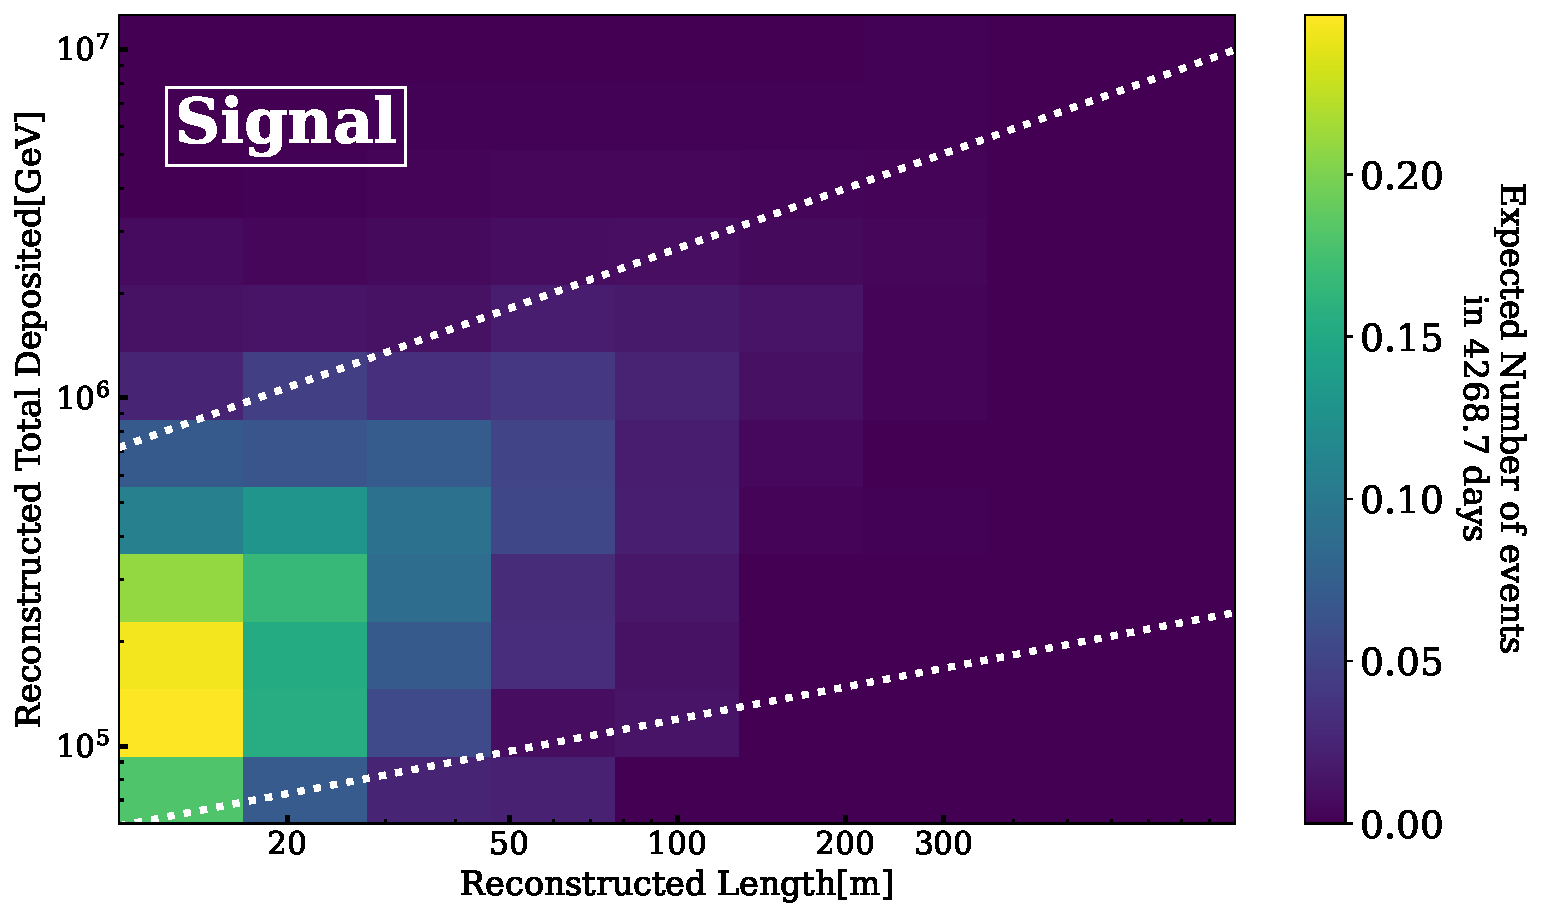
\includegraphics{./figures/Analysis/LvsE_signal.pdf}
    \end{subfigure}
    \hfill
    \begin{subfigure}[h]{0.72\textwidth}
        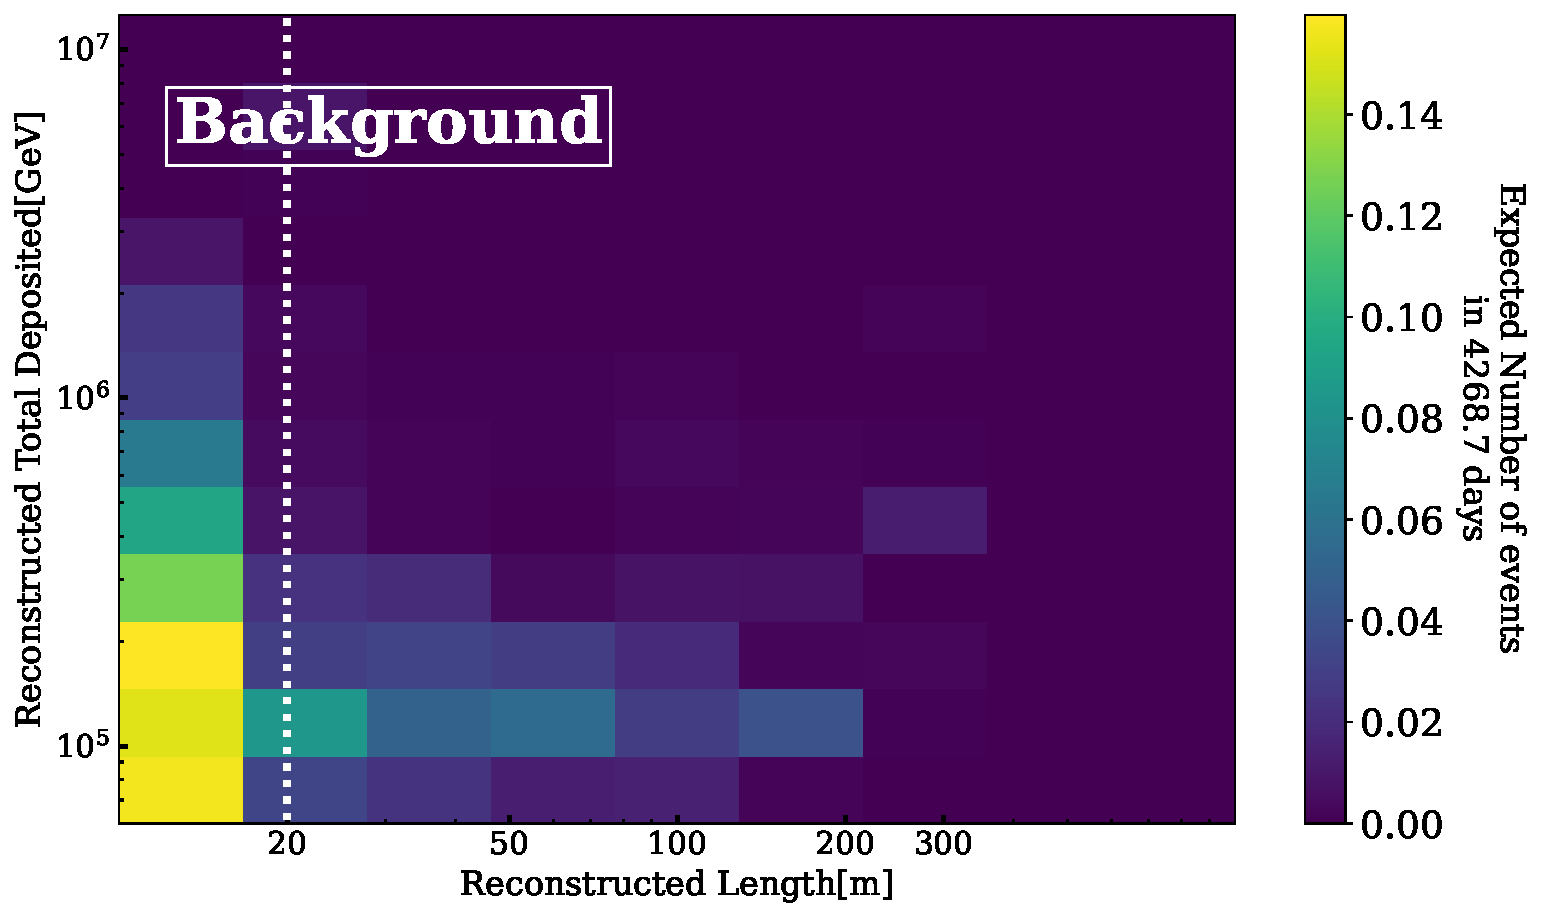
\includegraphics{./figures/Analysis/LvsE_Bkg.pdf}
       
    \end{subfigure}%
    \caption[Correlation of total deposited energy and length in 2D MC PDF, for signal and background double cascades]{2D Monte Carlo templates, constructed using reconstructed total energy ($E_{\text{Tot}}$) and double cascade length ($L_{\text{dc}}$) for events classified as \textbf{double cascades}. The signal (left), representing $\nu_\tau$-induced double cascades, shows a clear correlation between $L_{\text{dc}}$ and $E_{\text{tot}}$, with 68\% of events within the indicated signal region (dotted white line). In contrast, the background (right), consisting of $\nu_\mu$ and $\nu_e$ events, lacks this correlation and clusters at low $L_{\text{dc}}$, 68\% of all the background events lying below the indicated white dotted verticle line.}
    \labfig{LvsE_signalbkg}
\end{figure*}

Under the double cascade hypothesis, true single cascades are typically reconstructed with a small $\mathrm{L}_{\mathrm{dc}}$ but with most of their energy concentrated in the first cascade (with the energy asymmetry $E_A \rightarrow 1$). Hence, misclassified single cascades tend to cluster around low $\mathrm{L}_{\mathrm{dc}}$ and low $\mathrm{E}_{\mathrm{Tot}}$, with the distribution of $\mathrm{L}_{\mathrm{dc}}$ falling off rapidly, as indicated by the verticle line, on right panel of \reffig{LvsE_signalbkg}. In cases where a track is reconstructed under the double cascade hypothesis, the largest energy depositions are interpreted as the cascade vertices, leading to an arbitrary $\mathrm{L}_{\mathrm{dc}}$ value. These tracks, when misclassified as double cascades, typically exhibit low $\mathrm{E}_{\mathrm{Tot}}$, consistent with the falling astrophysical spectrum. This is also visible in right panel of \reffig{LvsE_signalbkg}.

True double cascades from $\nu_\tau$-CC interactions, on the other hand, exhibit a strong correlation between $\mathrm{L}_{\mathrm{dc}}$ and $\mathrm{E}_{\mathrm{Tot}}$. This correlation between $\mathrm{L}_{\mathrm{dc}}$ and $\mathrm{E}_{\mathrm{Tot}}$ is primarily used to determine the compatibility of an event with a $\nu_\tau$ interaction as opposed to another flavour. The Monte Carlo distributions (PDFs) of $\nu_\tau$-induced double cascades clearly show this correlation (see left panel of \reffig{LvsE_signalbkg}, indicating 68\% region of all classified true double cascade events). 

For single cascades and tracks, the observables $\mathrm{E}_{\mathrm{Tot}}$ (21 bins from 60TeV to 12.6 PeV in log space) and $\cos(\theta_z)$ (10 bins from -1 to 1 in cosine space) are commonly used, as they offer the most significant discrimination between astrophysical and atmospheric neutrinos, as shown in ~\reffig{cascades_2d} for cascades and ~\reffig{tracks_2d} for tracks. In both Figures, the supression of atmospheric neutrinos (right panel) ($\cos(\theta_z)$>0.25, the so-called \emph{down-going region} in IceCube) is clearly visible due to the self-veto effects, whereas astrophysical template (left panel) shows no such pattern\sidenote[-7cm]{Looking at the plot, it is not entirely true, as we do observe more events in the downgoing region $\cos{(\text{zenith})}\geq0.5$ because the up-going region requires a neutrino to travel much large distances through earth, and hence only a handful of neutrinos at high energies can do so.}, indicating neutrinos from all directions are accepted. 

\begin{figure*}[h!]
    \begin{subfigure}[h]{0.72\textwidth}
        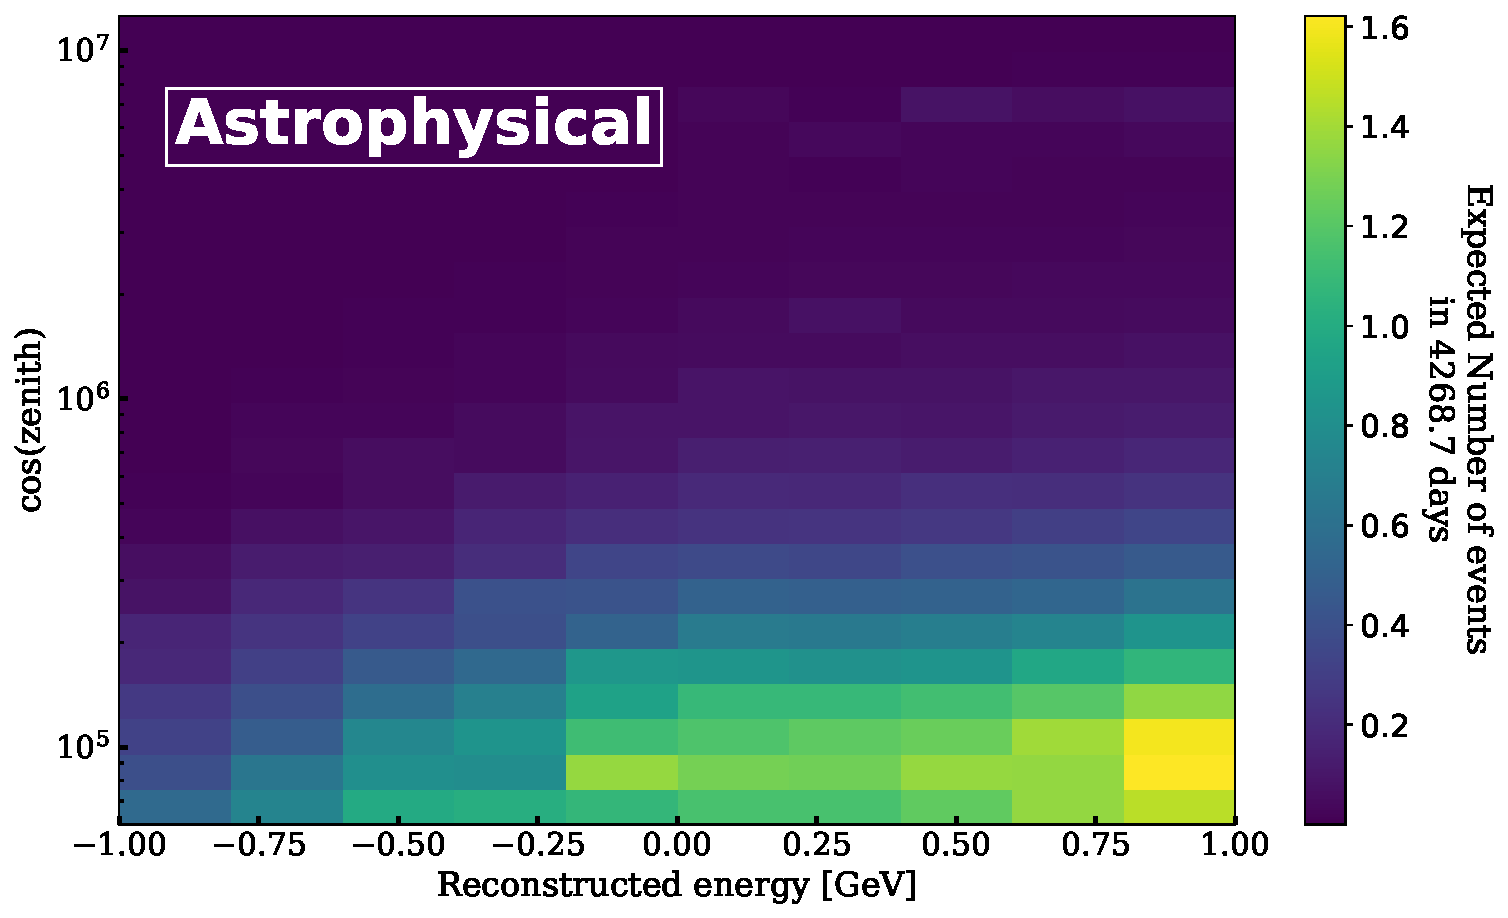
\includegraphics{./figures/Analysis/Cascades_Astrophysical.pdf}
    \end{subfigure}
    \hfill
    \begin{subfigure}[h]{0.72\textwidth}
        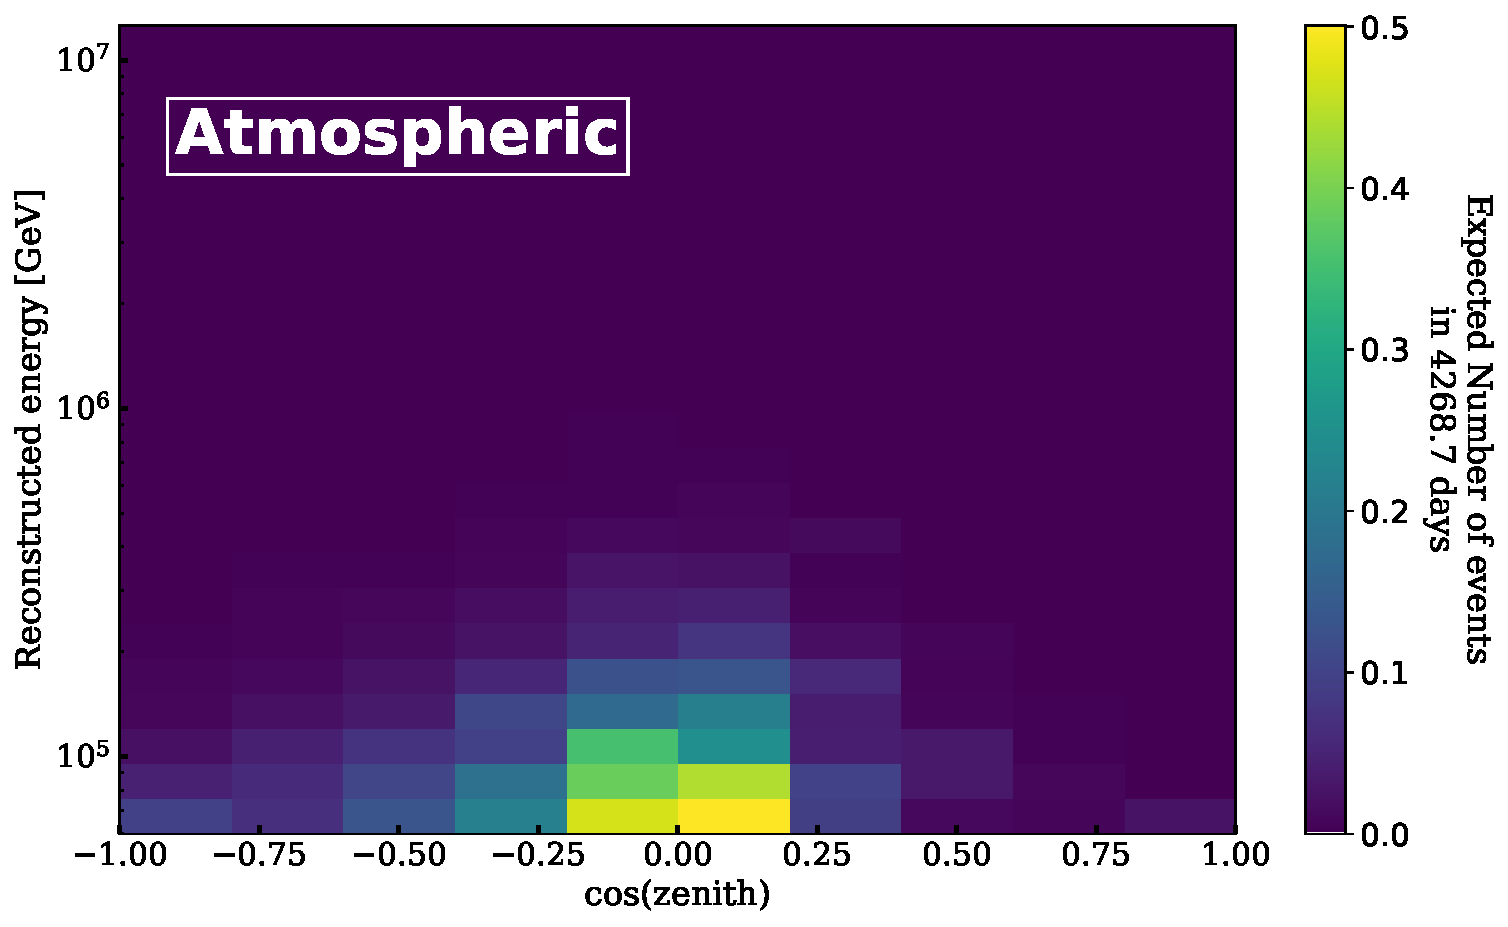
\includegraphics{./figures/Analysis/Cascades_Atmospheric.pdf}
       
    \end{subfigure}%
    \caption[2D Monte Carlo templates for cascade sample for astrophysical and atmopsheric fluxes]{2D Monte Carlo templates, constructed using reconstructed total energy ($E_{\text{Tot}}$) and reconstructed zenith ($\cos(\theta_z)$) for events classified as \textbf{single cascades}. The signal (left), representing \emph{Astrophysical neutrinos} of the sample and the background (right), representing \emph{Atmospheric neutrinos}, including conventional, prompt and single muon fluxes.}
    \labfig{cascades_2d}
\end{figure*}

\begin{figure*}[h!]
    \begin{subfigure}[h]{0.72\textwidth}
        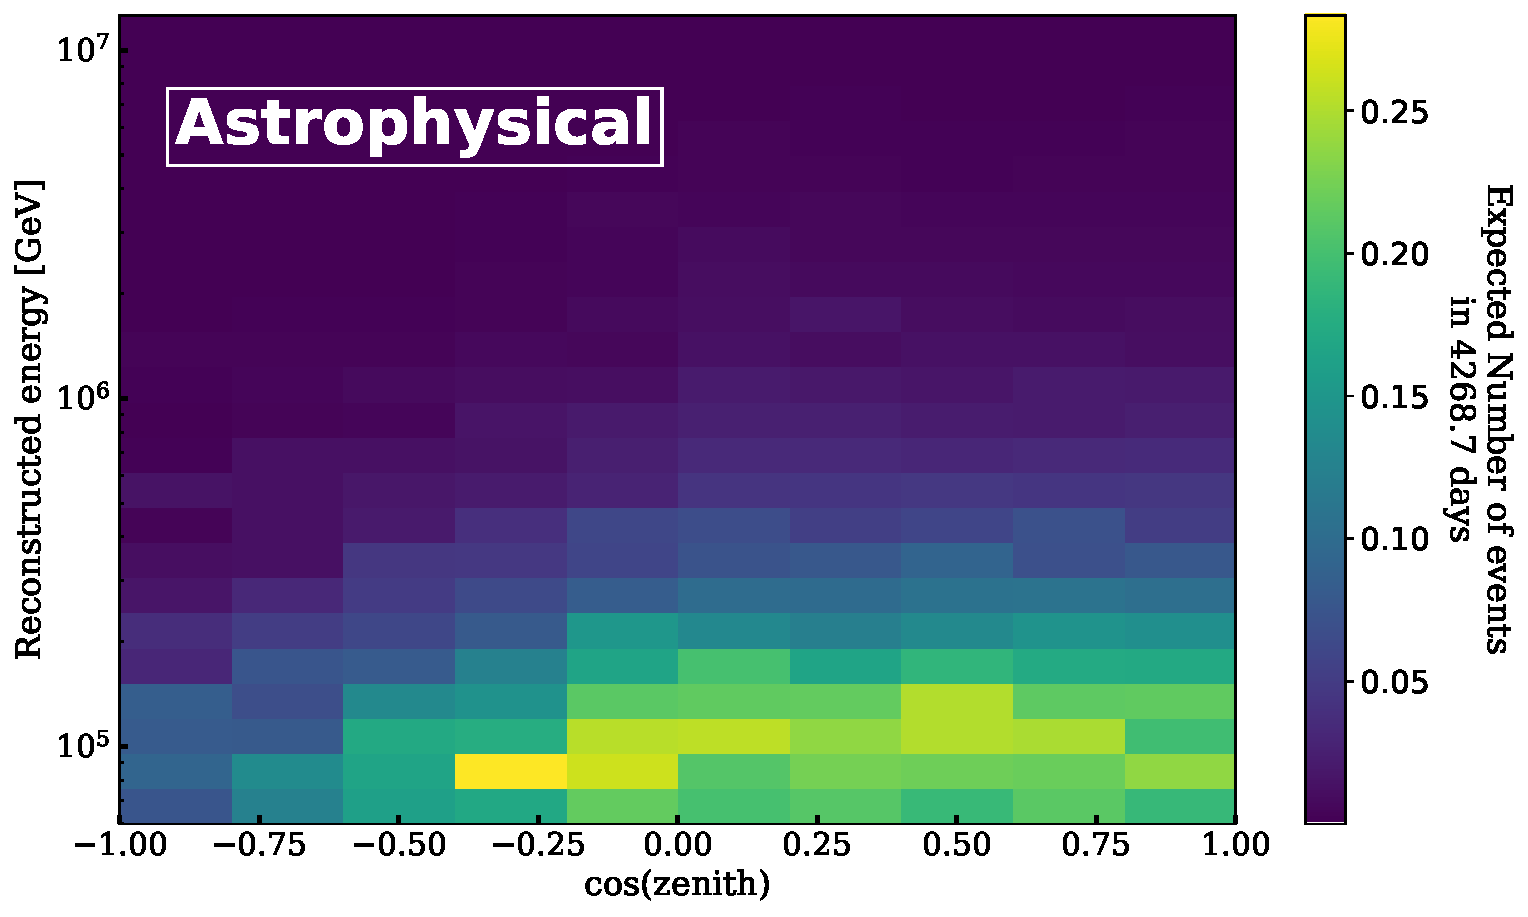
\includegraphics{./figures/Analysis/Tracks_Astrophysical.pdf}
    \end{subfigure}
    \hfill
    \begin{subfigure}[h]{0.72\textwidth}
        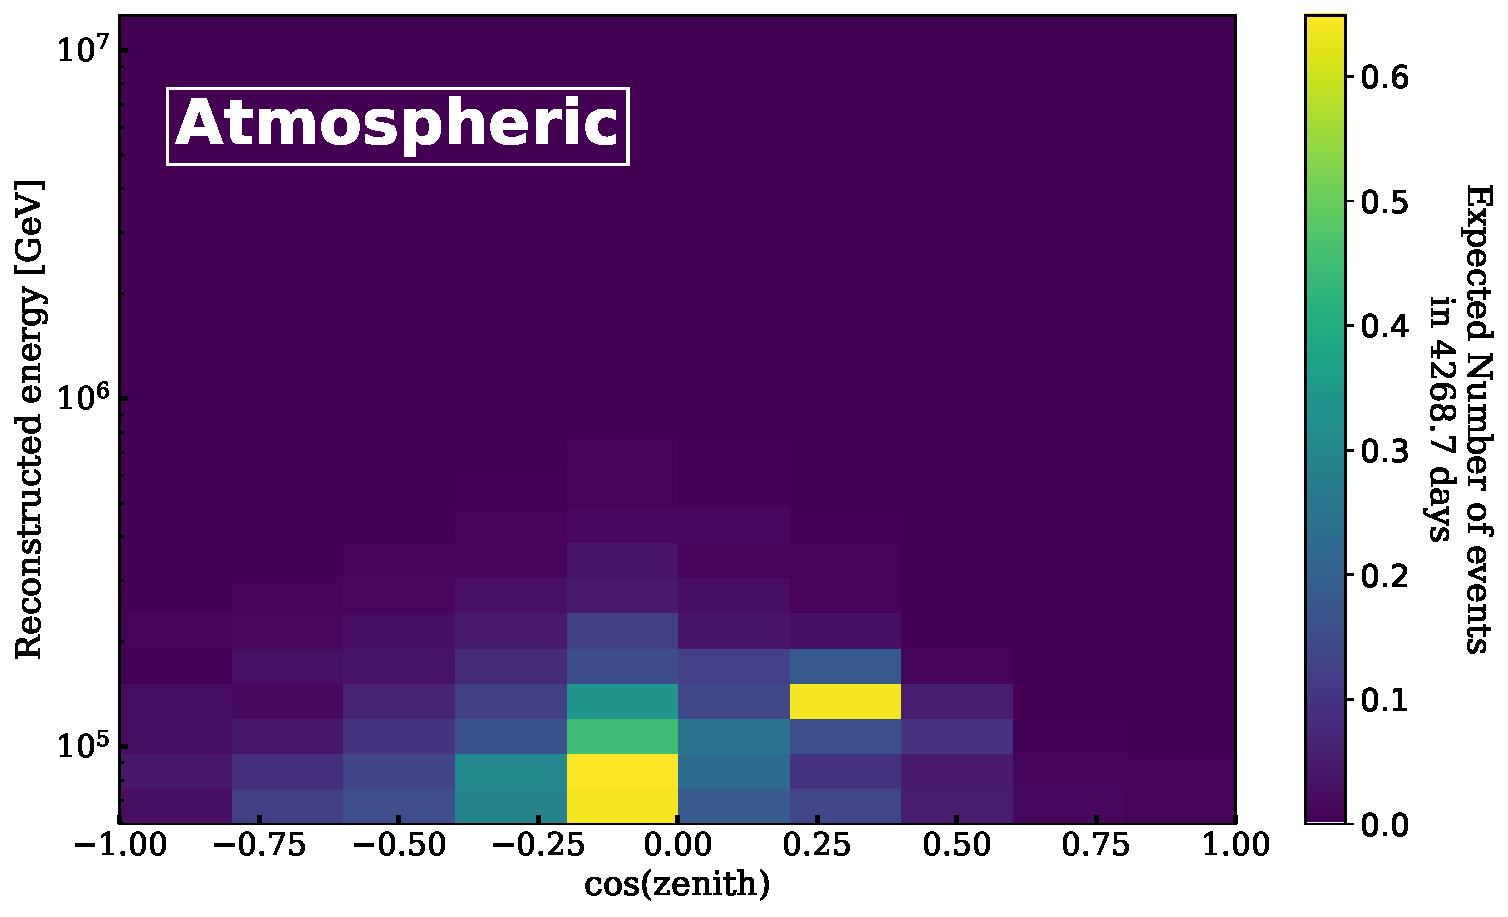
\includegraphics{./figures/Analysis/Tracks_Atmospheric.pdf}
       
    \end{subfigure}%
    \caption[2D Monte Carlo templates for tracks sample for astrophysical and atmopsheric fluxes]{2D Monte Carlo templates, constructed using reconstructed total energy ($E_{\text{Tot}}$) and reconstructed zenith ($\cos(\theta_z)$) for events classified as \textbf{tracks}. The signal (left), representing \emph{Astrophysical neutrinos} of the sample and the background (right), representing \emph{Atmospheric neutrinos}, including conventional, prompt and single muon fluxes.}
    \labfig{tracks_2d}
\end{figure*}

This becomes more evident in the one-dimensional (energy-averaged) distribution for both of these subsamples (\reffig{cascade_mc} for cascades and \reffig{tracks_mc} for tracks), where total expectation is broken down in individual flux contributions (as described in \ref{sec:params}). In the case of Energy distribution of single cascades (right panel of \reffig{cascade_mc}), except for lower energy bins (up to $\sim110$ TeV), astrophysical single cascade events dominate. The Glashow peak due to the resonant interaction of $\bar{\nu}_e$ is clearly visible too. Note the missing muon component, due to lack of enough \texttt{MUONGUN} simulation, as described in \ref{sec:params}. For Tracks (\reffig{tracks_mc}), there is a similar supression due to the self-veto effect. The constribution of single muons, simulated using \texttt{MUONGUN} events, is clearly visible, dominating in the same down-going region. As described before, the template is noisy due to large Monte Carlo uncertainties. In general, the tracks sample shows a larger contribution due to atmospheric fluxes compared to single cascades\sidenote{recall that single cascades also show contributions from all flavour Neutral Current (NC) interactions}. Similar one dimensional distributions of $\mathrm{L}_{\mathrm{dc}}$ and $\mathrm{E}_{\mathrm{Tot}}$ are shown for completeness in \reffig{double_mc}, but as described before, double cascades do not show any striking contributions from going the atmopsheric fluxes as the background for this sample is due to $\nu_{e}$ and $\nu_{\mu}$ events.


\begin{figure*}[h!]
    \caption[1D observable distribution of the total deposited energy and zenith angle for single cascades]{One-dimensional observable distribution, for HESE Single Cascades showing expected number of events as a function of reconstructed energy (right) and reconstructed zenith (left), broken down into different flux components, Astrophysical and Conventional Neutrinos and Muon (single muons). Only statistical errors of the MC simulation are shown.}
    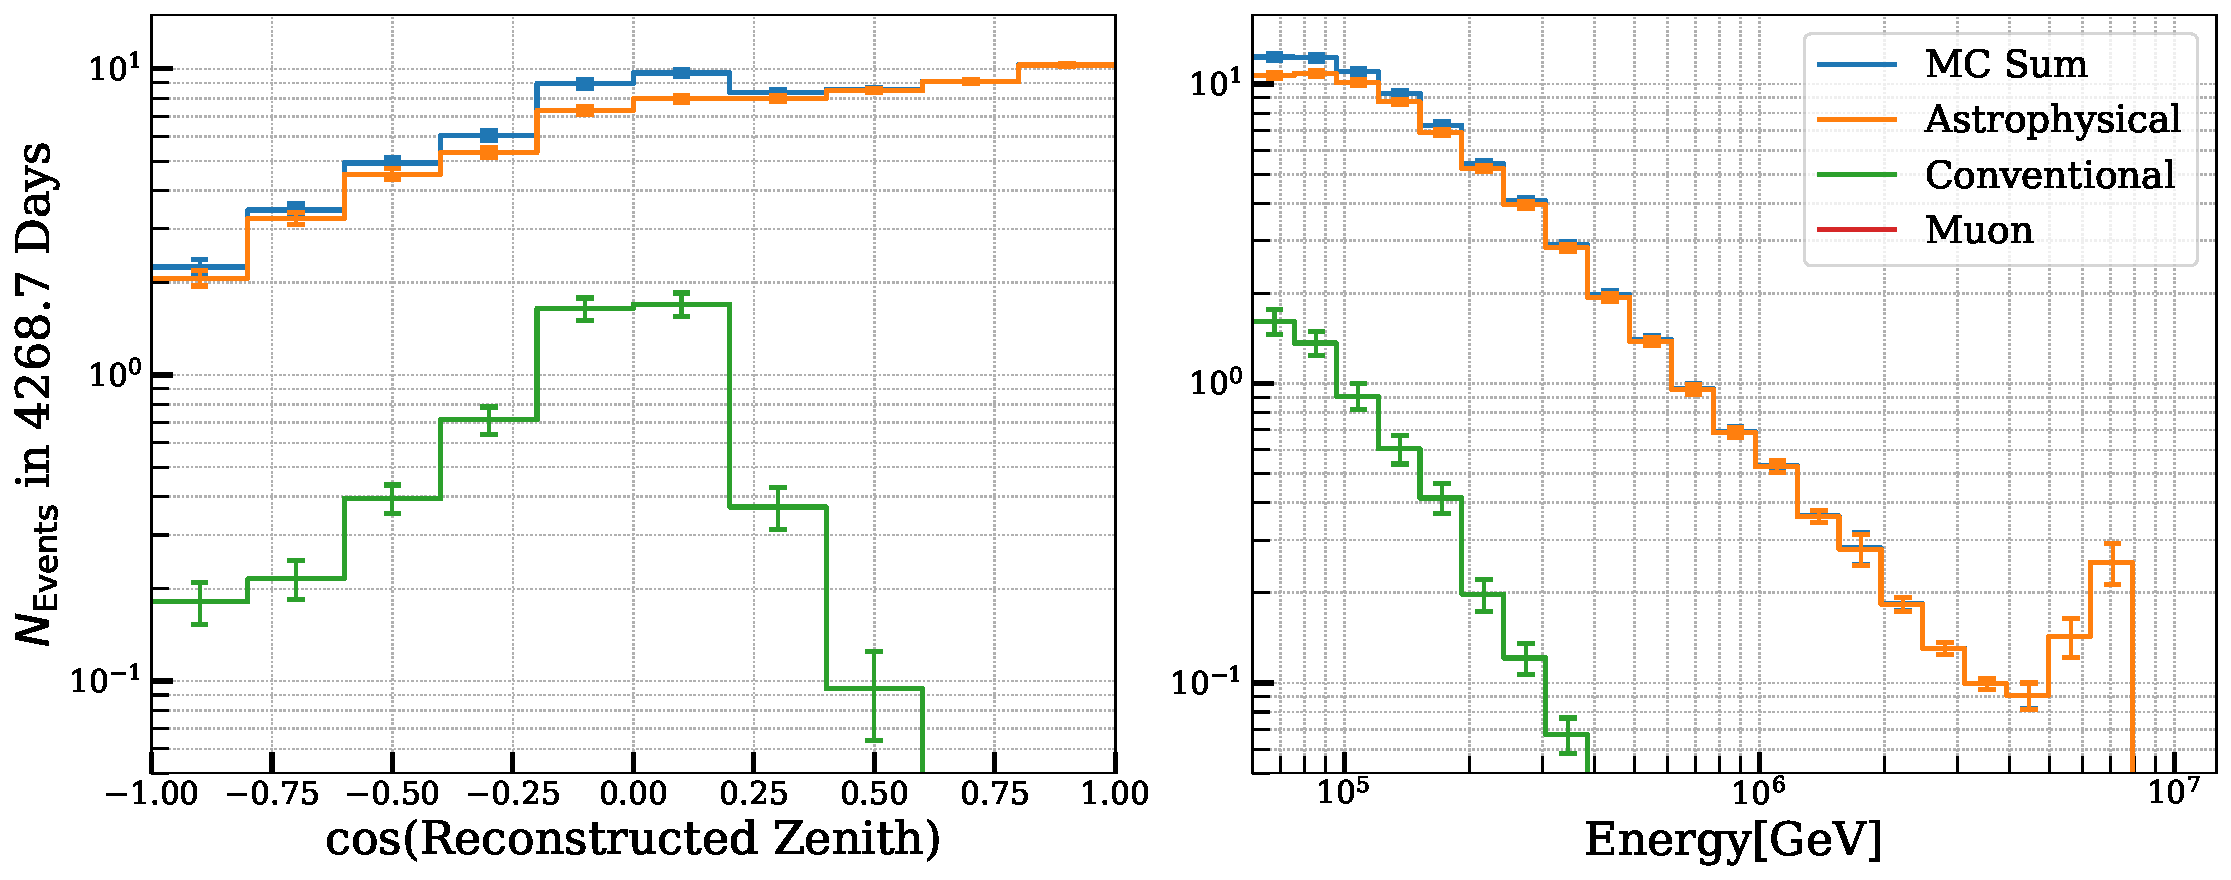
\includegraphics{./figures/Analysis/Cascades.pdf}
    \labfig{cascade_mc}
\end{figure*}

\begin{figure*}[h!]
    \caption[1D observable distribution of the total deposited energy and zenith angle for tracks]{One-dimensional observable distribution, for HESE Tracks showing expected number of events as a function of reconstructed energy (right) and reconstructed zenith (left), broken down into different flux components, Astrophysical and Conventional Neutrinos and Muon (single muons). Only statistical errors of the MC simulation are shown.}
    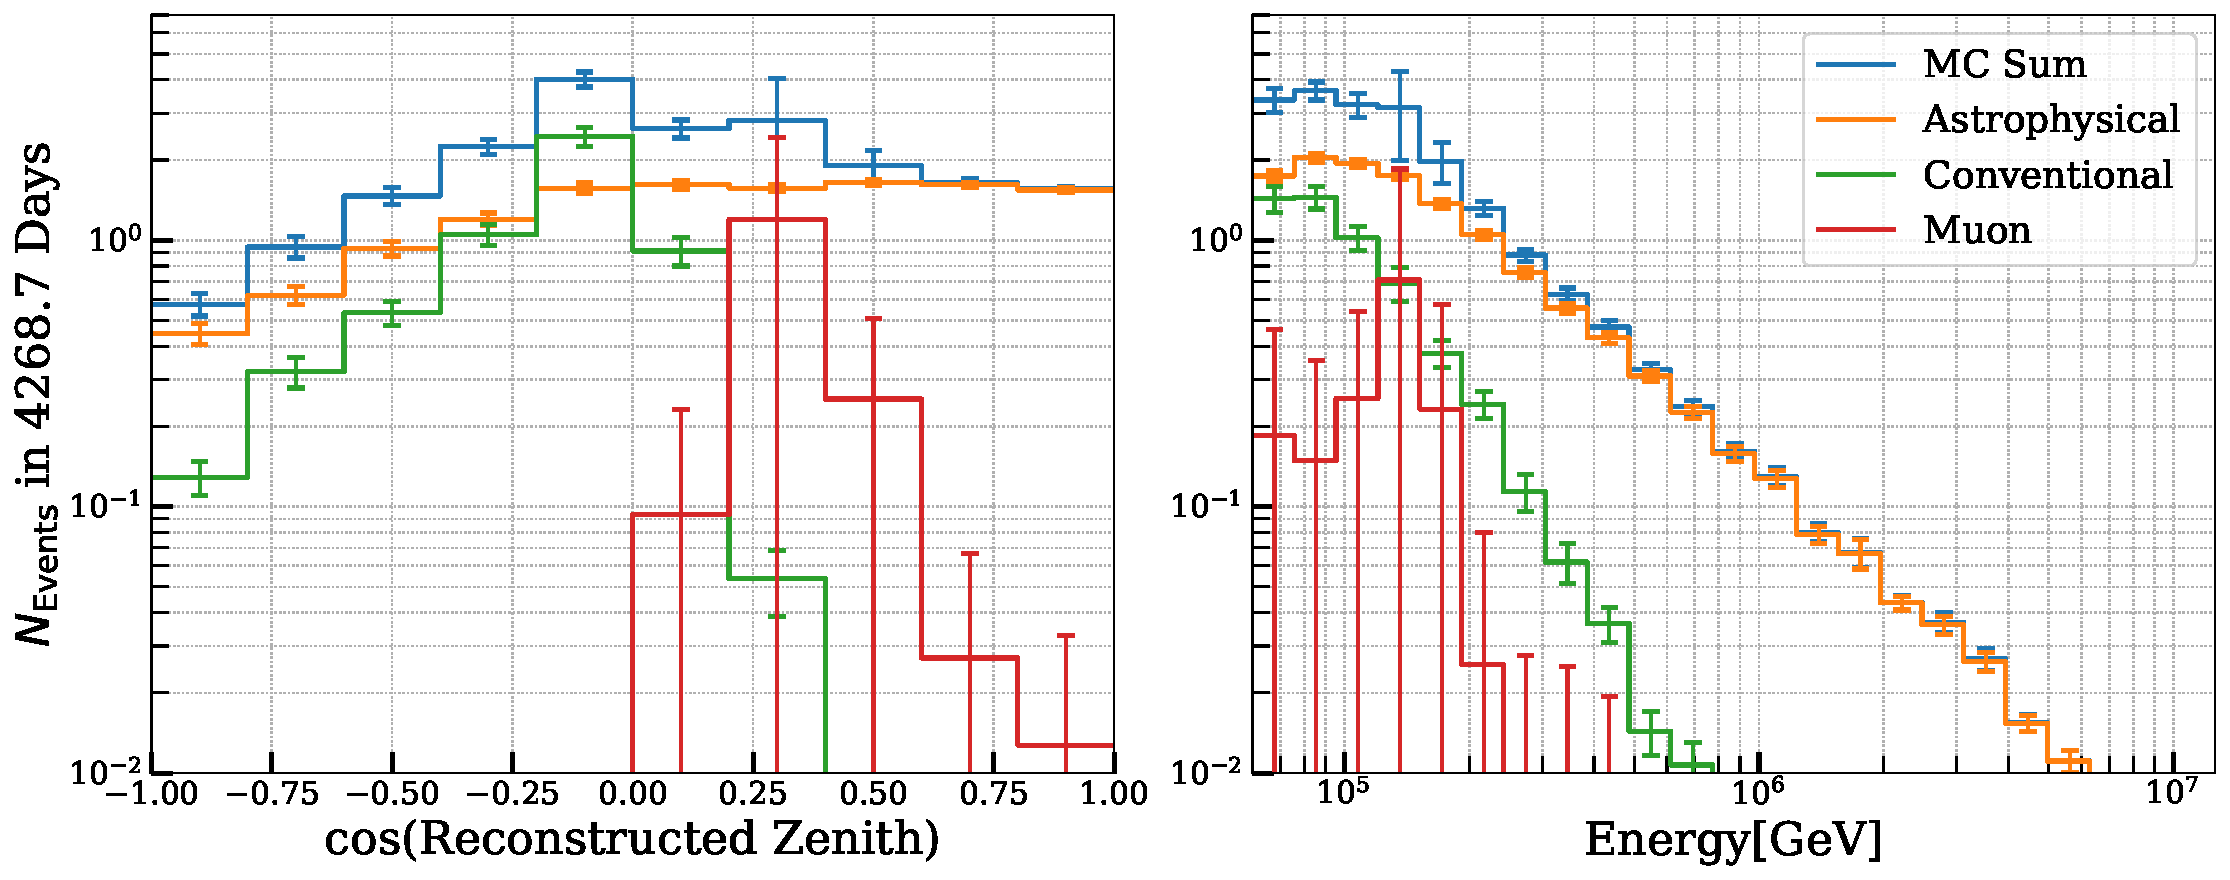
\includegraphics{./figures/Analysis/Tracks.pdf}
    \labfig{tracks_mc}
\end{figure*}

\begin{figure*}[h!]
    \caption[1D observable distribution of the total deposited energy and reconstructed tau decay length for double cascades]{One-dimensional observable distribution, for HESE Double Cascades showing expected number of events as a function of reconstructed energy (right) and reconstructed tau decay length (left), broken down into different flux components, Astrophysical and Conventional Neutrinos and Muon (single muons). Only statistical errors of the MC simulation are shown.}
    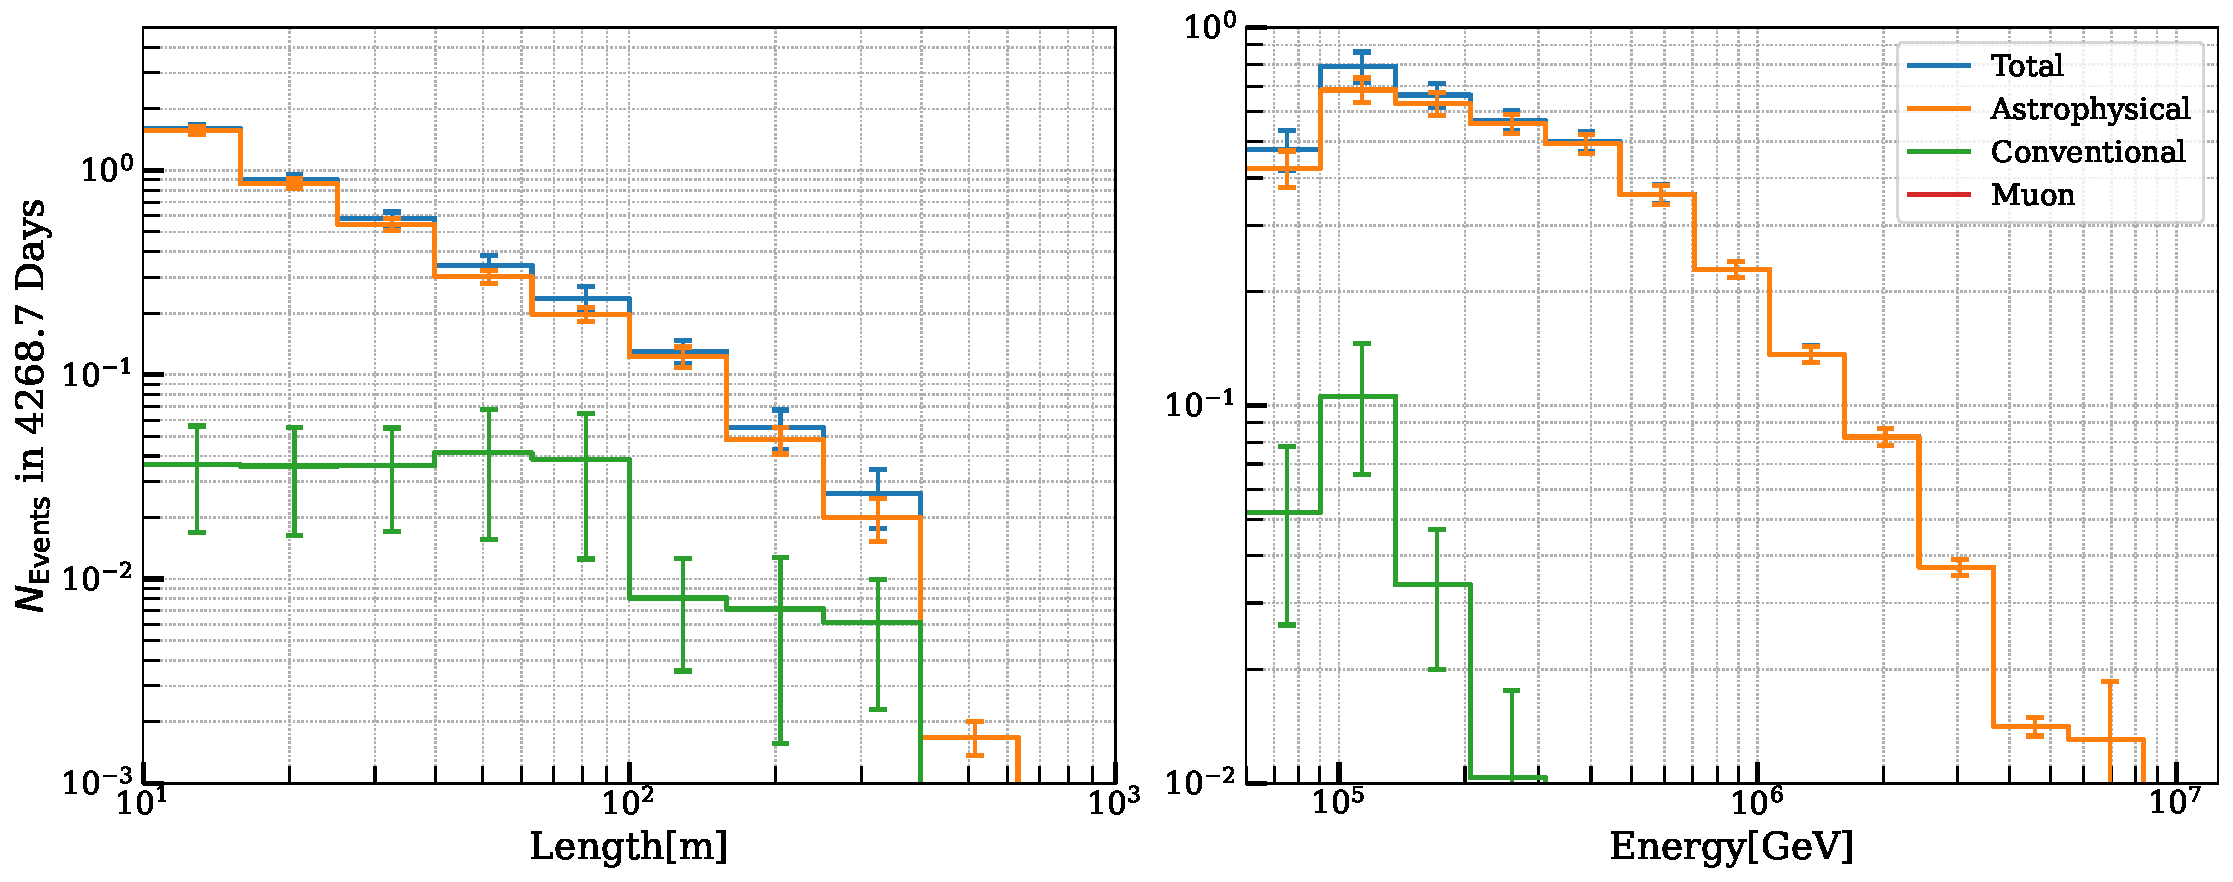
\includegraphics{./figures/Analysis/Double.pdf}
    \labfig{double_mc}
\end{figure*}

\section{Analysis Sensitivity}
\label{sec:sensitivty}
All fits and related calculations are carried out using a software toolkit called \textbf{\texttt{NNMFit}}. Developed within the IceCube collaboration, \texttt{NNMFit} has been applied in many other IceCube analyses. Essentially, the toolkit handles the statistical modeling required for forward-folding fits using high-energy neutrino data with binned likelihoods. It supports Monte Carlo event weighting, testing various flux models using signal and nuisance parameters, applying systematic detector uncertainties, and performing fits to data. The toolkit also enables joint fitting across different event selections. The \texttt{aesara} backend \sidecite{aesera} allows fast and efficient forward folding of Monte Carlo samples, even for large datasets, and offers automated differentiation that greatly assists in optimizing likelihood with gradient-aware minimizers \sidecite{LBFGSB}. More details on this toolkit can be found in \sidecite{richard_thesis,erik_thesis}. 

Using all the ingredients constructed from signal and nuisance parameters, and following the described method, the flavour composition parameter space is scanned to obtain a two-dimensional confidence region for the flavour composition, as shown in \reffig{sensitivity}. To derive these limits, an Asimov dataset is constructed (see Section~\ref{sec:analysis}), assuming the benchmark astrophysical neutrino spectrum given in Equation~\ref{eq:SPL}. All other nuisance parameters are assumed to be at their baseline values listed in \reftab{fit_params}. The astrophysical neutrino flavour composition is constrained by evaluating the likelihood ratio in a profile likelihood scan, with confidence regions estimated using Wilks’s theorem. The expected number of events over 12 years of HESE data, assuming the spectrum in \ref{eq:SPL}, is broken down by flux components and shown in \reftab{expected_events}. The fitting procedure bins all HESE events above 60 TeV in reconstructed energy and further categorizes them into three subsamples based on morphology: single cascades, tracks, and double cascades. The three samples are fit jointly using the respective two-dimensional Monte Carlo templates, with the appropriate analysis variables shown in \reffig{cascades_2d}, \reffig{tracks_2d}, and \reffig{LvsE_signalbkg}.

\begin{table}[h]
    \caption[The expected number of events in 12 years of HESE data]{The expected number of events from different flux components in the HESE sample, assuming a livetime of $\sim 12$ years, for single cascades, double cascades, and tracks categories. Only Monte Carlo uncertainties are included. The astrophysical spectrum assumed follows Equation~\ref{eq:SPL}.}
    \labtab{fit_params}
    
    \begin{tabular}{ c |c|c|c}
        
        \hline
        &Single Cascades &Double Cascades&Tracks\\
        \hline
        \hline
        Astrophysical&$67\pm1$& $4\pm0.2$ & $13\pm0.5$\\
        Conventional & $5\pm0.7$& $0.2\pm0.1$ &$5\pm0.6$\\
        Atm. Muons & - & - & $2\pm3$\\
        \hline
        MC Sum & $72\pm2$ & $4\pm0.3$ & $20\pm3$\\
        \hline
    \end{tabular}
\end{table}

\begin{figure}[h!]
    \caption[Sensitivity to the astrophysical neutrino flavour composiition using 12 years of HESE data]{Sensitivity of the analysis presented in this thesis to measure the the flavour composition using $\sim12$ years of IceCube HESE data. A single power law given in Equation~\ref{eq:SPL} is assumed, with flavour composition of $\nu_e:\nu_{\mu}:\nu_{\tau}=1:1:1$. Contours show the $1\sigma$ (solid) and $2\sigma$ (dashed) confidence intervals assuming Wilks' theorem.}
    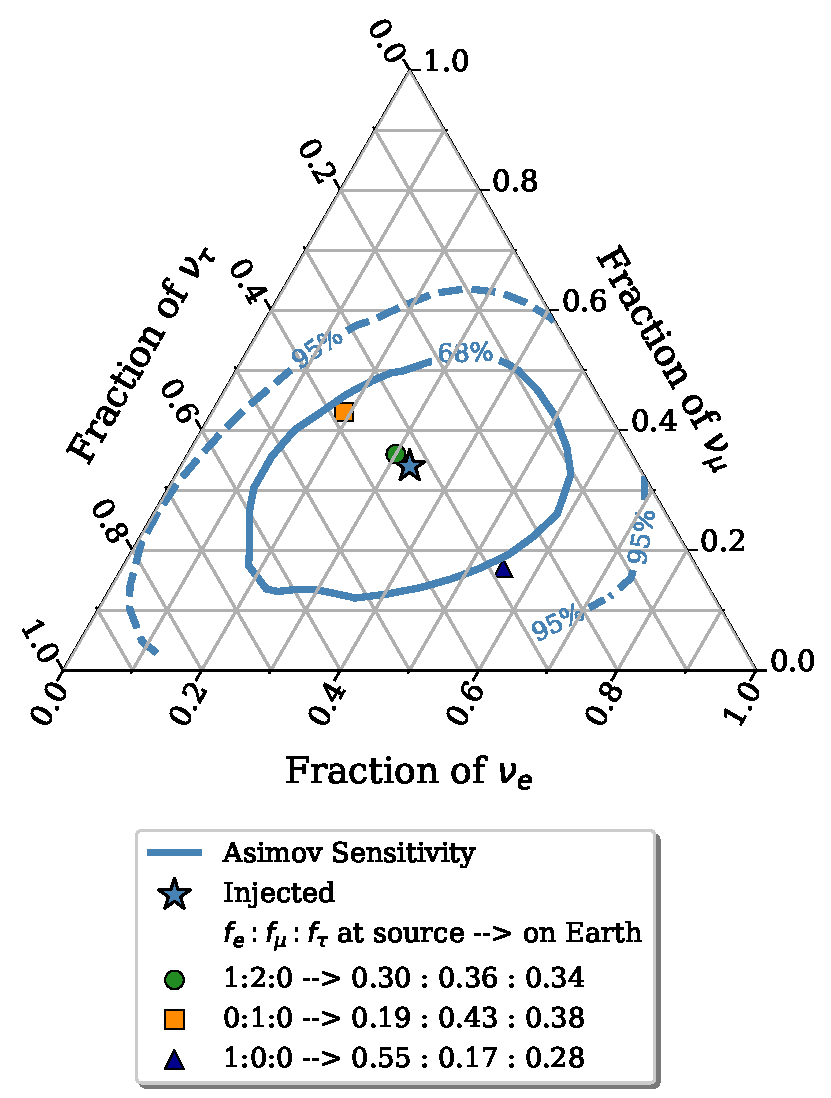
\includegraphics{./figures/Analysis/Asimov_Sensitivity.pdf}
    \labfig{sensitivity}
\end{figure}

The sensitivity results in \reffig{sensitivity} reveal that none of the standard source scenarios discussed in Section~\ref{sec:flavour_theory} can be rejected with high significance. For instance, the neutron beam scenario (represented by the dark blue triangle) is barely excluded at the $\sim1\sigma$ level. It is important to recall that the sensitivity of this analysis to the astrophysical tau-neutrino flux depends strongly on the assumed spectral shape of the neutrino flux. This sensitivity arises from the energy-dependent identification efficiency of tau-neutrino interactions. In interactions at higher neutrino energies, more energy is transferred to the secondary tau, increasing its decay length and enhancing identification efficiency. A softer spectrum, however, leads to more tau-neutrino interactions at lower energies, where they are harder to identify. Additionally, the sudden disappearance of line segments in the 95\% confidence contours, particularly in regions where the $\nu_\mu$ fraction approaches zero, is a result of the flavour fit parameterization (see Equation \ref{eq:flav_frac}). By construction, this fraction cannot be zero, meaning that this phase space is inaccessible to the fit\footnote{The \texttt{NNMFit} toolkit used in this analysis was initially developed for a spectrum measurement utilizing a sample of through-going tracks \cite{diffusenumu}. This sample, primarily consisting of muon neutrinos, was specifically designed to measure a non-zero \(\nu_{\mu}\) fraction, which informed the choice of flavour fraction parameterization. It is important to note, however, that alternative parameterization methods exist, where the flavour fractions of the three neutrino types are represented as a vector in three-dimensional space, with their relationships defined through a spherical coordinate transformation \cite{golemflavor}. This approach could also be implemented in \texttt{NNMFit}.}.

While earlier versions of this analysis explored alternative flux models (for example, a broken power law introduces a break in the conventional single power law, resulting in different spectral indices on either side of the break energy), this was not done here. The decision was based on recent findings from another IceCube analysis that combined two other event samples (track and cascade events, including much lower energies compared to HESE sample), revealing features in the extragalactic astrophysical neutrino spectrum based on the sensitivity to a larger range of astrophysical neutrino energies ($\sim10$ TeV to $\sim10$ PeV) \sidecite{globalfit_icrc}. That study provided evidence of a spectral break at around 24 TeV with more than $4\sigma$ significance. The spectrum showed hardness below this break, followed by softening at higher energies, consistent with the softer spectral measurement from HESE-7.5, which is sensitive to the astrophysical neutrino flux above $\sim 70$ TeV \sidecite{HESE7_sample}. Importantly, this high-statistics analysis, which extends well beyond the energy range of the current analysis, found no significant structures in the energy range accessible with the HESE sample. Furthermore, an independent study using a different event sample \sidecite{MESE_ICRC} reported similar spectral features and closely aligned best-fit values, strengthening the argument and above choice. 


\setchapterpreamble[u]{\margintoc}
\chapter{Results}
\labch{HESE12}
The 7.5 years of HESE data (2010-2017) was previously used to measure the composition of astrophysical neutrino flavors \sidecite{Juliana_paper} (in particular to search for $\nu_{\tau}$ events) and energy spectrum \sidecite{HESE7_sample}. This dataset included 102 events, (of which 60 events were above 60 TeV), that passed the HESE selection criteria, as outlined in section \ref{sec:HESE}. Two events were identified as Double Cascade candidates using the particle identifier described in section \ref{sec:PID}. 

For this iteration, the analysis has undergone significant changes compared to previous versions while maintaining consistent selection criteria and particle identification methods. The most notable difference lies in the ice model, specifically its properties and influence on the reconstruction of tau decay length, detailed in section \ref{sec:icemodel}. The SPICE-Bfr may have impacts on the overall energy estimates, as the number of photons collected in a given time window have significantly changed in this model of ice depending on the alignment of DOMs with respect to the iceflow axis \sidecite{BFR_paper}. Furthermore, the treatment of detector systematics has evolved, utilizing the SnowStorm method (see section \ref{sec:snowstorm}) instead of discrete Monte Carlo simulation sets used previously. The update also includes revised reconstruction tables \sidecite{updated_recotables_tianlu} for the maximum likelihood reconstruction method described in section \ref{sec:reco}. Additionally, various corrections have been applied to monte carlo simulations, encompassing reweighting to incorporate corrections due to tau polarization and initial state radiation corrections to the Glashow cross-sections (see section \ref{sec:PID}). Lastly, some of the nuisance parameters and analysis software are also different (see section \ref{sec:components}). As a first step, the 7.5 years of HESE data were re-unblinded due to these changes.

This chapter presents flavor measurements made using ~12 years (11.69 to be exact) of HESE data. It begins by discussing the re-unblinding of 7.5 years of data, followed by results from the 12-year fit, including Data-Monte Carlo agreement and detailed post-unblinding checks. Finally, the flavor measurement results are presented and interpreted in the last sectinons.

\section{(Re)Unblinding of 7.5 years of HESE Data}
\label{sec:HESE7}
The re-unblinding of the HESE-7.5 data provided new insights, revealing that 64 events met the HESE selection criteria, each with a deposited energy exceeding 60 TeV. It included 6 Double Cascade events\footnote{Unless explicitly specified, all mentioned classifications are by using SPICEBfr, the default icemodel of the analysis presented in this thesis. At some places in this section, specific comparisons are shown using SPICE-3.2.1}, which is a significant increase from the previous analysis that identified only two Double Cascade events. Notably, 4 of the additional events had initially been classified as single cascades. The reclassification was largely driven by the application of the energy asymmetry cut, which proved to be a crucial factor in differentiating between single and double cascades (see section \ref{sec:PID}). A key difference in this re-unblinding was the icemodel used for reconstruction, as mentioned before. Hence, the data was processed using both SPICE-3.2.1 (used in previous iteration) and SPICE-Bfr to make direct comparisons with the previous results. Using SPICE-3.2.1, reunblinded data contained total of 62 HESE events above 60 TeV deposited energy, of which 7 events were classified as Double Cascades. Moreover, of these 6 and 7 observed Double Cascades, using different ice models, only 3 are common, landing 7 new candidate events. Despite the changes in the total number of classified events, the two common Double Cascade events identified in both iterations exhibited nearly identical reconstructed properties, as outlined in \reftab{reco_values_comparisons_spice} (for SPICE-3.2.1). \todo{should there be a similar table for bfr??} %and \reftab{reco_values_comparisons_bfr} (for SPICEBfr)   


% \begin{table*}[h!]
%     \caption{Comparison of Reconstructed quantities of events classified as Double Cascades upon re-unbling 7.5 years of HESE data  using \textbf{SPICEBfr icemodel} with previous results (grey cells). Shown in the table are (from left), MJD (Modified Julian Date), reconstructed length, reconstructed Energy of first ($\mathrm{E}_1$) and second ($\mathrm{E}_2$) cascades, Energy asymmetry ($\mathrm{E}_\mathrm{A}$), Energy Confinement ($\mathrm{E}_\mathrm{C}$) and classified morphology of the event. The two common events, 57134 (\emph{Double Double}) and 56265 (\emph{Big Bird}) have nearly identical reconstructed quantities.}
%     \labtab{reco_values_comparisons_bfr}
%     \begin{tabular}{c|cc|cc|cc|cc|cc|cc}
%         \toprule
%          MJD    & \multicolumn{2}{c|}{Length}
                
%                         & \multicolumn{2}{c|}{$\mathrm{E}_\mathrm{1}$}
%                                 & \multicolumn{2}{c|}{$\mathrm{E}_\mathrm{2}$} 
%                                     & \multicolumn{2}{c|}{$\mathrm{E}_\mathrm{A}$} 
%                                         & \multicolumn{2}{c|}{$\mathrm{E}_\mathrm{C}$}  
%                                             & \multicolumn{2}{c}{morphology}                \\
                       
%         \midrule
%         57835   &   13 m   & \cellcolor{lightgray}66 m    & 19 TeV   &   \cellcolor{lightgray}79 TeV  &   73 TeV  &   \cellcolor{lightgray}3 TeV  &   -0.58  &   \cellcolor{lightgray}0.93 & 1 &  \cellcolor{lightgray}1&Double& \cellcolor{lightgray}Single\\
%             % \hline
%         57134   &   17 m   & \cellcolor{lightgray}17 m    & 5.7 TeV   &   \cellcolor{lightgray}8.7 TeV  &   92 TeV  &   \cellcolor{lightgray}79 TeV  &   -0.89  &   \cellcolor{lightgray}-0.80 & 0.99 &  \cellcolor{lightgray}0.99&Double& \cellcolor{lightgray}Double\\
%             % \hline
%         56603   & 13 m   & \cellcolor{lightgray}70 m    & 32 TeV   &   \cellcolor{lightgray}85 TeV  &    48 TeV  &   \cellcolor{lightgray}1 TeV  &   -0.19  &   \cellcolor{lightgray}1 & 1 &  \cellcolor{lightgray}0.99 & Double & \cellcolor{lightgray}Single\\
%             % \hline
%         55714   &   14 m   & \cellcolor{lightgray}26 m    & 5 TeV   &   \cellcolor{lightgray}58 TeV  &   82 TeV  &   \cellcolor{lightgray}16 TeV  &   -0.88  &   \cellcolor{lightgray}0.55 & 0.99 &  \cellcolor{lightgray}1&Double& \cellcolor{lightgray}Single\\
%             % \hline
%         55800   &   13 m   & \cellcolor{lightgray}20 m    & 128 TeV   &   \cellcolor{lightgray}133 TeV  &   72 TeV  &   \cellcolor{lightgray}38 TeV  &   0.28  &   \cellcolor{lightgray}0.55 & 1 &  \cellcolor{lightgray}0.99&Double& \cellcolor{lightgray}Single\\
%             % \hline
%         56265   &  16 m   & \cellcolor{lightgray}16 m    & 1.1 PeV   &   \cellcolor{lightgray}1.2 PeV  &   0.9 PeV  &   \cellcolor{lightgray}0.6 PeV  &   0.09  &   \cellcolor{lightgray}0.29 & 1 &  \cellcolor{lightgray}1&Double& \cellcolor{lightgray}Double\\
%             \bottomrule
%     \end{tabular}
% \end{table*}

\begin{table*}[h!]
    \caption{Comparison of Reconstructed quantities of events classified as Double Cascades upon re-unbling 7.5 years of HESE data using \textbf{SPICE-3.2.1 icemodel} with previous results (grey cells). Shown in the table are (from left), MJD (Modified Julian Date), reconstructed length, reconstructed Energy of first ($\mathrm{E}_1$) and second ($\mathrm{E}_2$) cascades, Energy asymmetry ($\mathrm{E}_\mathrm{A}$), Energy Confinement ($\mathrm{E}_\mathrm{C}$) and classified morphology (as per previous anlaysis) of the event. The two common events, 57134 (\emph{Double Double}) and 56265 (\emph{Big Bird}) have nearly identical reconstructed quantities. The most striking differences here are specifically reconstructed length and the fact that $\mathrm{E}_1$ and $\mathrm{E}_2$ seem to be almost flipped for some events, even though reconstructed directions (zenith and azimuth, not shown in the table) remains almost idnetical. The change in $\mathrm{E}_1$ and $\mathrm{E}_2$ changes the $\mathrm{E}_\mathrm{A}$, which is the discrimation cut between single and double cascades.}
    \labtab{reco_values_comparisons_spice}
    \begin{tabular}{c|cc|cc|cc|cc|cc|c}
        \toprule
         MJD    & \multicolumn{2}{c|}{Length}
                
                        & \multicolumn{2}{c|}{$\mathrm{E}_\mathrm{1}$}
                                & \multicolumn{2}{c|}{$\mathrm{E}_\mathrm{2}$} 
                                    & \multicolumn{2}{c|}{$\mathrm{E}_\mathrm{A}$} 
                                        & \multicolumn{2}{c|}{$\mathrm{E}_\mathrm{C}$}  
                                            & \multicolumn{1}{c}{morphology}                \\
                       
        \midrule
        57677   &   27 m   & \cellcolor{lightgray}37 m    & 3.1 TeV   &   \cellcolor{lightgray}128 TeV  &   148 TeV  &   \cellcolor{lightgray}4 TeV  &   -0.96  &   \cellcolor{lightgray}0.94 & 1 &  \cellcolor{lightgray}0.99& \cellcolor{lightgray}Single\\
            % \hline
        57134   &   16 m   & \cellcolor{lightgray}17 m    & 18 TeV   &   \cellcolor{lightgray}8.7 TeV  &   92 TeV  &   \cellcolor{lightgray}79 TeV  &   -0.89  &   \cellcolor{lightgray}-0.80 & 0.99 &  \cellcolor{lightgray}0.99& \cellcolor{lightgray}Double\\
            % \hline
        56763   & 10.2 m   & \cellcolor{lightgray}84 m    & 63 TeV   &   \cellcolor{lightgray}107 TeV  &    87 TeV  &   \cellcolor{lightgray}17 TeV  &   -0.16  &   \cellcolor{lightgray}0.72 & 0.99 &  \cellcolor{lightgray}0.99  & \cellcolor{lightgray}Single\\
            % \hline
        55477   &   14 m   & \cellcolor{lightgray}279 m    & 70 TeV   &   \cellcolor{lightgray}184 TeV  &   84 TeV  &   \cellcolor{lightgray}67 TeV  &   -0.09  &   \cellcolor{lightgray}0.46 & 0.99 &  \cellcolor{lightgray}0.98& \cellcolor{lightgray}Single\\
            % \hline
        55800   &   12 m   & \cellcolor{lightgray}20 m    & 105 TeV   &   \cellcolor{lightgray}133 TeV  &   89 TeV  &   \cellcolor{lightgray}38 TeV  &   0.08  &   \cellcolor{lightgray}0.55 & 1 &  \cellcolor{lightgray}0.99& \cellcolor{lightgray}Single\\
            % \hline

        56221   &  12 m   & \cellcolor{lightgray}12 m    & 209 TeV   &   \cellcolor{lightgray}102 TeV  &   132 TeV  &   \cellcolor{lightgray}237 TeV  &   0.22  &   \cellcolor{lightgray}-0.4 & 0.99 &  \cellcolor{lightgray}0.97& \cellcolor{lightgray}Track\\
            
        56265   &  17 m   & \cellcolor{lightgray}16 m    & 0.8 PeV   &   \cellcolor{lightgray}1.2 PeV  &   1 PeV  &   \cellcolor{lightgray}0.6 PeV  &   -0.08  &   \cellcolor{lightgray}0.29 & 0.99 &  \cellcolor{lightgray}1& \cellcolor{lightgray}Double\\
            \bottomrule
    \end{tabular}
\end{table*}

No matter what icemodel is used, in reunblinding an excess of double cascade events was observed, suggesting the presence of unnoticed changes not already accounted for. Careful search of each step in the particle identification process revealed a significant change in the reconstruction method from the previous iteration. Notably, this change involved the incorporation of high quantum efficiency Digital Optical Modules (DOMs) from DeepCore. In earlier analyses, these DOMs had been excluded from the reconstruction of high-energy neutrino events, in millipede-based reconstructions outlined in \ref{sec:reco}. The rationale for their exclusion stemmed from the smaller statistical uncertainties of digitized waveforms, in compared to the systematic uncertainties. These systematic uncertainties, which were not well-characterized for individual DOMs, could not be factored into the table-based likelihood fitting method. Nonetheless, due to advancements in simulation, including enhanced reconstruction tables and detector simulations, the analysis presented in this thesis included the DeepCore DOMs, hence the next step was to explore why Monte Carlo predictions had underestimated the number of Double Cascade events. 

\begin{figure*}
    \begin{subfigure}[h]{0.7\textwidth}
        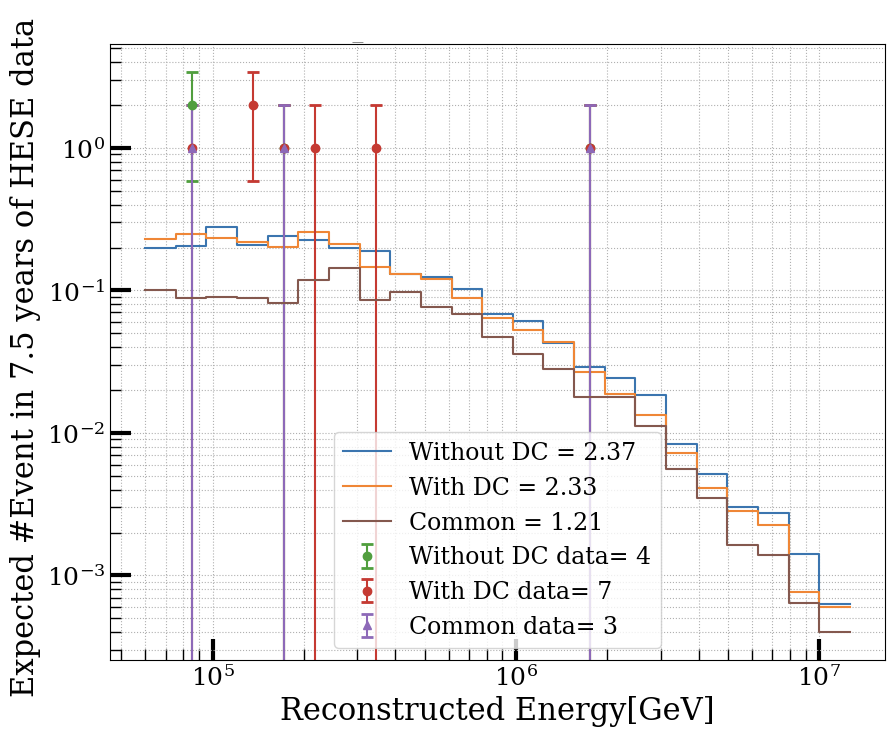
\includegraphics{./figures/results/Spice_DCwithdata.png}
    \end{subfigure}
    \hfill
    \begin{subfigure}[h]{0.7\textwidth}
        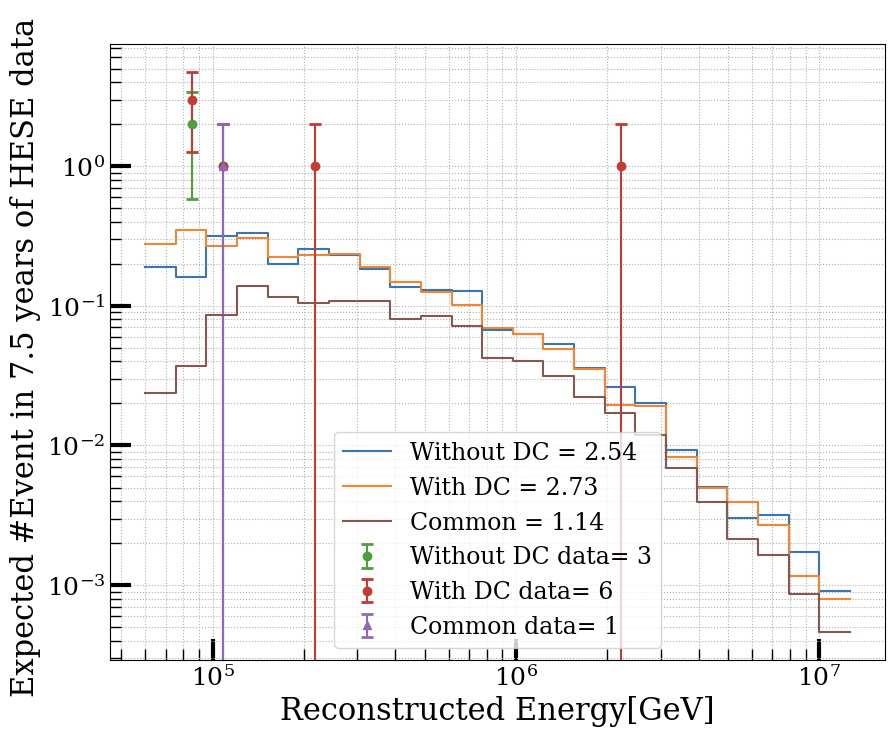
\includegraphics{./figures/results/Bfr_DCwithdata.png}
       
    \end{subfigure}%
    \caption{Distribution of number of expected classified as double cascacdes in 7.5 years of HESE data usign SPICE-3.2.1 (left) and SPICE-Bfr(right) icemodel with (\emph{With DC}) and without (\emph{Without DC}) DeepCore DOMs, along with data events for the respective configurations.}
    \labfig{Bfr_DCwithdata}
\end{figure*}

\reffig{Bfr_DCwithdata} shows the distribution of classified Double Cascade, both with and without the inclusion of DeepCore DOMs. The monte carlo simulations predicts only $\sim 2$ Double Cascade events, yet the data revealed 6 (7) Double Cascade events using SPICE-Bfr (SPICE-3.2.1) when DeepCore DOMs were included and only 3 (4) when they were excluded. It remains clear that no matter what icemodel is used, the distribution of reconstructed energy and overall expectation remains same irrespective of whether DeepCore DOMs are included or not. This discrepancy pointed to potential issues in either the simulation or reconstruction processes involving DeepCore DOMs\todo{In one of the appendix, a short discussion about SPE charge distribution checks done with jvs shall be included}, indicating that further investigation at the monte carlo level is necessary. Such investigations requires efforts that were beyond the timeline of this thesis work and  considering the historical exclusion of DeepCore DOMs (as well as other "bad" DOMs like bright or saturated modules) from reconstruction chains in previous iterations of HESE analyses, this analysis ultimately decided not to include DeepCore DOMs in the full sample unblinding. Ultimately, the re-unblinding of the HESE-7.5 data resulted in 62 events with deposited energies above 60 TeV. Of these, 45 were classified as single cascades, 3 as Double Cascades, and 14 as track events. A detailed comparison between these  reunblinded results and previous results, including classified morphologies (with different iterations of icemodels and DeepCore inclusion/exclusion) is shown in \reftab{HESE7_eventcomparisons}.

\begin{table*}[h]
    \caption[Event classification of 7.5 years of HESE data]{Event classification of 7.5 years of HESE data (Previous) compared with reunblinded sample outcome (all events have Reconstructed total energy > 60 TeV ). The comparison is shown for all 2 different icemodels, each of which further broken down into with and without the deepcore doms. The final outcome of this reunblinding, in order to move forward with the full sample is the last column (without DeepCore using SPICEBfr).}
    \labtab{HESE7_eventcomparisons}
    \raggedright
    \begin{tabular}{ c|c|c c |cc}
        \toprule
            & & \multicolumn{4}{c}{Reunblinded}\\
            
           Morphology&Previous & \multicolumn{2}{c|}{SPICE-3.2.1} & \multicolumn{2}{c}{SPICE-Bfr}\\
           
                     &   & DeepCore & No DeepCore & DeepCore & No DeepCore\\
                                
        \hline
        Cascades & 41 & 41 & 44 &42&45 \\
        Double Cascades & 2 & 7 &4&6& 3 \\
        Tracks& 17&14&14&16&14\\
        \hline
        Total & 60 & 62 &62&64&62\\
        \bottomrule
\end{tabular}
\end{table*}


\section{Unblinding of 12 years of HESE data}
\label{sec:HESE12}
The High-Energy Starting Events (HESE) sample, covering approximately 12 years of IceCube detector live time (4268.7 days) from 2010 to August 2022, was unblinded in January 2024 for the analysis outlined in Section 4.3. This sample includes 167 events that passed the HESE selection criteria, which involved the veto and total charge conditions as detailed in Section 4.2. Of these, 3 were coincident events that had previously been removed by manual inspection, but were retained this time since the current Monte Carlo simulations now account for such coincidences. Despite this, the energy threshold of 60 TeV effectively filtered them out, resulting in a final sample of 97 events above the 60 TeV deposited energy threshold. Using the ternary topology identification method from this thesis, 64 events were classified as single cascades, 5 as double cascades, and 28 as tracks.



\subsection{Fit results}
\label{sec:HESE12_fitresults}

\subsubsection{Blind Fit results}
\label{blindfit}
In IceCube, all the analysis are done in a blind fashion, meaning reconstruction and other fit details are applied to simulation to produce expectations in form of Monte Carlo PDFs and later data is fit to this expectation to make the desired measurement. Details of such a fit are given in \ref{sec:analysis}. For such fits, before looking at the full data results, sometimes a middle step is considered where only nuisance parameters are revealed first (and/or only background region is looked at) to see any striking disagreement between the data and monte carlo or unexplainable behaviour of any nuisance parameters (e.g. if they are hitting the fit range boundary etc).  Stopping criterions are set-up beforehand in case this step shows any troublesome results. For HESE sample, since overall expectation is quite low, looking at a subsample would certainly be unyielding. Thus, blindfit for this analysis included observing the nuisance parameters behaviour and goodness of the fit. The stopping criterions included, minimum p-value of 5\% for the goodness of fit test (see \ref{sec:analysis} for details) and applying priors on systematics in case they hit the boundary. These priors are derived from the so far gathered best knowledge of the ice and detector, and were tested by running pseudo trials (see \ref{sec:hists}) to test their effects on signal distributions. As a post-unblinding check, they are to be removed to see if any significant changes are observed in signal parameters. 

The bestfir values of nuisance parameters are summarized in \reftab{bf_nuisance} along with their gaussian priors. Initially, the holeice parameters, $\eta_{\mathrm{h.ice-p0}}$ and $\eta_{\mathrm{h.ice-p1}}$ were hitting the boundary, but upon applying the tested priors this effect was resolved. As a post unblinding check, these priors were removed to check any changes in signal parameters, no such significant changes were observed. The likelihood includes a penalty term (see \ref{sec:analysis}) which was checked for the 2D scan of flavour ratio triangle to see the effect of pulls due to this prior. \todo{perhaps the triangle plot showing llh penalty due to these priors can be shown here? or should this discussion have its separate appendix?}    

\begin{figure}[ht]
	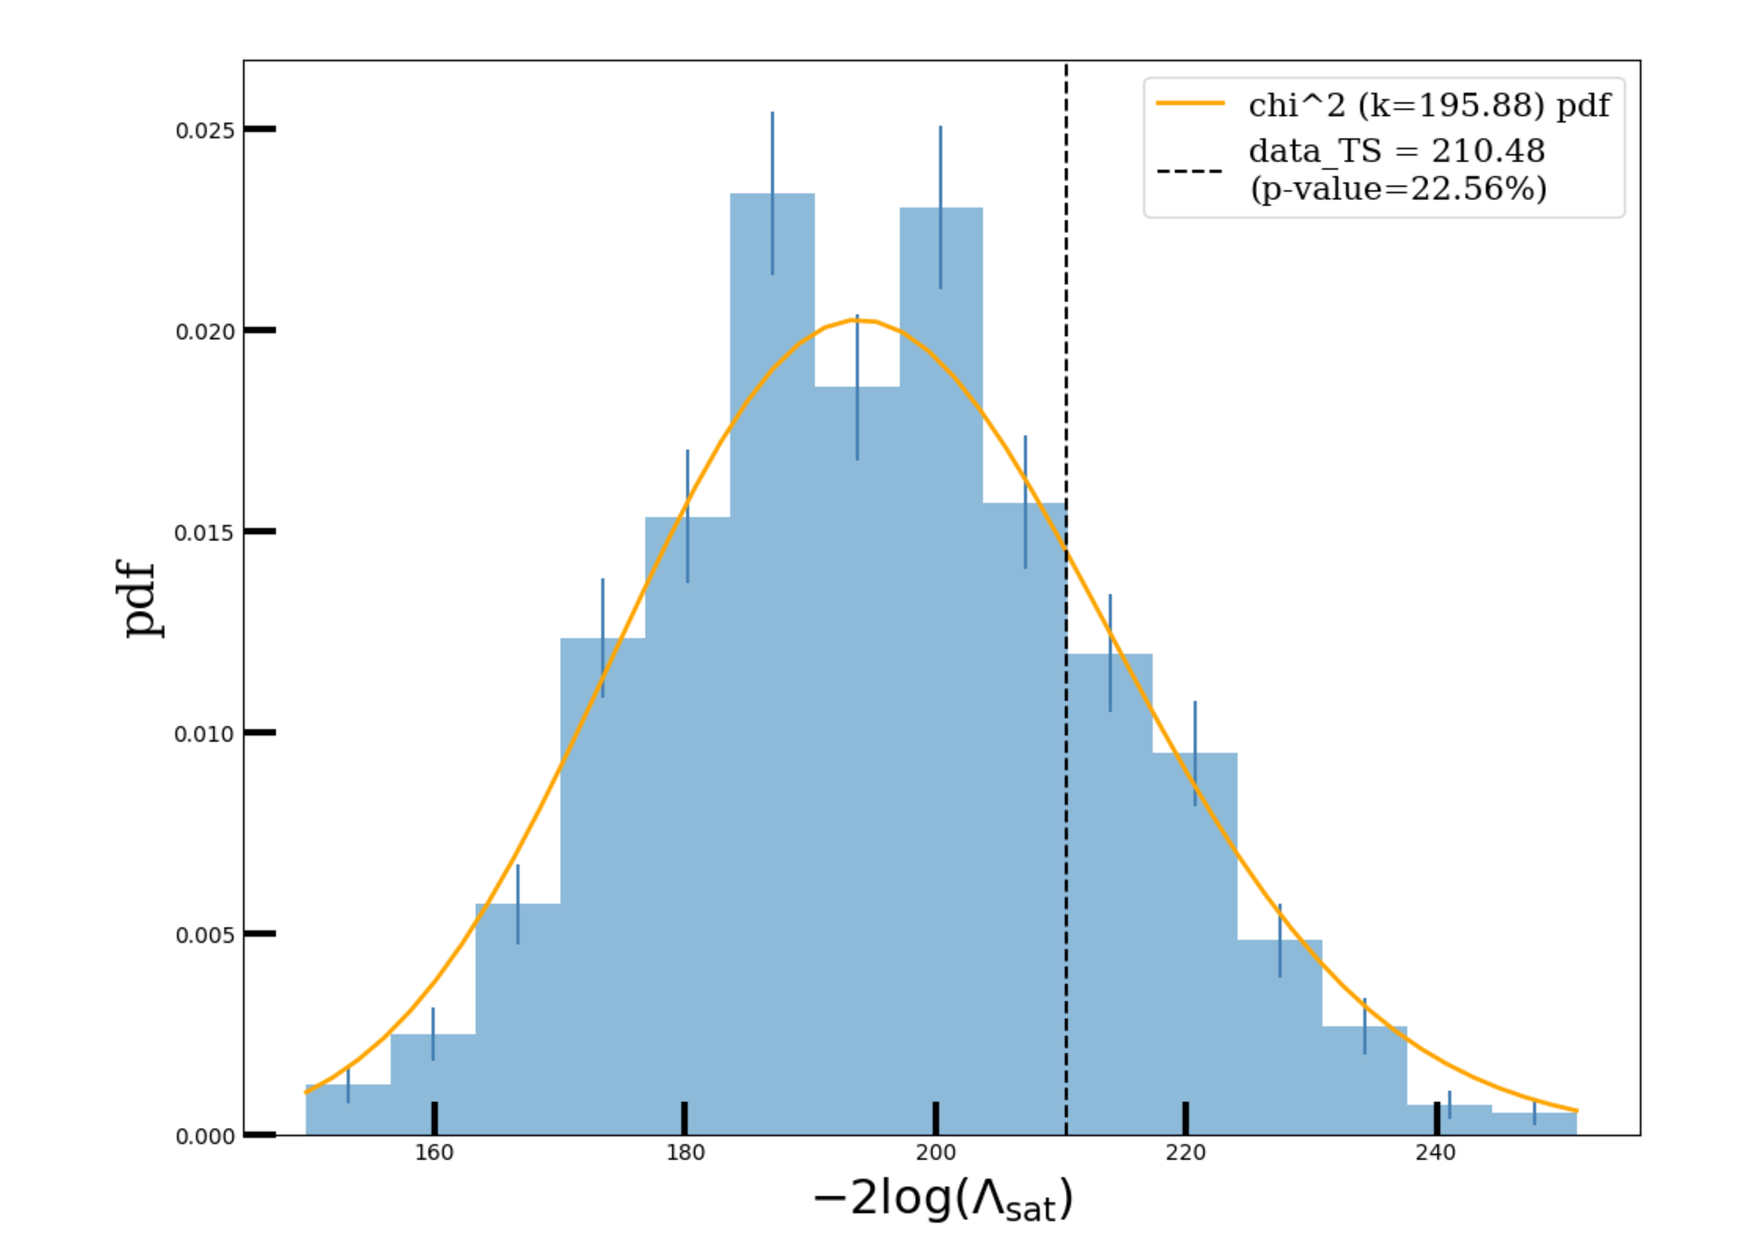
\includegraphics[scale=0.5]{./figures/results/GOF.pdf}
	\caption{Distribution of the test statistics for 1000 pseudotrials injected at bestfit (signal parameters kept blind). Veritcal line shows TS of data, which matches quite well with degrees of freedom derived by fitting a $\chi^2$ to the distribution.}
    \labfig{gof}
\end{figure}

Most of the nuisance parameters are primarily fitted to their priors with minimal deviations from the modeled uncertainties. The detector systematics are set away from default values, although they still remain within one standard deviation of the applied prior width. This can be explained as follows: The method used to apply systematic uncertainties, known as the "gradient method" (see \ref{sec:params}), in the fit assumes linearity whether moving away from or towards the central value. In an ideal scenario, the range within which the parameter is allowed to vary (and the simulation range) should be narrow enough that the central value can always be recovered. However, these parameters are considered only as nuisance in the fit, and they are not meant to be measured. Furthermore, the detector is not so precisely calibrated as to know the true value of these parameters. Therefore, in practice, the range is kept quite wide. In the analysis presented here, where the overall expectation is low and the data is binned in histograms, such things can happen, causing the nuisance parameters to shift.  In order to save computational power, the gradients are calculated once for a given spectrum assumption. If the underlying spectrum of data is far from this assumed spectrum, small changes in these signal parameters can cause larger deviations. Most of these systematics thus ended up having a gaussian prior in the fit, as listed in the \reftab{bf_nuisance}. 
 
\begin{table*}[h]
    \caption{The best-fit parameter values of the nuisance parameters. The uncertainties are calculated at the 68\% confidence level through a profile likelihood scan assuming Wilks' theorem, in case of a flat likelihood space, fit boundaries are given as limits. Last column states the gaussian priors on the parameters (if applicable) in terms of the mean ($\mu$) and width ($\sigma$). The table is divided in terms of type of the nuisance parameters, above part includes all the parameters that affects the atmosphgeric neutrino components and the lower part consists if parameters stemming through various detector components. For details, see \ref{sec:params}}
    \labtab{bf_nuisance}
    {\renewcommand{\arraystretch}{1.4}
    \begin{tabular}{ c c |c|c}
        \hline
        \multicolumn{2}{c|}{Parameter}  & Best-Fit value & Prior ($\mu,\sigma$)\\
        \hline
        \hline
        $\Phi_{\mathrm{conv}}$& Conventional Flux normalisation & $0.99_{-0.2}^{+0.19}$ & (1.0,0.2)\\
        \hline
        $\Phi_{\mathrm{prompt}}$& Prompt Flux Normalisation & ${0.0}_{-0.0}^{+2.25}$ & - \\
        \hline
        $\xi_{\mathrm{CR}}$& Interpolation between Cosmic Ray Models & $0.042_{-1}^{+2}$ & (0,1)\\
        \hline
        $\Delta\gamma_{\mathrm{CR}}$& Cosmic Ray Spectral Index Shift & $-0.00_{-1}^{+1}$ & (0,0.05)\\
        \hline
        $H_{\mathrm{Barr}}$& Barr-parameter modifying the pion-contribution & $0.0_{-0.5}^{+0.5}$ & (0,0.15)\\
        \hline
        $W_{\mathrm{Barr}}$& Barr-parameter modifying the kaon-contribution & $0.0_{-0.5}^{+0.5}$ & (0,0.40)\\
        \hline
        $Y_{\mathrm{Barr}}$& Barr-parameter modifying the pion-contribution & $0.0_{-0.5}^{+0.5}$ & (0,0.30)\\
        \hline
        $Z_{\mathrm{Barr}}$& Barr-parameter modifying the pion-contribution & $0.0_{-0.5}^{+0.5}$ & (0,0.12)\\
        \hline
        $\Phi_{\mathrm{muongun}}$ & Muon Flux Normalisation & $1.16_{-0.43}^{+0.42}$ & (1,0.5)\\
        \hline
        $\mathrm{I}_{\mathrm{scale}}$ & scale factor for Neutrino Nucleon Inelasticity weight & $0.99_{-0.09}^{+0.1}$ & (1,0.1)\\
        \hline
        
        \multicolumn{4}{c}{\textbf{Detector Systematics}}\\
        \hline
        $\eta_{\mathrm{domeff}}$& Optical Efficiency of DOMs & $1.04_{-0.04}^{+0.06}$ & (1.0,0.1)\\
        \hline
        $\eta_{\mathrm{abs}}$& Ice Absorption Scaling & $0.99_{-0.04}^{+0.04}$ & (1.0,0.05)\\
        \hline
        $\eta_{\mathrm{scat}}$& Ice Scattering Scaling & $0.98_{-0.04}^{+0.04}$ & (1.0,0.05)\\
        \hline
        $\eta_{\mathrm{h.ice-p0}}$& parametrization for refrozen icecolumn & $-0.27_{-0.38}^{+0.28}$ & (-0.27,0.5)\\
        \hline
        $\eta_{\mathrm{h.ice-p1}}$& parametrization for refrozen icecolumn & $-0.08_{-0.05}^{+0.04}$ & (-0.042,0.05)\\
        \hline
        $\eta_{\mathrm{aniso}}$& Ice Anisotropy Scaling & $0.99_{-0.63}^{+0.54}$ & -\\
        \hline
        \hline
    \end{tabular}
    }
\end{table*}



Lastly, the goodness of the fit (GOF) is tested by using the pseudo data. This data is genereated by injecting the Best Fit Parameter (BFP) values as the true parameters and then fluctuating the expected bin counts to consider MC uncertainty and Poisson fluctuations in the data. A distribution of Test Statistic (TS) values is then observed, which is derived from the ratio of the fitted likelihood to the saturated Poisson likelihood. The saturated likelihood represents the alternative hypothesis, where the data perfectly matches the assumed model. The saturated Poisson likelihood assumes the most ideal scenario, where each analysis bin observes statistically significant data, following a chi-squared distribution with degrees of freedom equal to the difference between the number of analysis bins and the number of free parameters in the fit. However, in reality, not all bins observe data, so some deviations are expected. By comparing the distribution of TS values from these pseudo-data trials to the distribution derived from the real data, a p-value can be calculated. The p-value represents the probability of finding a TS value from the trials that is at least as large as the one from the data fit. \reffig{gof} illustrates this distribution, where the data TS is compared with the distribution of trial TS values. The obtained p-value is 22.56\%. Based on this test, it is concluded that the fit result is consistent with the expected outcome from the pseudo-data trials.


\subsubsection{Full fit results}
\label{final_fit}
The bestfit values of the signal parameters for the 97 HESE events are summarized in \reftab{bf_signal}. As explained in \ref{sec:params}, the flavour fractions within \texttt{NNMFit} framework are fitted as scaling factors $s_{\nu_{e}}$ and $s_{\nu_{\tau}}$, which modifies the flux of electron and tau neutrinos relative to the muon neutrino flux. Which is why, the signal parameters listed in \reftab{bf_signal} needs to be converted to their corresponding flavour fractions (\todo{reference fraction conversion formula here}), giving us measured flavoured composition of astrophysical neutrinos as, \textbf{$\nu_e:\nu_{\mu}:\nu_{\tau} = 0.19:0.43:0.38$}. Since the measurement is done for the entire spectrum, this value that of best-fit flavour composition which is expected on earth in case neutrinos at high energy sources are produced with muon damped scenario, hints that diffuse neutrino spectrum at high energies (sensitivity range of this analysis is ~ 100TeV-10PeV) may be dominated by sources with such production mechanisms. Nevertheless, the limits derived (see \ref{sec:flavour_results}) cannot reject either of these scenarios with reasonable significance. 

\begin{table*}[h]
    \caption{The best-fit parameter values for the signal parameters for a single power-law model at 100 TeV muon neutrino energy for both particle and antiparticle. The uncertainties are calculated at the 68\% confidence level through a profile likelihood scan assuming Wilks' theorem.}
    \labtab{bf_signal}
    {\renewcommand{\arraystretch}{1.4}
    \begin{tabular}{ c c |c}
        
        \hline
        \multicolumn{2}{c|}{Parameter}  & Best-Fit value\\
        \hline
        \hline
        $\phi_{\nu_{\mu}}$ &astro. $\nu_{\mu}$ normalisation [$10^{-18} \mathrm{GeV}^{-1}\mathrm{cm}^{-2}\mathrm{sr}^{-1}\mathrm{s}^{-1}$]& $2.53_{-1.49}^{+1.78}$\\
        \hline
        $\gamma_{\mathrm{astro}}$ &astro. spectral index & $2.84_{-0.18}^{+0.19}$\\
        \hline
        $s_{\nu_e}$ &astro. $\nu_{e}$ scaling factor to modify total flux norm ($\Phi_{\nu+\bar\nu}^{\mathrm{astro}}$) relative to $\phi_{\nu_{\mu}}$ & $0.45_{-0.40}^{+0.68}$\\
        \hline
        $s_{\nu_{\tau}}$ &astro. $\nu_{\tau}$ scaling factor to modify total flux norm ($\Phi_{\nu+\bar\nu}^{\mathrm{astro}}$) relative to $\phi_{\nu_{\mu}}$ & $0.896_{-0.89}^{+1.34}$\\
        \hline
        \hline
    \end{tabular}
    }
\end{table*}


The best-fit value of astrophysical index ($\gamma_{\mathrm{astro}}$), assuming a single power law is $2.84_{-0.18}^{+0.19}$. This value is in well agreement with the previous results \sidecite{HESE7_sample}. As for the normalization, as per the formulation of the flavour fit within the \texttt{NNMFit} the best-fit value shown in the table is astrophysical $\nu_{\mu}$ normalization, which when converted using appropriate transformations gives the total flux normalization (for all flavours) $\Phi_{\nu+\bar\nu}^{\mathrm{astro}} = 5.94_{-4.28}^{+5.64}$\todo{check this number again!!}. The larger uncertainity on normalization is expected for such a fit where each flavour components are allowed to be free, that in turn have larger uncertainty on them (see \reftab{bf_signal}). 

Lastly, the table in \reftab{pid_comparisons} provides the breakdown of expected events classified into specific morphologies and their individual components. Additionally, the comparison includes the expectation based on a $\nu_e:\nu_{\mu}:\nu_{\tau} = 1:1:1$ flavor ratio, which was determined by running the fit with fixed flavor ratios. It is important to note that the expectation aligns more closely with the data when the flavor ratios are independently fitted.

\begin{table*}[h]
    \caption{The expected number of HESE events, classified into three morphologies, assuming a fixed flavour ratio of 1:1:1 and at the best-fit flavour ratio. The total expected event counts are further broken down into each of the flux components, Astrophysical (Astro), Conventional (Conv), Atmospheric Muons (Muon). Prompt component is not shown here as best-fit value of the prompt norm ($\Phi_{\mathrm{prompt}}$) is 0.}
    \labtab{pid_comparisons}
    
    \begin{tabular}{ c| c c c c |c c c c|c}
        
        \hline
        \makecell{Reconstructed \\ Morphology} & \multicolumn{4}{c|}{$\nu_e:\nu_{\mu}:\nu_{\tau} = 1:1:1$(fixed)}  & \multicolumn{4}{c|}{$\nu_e:\nu_{\mu}:\nu_{\tau} = 0.19:0.43:0.38$ (free)} & Data\\
         &Astro&Conv&Muon&Total&Astro&Conv&Muon&Total& \\
        \hline
        \hline
        Cascades&$58\pm2$&$6.8\pm0.9$&-&\textbf{$65\pm2.7$}&$57\pm2$&$6\pm0.79$&-&\textbf{$63.4\pm2.4$}&\textbf{64}\\
        Tracks&$11.8\pm0.7$&$6.3\pm1$&$2\pm3$&\textbf{$20\pm3.6$}&$16\pm0.8$&$5.7\pm0.9$&$1.84\pm2.7$&\textbf{$23.4\pm3.4$}&\textbf{28}\\
        \makecell{Double \\ Cascades}&$3.2\pm0.3$&$0.4\pm0.2$&-&\textbf{$3.5\pm0.5$}&$3.8\pm0.3$&$0.3\pm0.2$&-&\textbf{$4.1\pm0.4$}&\textbf{5}\\
        \hline
        \hline
    \end{tabular}
    
\end{table*}

\subsection{Data/Monte Carlo Agreement}
\label{sec:data_mc}
Even with a reasonably good fit, any significant mismodeling can only be discerned through a comparison with the Monte Carlo expectations. Nonetheless, the subsequent figures demonstrate the distributions of the analysis observables for all three morphologies, for HESE events with deposited energies above 60 TeV. These plots are generated using the best-fit values described in \reftab{bf_signal} and \reftab{bf_nuisance}. Each figure displays individual components as well as the sum of all components under the label \textbf{MC sum}. Additionally, to highlight any noteworthy features, a ratio plot is included for each distribution, illustrating the ratio of data events to each bin of the MC sum. Although there are observed slight fluctuations, the presence of considerable statistical uncertainties makes it challenging to pinpoint any specific spectral features. 

\reffig{Cascades_datamc} and \reffig{Tracks_datamc} shows the distribution of reconstructed energy (left) and cosine of reconstructed zenith (right) for events classified as single cascades and tracks resepctively in the 12 years of HESE data. The zenith plot clearly illustrates the all-sky selection feature of the HESE sample by overall being flat throughout the zenith distribution. It also highlights the decrease of the conventional component in the downgoing region (cos(zenith>0.25)), indicating the self-veto effect. Additionally, the muongun component is exclusively visible in the track histogram due to fact that the ternary classifier predominantly classifies muons as tracks. However, it's important to note that the expectation exhibits substantial statistical uncertainties due to the lack of sufficient \texttt{muongun} monte carlo. To mitigate the impact of the noisy distribution caused by extensive Monte Carlo uncertainties, a kernel density estimation (KDE) is employed to smoothen out the fluctuations present. While both morphology distributions reveal some minor structures, they do not demonstrate any statistically significant characteristics.

\begin{figure*}[h]
    \begin{subfigure}[h]{0.7\textwidth}
        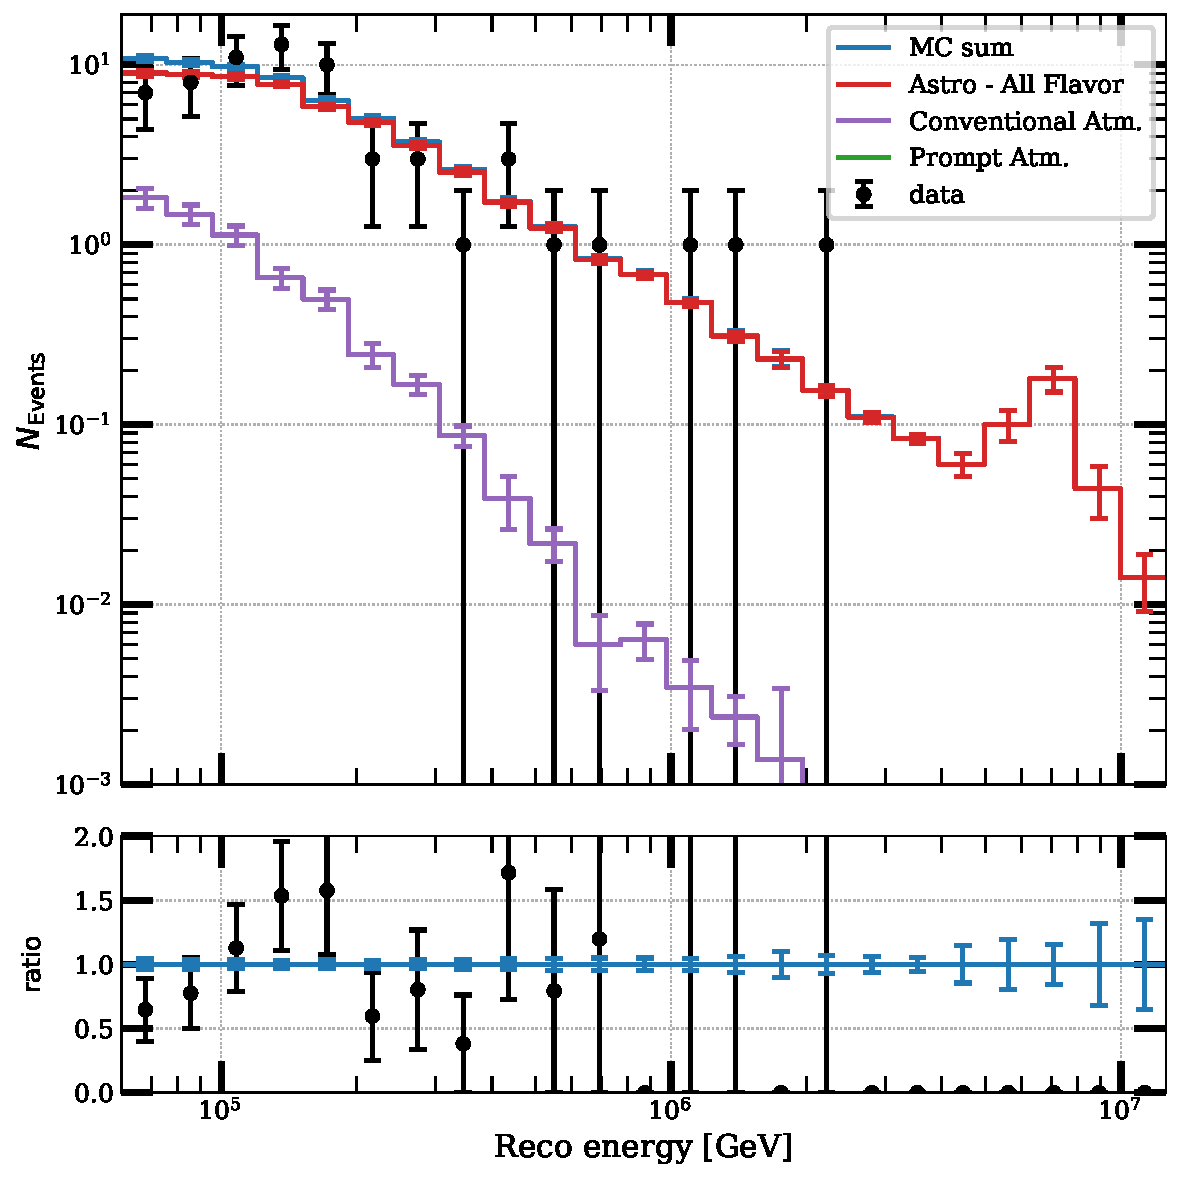
\includegraphics{./figures/results/DataMC_IC86_pass2_SnowStorm_v2_Bfr_Cascades_energy.pdf}
    \end{subfigure}
    \hfill
    \begin{subfigure}[h]{0.7\textwidth}
        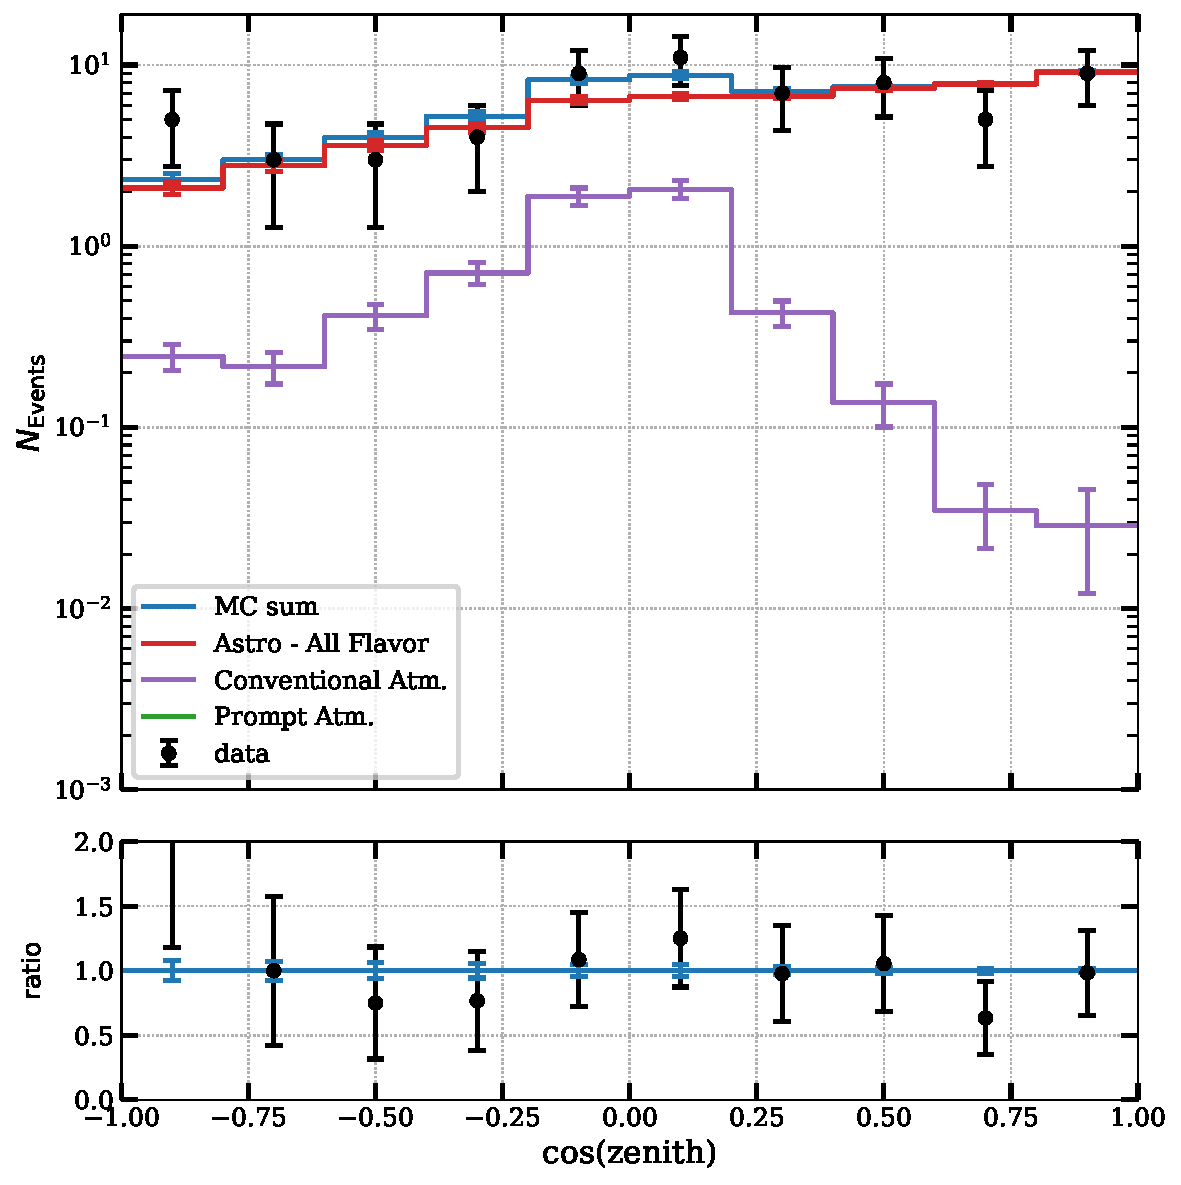
\includegraphics{./figures/results/DataMC_IC86_pass2_SnowStorm_v2_Bfr_Cascades_zenith.pdf}
       
    \end{subfigure}%
    \caption{Observable distributions of the total deposited energy (left) and the zenith angle (right) for events classified as \textbf{single cascades} along with data point positions. Individual components of the fits are produced using bestfit values given in \reftab{bf_signal} and \reftab{bf_nuisance} and MC sum is sum of all of these components. Prompt component is missing on account of bestfit value of 0 for the $\Phi_{\mathrm{prompt}}$.}
    \labfig{Cascades_datamc}
\end{figure*}

\begin{figure*}[h!]
    \begin{subfigure}[h]{0.7\textwidth}
        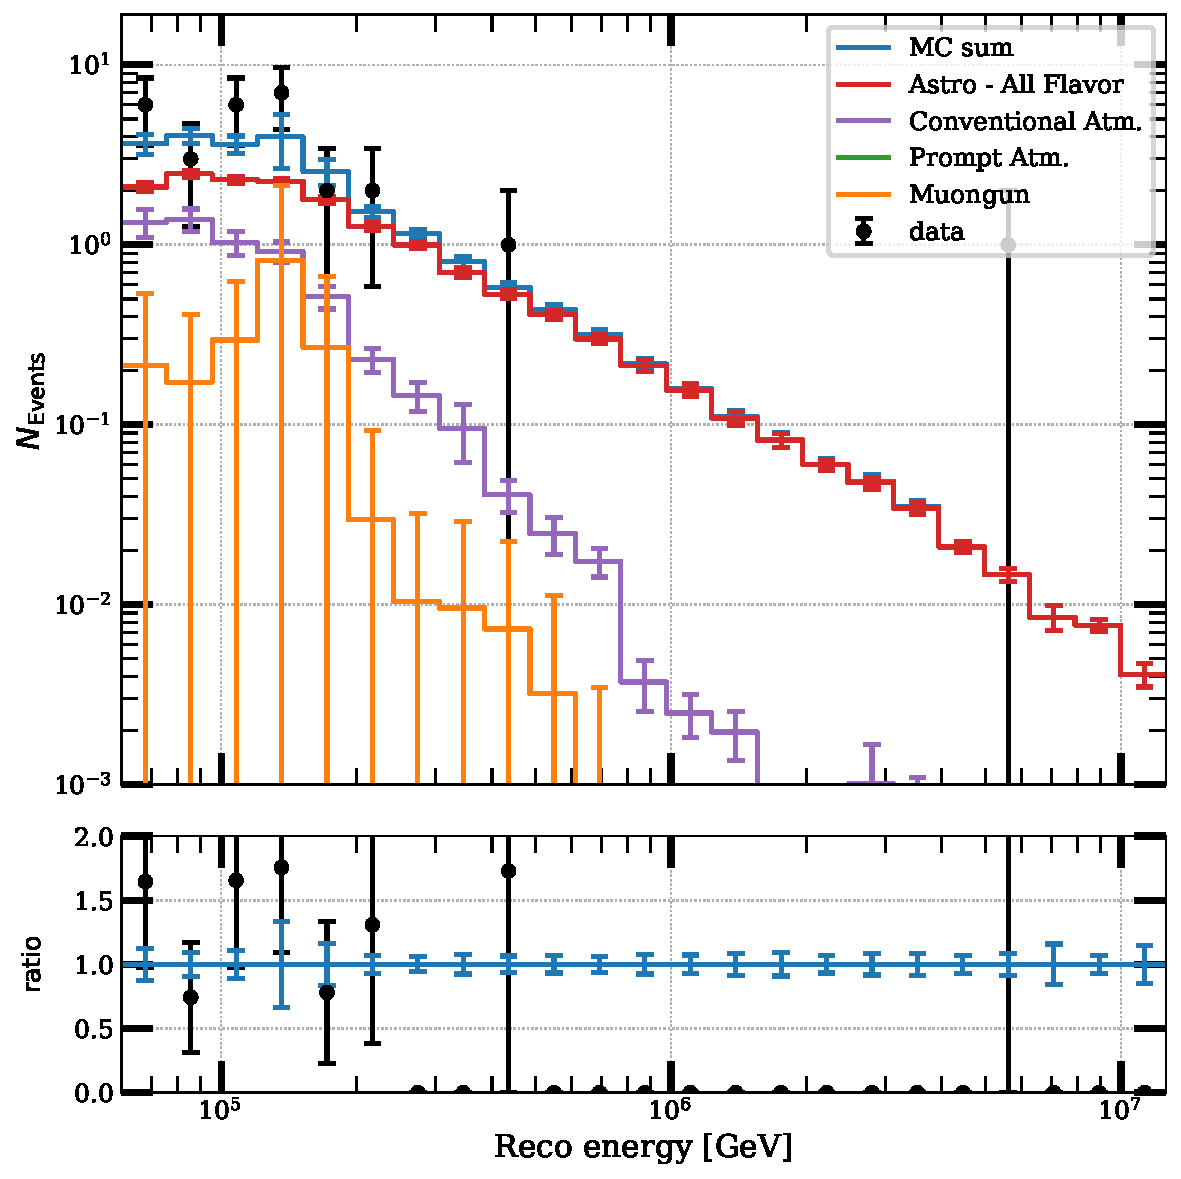
\includegraphics{./figures/results/DataMC_IC86_pass2_SnowStorm_v2_Bfr_Tracks_energy.pdf}
    \end{subfigure}
    \hfill
    \begin{subfigure}[h]{0.7\textwidth}
        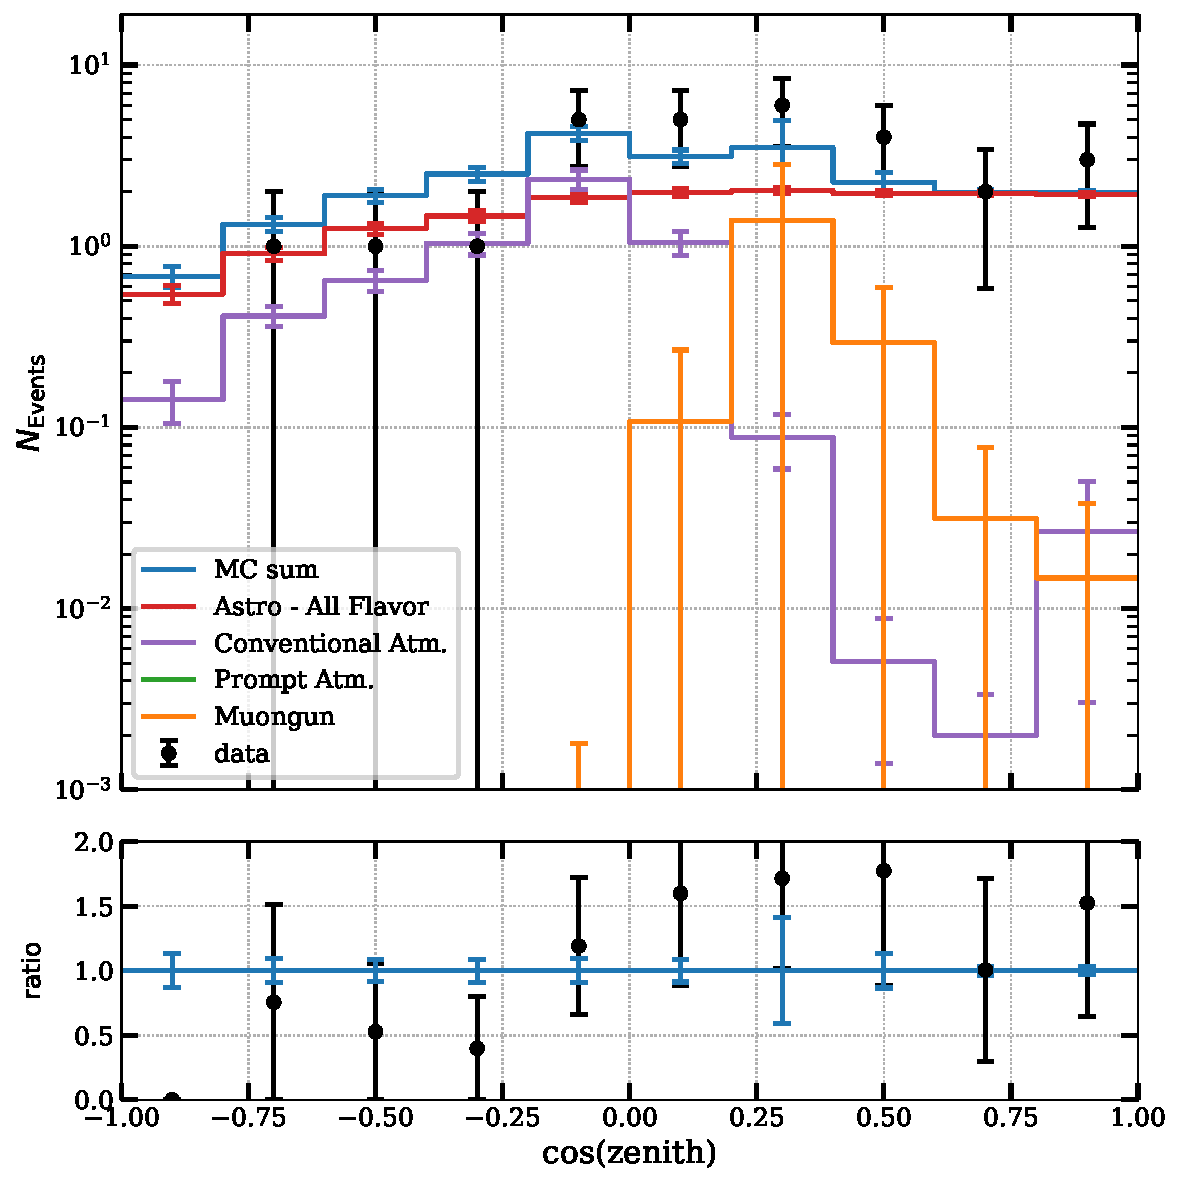
\includegraphics{./figures/results/DataMC_IC86_pass2_SnowStorm_v2_Bfr_Tracks_zenith.pdf}
       
    \end{subfigure}%
    \caption{Observable distributions of the total deposited energy (left) and the zenith angle (right) for events classified as \textbf{tracks} along with data point positions. Individual components of the fits are produced using bestfit values given in \reftab{bf_signal} and \reftab{bf_nuisance} and MC sum is sum of all of these components. Prompt component is missing on account of bestfit value of 0 for the $\Phi_{\mathrm{prompt}}$.}
    \labfig{Tracks_datamc}
\end{figure*}
\newpage
\reffig{double_datamc} illustrates the distribution of reconstructed energy (left) and reconstructed length (right) for events classified as double cascades in the 12 years of HESE data. In the second energy bin, there is an overfluctuation, but it's challenging to incorporate this as a feature due to the large uncertainties in both the monte carlo and data. An interesting feature of the fit can be seen in the conventional component distribution. The application of gradient correction as an additive factor per component indicates that systematics are trying to adjust this component to account for the excess of double cascades at low energy and high length. This suggests that due to fewer statistics compared to tracks, there is more variability in this parameter across the double cascade bins.  Another noteworthy observation is that one event, although close to 100 TeV, has a large length, suggesting that it is a misclassified track. This particular event demonstrates Energy Confinement near the edge (0.97), a cut that is supposed to differentiate between a double cascade and a track, but not quite above the threshold to be a track (0.99). And hence, the event passed all the cuts and ended up being classified as a double cascade. This becomes more evident in 2D distribution of energy and length in \reffig{LvsE_datamc}, where this event clearly ends up in a  background dominated region of the PDF (see \ref{sec:PID} for signal and background pdfs of double cascades). 


\begin{figure*}[h]
    \begin{subfigure}[h]{0.7\textwidth}
        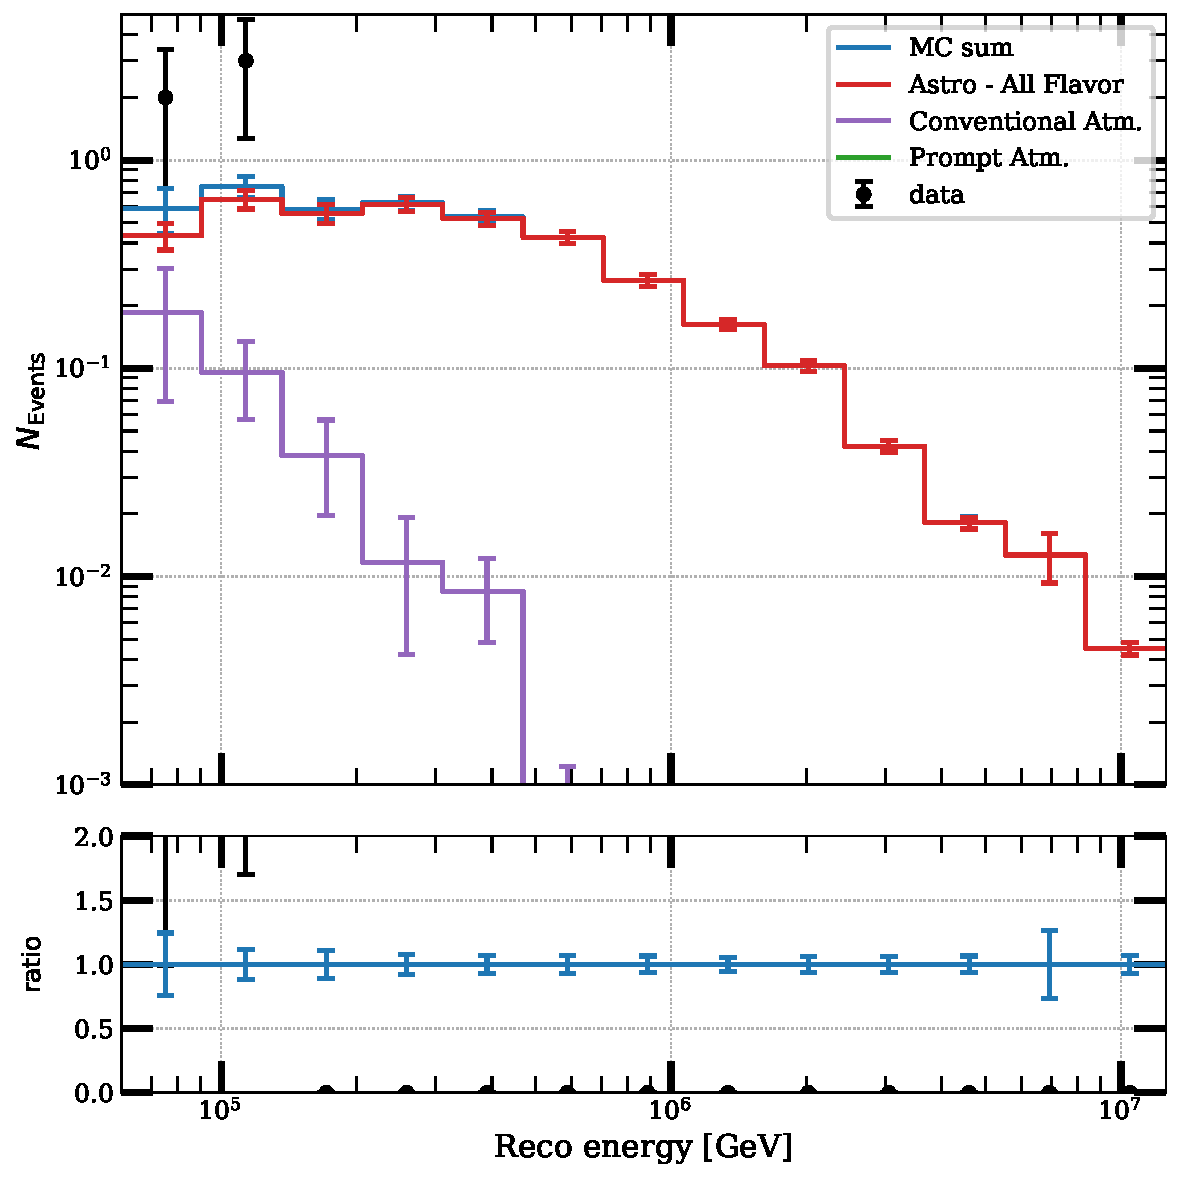
\includegraphics{./figures/results/DataMC_IC86_pass2_SnowStorm_v2_Bfr_DoubleCascades_energy.pdf}
    \end{subfigure}
    \hfill
    \begin{subfigure}[h]{0.7\textwidth}
        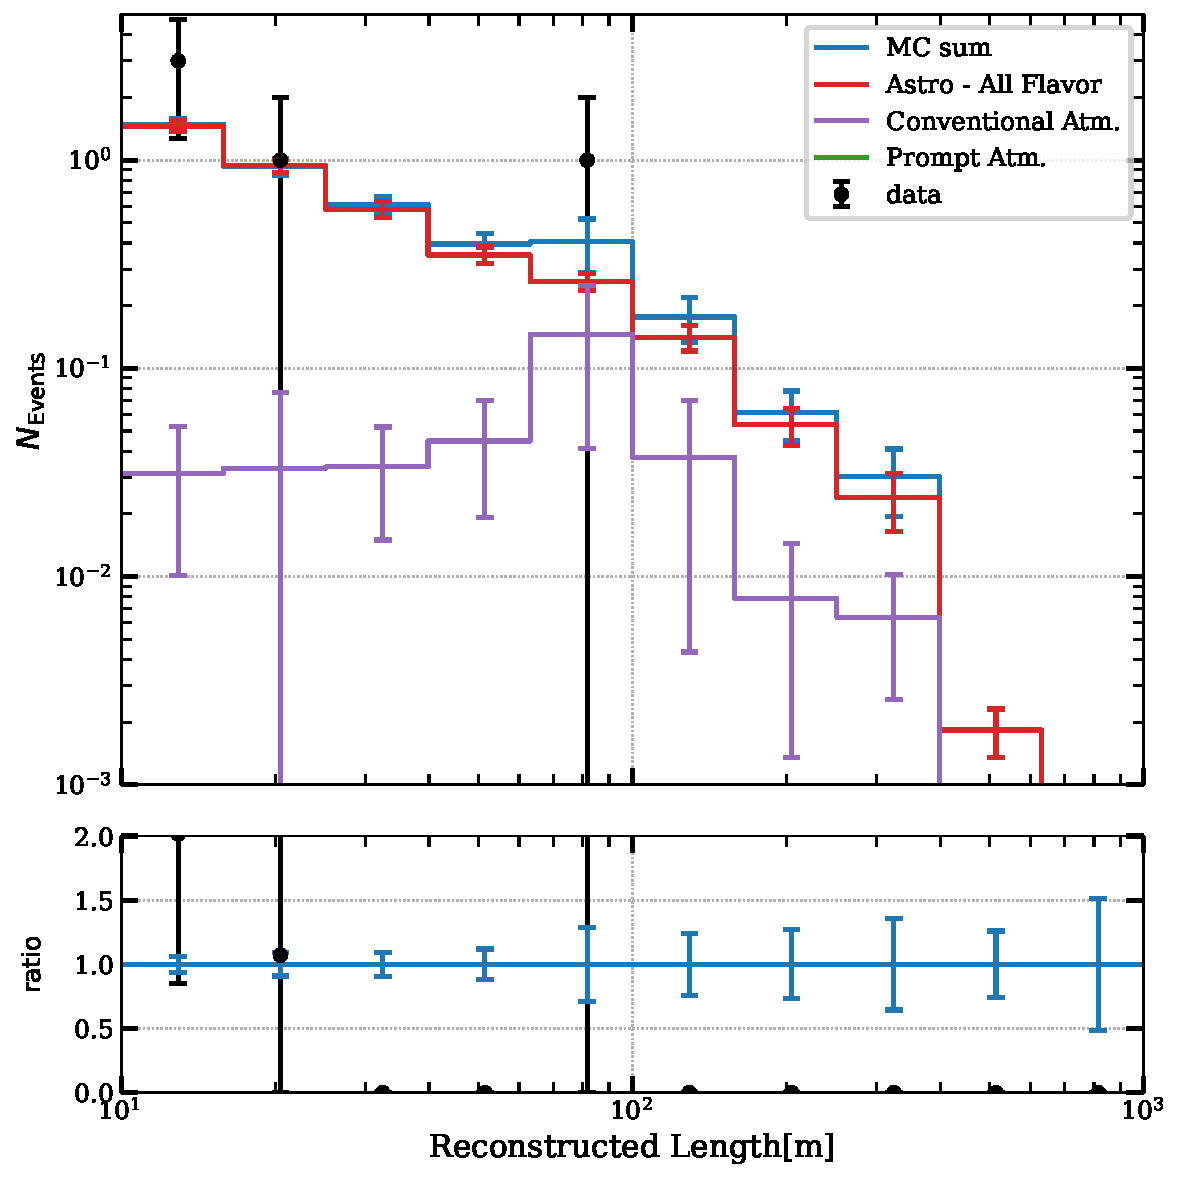
\includegraphics{./figures/results/DataMC_IC86_pass2_SnowStorm_v2_Bfr_DoubleCascades_zenith.pdf}
       
    \end{subfigure}%
    \caption{Observable distributions of the total deposited energy (left) and the reconstructed length (right) for events classified as \textbf{double cascades} along with data point positions. Individual components of the fits are produced using bestfit values given in \reftab{bf_signal} and \reftab{bf_nuisance} and MC sum is sum of all of these components. Prompt component is missing on account of bestfit value of 0 for the $\Phi_{\mathrm{prompt}}$.}
    \labfig{double_datamc}
\end{figure*}
The figure \reffig{LvsE_datamc} illustrates a two-dimensional PID pdf of reconstructed double cascade events, based on the best-fit values described in the tables. The vertical lines demonstrate how quickly the single-cascade background decreases with length. For instance, 68\% of misclassified single cascades have reconstructed double-cascade lengths of less than $\sim 14$ m, 90\% have lengths below $\sim  20$ m, and only 1\% have lengths exceeding $\sim 25$ m. Two of the data events are outside the 68\% region, but one of these events is still within the signal region indicated by white lines. The event with a reconstructed length of approximately 95 m but less than 80 TeV energy is clearly in the background region. Another important observation from this figure is the lack of smoothness expected from PDFs when performing forward folding fits. The gradients are applied as an additive correction per bin, to allow detector systematic variations in the fit. This in turn can significantly change the per bin expectations, making the distributions more fluctuating.
\begin{figure*}[h]
    \begin{subfigure}{0.8\textwidth}
        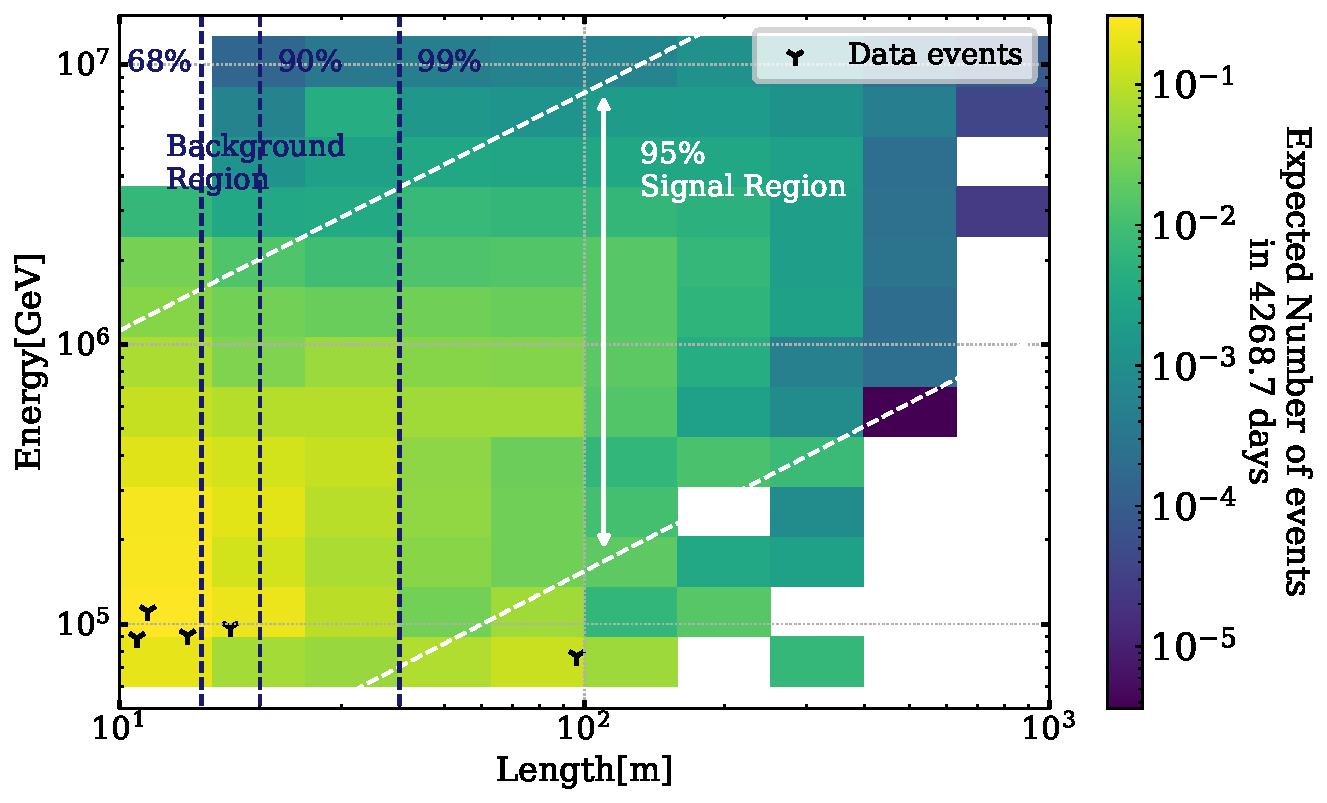
\includegraphics{./figures/results/DataMC_IC86_pass2_SnowStorm_v2_Bfr_DoubleCascadesLvsE_2D_withData.pdf}
    \end{subfigure}
    
    \caption{Two-dimensional distribution of reconstructed energy vs reconstructed double cascade length of the monte carlo events classified as double cascades. Monte carlo sum is produced using all the bestfit parameters from the \reftab{bf_signal} and \reftab{bf_nuisance}. Position of the data events are marked with \wye[rotate=180]. Signal (white) and Background (dark blue) dominated regions are marked with their respective percentiles.}
    \labfig{LvsE_datamc}
\end{figure*}

\begin{marginfigure}
    
    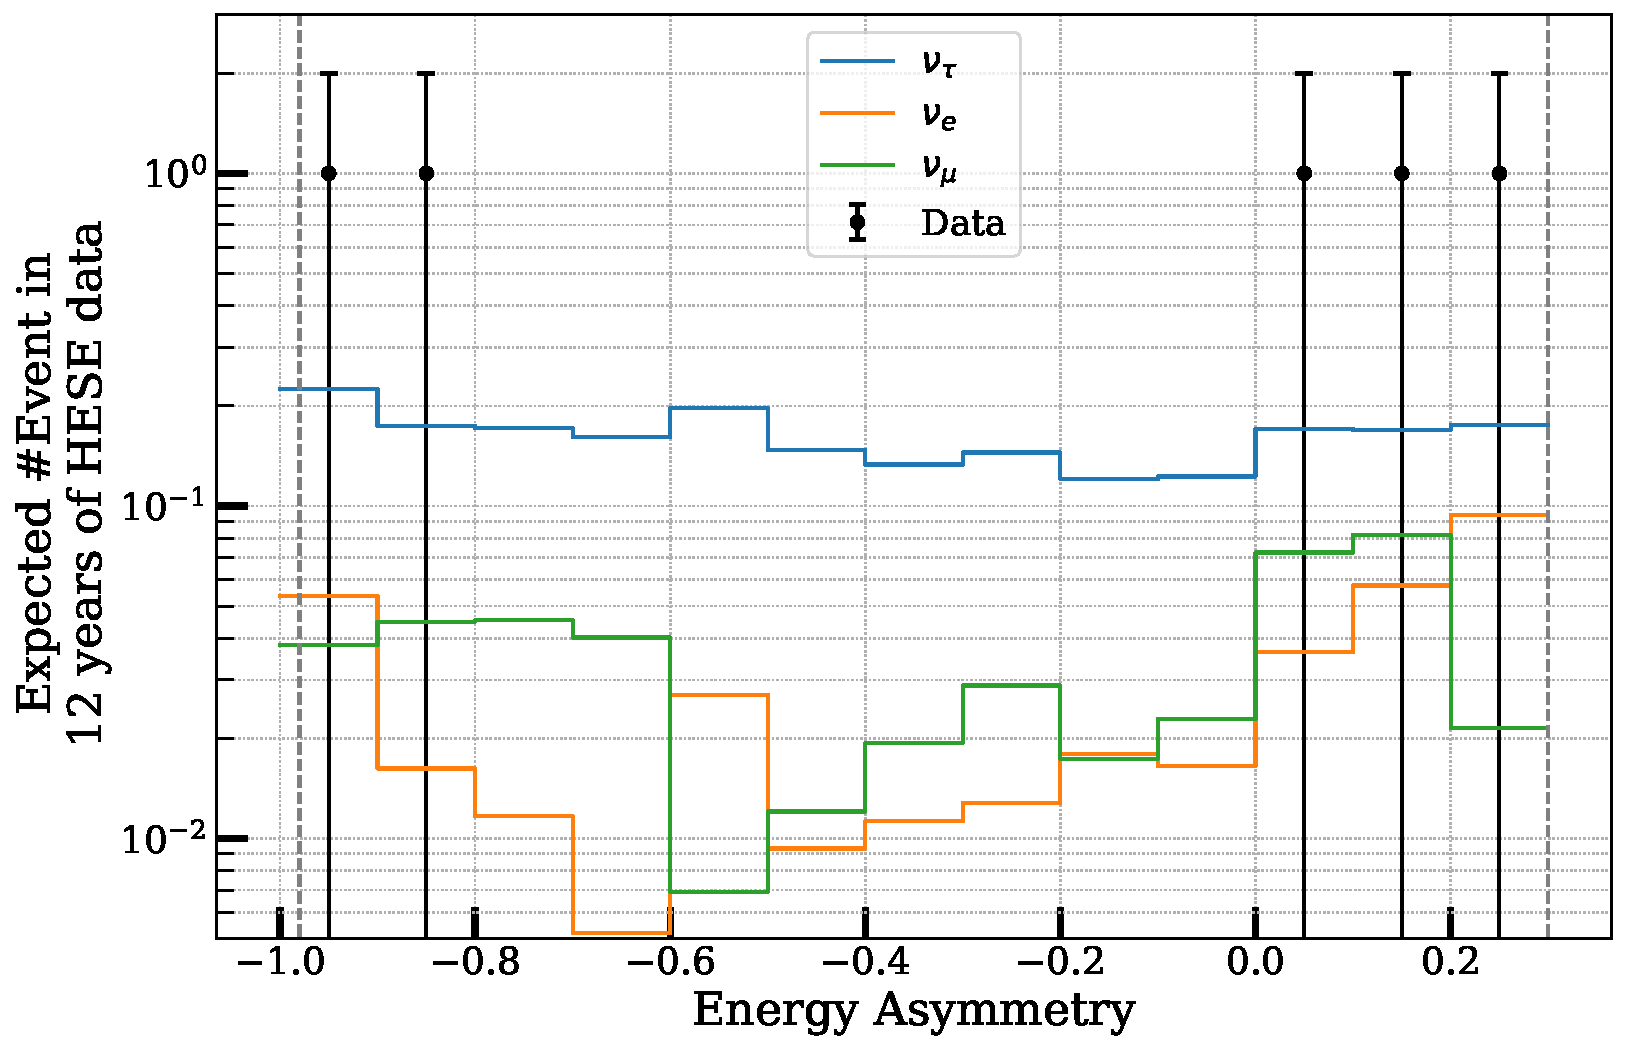
\includegraphics{./figures/results/Energy_ratio.pdf}
    
    \caption{Distribution of reconstructed energy asymmetry, defined as $\mathrm{E}_{\mathrm{A}}=\frac{\mathrm{E}_1-\mathrm{E}_2}{\mathrm{E}_1+\mathrm{E}_2}$, (where $\mathrm{E}_1$ and $\mathrm{E}_2$ are energies of first and second cascades, respectively) at best-fit, along with data events. Distribution is shown for all flavours separately, to emphasis domination of $\nu_{\tau}$ double cascades in the signal region (verticla grey lines).}
    \labfig{Eratio}
\end{marginfigure}

\reffig{Eratio} presents the distribution of the reconstructed energy asymmetry for simulated events in the double-cascade sample, using the best-fit astrophysical and atmospheric spectra. The two vertical lines represent the selection cuts applied to choose the double cascade events, as described in section 4.3. Although two of the 5 events are near the cut edge, they all still fall comfortably within the signal-dominated region of the sample.

\section{Flavour Composition of Diffuse Astrophysical Neutrinos}
\label{sec:flavour_results}
The flavor composition of astrophysical neutrinos is measured using 97 high-energy starting event (HESE) events, which are divided among three morphologies. The profile likelihood scans for the flavor scale factors, specifically $s_{\nu_{e}}$ and $s_{\nu_{\tau}}$, are shown in \reffig{1d_llh}. The results indicate that the tau scale factor ($s_{\nu_{\tau}}$) is only able to reject the possibility of no $\nu_{\tau}$ flux by $1\sigma$ ($-2\Delta \log L=1$), as reflected in the wide contours in the 2D scan shown in \reffig{flavour_comp}. The 1D scans are used to derive $1\sigma$ (68\%) confidence regions, shown in \reftab{bf_signal}. The test statistic $-2\Delta \log L$ compares the global best-fit values of the unconstrained fit to the conditional best-fit values of all remaining model parameters at a fixed scan point. The confidence regions depicted in \reffig{flavour_comp} are calculated using Wilk's theorem \sidecite{Wilks_thm} , as a full Feldman-Cousins construction of the entire flavor composition phase space is computationally demanding (see section \ref{sec:analysis} for details). The agreement of Wilk's theorem is verified by comparing the coverage of the test statistic distribution from Monte Carlo pseudo-experiments to the coverage of a $\chi^2$-distribution. A large fraction of the flavor composition phase space is found to be slightly over-covered, indicating that Wilk's theorem yields a conservative confidence region. Although a part of the 90\% confidence region seems to suffer from slight under-coverage, the $\chi^2$-approximation is deemed sufficient for presenting the measurement result in \reffig{flavour_comp}. 
\begin{figure}
    
    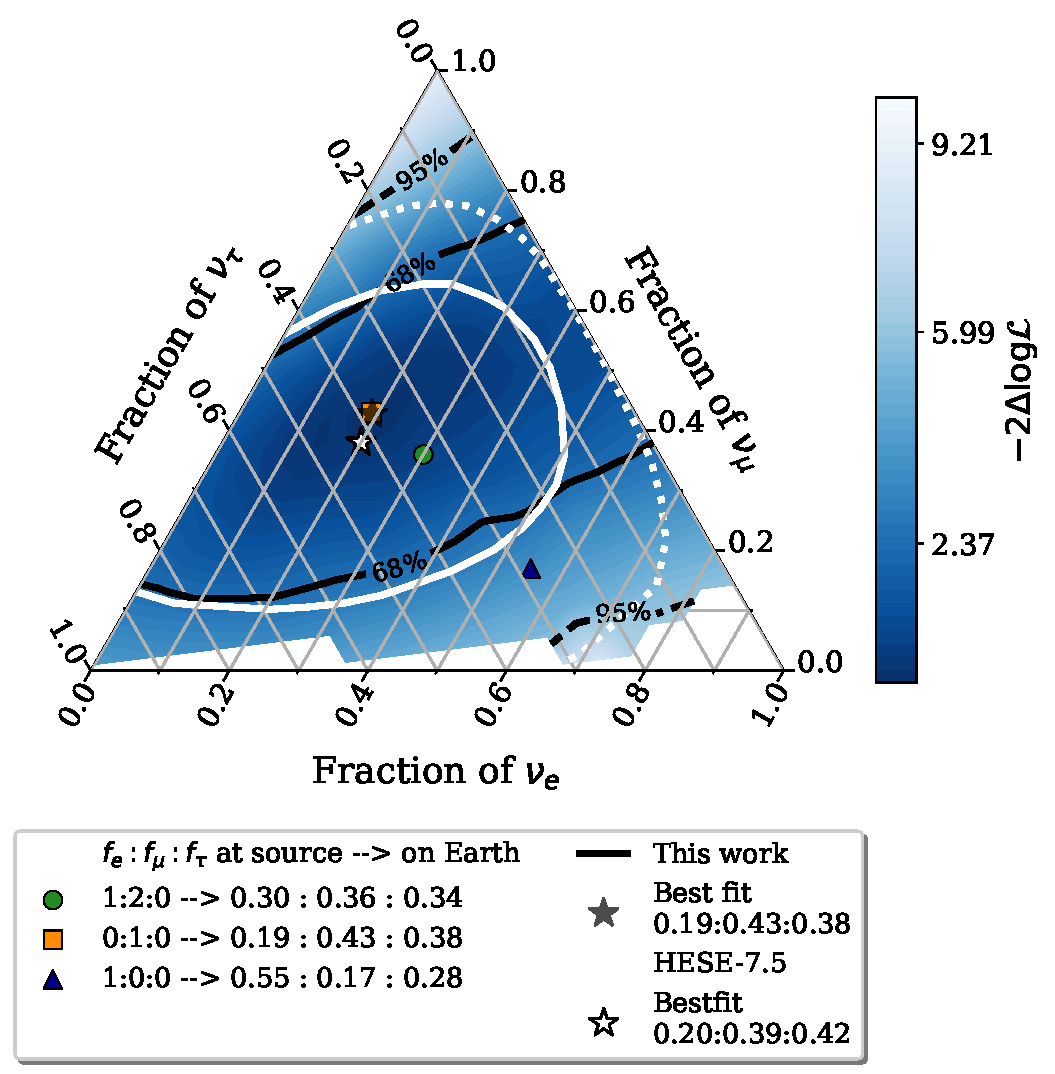
\includegraphics{./figures/results/HESE12_fancy_coverage_say_withhese7.pdf}
    \caption{A 2 dimensional profile likelihood scan of the astrophysical neutrino flavor composition at Earth using 12 years of HESE data, classified in three event morphologies (see text for details). Each point on the triangle corresponds to a flavor composition of $\nu_e : \nu_{\mu} : \nu_{\tau}$ which can be read off the axes along the tick directions specified. The best-fit flavor composition of 0.19 : 0.43 : 0.38 is indicated with a white star. The white solid and dashed lines represent the 68\% and 95\% confidence regions, respectively, obtained from the $\chi^2$-approximation using Wilk's theorem. Three flavor compositions expected at Earth from different source scenarios are also marked (\ref{sec:cosmic_nu}). The best-fit flavor composition of a previous measurement that used 7.5 years of HESE data is indicated in grey star, with the 68\% and 95\% confidence regions represented by the grey solid and dotted lines, respectively \cite{Juliana_paper}.}

    \labfig{flavour_comp}
\end{figure}

\begin{figure*}[h!]
    \begin{subfigure}[h]{0.7\textwidth}
        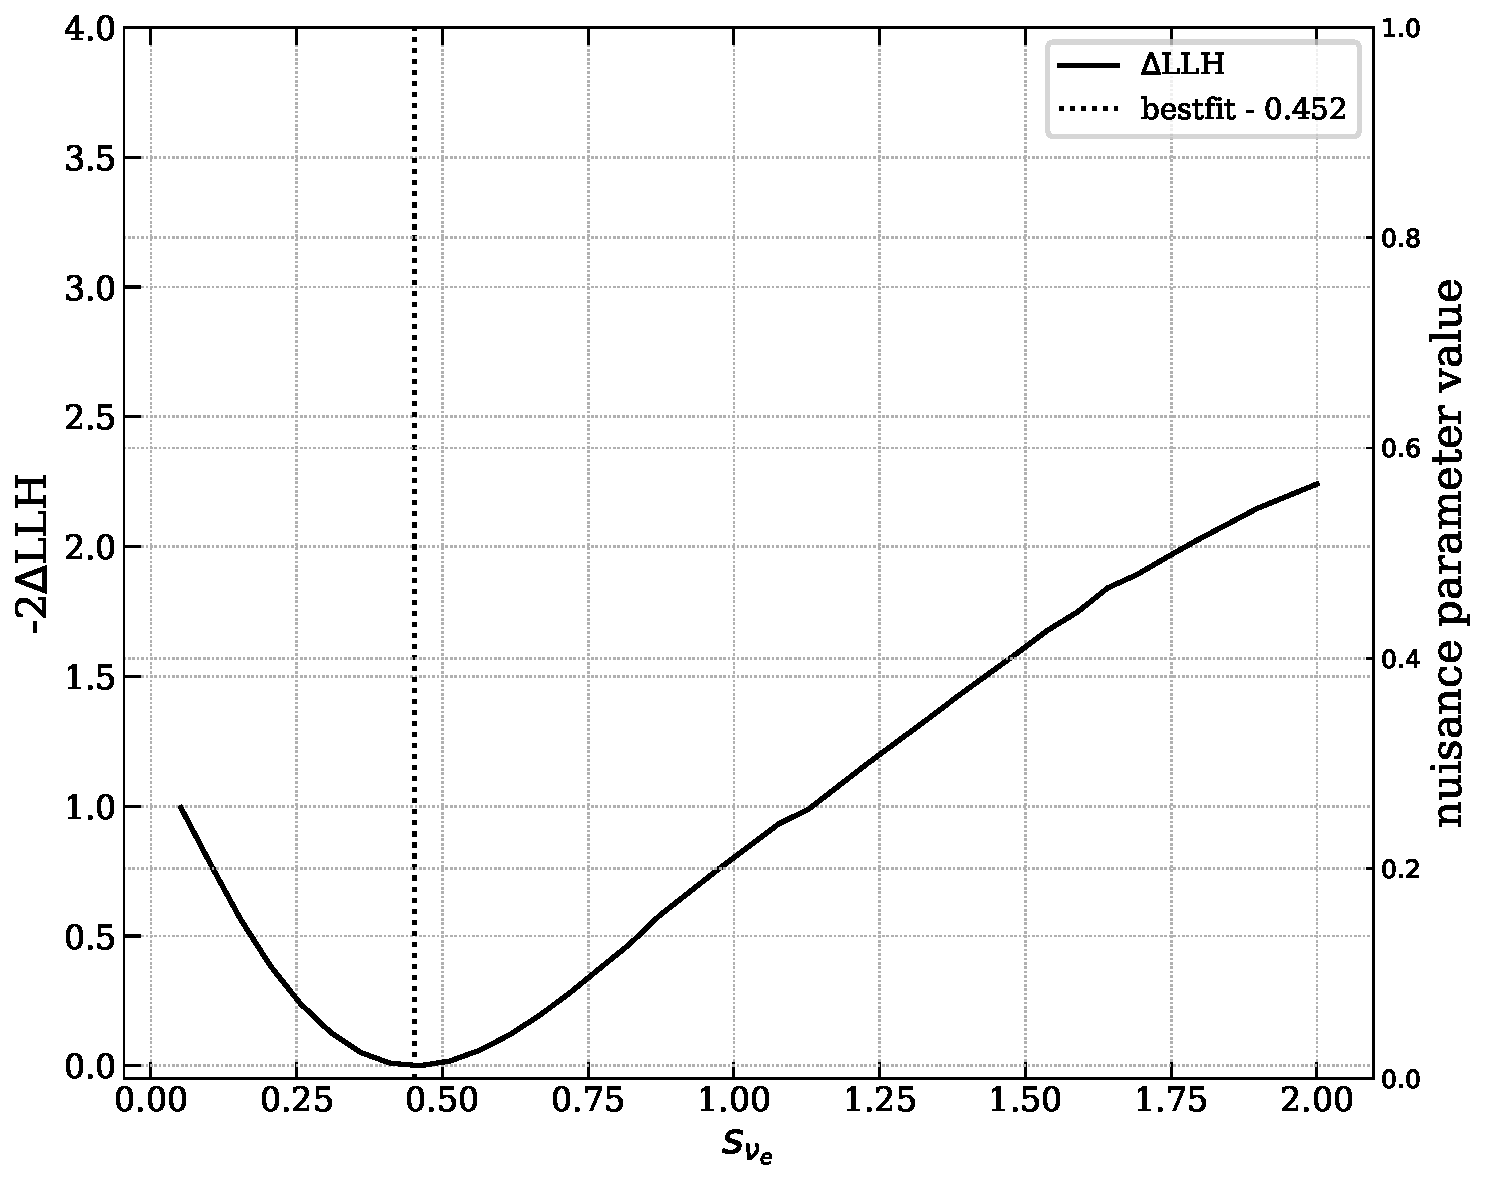
\includegraphics{./figures/results/profile_scan_astro_nue_ratio.pdf}
    \end{subfigure}
    \hfill
    \begin{subfigure}[h]{0.7\textwidth}
        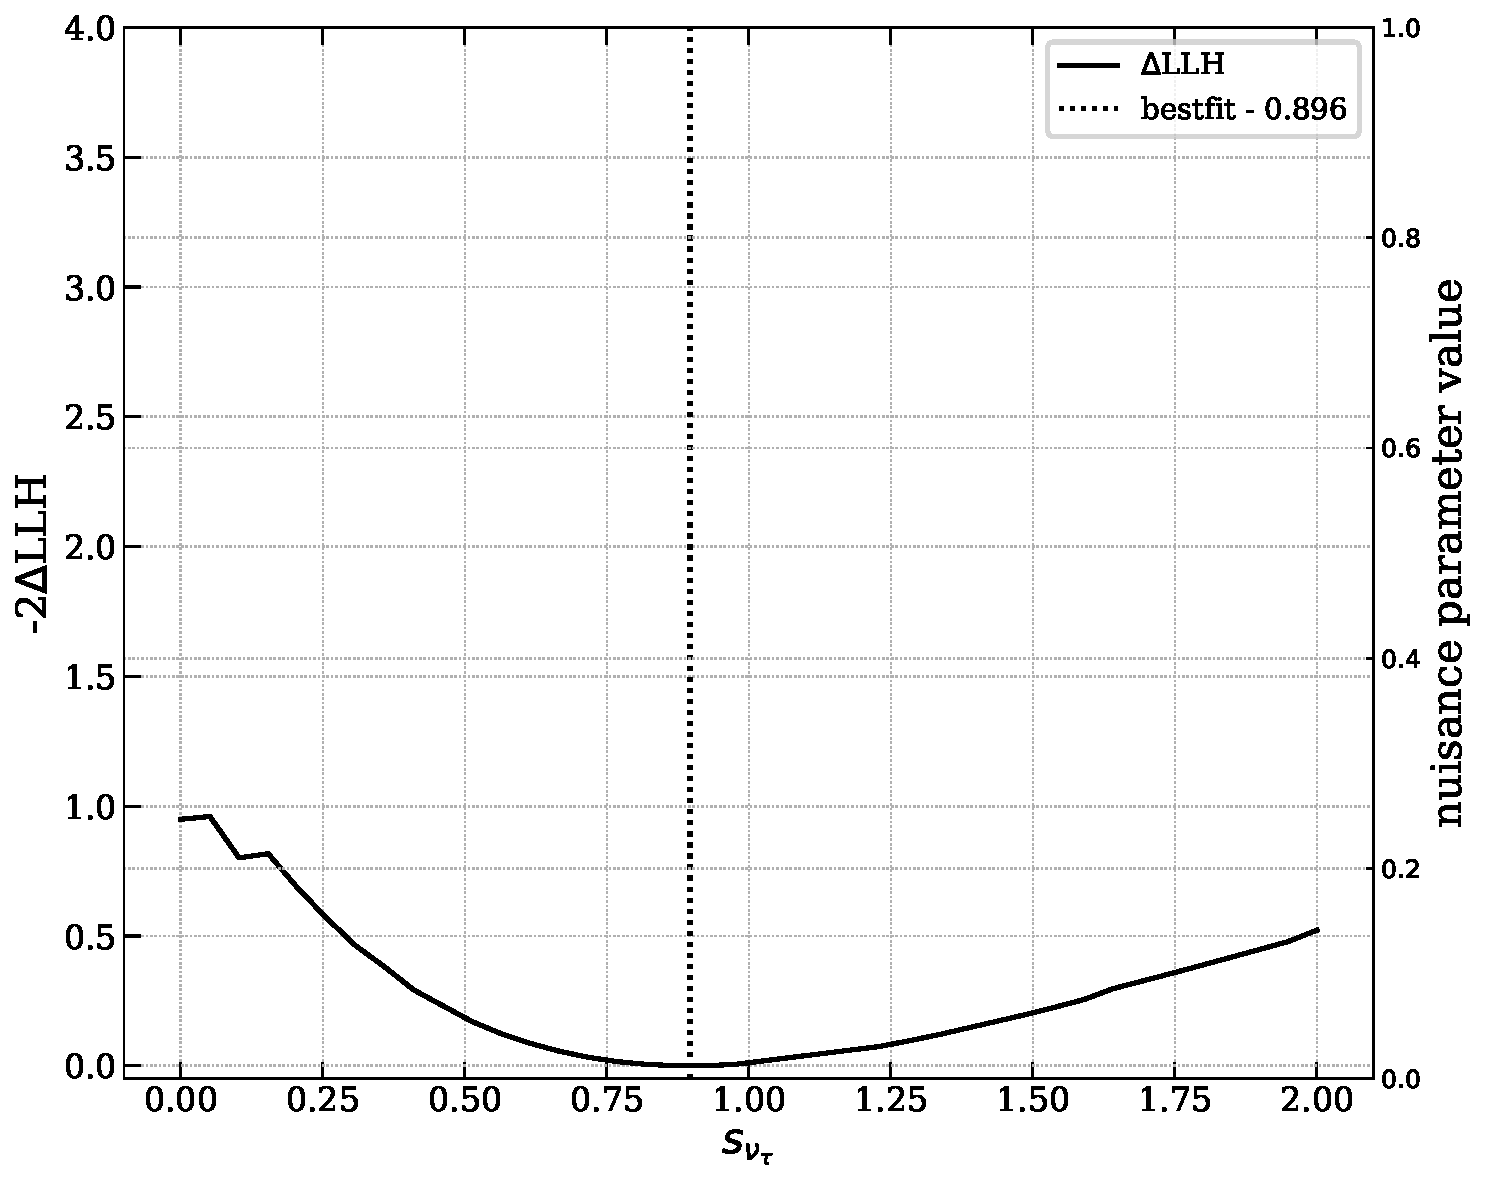
\includegraphics{./figures/results/profile_scan_astro_nutau_ratio.pdf}
    \end{subfigure}
    
    \caption{1 dimensional profile likelihood scan of flavour scale factors $s_{\nu_{e}}$ (left) and $s_{\nu_{\tau}}$ (right). Solid black line corresponds to the profile likelihood, defined by the likelihood ratio $-2\Delta\mathrm{log}\mathcal{L}$ comparing a fixed value to the best-fit value (denoted by dotted line).}
    \labfig{1d_llh}
\end{figure*}

\subsubsection{Why are the limits worse than the previous measurements?}

The best-fit flavor composition $\nu_e:\nu_{\mu}:\nu_{\tau} = 0.19:0.43:0.38$ aligns well with the previous measurement \sidecite{Juliana_paper} of $\nu_e:\nu_{\mu}:\nu_{\tau} = 0.20:0.39:0.42$ (grey lines in \reffig{flavour_comp}). However, with 4 more years of data, which includes more double cascade events, it raises the question of why the limits are not as good. The reason is quite simple, the grey contours are derived using an extended likelihood, based on density estimates by producing a large number ($\sim10^6$ events per particle) of resimulations of 2 classified double cascades to assess the \textbf{tauness} . A dedicated algorithm (\texttt{RODEO}) was developed and used to compute the density estimate for sparse datasets produced from these resimulations in multiple dimensions (see \sidecite{Juliana_thesis} for details). This updated likelihood can be seen as the unbinned, higher-dimensional version of evaluating the contributions of signal-like and background-like events, which was carried out in a two-dimensional binned way (just as done for the analysis presented in this thesis).\marginnote{\begin{kaobox}[title=\textbf{\emph{tauness}}]
    "Tauness" refers to the Bayesian posterior probability that an event is derived from a $\nu_{\tau}$ interaction. This can be approximated by analyzing the fraction of events in close proximity to the reconstructed properties of the data events, which are anticipated to result from $\nu_{\tau}$ interactions. In essence, tauness provides insight into the probability of each double cascade originating from a $\nu_{\tau}$ interaction compared to any other type of interaction.
\end{kaobox}}  Because of this, the limits one should actually compare with the previous measurement should be the one derived using \emph{the non-extended likelihood}, which is the same likelihood and PDF setup used for this iteration of the analysis. \reffig{HESEall68} shows such a comparison. The best-fit flavor composition $\nu_e:\nu_{\mu}:\nu_{\tau} = 0.19:0.43:0.38$ measured using this analysis (black lines) aligns well with the previous measurement of $\nu_e:\nu_{\mu}:\nu_{\tau} = 0.29:0.43:0.28$ (blue lines) using the same likelihood. Although not significantly, the limits derived from this iteration do get better along the $\nu_{\mu}$ fraction. Only 68\% limits are shown, without the likelihood space to keep the plot easy to read.

\begin{figure}[h!]
    \caption{The best-fit flavor composition of 0.19 : 0.43 : 0.38 (black), using 12 years of HESE data (this work) compared with the best-fit flavor composition of a previous measurement that used 7.5 years of HESE data \cite{Juliana_paper}. Comparison is shown by usingth esame likelihood formulation (none extended likelihood without resimulations, see text for details). The solid and dashed lines represent the 68\% and 95\% confidence regions, respectively, obtained from the $\chi^2$-approximation using Wilk's theorem. Three flavor compositions expected at Earth from different source scenarios are also marked (\ref{sec:cosmic_nu}).}
    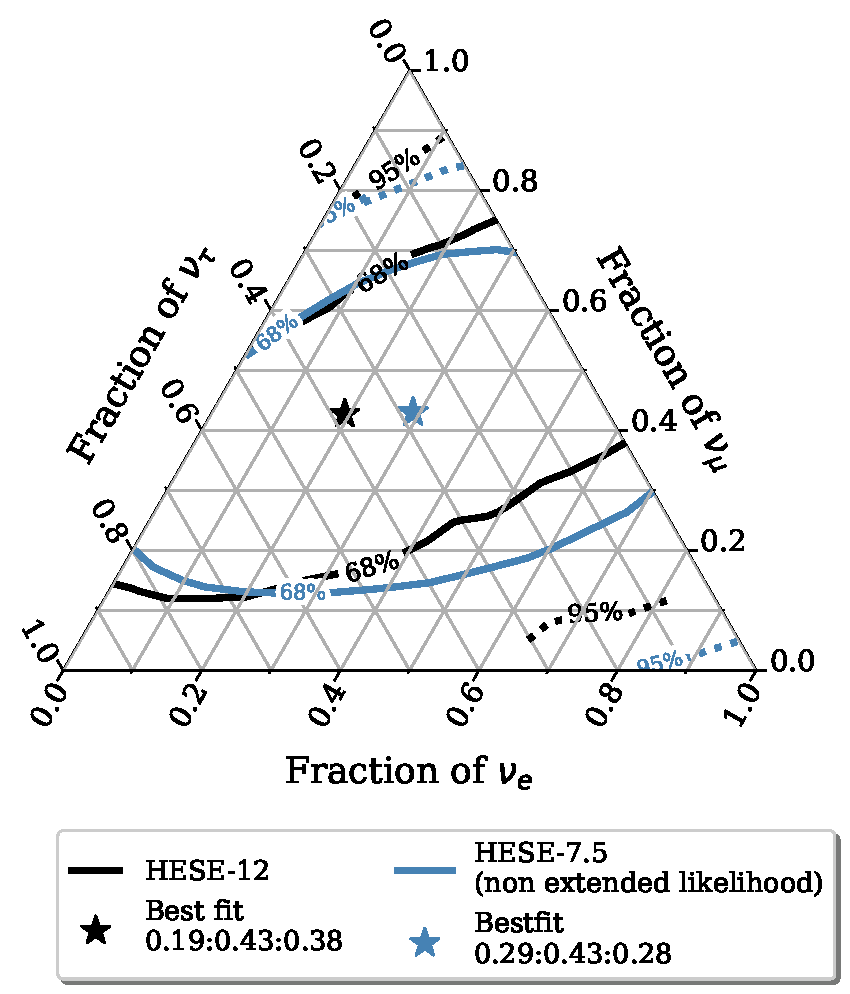
\includegraphics{./figures/results/HESE7and12_nonextendedonly.pdf}


    
    \labfig{HESEall68}
\end{figure}


\subsubsection{Sensitivity at BestFit}
\label{sec:sens_bf}
Please remember the following text:

The setup and all the relevant updates to the sample and selection chain for the analysis presented in this thesis were done using the best-fit values from the previous analysis. The two signal parameters that affect the flavor measurement, especially the $\nu_{\tau}$ fraction and hence the double cascade events, are the index of the primary neutrino energy spectrum $\gamma_{\mathrm{astro}}$ (assuming a single power law) and the normalization. A harder spectrum (low $\gamma_{\mathrm{astro}}$) leads to a higher expected flux, resulting in more expected events, while a softer spectrum (high $\gamma_{\mathrm{astro}}$) leads to a lower flux for samples with a similar effective area. This point was discussed in section \ref{sec:sensitivty} while discussing the sensitivity of the analysis. The analysis setup and sensitivity were shown using a spectrum with an index of 2.87, which is almost identical to the best-fit value for this analysis (2.84) assuming equal partition of the neutrino flavor ($\nu_e : \nu_{\mu} : \nu_{\tau} = 0.33 : 0.33 : 0.33$). Even though the measured flavor ratio is slightly different, the index remains quite close to what the data agrees with, and the estimated sensitivity projected much tighter constraints on 2D flavor measurements, specifically along the $\nu_{\tau}$ axis \todo{cite sensitivity figure here}. To understand the lack of improvement to reduce degeneracy along the $\nu_{e}$/$\nu_{\tau}$ axis, the sensitivity of the flavor measurement was first tested at the best fit.

\begin{marginfigure}
    
    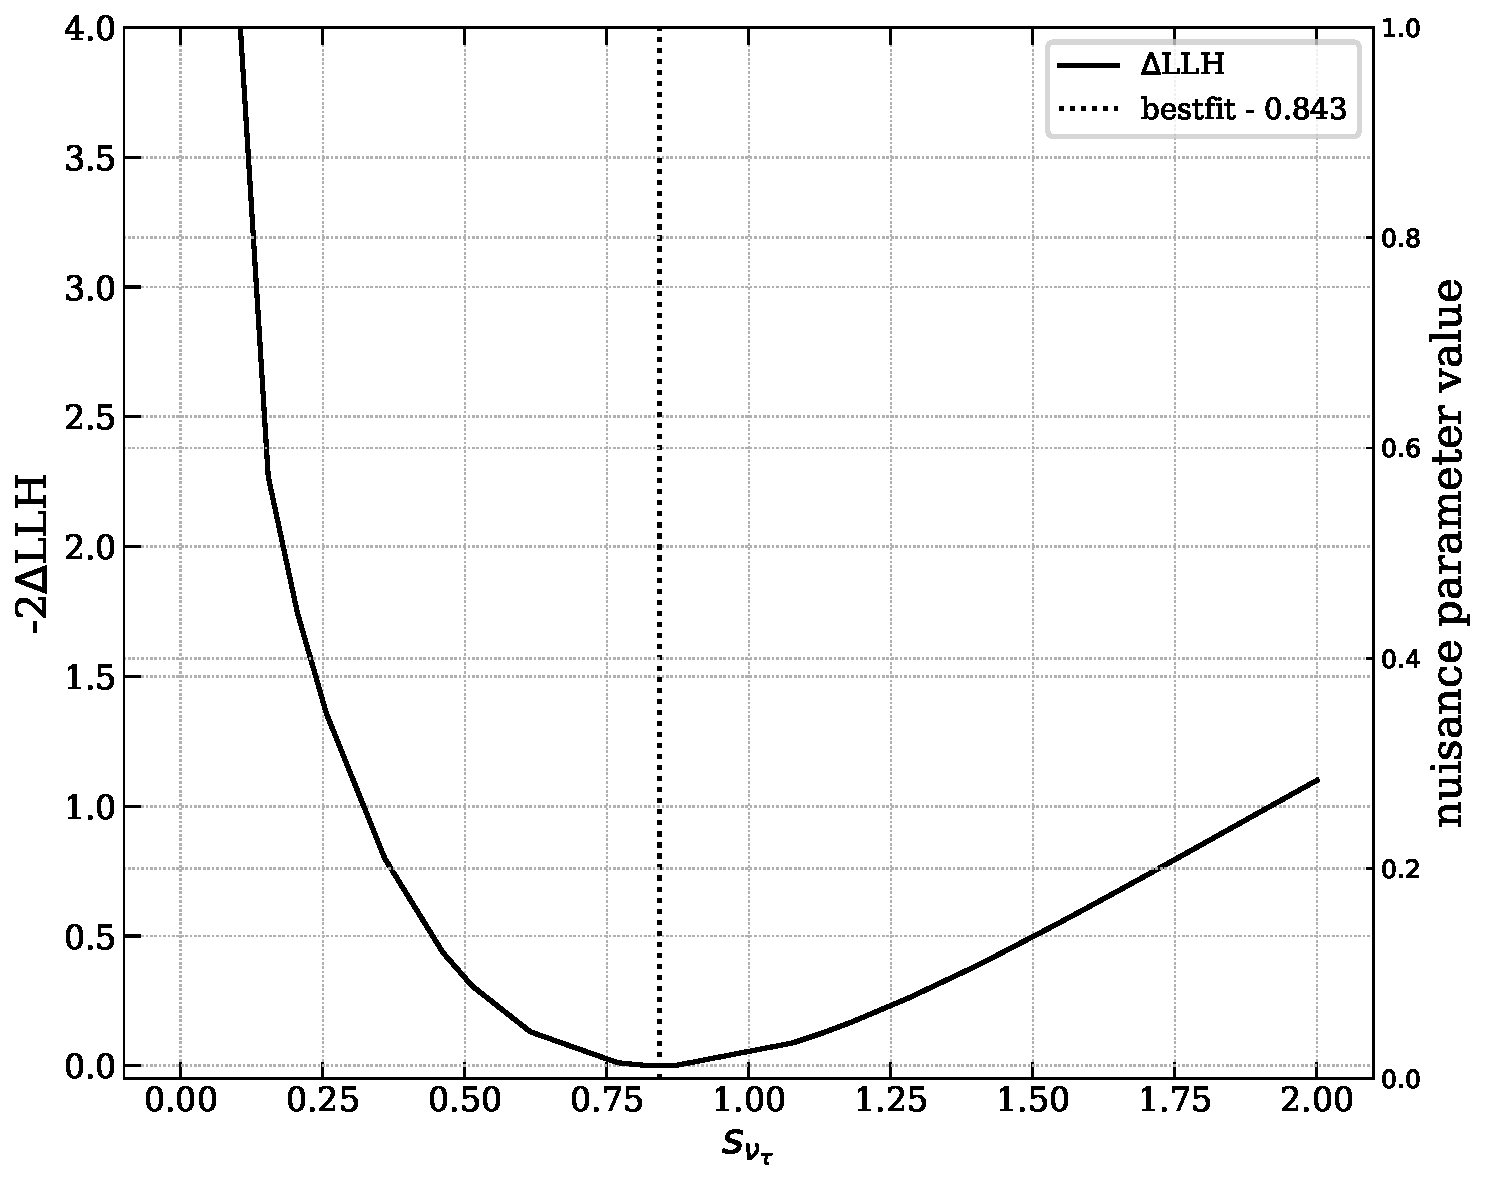
\includegraphics{./figures/results/simulation_profile_scan_astro_nutau_ratio.pdf}
    
    \caption{1 dimensional profile likelihood asimov scan of $\nu_{\tau}$ scale factor, $s_{\nu_{\tau}}$ using \textbf{simulation} injected at bestfit point. Solid black line corresponds to the profile likelihood, defined by the likelihood ratio $-2\Delta\mathrm{log}\mathcal{L}$ comparing a fixed value to the best-fit value (denoted by dotted line).}
    \labfig{profile_llh_nutau_sim}

\end{marginfigure}

The sensitivity of the bestfit analysis is demonstrated in \reffig{PEs}. It is determined by using an asimov dataset \sidecite{asimov} created with the best-fit values of all signal and nuisance parameters from \reftab{bf_signal} and \reftab{bf_nuisance}. For the sake of simplicity in comparison, a Poisson likelihood was utilized, as SAY likelihood tends to yield more conservative limits (refer to the appendix for some comparisons). The objective here is to examine the most ideal scenario. Moreover, constructing pseudotrials where data is drawn from SAY likelihood is not straightforward, therefore, to maintain consistency in comparisons, all fits depicted in \reffig{PEs} are computed using Poisson Likelihood. Consequently, the 68\% data limits displayed on the same plot (black line) are narrower compared to those shown in \reffig{flavour_comp}. Additionally, there is a slight shift in the bestfit point. The key point here is that, given these signal parameters, the analysis is sensitive not only to measure a non-zero $\nu_{\tau}$ fraction, but also to reject it with better significance (approximately $3\sigma$ as shown in \reffig{profile_llh_nutau_sim} - the 1D profile likelihood scan of $s_{\nu_{\tau}}$ for the asimov dataset used to derive the 2D limits shown in \reffig{PEs}). The sensitivity results give rise to three questions:

\textbf{Are data limits reliable?}\\
The contours shown in \reffig{flavour_comp} are based on the assumption that Wilk's theorem holds. This theorem states that the $-2\Delta\mathrm{log}\mathcal{L}$ approximately follows a $\chi^2$-distribution with $k = \text{dof}(\hat{\theta}, \hat{\xi}) - \text{dof}(\theta_t, \xi_t)$, where $\text{dof}(\theta, \xi)$ represents the number of free parameters in the fit. In the case of the flavour fit, there are 2 free parameters - $s_{\nu_{e}}$ and $s_{\nu_{\tau}}$. It is important to note that Wilk's theorem is only valid if the sample size is large and the model parameters are not bounded. However, the HESE sample is relatively small with only a few events passing all selection cuts. Additionally, the available Monte Carlo statistics are not large enough to provide sufficient statistics in every bin of the analysis histograms. Furthermore, the parameters are bounded as the flavour fractions cannot be negative. Therefore, it is essential to verify the validity of Wilk's theorem given these conditions.
     
\textbf{Is deriving sensitivity using an asimov dataset a good choice?}\\
The Asimov dataset is a convenient alternative to generating a large number of pseudo trials for testing a specific realization. Computing the test statistic distribution of both conditional and global best-fit values for each point in the triangle is quite expensive. It should not be assumed that the test statistic value that maximizes the likelihood of the Asimov dataset is always equal to the median of the test statistics derived from the full distribution of various pseudo experiments. Therefore, the next step is to calculate sensitivity using Monte Carlo pseudo experiments.

\textbf{Is the 2 dimesnional monte carlo PDF ideal for the fit to differentiate between signal and background?}\\

Forward-folding fits, as described in section \ref{sec:analysis}, heavily relies on the expected values for each bin of the analysis histograms. It is crucial to choose reliable variables so that the likelihood space looks different for signal and background. For this reason, the analysis variables for double cascade bins are different from those for cascades and tracks. This is because the zenith distribution of astrophysical $\nu_{\tau}$ flux shows no significant variation between signal and background. The PDF used in this case was selected due to the correlation of the Tau decay length ($\mathrm{L}_{\mathrm{dc}}$) with the energy of the second cascade ($\mathrm{E}_{2}$) for double cascades resulting from $\nu_{\tau}$-cc interactions, contributing to the population of signal events along this diagonal \todo{reference PDFs from the analysis chapter}. The 2D Monte Carlo PDF at best fit, shown in \reffig{LvsE_datamc}, contains Monte Carlo events populating the bins along the diagonal. However, the data events are in regions where the background population is expected with nearly equal probability. While drawing data using poisson distribution, fluctuations around the best-fit are considered which in principle should give all possible realisations of the data events ending up in bins with high expectations \sidenote{This was also the motivation beg=hind the resimulations that were performed for the previous iteration of the analysis to measure the flavour composition}. Since data events are observed in bins with not so high expectations as well, it may happen that most pseudo trial histograms would end up not replicating data event distributions. Therefore, in addition to the pseudotrials described earlier, the histograms produced for each trial were checked to see how often the events ended up in a region mostly occupied by background-like events. 

\begin{marginfigure}
    
    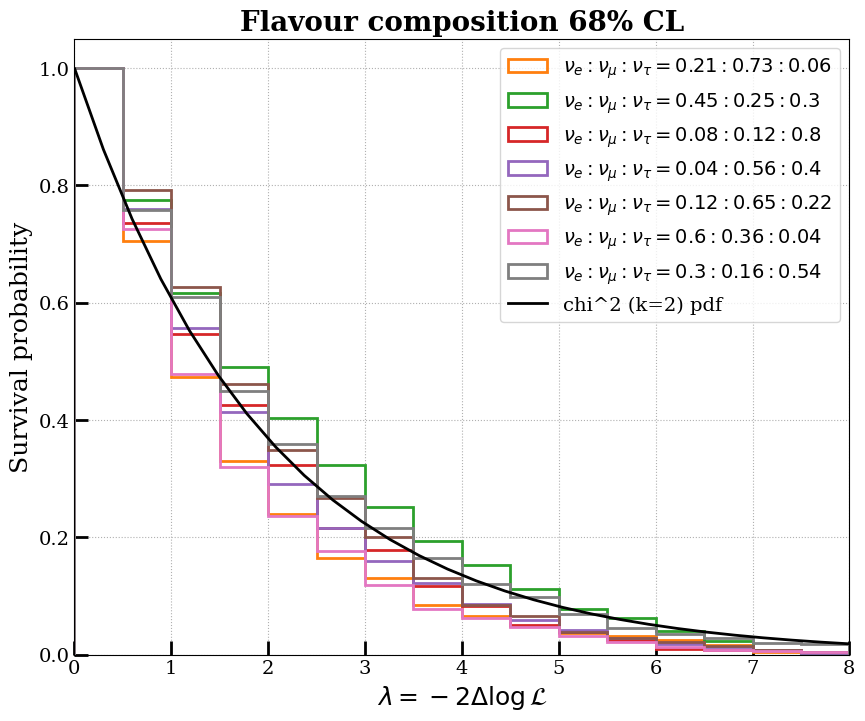
\includegraphics{./figures/results/wilk's test.png}
    
    \caption{Test statistic distribution of the pseudo datasets. All datasets are injected at set of points on 68\% contour (solid white line) of \reffig{flavour_comp} (also shown in legend). a $\chi^2$-distribution with 2 degrees of freedom is also shown (black line) for refernece.}
    \labfig{wilks_68}

\end{marginfigure}

Both of these tests were conducted and their detailed descriptions are provided in Appendix A. The validity of Wilk's theorem was tested for a few points on the 68\% and 95\% contours. This was achieved by generating pseudo datasets (500 trials per dataset), each injected with a specific flavor composition (a point on the contour), while keeping the rest of the fit parameters at their best-fit values. Each trial was fitted twice: once by keeping the parameters fixed at the injection point and once with them free. A likelihood ratio test was performed for each trial by taking the ratio of free to fixed likelihood values. The results are represented in a TS distribution shown in Figure A (for points on the 68\% line). For comparison, a $\chi^2$-distribution with 2 degrees of freedom is also shown (black line). The TS distribution of some points shows a minor shift from the $\chi^2$ (k=2) case, but nevertheless, shows no significant violation of Wilk's theorem.


\begin{figure}[h]
    
    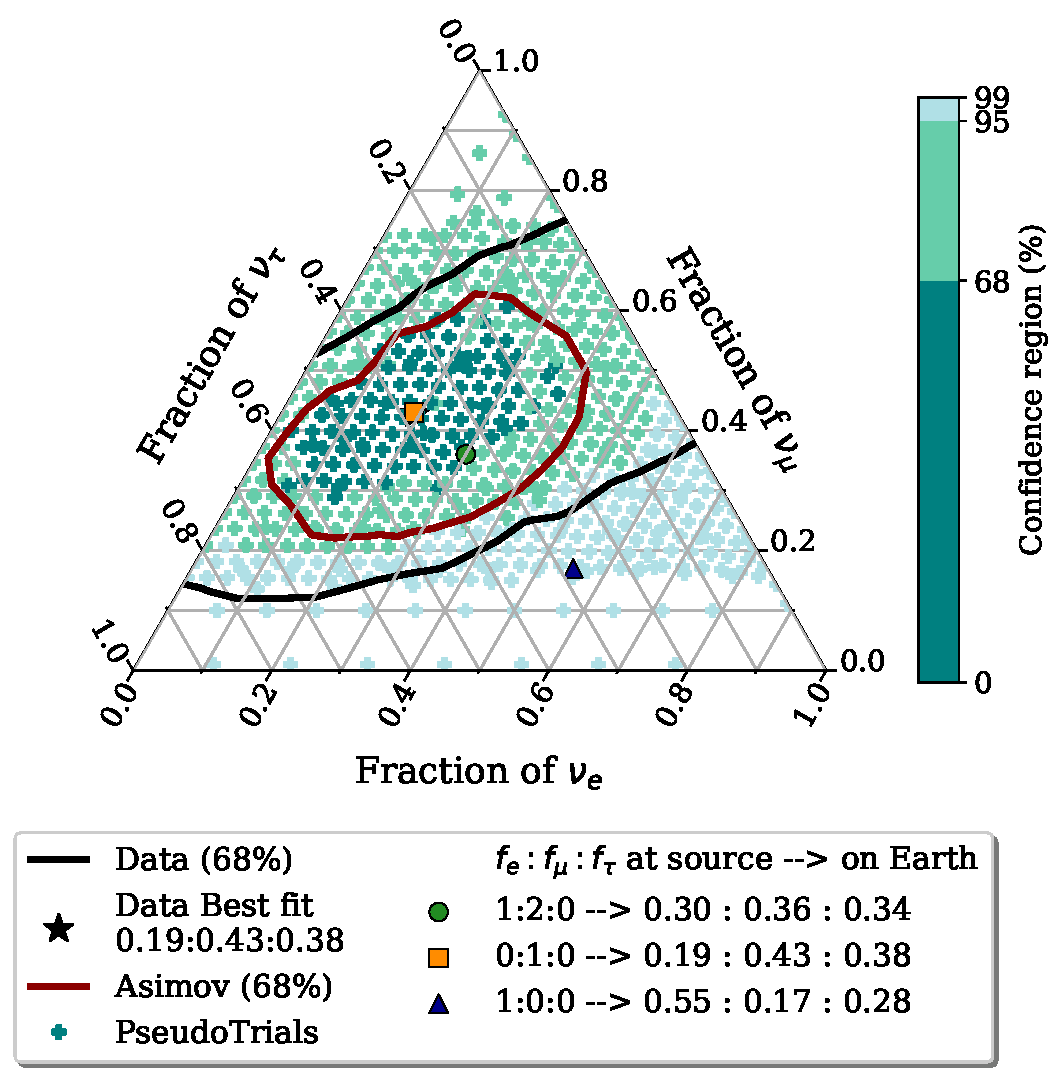
\includegraphics{./figures/results/PE_data_asimov_68.pdf}


    \caption{Comparison of Measured flavoured ratio (black line) with asimov sensitivity(maroon line) and pseudo trials (marked with '+'). Each + represents a pseudo dataset, drawn from flavour composition of that very point. Colorbar shows confidence intervals of each of these points, to reject the bestfit flavour composition of $\nu_e:\nu_{\mu}:\nu_{\tau} = 0.19:0.43:0.38$. All other parameters of the fit are injected at their bestfit values.}
    \labfig{PEs}
\end{figure}

The second test was conducted in a similar way, but this time the fixed point for all trials was kept at the data best-fit point. In Figure B, each point denoted with a marker "+" represents the points for which pseudo datasets were generated. Each dataset was generated by injecting the point denoted with "+" and fitted twice: once by keeping $s_{\nu_{e}}$ and $s_{\nu_{\tau}}$ fixed at the data best-fit values (from \reftab{bf_signal}) and once with them free. This was done to test if the true flavor fraction is what the data fit returns and with what confidence the injected point can be rejected. The result is shown in Figure B. The color scheme shows the confidence level each point has to reject the null hypothesis (data best-fit in this case). As can be seen, the pseudo-trial distribution matches quite well with the Asimov sensitivity. In fact, it predicts even tighter constraints compared to the Asimov case, indicating that neither data limits nor Asimov limits are unreliable.

Lastly, the aforementioned third point was checked. Ideally, one would generate pseudo trials until all the Poisson-distributed events fall within the same region of the PDF as shown in \reffig{LvsE_datamc}. However, this approach was found to be computationally expensive. For instance, each dataset displayed (around 400) in \reffig{PEs} was produced from 500 trials, with each trial fitted twice. On average, each fit took approximately one hour to complete. Therefore, before proceeding, the proportion of PDFs that did not meet the cut criteria was estimated to determine whether using computational resources for further trials was justified. Several tested datasets from different regions of the triangle revealed that, for most datasets, only about 20\% of the 500 trials resulted in final histograms with events concentrated in the lower energy bins. There was no feasible way to generate a sufficient number of trials to reduce statistical errors and set definitive limits. As a workaround, only the small proportion of trials that met the necessary criteria were used to generate the TS distributions, allowing an update of the sensitivity shown in \reffig{PEs}. This updated result is presented in \reffig{PEs_bkg}. As evident from the vanished points, not only were most of the trials excluded, but the confidence intervals also became significantly larger—especially along the $\nu_{\tau}$ axis—aligning more closely with the data limits. This concludes why both asimov sensitivity and pseudo trials in \reffig{PEs} showed such tight constraints. In an ideal case, one can perform resimulations of the 5 double cascade events as it was done for the previous iteration, but this would in turn increase computational resources and was beyond the timeline of work presented in this thesis, hence it was not performed.


\begin{figure}[h]
    
    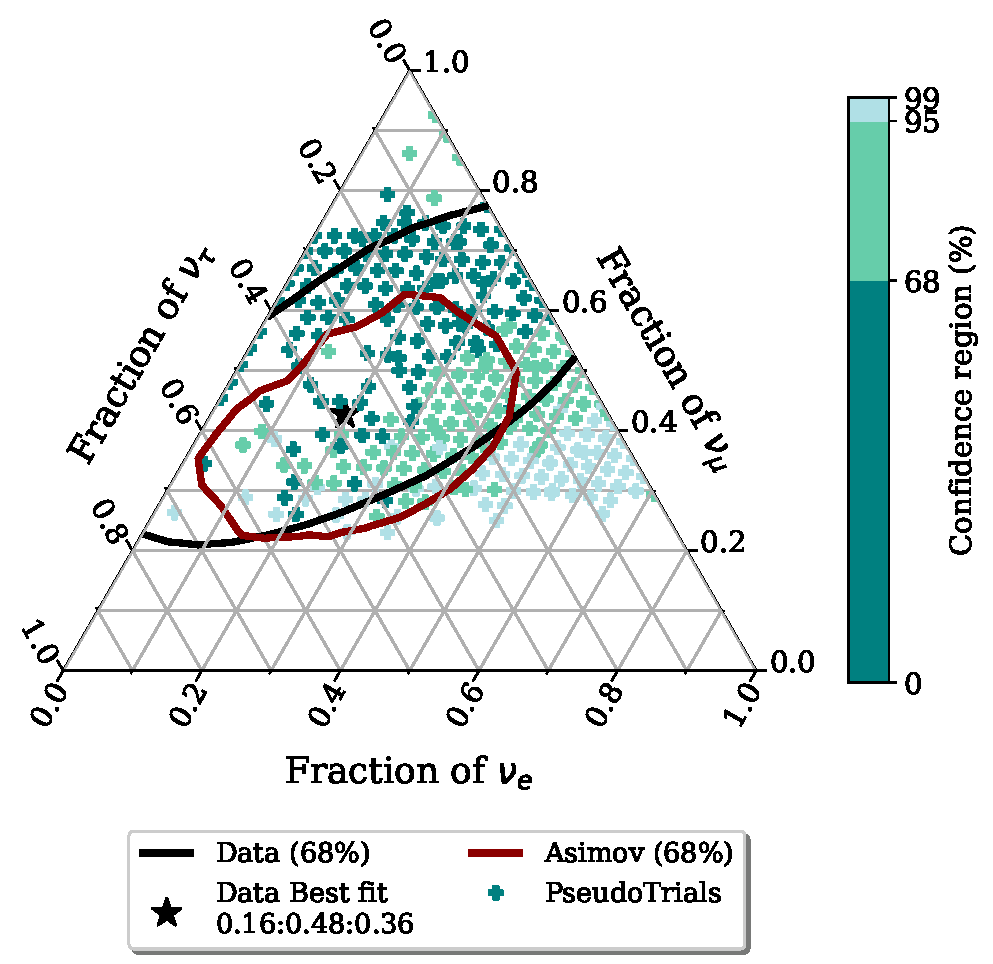
\includegraphics{./figures/results/PE_data_asimov_68_BkgOnly.pdf}


    \caption{Comparison of Measured flavoured ratio (black line) with asimov sensitivity(maroon line) and pseudo trials (marked with '+'). Each + represents a pseudo dataset, drawn from flavour composition of that very point. Colorbar shows confidence intervals of each of these points, to reject the bestfit flavour composition of $\nu_e:\nu_{\mu}:\nu_{\tau} = 0.19:0.43:0.38$. Only trials with final histogram in three lower energy bins are kept in TS distribution. All other parameters of the fit are injected at their bestfit values.}
    \labfig{PEs_bkg}
\end{figure}

\section{Discussion}
\label{sec:results_discussion}

The analysis setup and particle identification methods developed and refined throughout this thesis demonstrate that IceCube is sensitive enough to measure the flavor ratios of the astrophysical neutrino spectrum and set tight constraints. However, more robust techniques, particularly for reconstructing double-cascade events, are needed to produce more reliable Monte Carlo PDFs for these fits. Regarding the measured flavor ratio, as shown in \reffig{Flavour_comp}, although the best fit suggests neutrinos are produced by the muon-damped scenario at high-energy sources, no other source scenarios can be excluded with high significance. The neutron beam scenario ($\nu_e:\nu_{\mu}:\nu_{\tau} = 1:0:0$ at the source, evolving to 0.55:0.17:0.28 on Earth) is disfavored by approximately $1\sigma$ but remains consistent at $2\sigma$.

A specific measurement of the neutrino energy spectrum was not part of the analysis presented here, as the focus was primarily on flavor measurement, with efforts directed toward improving particle identification. Nonetheless, the HESE sample could also be used to measure, and potentially search for, spectral features. Recent independent studies have discovered a spectral break in the neutrino spectrum at around 30 TeV, softening the spectrum at higher energies, which is within the range of this analysis \sidecite{globalfit_icrc,MESE_icrc}. This finding offers insight into why previous measurements targeting different energy ranges produced significantly different spectral indices for a single power-law spectrum \sidecite{HESE7_sample,diffusenumu,cscd_6yr}. Since the HESE sample focuses on high-energy events, where no such spectral features have been observed, and has much lower statistical power than those other samples, no spectral feature searches were attempted during this thesis work.

A less model-dependent approach to describing the astrophysical neutrino flux is the differential unfolding of the energy spectrum. This method divides the flux into energy bins, where each bin is fit independently with a constant $\sim\mathrm{E}^{-2}$ spectrum, rather than assuming a continuous power-law across the entire energy range. Ideally, this unfolding would be performed separately for each neutrino flavor to avoid assuming a uniform spectral shape for all flavors. Measuring the flavor composition as a function of energy would also be valuable, as neutrino production processes are energy-dependent. However, due to the limited statistical power of the current dataset, meaningful results could not yet be obtained.

Finally, improvements in reconstruction methods and more data are necessary for future experiments to shed more light on flavor measurements. Double-cascade reconstruction currently has an upper energy limit, as higher-energy events are only partially contained within the detector due to their geometry. In addition, improved detection hardware could provide better information on photon charge and direction, enhancing the overall reconstruction process. These points, along with the potential for a proposed new generation of neutrino detectors, will be discussed in detail in the next chapter. 


% In particular, various issues encoutered, ice model effects, using high quantum efficiency DOMs, etc need to be studied in more detail. The reconstruction and classification algorithms were desgined and developed while neither detector nor detecting medium was well understood. With more than 10 years of data, the statistical uncertainties are reducing significantly, revealing interesting physics (for both neutrinos and detector). Using all of this new information, the selection can be made more robust against changes like use of DOMs, icemodels etc. 

% \setchapterpreamble[u]{\margintoc}
\chapter{Sensitivity of IceCube-Gen2 to measure flavour composition of Astrophysical Neutrinos}
\labch{gen2}
Siginificant portion of this thesis work was dedicated to assess IceCube Gen2's sensitivity to measure the flavour composition of the astrophysical neutrinos. The detector will be introduced in the following sections, along with the simulations and software framework used to produce the results. 

\section{IceCube Gen2} 
\label{sec:gen2-detector}
IceCube-Gen2 is a proposed next generation of neutrino detector, designed to observe the neutrino sky within a wide energy range, from TeV to EeV \sidecite{whitepaper}. Its sensitivity is expected to be at least five times better than IceCube, enabling the observation of individual sources. The instrument layout is designed to detect about ten times more neutrinos annually as compared to IceCube. This increased capability will facilitate in-depth studies of the distribution of neutrinos across the sky, energy spectrum, and flavour composition, as well as beyond-the-Standard-Mode.
\begin{figure}[h!]
	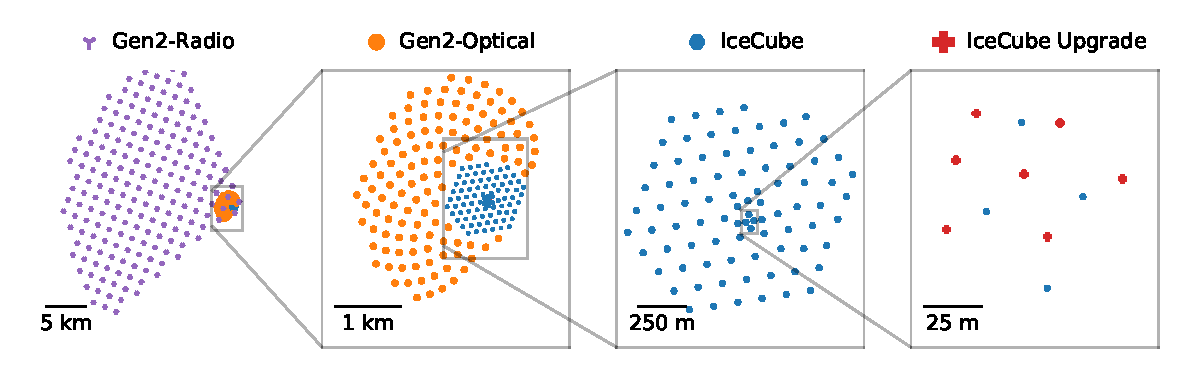
\includegraphics[scale=1.5]{./figures/gen2/decadal_survey_gen2-fan_radio_geometry.pdf}
	\caption[Layout of IceCube-Gen2 geometry]{Figure depicts the proposed IceCube-Gen2 Neutrino Observatory facility at the South Pole. It includes (from left to right) (i) a radio array with 200 stations, (ii) 120 new in-ice strings, spaced 240 m apart (shown as orange points), as an expansion of (iii) current optical array, (iv) 7 strings of IceCube upgrade, to be deployed soon within currrent in-ice DeepCore volume. Figure taken from \cite{whitepaper}}
	\labfig{gen2_all_geometry}
\end{figure}

\reffig{gen2_all_geometry} illustrates a top view of the IceCube-Gen2 facility, showcasing its various components using optimized technologies for the targeted energy ranges. 

\begin{description}
    \item \textbf{\emph{The IceCube Upgrade}} will start deployment this season (2024-2025 austral summer). Its goal is to lower the detection threshold for neutrinos to 1 GeV (In-line with its predecessor, \emph{DeepCore} in current IceCube)\sidecite{AYA}. This improvement will advance oscillation measurements, dark matter searches, and studies of physics beyond the Standard Model. The IceCube Upgrade project will also deploy 693 new multi-PMT detector modules on 7 new strings as shown in right-most panel of \reffig{gen2_all_geometry}, providing an opportunity to test the optical sensor technology for the IceCube-Gen2 observatory.

    \item \textbf{\emph{The Surface Array}} of IceCube-Gen2 is a setup of scintillator detector arrays on the surface of the South Pole, that measures the electromagnetic shower component and low-energy muons, while the optical array detects $\geq \mathrm{TeV}$ muons from the same air shower \sidecite{IceCubeCollaborationSchroeder2024_1000168735}. Planned to be used similarly as \emph{IceTop} of IceCube (see Section~\ref{sec:IC_detector}), the stations shall be placed on top of the additional \emph{in-ice} strings of optical array. It can also be used as \emph{surface veto} to reduce the background of atmospheric muons in samples of astrophysical neutrinos from the southern sky.

    \item \textbf{\emph{The Radio Array}} aims to discover and characterize the high-energy neutrino flux above 10 PeV. It detects nanosecond-scale radio emissions from ultra-high-energy particle showers using the Askaryan effect \sidecite{Askaryan,meyers_21}. This technique is sensitive to energies above a few PeV and complements the energy range of the optical array by capturing radio emissions from neutral and charged-current interactions, as well as energy losses of secondary leptons. The initial stations of the Radio Neutrino Observatory in Greenland, will serve as a R\&D tool for the Radio component of IceCube Gen2 \sidecite{rnog}.

    \item \textbf{\emph{The Optical Array}} The optical array will be expanded with the addition of 120 new strings to the existing IceCube strings. The strings will be arranged in what is referred to as "sunflower geometry," with an average horizontal spacing of 240 meters. The shape of the array and spacing between the strings will be determined through dedicated geometry optimization studies. Each string will contain 80 modules, resulting in a total of 9600 new modules. These modules will be placed between 1325 meters and 2575 meters below the surface, with a vertical spacing of 16 meters. This configuration will create an instrumented geometric volume of 7.9 cubic kilometers. The modules on the string are expected to collect nearly three times the number of photons gathered by an IceCube digital optical module (DOM) \sidecite{whitepaper}.
\end{description}

For the sensitivity study presented in this thesis, only the optical part of the proposed detector was simulated and used. 

\begin{figure}
	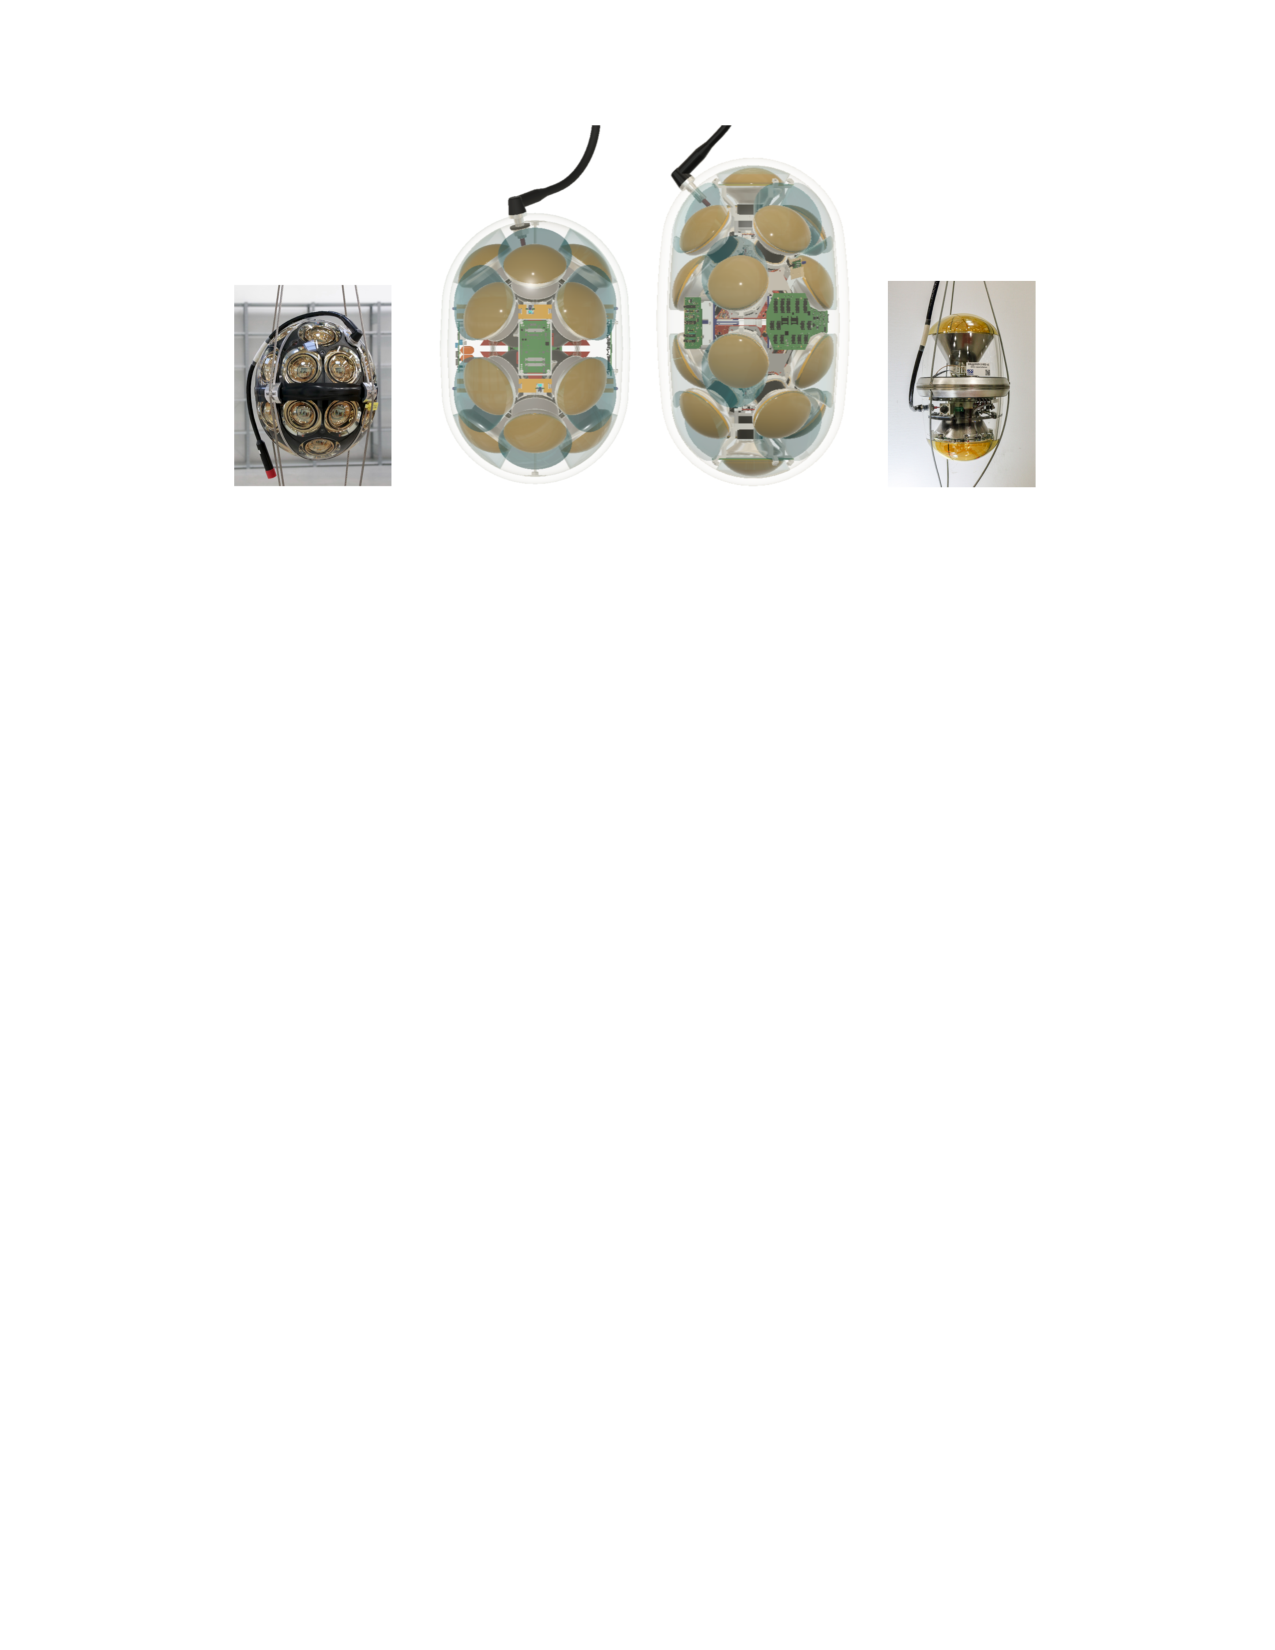
\includegraphics[scale=2.2]{./figures/gen2/Gen2_DOMs.pdf}
	\caption[Designs of candidate optical modules for IceCube-Gen2]{The designs of the IceCube-Gen2 optical sensors, DOM-16(second) and DOM-18 (third) with their base designs, to be used in the IceCube Upgrade sensors, are the mDOM on the left and D-Egg on the right \cite{Gen2_TDR}}
	\labfig{Gen2DOMs}
\end{figure}

\section{Simulation}
\label{sec:gen2-sim}
To perform this sensitivity study, dedicated simulations were carried out. The study aims not only to assess the sensitivity of IceCube-Gen2 for measuring the flavour composition of astrophysical neutrinos but also to evaluate its capabilities for detecting tau neutrino events, which is a crucial component as described in \refch{nu_samples}. The simulations were aligned with the mainline IceCube simulations (detailed in Section~\ref{sec:sim_ic}) to enable direct comparisons. However, necessary modifications were made to account for the new-generation optical sensors to be used in IceCube Gen2 and the sparser geometry. 

The following sections will describe the event samples created using these simulations to conduct the sensitivity analysis. First a brief overview of the \emph{simulated} sensor shall be given, where an isotropic sensor was created by assuming a spherical PMT, instead of a more realstic multi-PMT module, which requires considerable amount of time and resources to establish. The rest of the simulation chain remains identical to that explained in Section~\ref{sec:sim_ic} for mainline icecube simulations,
\begin{kaobox}
    particle generation $\rightarrow$ propgation of secondaries $\rightarrow$ photon propagation $\rightarrow$ Detector Simulation 
\end{kaobox}
Once the simulation is available, the selection cuts are applied to select only high energy events that starst within the detector volume, to mimic the so-called High Enegy Starting Event (HESE) described in Section~\ref{sec:HESE}. A classification of all HESE-like\sidenote{The selection is reffered as HESE-like and not exactly HESE as the original selection is sensitive to the detector geometry where outer layer DOMs are used as an active veto as described in Section~\ref{sec:HESE}. For this sensitivity
 study, an approximation was made by matching the effetive area of sample derived using IceCube-only strings.} events is then performed using a similar particle identifier described in Section~\ref{sec:PID} to classify these events in three morphologies, \textbf{Single Cascade,Double Cascades and Tracks}. 
\subsection{Isotropic Sensor}
\label{sec:isopdom}
The choice of optical sensors to be used in the IceCube-Gen2 project depends strongly on how well the reference optical sensors to be deployed in the IceCube upgrade perform.\sidecite{Gen2_TDR}. The designs have been carefully optimized to balance cost-effectiveness, logistical efficiency, and enhanced performance. \reffig{Gen2DOMs} shows both the 16 and 18 PMT modules, which are being considered to use in IceCube Gen2, along with \textbf{mDOM} (\emph{multi PMT Digital Optical Module}) \sidecite{mDOM_2017,mDOM_2019} and \textbf{D-Egg} (\emph{Dual optical sensors in an Ellipsoid Glass for Gen2}) \sidecite{D-Egg_MainPaper} that are to be deployed in ice for IceCube Upgrade.

\marginnote{\begin{kaobox}[title=pDOM]
    pDOM stands for PINGU Digital Optical Module. It was first coined for an R\&D upgrade of IceCube DeepCore called \textbf{PINGU} (The Precision IceCube Next Generation Upgrade) \cite{PINGU}.
\end{kaobox}}

The maturity of the design, along with extensive in-situ testing using a large number of sensors for the IceCube Upgrade, leads us to consider the mDOM-type sensor as the baseline for evaluating the IceCube Gen2 detector's capabilities in identifying Tau neutrino-induced Double Cascade events. Unlike IceCube’s single large 10" PMT, the mDOM consists of 24 smaller 3" PMTs. The key advantages of the mDOM over pDOM \sidecite{PINGU} are its 2.2 times higher effective photocathode area, omnidirectional sensitivity, and the directional information obtained from the individual “pixels” (the 24 PMTs). Due to the large number of PMTs and their strategic placement within the module sphere, this module offers nearly isotropic angular acceptance, unlike IceCube DOMs with only one downward-facing PMT. 

The effective area of the optical modules is the equivalent physical cross-section that would detect all the incident photons from a plane perpendicular to a given direction. As illustrated in \reffig{EffectiveArea_mDOM} (Left plot), the mDOM has a nearly constant effective area for collecting photons from all directions, unlike the Gen1 DOMs (pDOMs) which have a downward-facing PMT. As a result, the effective area for pDOMs increases as the arrival direction shifts from 180 degrees ("down-going" in the IceCube coordinate system) to 0 degrees ("up-going" in the IceCube coordinate system).

\begin{figure}
    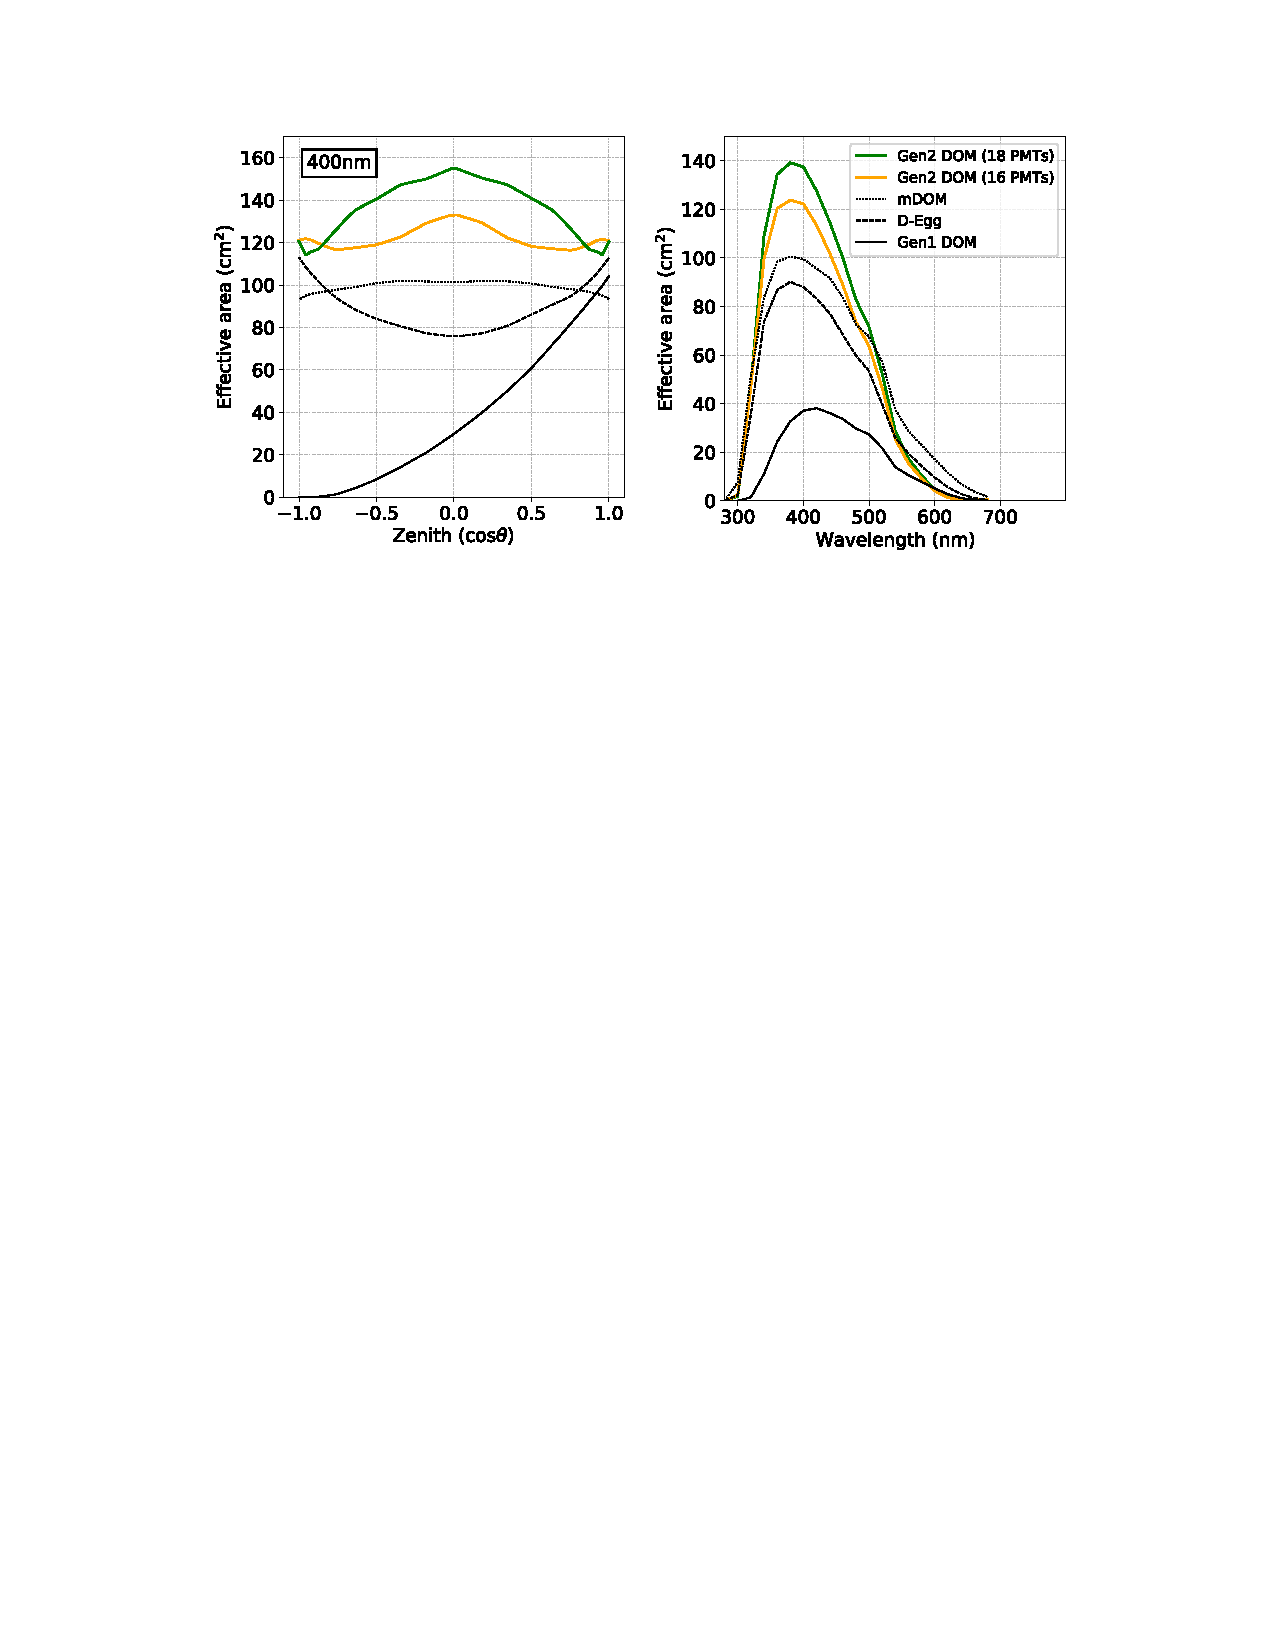
\includegraphics{./figures/gen2/EffectiveAreaCurve_TDR.pdf}
    \caption[DOM effective area comparisons of Multi-PMT modules with a current single PMT DOM of IceCube]{The effective area is compared for IceCube-Gen2 DOM candidates, 16, and 18 PMT models, in relation to IceCube-Gen1 DOM (pDOM), D-Egg, and mDOM, as functions of zenith angle (left) and wavelength averaged over solid angle (right). Figure taken from \cite{Gen2_TDR}} 
    \labfig{EffectiveArea_mDOM}
\end{figure}

However, current simulation methods used in IceCube (see Section~\ref{sec:mc_sim}) do not yet provide a detailed simulation of a multi-PMT module, so a simulated sensor called \emph{iso-pDOM} (isotropic-pDOM) was developed \sidecite{Anastasiia_Thesis}. This sensor can be thought of as a 'spherical PMT' encased in a glass vessel similar to an IceCube DOM but with 2.2 times higher quantum efficiency, capable of capturing photons arriving from all the directions (see \reffig{isoPDOM_schematic}). The sphere was simulated by assuming an upward-facing PMT along with a downward one and combining the results while maintaining the same area under the curves at all wavelengths. The resultant iso-pDOM has an effective area very similar to that of an mDOM.

\begin{marginfigure}
    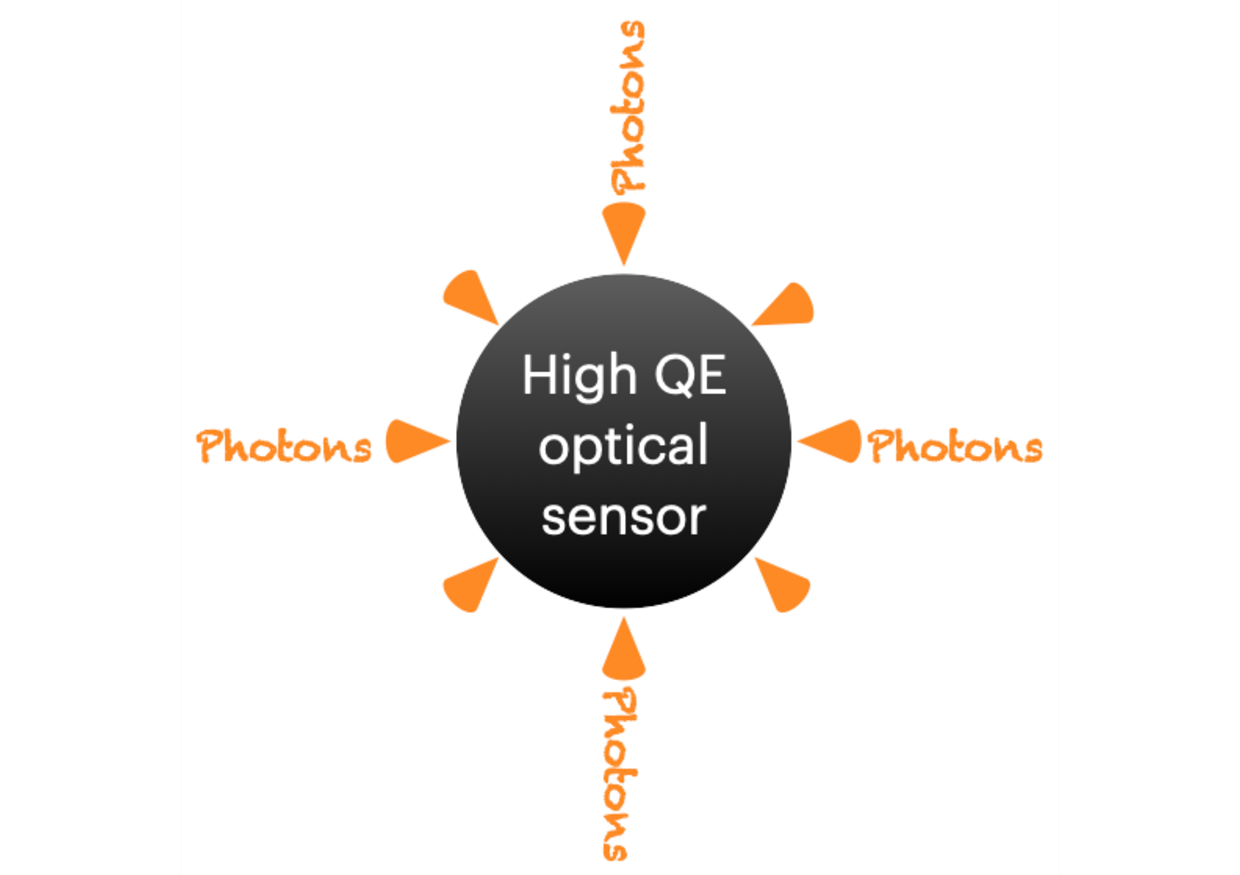
\includegraphics{./figures/gen2/iso-pDOM.pdf}
    \caption[Schematic of an isoPDOM]{Conceptual representation of Simulated sensor with isotropic angular acceptance (iso-pDOM)}
    \labfig{isoPDOM_schematic}
\end{marginfigure}

\begin{figure}
    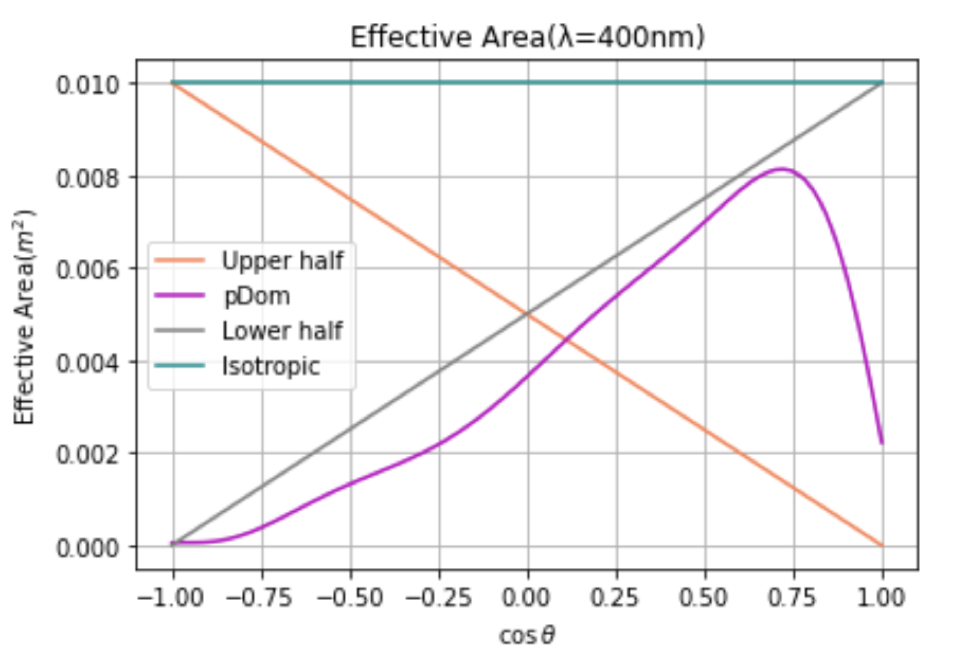
\includegraphics{./figures/gen2/isopDOM_eff_area.png}
    \caption[Effective area of isoPDOM]{Results of simulating a sensor that \emph{mimics} the behaviour of a typical mDOM. The blue line shows changed effective area of the so-called \emph{isopDOM}, achieved by combining acceptance curves of pDOMs having a PMT in "upper" (orange) and "lower" (grey) halves of the DOM respectively}
    \labfig{isoPDOM_effarea}
\end{figure}


\subsection{Event Selection}
\label{sec:gen2_eventsample}

Monte Carlo events were produced using isoPDOM for all three flavours of primary neutrinos with energies ranging from 100 TeV to 50 PeV. The simulation chain is identical to that described in Section~\ref{sec:mc_sim}. It is important to note that since the IceCube in-ice array is inherently part of the proposed Gen2 detector, all simulated events still include information (collected charge) collected by IceCube DOMs from the IC86\sidenote{IC86 stands for the current IceCube detcetor volume, made up of 86 strings containing Digital Optical Modules (DOM).} configuration. Additionally, during the Detector Simulation stage of the simulation chain (see Section~\ref{sec:mc_sim}), where PMT responses, noise, etc., are added, responses are incorporated separately for IceCube DOMs and isoPDOMs. If an event passes all the basic triggers, two separate triggers are stored depending on the event location: IC86 and ICGen2. By default, ICGen2 has a combined response of both detector configurations, while IC86 only contains current IceCube volume events. This feature is crucial as it facilitates direct comparison of events produced with IceCube simulations for IceCube-only analyses.

A fundamental aspect of flavour measurement studies is the ability to identify the flavour of the neutrino involved in an interaction. This identification is possible due to the distinct by-products produced by different neutrino interactions, which result in unique light deposition patterns, or "morphologies" as described in Section~\ref{sec:morphologies}. These patterns, illustrated in \reffig{topologies}, allow us to reconstruct the events by analyzing the pattern of photon detections in the detector. By doing so, the flavour of the original interacting neutrino can be determined.

To utilize the same particle identifier used in the analysis preseneted in \refch{analysis} for this sensitivity study, a dedicated event selection process for high-energy starting events (HESE) \sidecite{HESE7_sample} was implemented. However, since the outer-layer detector veto is specific to the detector geometry and the characteristics of the DOM pulses—which is still under development for the IceCube-Gen2 simulation chain-starting events were selected by examining the interaction vertex of the primary neutrino. This interaction vertex was further refined by considering the deposited charge (measured in single photoelectrons) and calculating the charge-weighted mean positions. This charge information is crucial for applying a HESE-like charge cut. Unlike the 6000 photoelectrons threshold used previously, the threshold for this analysis was set at 2000 photoelectrons. The lower threshold is due to the higher quantum efficiency and isotropic sensitivity of the new sensors, which enhance the detection capability for high-energy events. All the approximations made were in parallel checked for IC86 configuration to reproduce Monte Carlo PDFs within statstical erros to the ones presented in analysis chapter.

Moreover, to appropriately weight the simulated events and account for the probability of an atmospheric neutrino being rejected by an accompanying muon triggering the veto, a dedicated calculation similar to the one used in the HESE-7.5 analysis \sidecite{HESE7_sample} was used. Additionally, the reconstructed energy cut, initially set at 60 TeV, was adjusted to 100 TeV. This adjustment was based on the signal-to-background probability density functions (see \reffig{DC_PDFs}) to ensure a similar signal-to-background ratio (2:1) as achieved in the HESE-7.5 analysis \sidecite{Juliana_paper} and the HESE-12 analysis, presented in \refch{analysis} and \refch{HESE12}. A peculiar observation while looking at Monte Carlo PDFs shown in \reffig{DC_PDFs} compared to those shown in \reffig{LvsE_signalbkg} can be seen due to limited number of produced Monte Carlo for this study. Although, even with low stastics, more population along the LvsE diagonal is clearly visible on the left panel showing signal Double Cascade events. 

After applying all the necessary filters, the final sample includes starting events with a reconstructed deposit energy of 100 TeV or more and a charge exceeding 2000 PE. These events originate from interactions of all six types of neutrinos (particle and antiparticle versions of 3 flavours) beginning within the simulated IceCube-Gen2 fiducial volume. They are divided into three categories: Tracks, Single Cascades, and Double Cascades.

\begin{figure*}[h]
    \begin{subfigure}[h]{0.7\textwidth}
        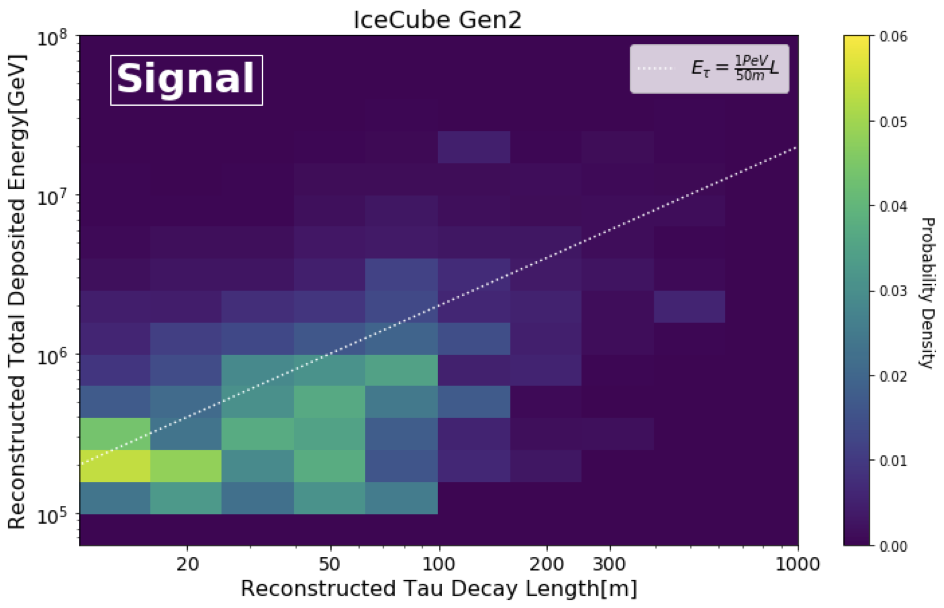
\includegraphics{./figures/gen2/Signal_PDF.png}
    \end{subfigure}
    \hfill
    \begin{subfigure}[h]{0.7\textwidth}
        \includegraphics{./figures/gen2/Bkg_PDF.png}
       
    \end{subfigure}
    \caption[2D Monte Carlo PDFs of reconstruct energy and length for double cascade events in IceCube-Gen2]{Two dimensional Monte Carlo templates, constructed using reconstructed total energy ($E_{\text{Tot}}$) and double cascade length ($L_{\text{dc}}$) for events classified as \textbf{double cascades}. The signal (left), representing $\nu_\tau$-induced double cascades, shows a clear correlation between $L_{\text{dc}}$ and $E_{\text{tot}}$. In contrast, the background (right), consisting of $\nu_\mu$ and $\nu_e$ events, lacks this correlation and clusters at low $L_{\text{dc}}$.}
    \labfig{DC_PDFs}
    
\end{figure*}


\section{Analysis tool : \texttt{toise}}
\label{sec:toise}
Understanding and enhancing the sensitivity of the detector can result in more precise and dependable performance, thus improving the scientific impact of the experiment. The main goal of the sensitivity studies carried out in this work is to optimize the design of the detector in order to be capable of reconstructing tau neutrino events using existing methods, but with a larger detection volume and new generation optical sensors. Additionally, one can also assess the sensitivity of the detector by combining both radio and optical arrays of the proposed detector to investigate flavour measurements in the energy ranges from TeV to EeV \sidecite{Coleman}.

It's impractical to run comprehensive simulations for evolving detector designs due to the large amount of computing power required. The \texttt{toise} \sidecite{toise} framework was created to estimate sensitivity using a simplified model of the detector response based on targeted Monte Carlo (MC) simulations. This allows for efficient comparisons of different detector designs without repeating the entire simulation process. \texttt{toise} was used for a sensitivity study presented in the next section. This section will provide a brief overview of its workflow. In order to distinguish the influence of design choices on detector performance from the intrinsic restrictions imposed by neutrino interaction physics, the event rate calculation in this framework is conducted through two distinct stages: Neutrino Physics and Detection.

In the Physics stage, the neutrino fluxes at the Earth's surface are converted to the detector's area or volume. This involves using a transfer tensor to model the conversion between the initial neutrino flavour states and the observable final states (muons, hadrons, etc.). In addition, various aspects of neutrino interactions, including neutrino-nucleon cross-sections and different interaction types (neutral current or charged current) are also taken into account. The transfer tensor is subsequently combined with the final-state effective area to establish a neutrino effective area. The effective area \( A_{\text{eff}}(E, \theta) \) of the detector is calculated by multiplying the geometric area \( A_{\text{geo}}(\theta) \) with an energy and zenith-dependent efficiency \( \eta(E, \theta) \):

\begin{equation}
    A_{\text{eff}}(E, \theta) = A_{\text{geo}}(\theta) \times \eta(E, \theta)
\end{equation}

For the optical array of the proposed IceCube-Gen2, the geometric area is approximately calculated by placing a convex hull around the instrument's geometric boundary. \textbf{\emph{The selection efficiency}} \( \eta(E, \theta) \) characterizes the detector's triggering efficiency and the probability of an event passing a set of analysis criteria. It is defined as \emph{the ratio of events passing these cuts to the number of events generated}. Depending on the type of sensitivity study being performed—such as expected limits, discovery potential, or flavour measurement—additional parameterizations like energy and angular resolutions and classification efficiency are used. For flavour measurement, \textbf{\emph{the classification efficiency}} generates an event classification smearing matrix (\reffig{classeff}) and is defined as \emph{the fraction of morphology per energy bin for a given neutrino flavour}.

When estimating sensitivities, it is essential to account for backgrounds that may mimic the signal. The framework handles backgrounds by either adding their contributions to the event rate or ignoring regions where they are expected to contribute. For all detectors and science cases, atmospheric neutrino flux is added as a background using the same effective area as for astrophysical neutrinos. Optionally, atmospheric neutrino flux in the downward-going region can be reduced to account for vetoing by accompanying muons from the same air shower. This is done in a similar way to the one described in Section~\ref{sec:selfveto}.

\section{Result of Flavour Sensitivity Measurements}
\label{sec:gen2-results}
Using the HESE-like sample, described in Section~\ref{sec:gen2_eventsample}, a detector response tensor is generated using \texttt{toise}. Selection efficiency, detailed in Section~\ref{sec:toise}, is a key factor in generating the detector's neutrino effective area. This efficiency is determined using \reffig{selecteff}, which shows the true deposited energy at which the analysis starts to select events. The plot illustrates the ratio of events passing all selection cuts in Section~\ref{sec:gen2_eventsample} to all simulated neutrinos reaching the fiducial volume, per energy bin. The curve is fitted, and the resultant plot shows that neutrinos are selected starting from approximately 200 TeV. This value is used as the selection threshold for events beginning or contained in the fiducial volume.

\begin{figure}[h!]
    \centering
      \includegraphics{./figures/gen2/SelectionEff.pdf}
      \caption[Selection Efficiency of HESE-like selection in IceCube-Gen2]{Selection Efficiency : Ratio of neutrinos that got classified into a morphology to all the neutrinos that interacted in active volume. Data here refers to monte-carlo events per energy bin.}
  \labfig{selecteff}
  \end{figure}


A specific parameterized tensor is used to determine the efficiency of particle identification during flavour measurements. \reffig{classeff} shows how well the reconstruction process can identify different types of particles based on their morphologies. In an ideal scenario, events involving charged current interactions with electron neutrinos ($\nu_e$) are classified as single cascades, those involving muon neutrinos ($\nu_{\mu}$) as tracks, and those involving tau neutrinos ($\nu_{\tau}$) as double cascades. The diagonal elements of the plot show how accurate the classifier is, while the off-diagonal elements indicate the fractions of misidentified flavours. The plot shows that as the true deposited energy increases, the number of double cascade events (from $\nu_{\tau}$ interactions) initially plateaus and then decreases. This occurs because at higher energies, the individual energy depositions are further apart (due to correlation of $\mathrm{L}_{\mathrm{dc}}$ and $\mathrm{E}_{\mathrm{tot}}$), making it easier for the reconstruction process to distinguish them. However, at even higher energies, one of the cascades may be partially or completely outside the detector, causing these events to be misclassified as single cascades due to strict containment criteria, as described in Section~\ref{sec:PID}. For single cascades involving $\nu_e$, the efficiency decreases at high energies because some DOMs may become saturated, and their data is excluded from the analysis. In contrast, the efficiency for starting tracks remains relatively consistent across the entire energy range.


\begin{figure}[h!]

    \centering
    \includegraphics{./figures/gen2/ClassificationEff_small_watermark.pdf}
    \caption[Classification efficiency of a ternary particle identifier for IceCube-Gen2]{Classification Efficiency: Three subplot columns are true neutrino flavours, where each energy bin (true Monte Carlo energy) contains the fraction of topologies, summing to 100\%. Diagonal plots show the flavour identification efficiency of the classifier, whereas off-diagonal plots show misidentification fractions.
    }
    \labfig{classeff}
\end{figure}

Lastly, a significant advantage of \texttt{toise} is its ability to combine different event selections and detector types. The starting event sample from this detailed study can be combined with the efficiencies of other samples, such as through going tracks sample. In \texttt{toise}, these efficiencies are included by limits derived from IceCube analysis \sidecite[-2cm]{diffusenumu} to calculate angular resolutions, PSF, etc. The flavour measurement presented here demonstrates the sensitivity of IceCube Gen2 by combining starting events with through-going muons, a method already realized in IceCube \sidecite[-2cm]{Neha_ICRC_IC}.

\reffig{Gen2_flavourtriangle} shows the projected flavour measurement sensitivity of IceCube-Gen2 with 10 years of data \sidecite{Neha_ICRC_Gen2}. It is derived by using an asimov dataset \sidecite{asimov} assumes equal partition of all flavours, with a diffuse neutrino spectrum following a single power-law with an index of 2.5 and a per-flavour normalization of 2.3 \sidecite{lars_globalfit}. The confidence intervals are derived by assuming wilks' theorem \sidecite{Wilks_thm}, as for analysis presented in \refch{HESE12}. The figure also illustrates the sensitivity change if a dedicated $\nu_{\tau}$ identifier is not included in the starting event sample, resulting in the sample containing only single cascades and tracks, making it impossible to resolve the $\nu_e$ and $\nu_{\tau}$ fraction degeneracy. The systematic variations arising due to detector are neglected. 

\begin{figure}[h!]
    
    \caption[Sensitivity of IceCube-Gen2 to measure flavour composition of Astrophysical neutrino with 10 years of its lifetime]{Projected sensitivity of IceCube-Gen2 to measure flavour composition of Astrophysical neutrino with 10 years of its lifetime. The maroon line shows sensitivity using the ternary classification scheme and light salmon shade shows sensitivity \textbf{without} a dedicated $\nu_{\tau}$ identifier. The unresolved degeneracy along $\nu_e$/$\nu_{\tau}$ axis is notable due to lack of double cascade classifier. The solid (dashed) lines depict the corresponding 68\% (99\%) constraints, derived assuming Wilks' theorem.}
    \includegraphics{./figures/gen2/Gen2-10Years.pdf}
    
    \labfig{Gen2_flavourtriangle}
\end{figure}

The sensitivity shown in \reffig{Gen2_flavourtriangle} and applies to the entire diffuse neutrino spectrum. With this study, flavour measurement for a given 'slice' of energy was also done to characterize its energy dependence. As described in Section~\ref{sec:astro_nu}, diffuse neutrino spectrum consists of neutrinos originating from various high-energy sources in all directions. Depending on the environments of the acceleration sites (magnetic fields, accretion disks, dust, etc.), the production ratios of neutrinos at the sites may differ \sidecite{cite166}. The most commonly assumed model, is the pion decay scenario (see Section~\ref{sec:flavour_theory}). At higher energies, however, due to synchrotron cooling of secondary muons produced in pion decay (see Equation~\ref{eq:pipm_decay}) the flavour production at sources changes to a ratio of ($\nu_e:\nu_{\mu}:\nu_{\tau}$) from 1:2:0 to 0:1:0 \sidecite{walter_muondamped}. If such sources begins to dominate the overall flux at high energies, a transition in measured neutrino flavour fluxes can be observed \sidecite{muon_damp}. \reffig{gen2_muondamped} shows IceCube-Gen2's sensitivity to detecting such a flavour transition. The assumed "critical energy" for this mechanism for the study is 2 PeV. This transition is detectable with IceCube-Gen2 due to its extended energy range, enabled by its approximately eightfold increase in volume \sidecite{Gen2_TDR}.

\begin{figure}[h!]
\centering
    \includegraphics{./figures/gen2/MuonDamped.pdf}
    \caption[Sensitivity of IceCube-Gen2 to measure an energy dependent flavour composition of Astrophysical neutrino]{The bottom section displays the proportion of $\nu_{\mu}$ at the source based on energy, with the assumption that the muon critical energy is 2 PeV. The error bars represent the 68\% confidence level limitations on the $\nu_{\mu}$ fraction below and above 1 PeV, derived from the observed flavour composition of $\nu_{\mu}$ at Earth using IceCube-Gen2 and assuming standard oscillations. In the upper sections, the dark (light) shaded regions depict the corresponding 68\% (99\%) constraints, without making any assumptions about the mixing matrix.}
    \labfig{gen2_muondamped}
\end{figure}

The power of combining different event samples, extension of detector volume along with an isotropic module already shows a significant gain in sensitivity to measure flavour composition of astrophysical neutrinos. Furthermore, the optical component of IceCube Gen2 will also be sensitive to detect a changing flavour composition as a function of neutrino energy, that shall allow us to distinguish population of dominating sources across the spectrum. The study presented above can be further extended by adding the proposed radio component to the sample \sidecite{Coleman}. As described in Section~\ref{sec:gen2-detector}, due to the extended radio array IceCube-Gen2 shall be sensitive to measure EeV neutrinos as well \sidecite{Gen2_TDR}. \reffig{gen2_radioincluded_flavour} shows extension of sensitivity projection shown in \reffig{gen2_muondamped}, by adding flavour tagging at higher energies. It shows that at even higher energies, where the diffuse neutrino spectrum is dominated by cosmogenic neutrinos (see Section~\ref{sec:cosmogenic_nu}), the measure flavour ratio transitions back to the 1:2:0 scenario at the source \cite{Coleman}.  


\begin{figure*}[h!]
    \centering
        \includegraphics{./figures/gen2/energy_dependence_Gen2_TA-GZK.pdf}
        \caption[A combined sensitivity of IceCube-Gen2 to measure flavour composition of Astrophysical neutrino using both optical and radio components of the detector]{A combined sensitivity to measure evolution of the neutrino flavour composition with energy ranges from TeV to EeV range, using both optical and radio components of IceCube Gen2 Detector. Astrophysical neutrino sources are generally expected to be dominated by pion decay at the lowest energies, with a flavour composition of approximately (1:2:0). At intermediate energies, the sources transition to a muon-damped production regime, yielding a flavour ratio of roughly (0:1:0). Finally, at the highest energies, the composition reverts to the pion decay pattern, (1:1:1), as anticipated for cosmogenic neutrino production. The details for layout are similar to that shown in \reffig{gen2_muondamped}. The extended figure, taken from \cite{Coleman}.}
        \labfig{gen2_radioincluded_flavour}
    \end{figure*}

To conclude, IceCube-Gen2's increased volume will improve the detection rate of tau neutrinos, which are identifiable by their unique "double-bang" decay signature. This enhancement in tau neutrino identification, especially above 300 TeV, will provide critical insights into the flavour composition of astrophysical neutrinos, enabling stronger constraints on source physics and the potential to detect new physics beyond the Standard Model. Furthermore, the inclusion of a radio array may extend tau neutrino detection capabilities to even higher energies in the EeV range, offering unprecedented precision in exploring the universe's most extreme neutrino sources. The enhanced sensitivity of IceCube-Gen2, achieved through the combination of optical and radio detection methods, will close critical gaps in our understanding of the cosmic neutrino energy spectrum, extending the detection range up to three orders of magnitude higher than current capabilities. This leap in sensitivity will enable the discovery of ultra-high-energy neutrinos, paving the way for transformative progress in both high-energy physics and astrophysics. 
% \setchapterpreamble[u]{\margintoc}
\chapter{Summary and Outlook}
\labch{summary}

The aim of this thesis was to measure the flavor composition of astrophysical neutrinos using the High Energy Starting Event (HESE) sample, collected over approximately 12 years. This analysis involved classifying HESE events into three morphological categories: single cascades, tracks, and double cascades. Each morphology typically correlates with a unique neutrino flavor interaction, so this classifier, known as a particle identifier or ternary classifier, is useful for distinguishing neutrino types. Appropriate variables were selected to build Monte Carlo probability density functions (PDFs) that effectively differentiate signal from background events. For electron and muon neutrinos ($\nu_e$ and $\nu_\mu$), single cascades and tracks were analyzed against atmospheric neutrino backgrounds, whereas tau neutrino ($\nu_\tau$) backgrounds predominantly originated from other flavor misclassifications. A likelihood fit was then applied to events with reconstructed energies above 60 TeV.

In the double cascade topology, events arising from $\nu_\tau$ charged-current (CC) interactions exhibit a relationship between the reconstructed total energy deposited and the length of the reconstructed double cascade. This feature is absent in misclassified neutral-current, $\nu_e$-CC, and $\nu_\mu$-CC events. This unique topology, resolvable at high energies, helps break the $\nu_e$-$\nu_\tau$ degeneracy at energies above $\sim 100$ TeV, thereby improving direct sensitivity to each flavor in combination with single-cascade and track topologies. The work in this thesis focused on three main parts: updating the ternary classifier with recent ice models, reconstruction tables, and simulations; performing a likelihood fit to measure the flavor composition using an additional four years of HESE data compared to prior studies; and producing Monte Carlo simulations targeted at the future IceCube-Gen2 detector to extend the classifier to the next-generation detector.

The classifier update was comprehensive, entailing adjustments to the neutrino weight in the sample, which influences expected event rates and Monte Carlo PDFs for reconstructed quantities. This included a new classification to reduce background events from high-energy $\nu_e$ single cascades near the Glashow resonance, alongside corrections for assumed neutrino interaction cross-sections in Glashow events. Adjustments to the CC tau neutrino events were also made to account for the polarized states of tau leptons, affecting the energy distribution of decay products, an important variable in double-cascade reconstruction. Though no significant differences were observed at the analysis level, these corrections were retained.

Further, updates incorporated a refined ice model, SPICE-Bfr, for reconstruction. Because the reconstruction method relies on tabulated light yield—generated with a specific ice model—and the double-cascade length reconstruction is particularly sensitive to ice anisotropies, the new model was used as it aligns best with current data. Additionally, a novel simulation technique called the SnowStorm technique was applied, where detector systematics varied continuously rather than requiring discrete Monte Carlo sets.

In performing the likelihood fit, parameters and flux components were updated from prior iterations. For uncertainties in detector systematics, the Snowstorm approach was used, where detector parameters vary continuously to capture systematic uncertainties. While many other parameters affecting cosmic-ray spectrum features were included, they had limited impact on the fit. A key addition was the inelasticity parameter, which influences the energy deposition and thereby normalizes the observed spectra. Updated software was also employed in this analysis.

In applying the first two steps of the updated methodology, the 7.5-year dataset saw an unexpected surplus of double-cascade events compared to previous data unblindings. Investigation revealed this excess was likely due to incorporating the high-quantum-efficiency DeepCore DOMs in the reconstruction, which hadn’t been done previously. However, the simulation predictions did not match the observed data. A deeper investogation discovered a bug in the charge template used in data calibration files. The data files used older template while simulation had been updated with the new ones. This inconsistency between simulation and data was problematic for maximum-likelihood energy estimation methods that rely on charge templates. Ultimately, DeepCore DOMs were removed from the reconstruction, and the likelihood fit was re-performed, leading to a final 12-year dataset with 5 double cascades, 64 single cascades, and 28 track events above 60 TeV. The resulting best-fit flavor composition was $\nu_e : \nu_\mu : \nu_\tau=0.19:0.43:0.38$, consistent with previous measurements, indicating a preference for a muon-damped source scenario but insufficient sensitivity to reject alternative models such as the no-astrophysical $\nu_\tau$ hypothesis at even a $1\sigma$ level, though designed for $2\sigma$ sensitivity. Monte Carlo pseudo-experiments demonstrated that many observed events fall in bins where the signal-to-background ratio is low, hampering the fit’s ability to distinguish signal from background effectively.

The analysis in this thesis underscores the challenges posed by limited statistics in the HESE sample for flavor composition measurements. The low number of double-cascade events constrains the statistical power, which could be significantly improved by including additional high-statistics samples, particularly cascades and tracks, to better constrain $\nu_e$ and $\nu_\mu$ fractions. The findings suggest that the classifier and the analysis method could benefit from revisions before future fits, given the sensitivity of the double-cascade reconstruction to minor methodological changes. For instance, while double-cascade events like \textbf{Double Double} remain consistently classified in every configurations (and even analyses, including the one presented here and both \sidecite{Juliana_paper,CNN_tau} ), the inclusion or exclusion of DeepCore DOMs and slight changes in ice models cause notable classification shifts, questioning the classifier's robustness. The cut values used to separate signal from background were initially derived assuming a harder neutrino flux spectrum, where more high-energy events would increase $\nu_\tau$ counts \sidecite{marcel_thesis}. Since the HESE spectrum is softer, these cut values should be re-evaluated to enhance sample purity. The simulations were generated with an older ice model version, which further impacts data-mc agreement and could improve the results if updated. Although the analysis did not yield a groundbreaking measurement, it illuminated critical issues with the reconstruction methods, suggesting areas for improvement in future studies. 

\begin{figure}[h]
    
    \includegraphics{./figures/results/3D_Combined.png}


    \caption{The sensitivity to measure flavor composition by combining 12 years of HESE sample with current GlobalFit sample \cite{globalfit_icrc}, for an astrophysical neutrino spectrum following the single unbroken power-law given as $E^{-2.3}$, with a flavor composition of $\nu_e : \nu_\mu : \nu_\tau = 1 : 1 : 1$.
    }
    \labfig{globalfit}
\end{figure}

A combined global fit using multiple samples could offer stronger constraints on flavor ratios in future analyses. As shown in \reffig{globalfit} in projected sensitivity, adding 12 years of HESE data to a recently unblinded global fit\sidenote{Note that the figure is produced assuming a single power law of index 2.3, and not the broken power law result of the globalfit \cite{globalfit_icrc}} could provide around $3\sigma$ sensitivity to rule out models like the neutron-beam scenario, assuming an equitable flavor partition. Additionally, exploring alternative detection techniques, such as convolutional neural networks (CNNs) for double-pulse signature recognition, could aid in $\nu_\tau$ detection, especially for lower-energy events. This double-pulse technique—analogous to double-cascade identification—could expand analysis to events up to a few hundred TeV, where pulses on DOMs are sufficiently close to register as two distinct signals. This method is already used within IceCube \cite{CNN_tau}, providing a foundation for future $\nu_\tau$ detection efforts.

As highlighted, precise knowledge of the ice model is essential for reconstruction accuracy. IceCube's Upgrade project will place new calibration devices with improved resolution to map Antarctic ice properties, enhancing the accuracy of double-cascade length resolution and advancing oscillation studies across a wide energy range \sidecite{AYA}. Future improvements in ice optical property data from these upgrades will support higher fidelity in simulations and more consistent agreement with observed data, which is vital for tau neutrino detection. The larger-scale IceCube-Gen2 project will open even greater possibilities with its 8-fold volume increase and improved PMT modules, expanding sensitivity for astrophysical neutrino detection across broader energy scales.  IceCube-Gen2 will also support more accurate cascade angular reconstruction, which will aid in $\nu_\tau$ identification and benefit follow-up observations with electromagnetic telescopes due to the relatively low atmospheric background in $\nu_\tau$ signals. This expanded scope could even facilitate identification of changes in neutrino production scenarios at different energy levels, potentially revealing dominant source classes at specific energy thresholds. By combining optical and radio arrays, Gen2 could reach energies accessible to cosmogenic neutrinos, which are otherwise limited by the GZK cutoff in cosmic-ray studies. The new optical sensors and improved angular resolution in double-cascade detection will not only enhance $\nu_\tau$ identification but may also offer a nearly background-free signal, providing invaluable data for locating and studying astrophysical neutrino sources.



\cleardoublepage

\appendix
\pagelayout{wide}
\addpart{Appendix}
\pagelayout{margin}
% \setchapterstyle{lines}
\chapter{Mean SPE Charge Distribution of DOMs}
\label{ch:spe_check}
One of the stages of the unblinding stage of the analysis presneted in \refch{HESE12} involved a strong Data-Monte Carlo disagreement between obsreved and expected number of Doubel Cascade events when DeepCore DOMs were included in the analysis. While DeepCore DOMs have been excluded from the previous iterations of this analysis \sidecite{Juliana_thesis,marcel_thesis} due to the bias they bring to \texttt{millipede} based reconstructions used in this analysis (see Section~\ref{sec:reco}), recent modifications in the simulations made it possible to use them again. Nevertheless, the access of observed double cascade events in 7.5 years of HESE data, initiated a series of detailed checks to understand the root of the problem, \emph{Why is inclusion of the  DeepCore DOMs causing a Data/Monte Carlo mismatch?}. The following section describes some issues observed in regards to single photoelctron (spe) charge templates used in simulation and data, that are used in \texttt{millipede} to calculate the observed light yield of the event. This work was done in collaboration with Jakob Van Santen\footnote{DESY - Deutsches Elektronen-Synchrotron
Platanenallee 6, D-15738, Zeuthen

email : jakob.van.santen@desy.de}.

In the Monte Carlo processing chain described in Section~\ref{sec:mc_sim}, at the Detetcor Simulation stage, the acceptance of a photon arriving at a Digital Optical Module (DOM) and the charge assigned to it are determined by several key factors. The acceptance is influenced by the global DOM efficiency, which scales the overall probability of photon detection, as well as the relative DOM efficiency, which accounts for variations in performance among individual DOMs. Additionally, angular acceptance curves are employed, which consider the interaction location and the angle of the photon relative to the DOM surface. This multi-faceted approach ensures a more accurate representation of the photon acceptance process.
\sidenote{\begin{kaobox}
    Note that High QE DeepCore DOMs exhibit a distinctly different shape compared to  non-DeepCore DOMs, leading to a mean charge that is 3.6\% lower than that of NQE DOMs. To account for this difference, the compensation factor is adjusted to be 3.6\% higher (effectively resulting in a 3.6\% higher Relative DOM Efficiency, or RDE), ensuring that the total charge collected remains consistent following the implementation of the SPE Templates.
\end{kaobox}}
To enhance the charge assignment, the new Single PhotoElectron (SPE) Templates (right panel of \reffig{SPE_oldnew}) have replaced the previous method (left panel of \reffig{SPE_oldnew}) of sampling from the general TA0003 charge distribution \sidecite{SPE_paper}. Each DOM now features a uniquely measured in-ice charge distribution, which is stored in the Geometry, Calibration, and Detector (GCD) file. This distribution is characterized by the sum of two exponential functions and a Gaussian, accurately reflecting the single-photoelectron response. Furthermore, the SPE Templates incorporate a global residual correction, a DOM efficiency scaling factor, and a charge scaling factor to account for shifts observed between processing passes. This comprehensive methodology enables the DOM Launcher to assign a charge that more accurately represents each DOM's behavior in the detector simulation.

\begin{figure*}[h!]
    \begin{subfigure}[h]{0.7\textwidth}
        \includegraphics{./figures/results/Old.pdf}
    \end{subfigure}
    \hfill
    \begin{subfigure}[h]{0.7\textwidth}
        \includegraphics{./figures/results/simulation.pdf}
    \end{subfigure}
    
    \caption{Distribution of the Single Photoelectron (spe) charge distribution for DOMs, shown separately for High Quantum Efficiency DeepCOre DOMs (blue) and for rest of the DOMs (orange). The vertical line shows the average SPE charge per DOM, after applying the compensation factor. Left Panel shows the old distribution, and right panel shows the updated distribution.}
    \labfig{SPE_oldnew}
\end{figure*}

While this update has been implemented in the simulation used for the analysis presented in this thesis, which employs the updated Single PhotoElectron (SPE) template (see \reffig{SPE_sim}), the corresponding data files were not updated with this new parameterization until 2023. The Data GCD files still contained the parameterization based on the old template, as illustrated in the left panel of \reffig{SPE_oldnew}. The figures show the distribution of mean SPE charge for both DeepCore and Non-DeepCore DOMs. Notably, the old template reveals a significantly larger deviation (greater than 10\%) for DeepCore DOMs compared to Non-DeepCore DOMs, which display only about a 5\% deviation. This occurs against a backdrop where the mean SPE charge is approximately 0.85, where we define 1 PE as the mean of the Gaussian component of the SPE charge distribution. It’s important to note that while this value represents 1 PE, the distribution is not purely Gaussian and includes a population below the valley, leading to an average value of less than 1.
\begin{marginfigure}
    
    \includegraphics{./figures/results/Updated.pdf}


    \caption{Distribution of the Single Photoelectron (spe) charge distribution for DOMs used in Simulation. See caption of \reffig{SPE_oldnew} for details.}
    \labfig{SPE_sim}
\end{marginfigure}
The lack of observation of this effect in previous iterations of the analysis can likely be attributed to the fact that these variations are primarily observed in DeepCore DOMs, which were initially excluded from the analysis. The 5\% difference observed among Non-DeepCore DOMs can be effectively compensated for by the DOM Efficiency nuisance parameter, denoted as \(\eta_{\mathrm{domeff}}\), which is incorporated in the fit and allowed to vary within 10\% of its nominal range. While it remains inconclusive whether the excess of observed double cascades was due to the inaccurate parameterization of the SPE template, it is evident that updating all existing GCD files for the data would be necessary to substantiate this claim, a task that lies beyond the scope of this thesis work. The study ultimately concludes that, for the sake of achieving better Data-Monte Carlo agreement, a straightforward solution would be to remove the DeepCore DOMs from the reconstruction process. This approach simplifies the comparison between the SPE template distributions available for the Data (left panel of \reffig{SPE_oldnew}) and the one utilized in the simulation (see \reffig{SPE_sim}).






\setchapterstyle{lines}
\chapter{Validity Of Wilks' Theorem}
\label{ch:wilks}
Throughout this thesis, the results (\refch{HESE12}) and sensitivity analyses (\refch{analysis}) have been presented under the assumption that Wilks' theorem is valid. Wilks' theorem is a statistical approximation that simplifies the interpretation of likelihood ratios by predicting that the log-likelihood ratio will follow a \(\chi^2\)-distribution with \(k\) degrees of freedom \sidecite{Wilks_thm}. It is given as,



\begin{equation}\label{eq:ts_distribution}
TS = -2ln\frac{\mathcal{L}_{\text{fixed}}}{\mathcal{L}_{\text{free}}} = -2 \ln \left( \frac{\mathcal{L} \left( n \,|\, \mu \left( f_{\nu_e} = \hat{\hat{f}}_{\nu_e}^{\text{s.p.}}, \, f_{\nu_\tau} = \hat{\hat{f}}_{\nu_\tau}^{\text{s.p.}}, \, \theta, \, \xi \right) \right)}{\mathcal{L} \left( n \,|\, \mu \left( f_{\nu_e}, \, f_{\nu_\tau}, \, \theta, \, \xi \right) \right)} \right)
\end{equation}
where, \(\hat{\hat{f}}_{\nu_e}^{\text{s.p.}}\) and \(\hat{\hat{f}}_{\nu_\tau}^{\text{s.p.}}\): Conditional best-fit values for electron and tau neutrino flavor compositions, where flavor fractions are fixed at specific values during the scan. \(\hat{f}_{\nu_e}\) and \(\hat{f}_{\nu_\tau}\): Values of flavor compositions for free fits, where parameters can vary freely. \(\theta\): Remaining model parameters, such as astrophysical normalization and the spectral index. \(\xi\): Nuisance parameters accounting for uncertainties not directly of interest.

Here, \(k\) is defined as the difference in degrees of freedom between the tested model (with likelihood \(\mathcal{L}_{\text{fixed}}\)) and the model that best fits the data (with likelihood \(\mathcal{L}_{\text{free}}\)). This approximation, however, relies on several conditions for accuracy: (1) the tested hypothesis must be a nested case of the free-fit hypothesis, meaning the tested model is a subset of the parameters of the best-fit model, (2) neither the parameters of interest nor nuisance parameters can be bounded (they must be able to vary freely to any values), and (3) the sample size \(n\) must be large to ensure the distribution converges to \(\chi^2\).

The first condition of nested hypotheses is satisfied. For example, when testing for different astrophysical flavor compositions or constraining the tau neutrino contribution, the tested models serve as special cases of the unconstrained model, having fewer degrees of freedom. However, the remaining two conditions are more problematic. The flavor fractions, for instance, are constrained to positive values, meaning that the parameters of interest are restricted to never go below zero. While not all of the nuisance parameters are not exactly restricted by a bound, the atmospheric spectra norms are also restricted to be positive, always. This violates the second assumption. Lastly, the HESE sample size is relatively small (with only a handful of double cascades from tau neutrinos and a total of < 200 events). While this doesn't necessarily mean that wilks' theorem does not hold anymore, an assessment is required to verify its validity.


\begin{figure}[h!]
    
    \includegraphics{./figures/results/HESE12_fancy_coverage.pdf}


    \caption{Illustration of the selected scan points to check coverage in phase space of astrophysical neutrino flavour fractions. The profile likelihood scan is same as in \reffig{flavour_comp}, representing 68\% (solid) and 95\% (dashed) confidence region.}
    \labfig{trial_coverage}
\end{figure}

This is done by comparing the coverage of the test statistic distribution from the monte carlo pseudo experiments to the coverage of $\chi_{k=2}^2$. The coverage was tested at various points along the 68\% and 95\% confidence contours to check if the log-likelihood ratio truly followed the expected \(\chi^2\)-distribution. Five representative points were selected along each confidence contour (see \reffig{trial_coverage}), and 500\sidenote{The nubers of trials was selected to keep statistical errors low for the points on 68\%, as for 95\%, the numbers of trials need to be as high as 1000, which becomes computationally expensive. Idea was to check for any significant deviations on 68\% region and later produce more trials if needed for points on 95\% contours.} pseudo datasets were generated at each of these points by injecting a specific flavor composition (indicated by 'x' on the plot) while holding the other model parameters at their best-fit values given in \reftab{bf_nuisance} and \reftab{bf_signal}. Each pseudo dataset was fitted twice: once with the flavor composition fixed to the injected point, and once allowing all parameters to vary freely. A likelihood ratio test was applied to each trial by taking the ratio of the likelihoods from the free and fixed fits.

\begin{figure}[h!]
    
    \includegraphics{./figures/results/wilkscheck_68CL.pdf}


    \caption{The TS distributions for each scan point at the 68\% confidence levels (shown in \reffig{fig:trial_coverage}). The likelihood ratio is defined in Equation~\ref{eq:ts_distribution}. Each distribution results from injecting the corresponding flavor compositions (indicated also in the plot legend) into the Monte Carlo simulation, as described in the text. Statistical uncertainties are omitted for clarity. A $\chi^2$-distribution with two degrees of freedom is included for comparison in each plot.}
    \labfig{68_wilks}
\end{figure}

\begin{figure}[h!]
    
    \includegraphics{./figures/results/wilkscheck_95CL.pdf}


    \caption{The TS distributions for each scan point at the 95\% confidence levels. See caption of \reffig{68_wilks} for details.}
    \labfig{95_wilks}
\end{figure}

The distribution of the test statistic (TS), represented by \(-2 \Delta \log \mathcal{L}\), was then compared to a \(\chi^2\)-distribution with \(k=2\) degrees of freedom (shown as a black line) to assess if it conformed to the expected distribution. \reffig{68_wilks} shows the TS distributions for points along the 68\% confidence contour, and \reffig{95_wilks} shows the distributions for points along the 95\% contour. Although minor deviations were observed in some of the TS distributions, these deviations were not significant enough to indicate a substantial departure from Wilks' theorem. An exact fit to the \(\chi^2\)-distribution is not fully expected, as there is some correlation between the two fitting parameters, likely reducing the effective degrees of freedom to just below 2. In addition, some of the points (especially the ones on 95\% contour) are in a phase space of the triangle whice often fit experiences minimisation faliure due to large deviation from the best-fit values. Overall, Wilks' theorem appears to hold consistently across the entire parameter space, indicating that it should also be valid for the true physical parameter values. Therefore, Wilks' theorem can be reliably used for both one- and two-dimensional parameter scans, enabling the calculation of confidence intervals presented in Section~\ref{sec:flavour_results} for deriving the main results and in Section~\ref{sec:sensitivty} for determining the sensitivity.


\setchapterstyle{lines}
\chapter{Sensitivity Estimation using Monte Carlo PseudoTrials}
\label{ch:sensitivity_checks}
The sensitivty derived at best-fit using an asimov dataset \sidecite{asimov} was discussed in \ref{sec:sens_bf}. In \reffig{PEs}, the marroon line shows asimov sensitivity of the analysis at the best-fit, which predicts that ideally, analysis should be able to put tighter constraints on the measured flavour fraction (specifically the $\nu_tau$ fraction). As there is a strong mismatch between results and the sensitivty, a test was made to generate sensitivity estimation using monte carlo pseudo trials.

Construction of monte carlo pseudo datasets and TS distribution is done in the similar way as it was done in Appendix~\ref{ch:wilks} with two main differences. First, instead of a few points on the contours, a grid across entire triangle is considered (see blue + in \reffig{trial_points}), each of which (about 500) represents the points for which a pseudo dataset were generated. Second, unlike the case of coverage test, in this case, conditional best-fit, i.e \(\hat{\hat{f}}_{\nu_e}^{\text{s.p.}}\) and \(\hat{\hat{f}}_{\nu_\tau}^{\text{s.p.}}\) in \ref{eq:ts_distribution} is \textbf{always} kept at signal bestfit values of flavour fractions ($f_{\nu_e} = 0.19$ and $f_{\nu_{tau}}=0.38$), for every set of trials. The goal of this approach is to capture the potential variability in the TS under different hypothetical "true" parameter configurations and to understand how likely the best-fit hypothesis would be rejected if any of these points were the actual parameter values. By spanning the parameter space, we also avoid any bias toward the best-fit configuration, providing a fair estimate of sensitivity.

A critical first step is the selection of injected points within the parameter space of the flavour triangle. \reffig{trial_points} shows the grid of injected points chosen to span the entire range of flavour compositions, extending beyond the best-fit values, $\nu_e:\nu_{\mu}:\nu_{\tau} = 0.19:0.43:0.38$. This approach ensures a comprehensive sensitivity estimate across various possible configurations. For each of these injected points, a corresponding pseudo dataset was generated to simulate observations that would arise if the true parameter values were equal to the injected values.

\begin{figure}[h]
    
    \includegraphics{./figures/results/trials_points.pdf}


    \caption{Illustartion of various points on the flavour composition phase space, used in sensitivity derivation. Each + represents a pseudo dataset, drawn from flavour composition of that very point. The best-fit flavour composition of $\nu_e:\nu_{\mu}:\nu_{\tau} = 0.19:0.43:0.38$ is indicated with a black triangle, while the few TS distributions discussed in \reffig{TS_ofrandom} and text are shown with red triangle. All other parameters of the fit are injected at their bestfit values.}
    \labfig{trial_points}
\end{figure}

\begin{figure}[h!]
    
    \includegraphics{./figures/results/median_atbestfit_TS.pdf}


    \caption{The distribution of TS of pseudo dataset produced by injecting best-fit flavour composition (black triangle in \reffig{trial_points}). TS is calculated using likelihood ratio defined in \ref{eq:ts_distribution}}, by taking ratio of conditional best-fit (flavour fractions fixed at best-fit values) to free fit. The vertical line shows median of the distribution that serves as a critical TS for the rest of the trial' TS distributions.
    \labfig{TS_bestfit}
\end{figure}
To interpret the TS values derived from each pseudo dataset, a critical value needs to be established first. For this purpose, a TS distribution is generated using, pseudo data generated at best-fit values and fitted twice in the same manner described before. This distribution is displayed in \reffig{TS_bestfit}, which shows the TS survival function under the best-fit hypothesis with the median value marked. This median TS value serves as a critical threshold, allowing us to evaluate the TS values obtained from pseudo datasets generated at other injected points. If a pseudo dataset generated at an alternative parameter configuration produces a TS greater than the critical TS, the dataset provides evidence against the best-fit hypothesis at the corresponding confidence level, in other words, the fraction of pseudo datasets injected at a given points below the critical value gives significance with which best-fit hypothesis can be rejected. 

\begin{figure*}[hbt!]

\begin{subfigure}{.7\textwidth}
    \includegraphics[width=\linewidth]{./figures/results/67_distribution.pdf}
    \caption{injected point $\nu_e:\nu_{\mu}:\nu_{\tau} = 0.35:0.51:0.14$}
    \labfig{67_TS}
\end{subfigure}\hfill % <-- "\hfill"
\begin{subfigure}{.7\textwidth}
    \includegraphics[width=\linewidth]{./figures/results/90_distribution.pdf}
    \caption{injected point $\nu_e:\nu_{\mu}:\nu_{\tau} = 0.55:0.445:0.0$}
    \labfig{90_TS}
\end{subfigure}

\medskip % create some *vertical* separation between the graphs
\begin{subfigure}{.7\textwidth}
    \includegraphics[width=\linewidth]{./figures/results/96_distribution.pdf}
    \caption{injected point $\nu_e:\nu_{\mu}:\nu_{\tau} = 0.43:0.3:0.27$}
    \labfig{96_TS}
\end{subfigure}\hfill % <-- "\hfill"
\begin{subfigure}{.7\textwidth}
    \includegraphics[width=\linewidth]{./figures/results/99_distribution.pdf}
    \caption{injected point $\nu_e:\nu_{\mu}:\nu_{\tau} = 0.28:0.17:0.55$}
    \labfig{99_TS}
\end{subfigure}

\caption{The distribution of TS for pseudo datasets generated by injecting various best-fit flavor compositions (indicated below each plot and by red triangles in \reffig{trial_points}) is shown. The shaded regions represent the fraction of trials exceeding the critical value defined in \reffig{TS_bestfit}. This fraction, indicated on each plot, conveys the confidence level (CL) with which the best-fit hypothesis is rejected.}
\labfig{TS_ofrandom}
\end{figure*}


\reffig{TS_ofrandom} displays the survival distributions of TS values for four specific injected points (indicated with red triangle in \reffig{trial_points}), each corresponding to different confidence levels (67\%, 90\%, 96\%, and 99\%). In each figure, the fraction of the TS distribution that exceeds the median TS benchmark for the best-fit hypothesis is highlighted as a shaded orange region. These shaded areas represent the fraction of pseudo datasets, generated for each injected configuration, that yield a TS value above this critical threshold. This fraction quantifies the probability that the analysis would reject the best-fit hypothesis if the true values of flavour fractions correspond to the injected values used for each pseudo dataset. Therefore, these survival distributions illustrate how distinguishable each injected configuration is from the best-fit hypothesis, providing a clear measure of the sensitivity of the analysis.

After calculating the TS distributions for each injected point and comparing them to the critical threshold, we aggregate the results across all injected points to construct confidence intervals. \reffig{PEs} displays these sensitivity-derived confidence intervals, representing the regions in parameter space where the analysis is sensitive enough to distinguish between the best-fit hypothesis and alternative configurations at specified confidence levels (e.g., 90\% or 95\%). 

The implications of the results are discussed in detail in Section~\ref{sec:flavour_results}, but the point to take away is asimov sensitivity derived at the best-fit is rather stricter and analysis is in-fact sensitive to measure the flavour ratio (especially the $\nu_{\tau}$ fraction) of astrophysical neutrinos. 








\backmatter

\cleardoublepage
\phantomsection
\addcontentsline{toc}{chapter}{Figures}
\listoffigures

\cleardoublepage
\phantomsection
\addcontentsline{toc}{chapter}{Tables}
\listoftables

\setchapterstyle{plain}

\defbibnote{bibnote}{Here are the references in citation order.\par\bigskip}
\printbibliography[heading=bibintoc, title=Bibliography, prenote=bibnote]

% \chapter*{Acknowledgements}
\addcontentsline{toc}{chapter}{Acknowledgements}

I thank..

% \chapter*{Declaration of independent work}

Hiermit erkläre ich, die Dissertation selbstständig und nur unter Verwendung der angegebenen Hilfen und Hilfsmittel angefertigt zu haben. Ich habe mich nicht anderwärts um einen Doktorgrad in dem Promotionsfach beworben und besitze keinen entsprechenden Doktorgrad. Die Promotionsordnung der Mathematisch-Naturwissenschaftlichen Fakultät, veröffentlicht im Amtlichen Mitteilungsblatt der Humboldt-Universität zu Berlin Nr. 42 am 11. Juli 2018, habe ich zur Kenntnis genommen.

I declare that I have completed the thesis independently using only the aids and tools specified. I have not applied for a doctor's degree in the doctoral subject elsewhere and do not hold a corresponding doctor's degree. I have taken due note of the Faculty of Mathematics and Natural Sciences PhD Regulations, published in the Official Gazette of Humboldt-Universität zu Berlin no. 42 on July 11 2018.

\vspace{1cm}

Neha Lad, Berlin 08.11.2024

\end{document}